\documentclass{book}
\usepackage{cianatex}
\title{
  Analisi Matematica B}
\author{Prof. Silvano Delladio\\\small Davide Borra, Filippo Troncana, Filippo Sarzi Puttini}
\date{\today}

\begin{document}


\chapter{Teoria della misura}\label{ch: 1}
\begin{proof}

  \begin{enumerate}[label=$(\arabic*)$]
      \item Sia $\{E_j\}_{j=1}^n\subset \M_\phi$ ($n\geq 2$), allora $\forall A\in \P(X)$ si ha
      \[\phi(A)\overset{(i)}=\underline{\phi(A\cap E_1)}+\phi(A\cap E_1^c)\overset{(ii)}=\phi(A\cap E_1\cap E_2)+\underbrace{\phi(A\cap E_1 \cap E_2^c)+\phi(A\cap E_1^c)}_{(\dagger)}\]
      Siccome $E_1, E_2\in \M_\phi$, spezzo prima su $E_1\ (i)$ e poi su $E_2\ (ii)$. Ora applichiamo la $\sigma$-subadditività a $(\dagger)$ e otteniamo
      \[\begin{aligned}(\dagger) & \geq  \phi\left( (A\cap E_1 \cap E_2^c)\cup (A\cap E_1^c) \right)= \varphi(A\cap[(E_1\cap E_2^c)\cup E_1^c]) =\\&= \phi(A\cap [(\underbrace{E_1\cup E_1^c}_X)\cap (E_1^c\cup E_2^c)])= \phi(A\cap(E_1\cap E_2)^c)\end{aligned}.\]
      Di conseguenza otteniamo che $\phi(A)\geq \phi(A\cap (E_1\cap E_2))+\phi(A\cap (E_1\cap E_2)
      ^c)$ e iterando il procedimento si ottiene la tesi.
      \item Iniziamo provando $(*)$. Sia $A\in \P(X)$, allora
      \[\phi(A)=\phi(A\cap E_1)+\phi(A\cap E_1^c)=\phi(A\cap E_1)+\phi(A\cap \underline{E_1^c\cap E_2})+ \phi(A\cap E_1^c\cap E_2^c)=\]
      Siccome $E_1\cap E_2=\varnothing$, $E_2\subset E_1^c \implies E_1^c\cap E_2=E_2$
      \[=\phi(A\cap E_1)+\phi(A\cap E_2)+\phi(A\cap (E_1\cup E_2)^c).\]
      Iterando questo argomento otteniamo quindi 
      \[\phi(A)=\sum_{j=1}^n\phi(A\cap E_j)+\phi\left( A\cap \left[ \bigcup_{j=1}^nE_j \right]^c \right)\overset{(\ddagger)}\geq \sum_{j=1}^n\phi(A\cap E_j)+\phi(A\cap S^c).\]
      $(\ddagger)$ in quanto $\bigcup_{j=1}^n E_j\subset S\implies \left[ \bigcup_{j=1}^n E_j\right]^c \supset S^c \implies A\cap \left[ \bigcup_{j=1}^n E_j\right]^c \supset A\cap S^c$ quindi per la monotonia di $\phi$, si ha $\phi\left( A\cap \left[ \bigcup_{j=1}^n E_j\right]^c\right)\geq \phi(A\cap S^c)$. 

      Poiché gli addendi della sommatoria sono non negativi, il limite delle somme parziali esiste. Passando quindi al limite per $n\to +\infty$ si ha 
      \[\phi(A)\geq \sum_{j}\phi(A\cap E_j)+\phi(A\cap S^c)\]
      E questo conclude la dimostrazione di $(*)$. Ora proviamo che $S\in \M_\phi$. Sia $A\in \P(X)$. Inizialmente osserviamo che $A\cap S = A\cap \left( \bigcup_{j}E_j\right) = \bigcup_j(A\cap E_j)$. Di conseguenza per la $\sigma$ subadditività di $\phi$ 
      \[\phi(A\cap S)+\phi(A\cap S^c)\leq \sum_{j} \phi(A\cap E_j)+\phi(A\cap S^c)\overset{(\ast)}{\leq} \phi(A)\]
      \item Usando $(\ast)$ con $A=S$ 
      \[\phi\left( \bigcup_i E_i\right) = \phi(S) \geq \sum_j\underset{\bigcup_iE_i\cap E_j=E_j}{\phi(\underbrace{S\cap E_j})}+\phi(\underbrace{S\cap S^c}_{\varnothing}) = \sum_j\phi(E_j)\overset{(\bullet)}{\geq} \phi\left( \bigcup _jE_j \right).\]
      $(\bullet)$ per la $\sigma$-subadditività.
      Di conseguenza $\phi\left( \bigcup_jE_j \right)= \sum _j\phi(E_j)$.
  \end{enumerate}
  
\end{proof}


\begin{remark}\label{oss: unione in mphi} Sia data una misura esterna $\varphi$ su $X$ e sia $\left\{E_{j}\right\}$ una famiglia numerabile di insiemi misurabili. Poniamo $E_{1}^{*}:=E_{1}$ e
\[
E_{n}^{*}:=E_{n}\setminus \bigcup_{j=1}^{n-1} E_{j} \quad(n=2,3, \ldots) .
\]
Allora $\left\{E_{j}^{*}\right\}$ è una famiglia numerabile di insiemi misurabili a-due-a-due disgiunti e si ha
\[
\bigcup_{j=1}^{n} E_{j}^{*}=\bigcup_{j=1}^{n} E_{j}\ \ (\text {per ogni } n), \quad \bigcup_{j} E_{j}^{*}=\bigcup_{j} E_{j} \text {. }
\]
In particolare, ricordando il punto (4) di Teorema \ref{thm: proprietà misurabili}, si ha $\bigcup_{j} E_{j} \in \mc{M}_{\varphi}$.
\end{remark}
\begin{definition} \label{def: sigma-algebra} Una famiglia non vuota $\Sigma \subset \P(X)$ è detta "$\sigma$-algebra (in $X$)" se gode delle seguenti proprietà:
\begin{enumerate}[label=$(\roman*)$]
  \item Se $E \in \Sigma$, allora $E^{c} \in \Sigma$;
  \item $S e\left\{E_{j}\right\}$ è una famiglia numerabile di insiemi di $\Sigma$, si ha $\cup_{j} E_{j} \in \Sigma$.
\end{enumerate}
\end{definition}
\begin{remark}In Definizione \ref{def: sigma-algebra} l'assioma $(ii)$ può venir sostituito da
\begin{enumerate}[label=$(\roman*^*$), start=2]
  \item Se $\left\{E_{j}\right\}$ è una famiglia numerabile di insiemi di $\Sigma$, si ha $\cap_{j} E_{j} \in \Sigma$.
\end{enumerate}
\end{remark}
\begin{example}Sia $X$ un qualsiasi insieme. Allora $\P(X)$ e $\{\varnothing, X\}$ sono entrambe $\sigma$-algebre in $X$. Se $\Sigma$ è una qualsiasi $\sigma$-algebra in $X$, si ha $\{\varnothing, X\} \subset \Sigma \subset \P(X)$.
\end{example}

\begin{example}$\Sigma:=\left\{E \in 2^{[0,1]} \mid \#(E) \leq \aleph_{0}\right.$ oppure $\left.\#\left(E^{c}\right) \leq \aleph_{0}\right\}$ è una $\sigma$-algebra.
\end{example}
\begin{example}La famiglia $\Sigma:=\left\{E \in \P(\N) \mid \#(E)<\infty\right.$ oppure $\left.\#\left(E^{c}\right)<\infty\right\}$ è $c$-chiusa ma non è chiusa rispetto all'unione numerabile. Quindi $\Sigma$ non è una $\sigma$-algebra.
\end{example}
Per Teorema \ref{thm: proprietà misurabili} e Osservazione \ref{oss: unione in mphi}, vale quindi il seguente risultato.

\begin{proposition}[$\circ$]\label{prop: misurabili sigma-algebra} Se $\varphi$ è una misura esterna su $X$, allora $\mc{M}_{\varphi}$ è una $\sigma$-algebra.
\end{proposition}
\begin{proof}
  Verifichiamo gli assiomi di $\sigma$-algebra:
  \begin{enumerate}[label=$\roman*)$]
      \item [\textbullet] \textbf{Non vuota} in quanto per il Teorema \ref{thm: proprietà misurabili}.(2), $\varnothing, X \in \M_\phi$;
      \item \textbf{c-chiusa} per il Teorema \ref{thm: proprietà misurabili}.(1);
      \item \textbf{Stabile per unione numerabile}. Per il Teorema \ref{thm: proprietà misurabili}.(4), $M_\phi$ è chiusa per unione numerabile di insiemi disgiunti. Proviamo che chò vale anche se gli insiemi non sono a due a due disgiunti: Sia $\{E_j\}_j\subset M_\phi$ una famiglia finita. Poniamo $E_1^*=E_1$ e $\forall k\geq 2$ definiamo $E_k^*:=E_k\setminus \bigcup_{j=1}^{k-1}E_j = E_k\cap \left( \bigcup_{j=1}^{k-1}E_j \right)^c$, ovvero tutti gli elementi che stanno in $E_k$ ma non nei precedenti componenti della famiglia. Per il Teorema \ref{thm: proprietà misurabili}, si ha che $\forall k,\ E_k\in M_\phi$, quindi possiamo affermare la seguente equivalenza, in cui il membro di destra soddisfa le ipotesi del Teorema \ref{thm: proprietà misurabili}.(4), ovvero è unione di insiemi disgiunti.
      \[\bigcup_{k=1}^NE_k=\bigcup_{k=1}^NE_k^*.\]
      Poiché l'uguaglianza rimane verificata anche per $N\to +\infty$ (passando all'unione arbitraria numerabile), si ha che per il Teorema \ref{thm: proprietà misurabili}.(4), $\bigcup_{j} E_j= \bigcup_{j} E_j^*\in M_\phi$.
  \end{enumerate}
\end{proof}

\begin{shadedTheorem}[$**$]\label{thm: continuità misure esterne}
  Se $\phi$ è una misura esterna si $X$, valgono le seguenti proprietà:
  \begin{enumerate}[label=$(\arabic*)$]
      \item (Continuità dal basso) Se $\{E_j\}_j$ è una famiglia numerabile e crescente di insiemi misurabili, si ha $\phi\left(\bigcup_jE_j\right) = \lim_j\phi(E_j)$;
      \item (Continuità dall'alto) Se $\{E_j\}_j$ è una famiglia numerabile e decrescente di insiemi misurabili con $\phi(E_1)<\infty$,  si ha $\phi\left(\bigcap_jE_j\right) = \lim_j\phi(E_j)$;
  \end{enumerate}
\end{shadedTheorem}

\begin{proof}~
  \begin{enumerate}[label=$(\arabic*)$]
      \item (Continuità dal basso) Poniamo $E_1^*=E_1$ e $\forall j\geq 2$ definiamo $E_j^*:=E_j\setminus \bigcup_{k=1}^{j-1}E_k = E_j \setminus E_{j-1}\in M_\phi$. Osserviamo che $(\dagger)\ \bigcup_{j=1}^nE_j^*=\bigcup_{j=1}^nE_j=E_n$ quindi $\bigcup_jE_j^*=\bigcup_jE_j$.
      \[\implies \phi\left( \bigcup_jE_j\right)=\phi\left( \bigcup_jE_j^* \right) \overset{\sigma\text{-add}}{=} \sum_j\phi(E_j)=\lim_{n\to+\infty}\sum_{j=1}^n\phi(E_j^*) =\]
      per definizione di serie. È possibile applicare la $\sigma$-additività poiché gli insiemi $E_j^*$ sono disgiunti.
      \[=\lim_{n\to+\infty}\phi\left( \bigcup_{j=1}^nE_j^* \right) \overset{(\dagger)}=\lim_{n\to+\infty}\phi(E_n)\]
      \item (Continuità dall'alto) Poniamo $\forall j,\ F_j=E_1\setminus E_j = E_1\cap E_j^c\in \M\phi$. Osserviamo inoltre che $E_{j}\supset E_{j+1} \implies E_j^c\subset E_{j+1}^c \implies E_1\cap E_j^c\subset E_1\cap E_{j+1}^c$ da cui $F_j\subset F_j+1$, ovvero $\{F_j\}_j$ soddisfa le ipotesi di $(1)$, per cui $(\triangle)\ \phi\left( \bigcup_jF_j \right) = \lim_j\phi(F_j)$. Osserviamo ora che
      \[\tag{\textbullet}\phi(F_j)=\phi(E_1\setminus E_j)=\phi(E_1)-\phi(E_j)\]
      in quanto per il buon spezzamento ($E_j\in M_\phi, E_j\subset E_1$)
      \[\phi(E_1)=\phi(E_1\cap E_j)=\phi(E_1\setminus E_j)=\phi(E_j)+\phi(E_1\setminus E_j)\]
      Allora poiché $\phi(E_1)<\infty$, $\phi(F_j)=\phi(E_1)-\phi(E_j)<+\infty$. Abbiamo quindi 
      \[\lim_{j\to+\infty}\phi(F_j)=\phi(E_1)-\lim_{j\to+\infty}\phi(E_j)\tag{$*$}\]
      Analizziamo ora $\phi\left(\bigcup_jF_j\right)$
      \[\begin{aligned}
          \phi\left( \bigcup\nolimits_jF_j \right)&=\phi\left( \bigcup\nolimits_j(E_1\cap E_j^c) \right)= \phi\left(E_1\cap \left( \bigcup\nolimits_jE_j^c \right)\right) \overset{De\ M.}{=} \phi\left( E_1\cap\left( \bigcap\nolimits_jE_j\right)^c \right) =\\&= \phi\left( E_1\setminus \left( \bigcap\nolimits_jE_j \right) \right) \overset{\text{come (\textbullet)}}{=\dots=} \phi(E_1)-\phi\left( \bigcap\nolimits_jE_j \right) 
      \end{aligned}\]
      Abbiamo quindi provato che \[\phi\left( \bigcup\nolimits_jF_j \right) = \phi(E_1)-\phi\left(\bigcap\nolimits_jE_j\right)\tag{$**$}\]
      Sostituendo quindi $(*)$ e $(**)$ in $(\triangle)$ otteniamo 
      \[\cancel{\phi(E_1)}-\phi\left( \bigcap\nolimits_jE_j \right)=\cancel{\phi(E_1)}-\lim_{j\to+\infty}\phi(E_j)\]
      \[\implies\quad \phi\left( \bigcap\nolimits_jE_j \right)=\lim_{j\to+\infty}\phi(E_j)\]
  \end{enumerate}
\end{proof}

\begin{remark} Se in (2) di Teorema \ref{thm: continuità misure esterne} non si assume l'ipotesi $\varphi\left(E_{1}\right)<\infty$, la tesi può fallire. Per esempio, se $X:=\N$ con $\varphi(E):=\#(E)$, possiamo considerare la famiglia degli $E_{j}:=\{j, j+1, \ldots\} \in \mc{M}_{\varphi}=\P(X)$. In tal caso si ha $\bigcap_{j} E_{j}=\varnothing$ e quindi $\varphi\left(\bigcap_{j} E_{j}\right)=0$, mentre $\varphi\left(E_{j}\right)=\infty$ per ogni $j$.
\end{remark}

\section{Misure esterne metriche, Boreliane, Borel-regolari, di Radón}
\begin{definition}
  Una misura esterna su uno spazio metrico $(X, d)$ è detta "di Carathéodory" (oppure "metrica") se
  \[
  \varphi(A \cup B)=\varphi(A)+\varphi(B)
  \]
  
  per ogni coppia di insiemi $A, B \in \P(X)$ tale che
  
  \[
  \operatorname{dist}(A, B):=\inf \{d(a, b) \mid a \in A, b \in B\}>0
  \]
\end{definition}


\begin{shadedTheorem}[$***$| \textsc{Carathéodory}] \label{CARATHEODORY} Sia $\varphi$ una misura esterna di Carathéodory su uno spazio metrico $(X, d)$. Allora ogni sottoinsieme chiuso di $X$ è misurabile.
\end{shadedTheorem}
\begin{proof}
  Sia $C\subset X$ chiuso, $A\in \P(X)$ chiuso. Vogliamo dimostrare il buon spezzamento, ovvero 
  $\phi(A)\geq \phi(A\cap C)+\phi(A\cap C^c)$ (poiché il $\leq$ è garantito dalla $\sigma$-subadditività). Se $\phi(A)=+\infty$, la tesi è banale; sia quindi $A$ tale che $\phi(A)<+\infty$. Per ogni $h\in \N^*$ poniamo \[C_h:=\left\{x\in X\, \bigg|\, \operatorname{dist}(\{x\}, C)\leq \frac{1}{h}\right\}\]
  \begin{figure}[ht]
      \centering
      \begin{tikzpicture}
      \draw (0,0) ellipse (2 and 1);
      \node at (1.8,0.8) {$A$};
      \draw (-1.5,0) circle (1.8);
      \node at (-0.1,1.5) {$C_h$};
      \draw[dotted] (-1.5,0) circle (1.5);
      \draw[dotted] (-1.5,0) circle (1.3);
      \draw[dotted] (-1.5,0) circle (1.2);
      \draw[dotted] (-1.5,0) circle (1.1);
      \draw[dotted] (-1.5,0) circle (1.05);
      \draw (-1.5,0) circle (1);
      \node at (-0.6,0.8) {$C$};
      \draw[-to] (-0.5,0) -- node[above]{$\frac{1}{h}$} (0.3,0);
      \draw[to-] (-0.5,0) -- (0.3,0);
      \draw[pattern=north west lines, pattern color=blue] (-1,0.87) arc
      [
          start angle=120,
          end angle=240,
          x radius=2cm,
          y radius =1cm
      ]--(-1,-0.87) arc (-60:60:1);
      \node at (-1.3,0) {$A\cap C$};   

      \draw[pattern=north west lines, pattern color=red] (0,-1) arc
      [
          start angle=-90,
          end angle=90,
          x radius=2cm,
          y radius =1cm
      ]--(0,1) arc (33.75:-33.75:1.8);
      \node at (1.1,0) {$A\cap C_h^c$};  

  \end{tikzpicture}
  \caption{Gli insiemi utilizzati per la dimostrazione}
  \end{figure}
  e osserviamo che è chiuso poiché controimmagine di un chiuso $[0, \frac{1}{h}]$ mediante la funzione distanza che è continua. 
  Segue quindi che \[(i)\ \operatorname{dist}(A\cap C, A\cap C^c_h)=\frac{1}{h}\quad e \quad (ii)\ {A\cap C}\cup (A\cap C^c_h)\subset A\]
  quindi per $(ii)$ e monotonia di $\phi$ si ha 
      \[\phi(A)\geq \phi((A\cap C)\cup (A\cap C_h^c))=\phi(A\cap C)+\phi(A\cap C_h^c)\]
  per la metricità di $\phi$. Per ottenere la tesi è quindi sufficiente provare che 
  \[\lim_{n\to+\infty}\phi(A\cap C_h^c)=\phi(A\cap C^c).\]
  Per prima cosa notiamo che il limite esiste per monotonia. Osserviamo ora che 
  \[\begin{aligned}
      C_h & = 
          \left\{x\in X\,|\,\operatorname{dist}(\{x\},X)=0\right\}\sqcup\left\{x\in X\,\bigg|\,\operatorname{dist}(\{x,C\})\in \left]0, \frac{1}{h}\right]\right\} =\\
          & = C \sqcup \bigcup_{j=h}^{+\infty}\underbrace{\left\{x\in X\,\bigg|\, \operatorname{dist}(\{x\},X)\in \left]\frac{1}{j+1}, \frac{1}{j}\right]\right\}}_{S_j}
  \end{aligned}\] 
  
  \[\Harr\ C=C_h\setminus \bigcup_{j=h}^{+\infty}S_j=C_h\cap \bigg( \bigcup_{j=h}^{+\infty} S_j \bigg)^c,\]
  quindi che per le leggi di De Morgan l'identità precedente può essere riscritta come 
  \[C_h^c\subset C^c=C^c_h\cup \bigcup_{j=h}^{+\infty}S_j\quad \implies \quad A\cap C_h^c\subset A\cap C^c=(A\cap C_h^c) \cup \bigg(\bigcup_{j=n}^{+\infty}(A\cap S_j)\bigg)\]
  di conseguenza per monotonia di $\phi$ e per la $\sigma$-subadditività
  \[\phi(A\cap C_h^c)\leq \phi(A\cap C^c) = \phi\bigg((A\cap C^c_h)\cup \bigg(\bigcup_{j=h}^{+\infty}(A\cap S_j)\bigg)\bigg)\leq \phi(A\cap C^c_h)+\sum _{j=h}^{+\infty} \phi(A\cap S_j)\]
  Se ora proviamo che (\textbullet) $\lim\limits_{h\to +\infty}\sum_{j=h}^{+\infty}\phi(A\cap S_j)=0$, otteniamo che $\phi(A\cap C^c_\infty)\leq \phi(A\cap C^c)\leq \phi(A\cap C_\infty^c)$, ovvero che le due quantità sono uguali.

  Poiché (\textbullet) è il resto $h$-esimo della serie $\sum_j\phi(A\cap S_j)$, equivale a dire che la suddetta serie converge. Poiché si tratta di una serie a termini positivi, la successione delle somme parziali è crescente quindi il limite esiste. Per provare la convergenza della serie è quindi sufficiente provare che la successione delle somme parziali è limitata. Osserviamo che

  \[\sum_{j=1}^N\phi(A\cap S_j)=\sum_{\substack{j\leq N\\j \text{ dispari}}}\phi(A\cap S_j)+\sum_{\substack{j\leq N\\j \text{ pari}}}\phi(A\cap S_j)\]

  poichié $\operatorname{dist}(S_j, S_k)>0\ \forall j,k $ entrambi pari o entrambi dispari e $\phi$ è metrica 
  \[\phi(A\cap S_1)+\phi(A\cap S_3)=\phi((A\cap S_2)\cup (A\cap S_3))\]
  quindi generalizzando
  \[\sum_{j=1}^N\phi(A\cap S_j)=\phi\bigg(\underbrace{\!\!\!\!\bigcup_{\substack{j\leq N\\j \text{ dispari}}}\!\!\!A\cap S_j}_{\subset A}\bigg)+\phi\bigg(\underbrace{\!\!\bigcup_{\substack{j\leq N\\j \text{ pari}}}\!\!\!A\cap S_j}_{\subset A}\bigg)\overset{monot.}{\leq} 2\phi(A)<+\infty\]
  per ipotesi iniziale. Di conseguenza per il teorema di esistenza del limite per successioni monotone, la serie converge. 
\end{proof}
\begin{remark}
  Si può provare che vale anche il "viceversa" di Teorema \ref{CARATHEODORY}: Se $\varphi$ è una misura esterna su uno spazio metrico $(X, d)$ e se ogni sottoinsieme chiuso di $X$ è misurabile, allora $\varphi$ è di Carathéodory ([12, Theorem 1.7]).
\end{remark}

\begin{proposition}[$*$]\label{prop: sigma algbra generata}Sia dato $\mc{I} \subset \P(X)$ e indichiamo con $\mc{A}_{\mc{I}}$ la famiglia delle $\sigma$-algebre in $X$ contenti $\mc{I}$. Allora
\[
\Sigma(\mc{I}):=\bigcap_{\Sigma \in \mc{A}_{\mc{I}}} \Sigma
\]
è una $\sigma$-algebra in $X$, detta "la $\sigma$-algebra generata da $\mc{I} "$. Se $\mc{I}$ è una $\sigma$-algebra allora $\Sigma(\mc{I})=\mc{I}$. Inoltre la mappa $\mc{I} \mapsto \Sigma(\mc{I})$ è monotona crescente, i.e., $\Sigma\left(\mc{I}_{1}\right) \subset \Sigma\left(\mc{I}_{2}\right)$ ogni volta che $\mc{I}_{1} \subset \mc{I}_{2} \subset \P(X)$.
\end{proposition}
\begin{proof}~
  \begin{itemize}
      \item \underline{\bf$\Sigma(I)\in\mc{A_I}$:} Osserviamo prima di tutto che banalmente $\mc{I}\in \Sigma(\mc{I})$, in quanto $\forall \Sigma \in \mc{A_I}, \mc{I}\subset \Sigma$. Verifichiamo ora gli assiomi di $\sigma$-algebra:
      \begin{enumerate}[label=(\arabic*)]
          \item Sia $E\in \Sigma(\mc{I})=\bigcap_{\Sigma\in\mc{A_I}}\Sigma$. Allora $\forall \Sigma\in \mc{A_I}$, $E\in \Sigma$ e poiché $\Sigma$ è una $\sigma$-algebra, $E^c\in \Sigma$. Di conseguenza $E^c\in \Sigma(\mc{I})$.
          \item Analogamente, si ha la chiusura rispetto all'unione numerabile: Sia $\{E_j\}_j\subset \Sigma(\mc{I})=\bigcap_{\Sigma\in\mc{A_I}}\Sigma$ numerabile. Allora $\forall \Sigma\in \mc{A_I}, \forall j$, $E_j\in \Sigma$ e poiché $\Sigma$ è una $\sigma$-algebra, $\bigcup_{j}E_j\in \Sigma$. Di conseguenza $\bigcup_jE_j\in \Sigma(\mc{I})$
      \end{enumerate} 
      Siccome $\Sigma(\mc{I})$ è una $\sigma$-algebra e contiene $\mc{I}$, allora $\Sigma(\mc{I})\in \mc{A_I}$.
      \item \textbf{\underline{Stabilità}}: Sia $\mc{I}$ una $\sigma$-algebra, proviamo che  $\Sigma(\mc{I})=\mc{I}$. Ovviamente $\mc{I}\in \mc{A_I}$, quindi (per il punto precedente)
      \[\Sigma(\mc{I})=\bigcap_{\Sigma\in\mc{A_I}}\Sigma\subset \mc{I}\subset \Sigma(I)\implies \Sigma(\mc{I})=\mc{I}\]
      \item \underline{\textbf{Monotonia:}} Siano $\mc{I}_1, \mc{I}_2\subset \P(X)$ con $\mc{I}_1\subset\mc{I}_2$. Si ha subito che $\mc{A}_{\mc{I}_1}\supset \mc{A}_{\mc{I}_2}$ poiché $\Sigma\in \mc{A}_{\mc{I}_2} \Rarr \mc{I}_2\subset \Sigma \Rarr \mc{I}_1 \subset \mc{I}_2 \subset \Sigma \Rarr \Sigma\in \mc{A}_{\mc{I}_1}$. Segue quindi che $\bigcap_{\Sigma\in \mc{A}_{\mc{I}_1}}\Sigma \subset \bigcap_{\mc{A}_{\mc{I}_2}}\Sigma$ in quanto nel primo caso stiamo intersecando gli stessi insiemi che ci sono nel secondo più degli altri, che vanno quindi a \say{restringere} l'intersezione. Di conseguenza $\Sigma(\mc{I}_1)\subset \Sigma(\mc{I}_2)$.\qedhere
  \end{itemize}
\end{proof}

\begin{proposition}[$**$]\label{prop: 1.3 boreliani} Sia $X$ uno spazio topologico e indichiamo con $\mc{K}, \mc{F}$ e $\mc{G}$, rispettivamente, la famiglia degli insiemi compatti, la famiglia degli insiemi chiusi e la famiglia degli insiemi aperti di $X$. Allora:
  \begin{enumerate}
    \item Si ha $\Sigma(\mc{F})=\Sigma(\mc{G})$;

    \item Se $X$ è uno spazio di Hausdorff, vale l'inclusione $\Sigma(\mc{K}) \subset \Sigma(\mc{F})$;

    \item Se $(X, d)$ è uno spazio metrico separabile, si ha $\Sigma(\mc{K})=\Sigma(\mc{G})$ (dimostrato nel caso particolare dello spazio Euclideo; per una trattazione del caso generale si può vedere [13])\footnote{NdR. In realtà questa proprietà non è vera in generale, in quanto sono possibili controesempi in spazi metrici separabili di dimensione infinita. Tuttavia rimane valida nel caso dello spazio euclideo, quindi nei casi presi in esame in questo corso è vera. }.
  \end{enumerate}
\end{proposition}
\begin{proof}~
  \begin{enumerate}[label=$(\arabic*)$]
      \item Per la Proposizione \ref{prop: sigma algbra generata}, $\mc{F}\in \Sigma(\mc{F})$. Allora $\forall G\in \mc{G}$, si ha $G^c\in \mc{F}\subset \Sigma(\mc{F})$. Di conseguenza per l'assioma di c-chiusura, $G\in \Sigma(\mc{F})$. Per l'arbitrarietà gi $G$, $\mc{G}\subset \Sigma(\mc{F})$. Segue quindi per monotonia che $\Sigma(\mc{G})\subset \Sigma(\Sigma(\mc{F}))=\Sigma(\mc{F})$ per stabilità. Analogamente si dimostra che $\Sigma(\mc{F})\subset \Sigma(\mc{G})$. Segue quindi dalla doppia inclusione che  $\Sigma(\mc{F}) = \Sigma(\mc{G})$.
      \item Poiché $X$ è uno spazio di Hausdorff, si ha che $\mc{K}\subset \mc{F}$, quindi $\Sigma(\mc{K})\subset \Sigma(\mc{F})$ per monotonia.
      \item {[Dimostrazione in $\R^n$, facilmente adattabile]} Poiché $X$ è uno spazio metrico, allora $X$ è di Hausdorff, quindi $\mc{K}\subset \mc{F}$, per cui $\Sigma(\mc{K})\subset \Sigma(\mc{F})=\Sigma(\mc{G})$. Proviamo che $\Sigma(\mc{G})\subset \Sigma(\mc{K})$. È quindi sufficiente provare che $\mc{G}\subset \Sigma (\mc{K})$. Sia quindi $G\in \mc{G}$ qualsiasi, proviamo che $G\in \Sigma(\mc{K})$.
      
      \textbf{Notazione:} Indichiamo con $\mc{B}=\{\overline{B_r(Q)}\,|\,r\in \Q^+, Q\in \Q^n, \overline{B_r(Q)}\subset G\}$ la famiglia delle palle chiuse di raggio e centro razionali contenute in $G$. Osserviamo che è possibile definire una mappa iniettiva  $\mc{B}\ni \overline{B_r(Q)}\mapsto (r,Q)\in\Q^{n+1}$, per cui $\mc{B}$ è numerabile. 

      Proviamo quindi che $\bigcup_{D\in \mc{B}}D=G$. Per costruzione è banale che $\bigcup_{D\in \mc{B}}D\subset G$. Sia ora $x\in G$, proviamo che $\exists D\in \mc{B}:\ x\in D$. Sia $R>0$ tale che $B_r(x)\subset G$. Consideriamo $r\in \Q : 0<r<\frac{R}{2}$. Sia inoltre $Q\in \Q$ tale che $\|Q-x\|\leq r$, allora $x\in \overline{B_r(Q)}$. Rimane quindi da provare che $\overline{B_r(Q)}\in\mc{B}$, ovvero che $\overline{B_r(Q)}\subset G$, o meglio che $\overline{B_r(Q)}\subset B_R(x)$. Sia quindi $y\in B_R(Q)$ qualsiasi, per la disuguaglianza triangolare si ha che 
      \[\|y-x\|\leq \underbrace{\|y-Q\|}_{\leq r}+\underbrace{\|Q-x\|}_{\leq r}\leq 2r <R\quad \implies \overline{B_r(Q)}\in \mc{B}\]
      Abbiamo così provato che $G=\bigcup_{D\in \mc{B}}D$. Poiché $D\in \mc{K}$, e $\mc{B}$ è numerabile, segue per stabilità rispetto all'unione numerabile che $G\in \Sigma(\mc{K})$.
  \end{enumerate}
\end{proof}


\begin{remark}In uno spazio topologico che non sia metrico e separabile può effettivamente accadere che $\Sigma(\mc{K}) \neq \Sigma(\mc{F})=\Sigma(\mc{G})$. Si consideri per esempio $[0,1]$ con la topologia discreta e cioè $\mc{G}:=2^{[0,1]}$. Osserviamo che $\mc{K}$ coincide con la famiglia dei sottoinsiemi finiti di $[0,1]$. Se consideriamo la $\sigma$-algebra

$$
\Sigma_{0}:=\left\{E \in 2^{[0,1]} \mid \#(E) \leq \aleph_{0} \text { oppure } \#\left(E^{c}\right) \leq \aleph_{0}\right\}
$$

introdotta in Esempio 1.6, si ha $\Sigma(\mc{K}) \subset \Sigma_{0} \subset 2^{[0,1]}$. Inoltre, evidentemente, vale $\Sigma_{0} \neq$ $2^{[0,1]}=\mc{G}=\Sigma(\mc{G})$.
\end{remark}
\begin{definition}
  Siano $X$ uno spazio topologico, $\varphi$ una misura esterna su $X$ e $\mc{M}_{\varphi}$ la $\sigma$-algebra degli insiemi misurabili rispetto a $\varphi$. Allora:
  \begin{enumerate}[label=$(\roman*)$]
    \item La $\sigma$-algebra $\Sigma(\mc{F})=\Sigma(\mc{G})$ viene indicata con $\mc{B}(X)$ e $i$ suoi elementi sono detti "insiemi Boreliani";
    \item $\varphi$ è detta "Boreliana" (oppure "di Borel") se $\mc{B}(X) \subset \mc{M}_{\varphi}$;
    \item $\varphi$ è detta "Borel regolare" se è Boreliana e se inoltre per ogni insieme $A \in \P(X)$ esiste $B \in \mc{B}(X)$ tale che $B \supset A$ e $\varphi(B)=\varphi(A)$. L'insieme $B$ prende il nome di "involucro Boreliano" di $A$;
    \item $\varphi$ è detta "di Radón" se è Borel regolare e se $\varphi(K)<\infty$ per ogni insieme compatto $K$ in $X$.
  \end{enumerate}
\end{definition}

Da Teorema \ref{CARATHEODORY} segue subito il seguente risultato.

\begin{corollary}[$\circ$] Ogni misura esterna di Carathéodory su uno spazio metrico è Boreliana.
\end{corollary}
\begin{proof}
  Sia $(X,d)$ uno spazio metrico e $\phi: \P(X)\to [0,+\infty]$ una misura esterna metrica. Allora per il Teorema \ref{CARATHEODORY}, $\mc{F}\in \mc M_\phi$. Di conseguenza per monotonia e per stabilità $\Sigma(\mc{F})=\Sigma(\mc M_\phi)=\mc M_\phi$. Di conseguenza $\mc{B}(X)=\Sigma(\mc{F})\subset \mc M_\phi$, ovvero è boreliana.
\end{proof}

Valgono i seguenti due interessanti risultati di approssimazione, che qui enunciamo senza dimostrazione. Per una dimostrazione del primo rimandiamo a [5, Theorem 4.17]). Il secondo è un corollario piuttosto facile del primo, cfr. [5, Corollary 4.18]).

\begin{shadedTheorem} Sia $\varphi$ una misura esterna Boreliana su uno spazio metrico $(X, d)$ e sia $B \in \mc{B}(X)$. Si verificano i seguenti fatti:
  \begin{enumerate}
    \item Se $\varphi(B)<\infty$, allora per ogni $\varepsilon>0$ esiste un insieme chiuso $F$ tale che $F \subset B$ e $\varphi(B\setminus F) \leq \varepsilon$.
    \item Se $B \subset \bigcup_{j=1}^{\infty} V_{j}$, dove i $V_{j}$ sono insiemi aperti tali che $\varphi\left(V_{j}\right)<\infty$, allora per ogni $\varepsilon>0$ esiste un insieme aperto $G \supset B$ tale che $\varphi(G\setminus B) \leq \varepsilon$.
  \end{enumerate}
\end{shadedTheorem}
\begin{shadedTheorem}
  Sia $\varphi$ una misura esterna Borel regolare su uno spazio metrico $(X, d)$ e sia $E \in \mc{M}_{\varphi}$. Si verificano i seguenti fatti:
\begin{enumerate}
  \item Se $\varphi(E)<\infty$, allora per ogni $\varepsilon>0$ esiste un insieme chiuso $F$ tale che $F \subset E$ $e \varphi(E\setminus F) \leq \varepsilon$.
  \item Se $E \subset \bigcup_{j=1}^{\infty} V_{j}$, dove i $V_{j}$ sono insiemi aperti tali che $\varphi\left(V_{j}\right)<\infty$, allora per ogni $\varepsilon>0$ esiste un insieme aperto $G \supset E$ tale che $\varphi(G\setminus E) \leq \varepsilon$. 
\end{enumerate}
\end{shadedTheorem}

\subsection{Misura esterna di Lebesgue}
\begin{shadedTheorem}[$***$| Lebesgue - grande]\label{thm: lebesgue grande}
  Si consideri la funzione $\mc{L}^n:\P(\R^n)\to [0,+\infty]$ definita da 
  \[\mc{L}^n(E)=\begin{cases}
      \inf\{\sum_jv(I_j)\,|\,\{I_j\}_j\in \mc{R}(E)\} & \text{se }E\neq \varnothing\\
      0\ & \text{se } E=\varnothing
  \end{cases}\quad (E\subset \R^n)\]
  dove $\mc{R}(E)$ indica la famiglia dei ricoprimenti numerabili di $E$ costituiti di intervalli aperti di $\R^n$, metre $v(I_j)$ denota la misura elementare dell'intervallo $I_j$. Allora $\mc{L}^n$ è una misura esterna metrica ed è di Radón.
\end{shadedTheorem}
Con intervallo aperto di $\R^n$ si intende il prodotto cartesiano di $n$ intervalli aperti di $\R$, $I=]a_1,b_1[\,\times\,]a_n,b_n[$, e la sua misura elementare è $v(I):=\prod_{i=1}^n(b_i-a_i)$.
\begin{proof}~
    \begin{enumerate}[label=\textbf{\Large\arabic*.}, ref=\textbf{\underline{(\arabic*)}}]
        \item \textbf{\underline{Misura esterna:}} 
        \begin{enumerate}[label=$\roman*)$]
            \item $\mc{L}^n\varnothing=0$ per definizione;
            \item \textbf{Monotonia: }Sia $E\subset F\subset \R^n$. \hspace{\fill}\boxed{\textsc{tesi: }\mc{L}^n(E)\leq \mc{L}^n(F)}\\
            Se $E=\varnothing$, banalmente $\mc{L}^n(E)=0\leq \mc{L}^n(F)$. Supponiamo quindi $E\neq \varnothing$ ($\implies F\neq \varnothing$). Osserviamo che $\mc{R}(F)\subset \mc{R}(E)$, poiché se una famiglia è un ricoprimento di $F$ lo è anche di $E$. Conseguentemente $\inf _{\mc{R}(E)}S\leq \inf_{\mc{R}(F)}S$ in quanto stiamo calcolando l'inf su un insieme \say{più grosso}, quindi è possibile che esso contenga un elemento minore. L'ultima scrittura è quindi equivalente alla tesi $\mc{L}^n(E)\leq \mc{L}^n(F)$.
            \item \textbf{$\sigma$-subadditività:} \hspace{\fill}\boxed{\textsc{tesi: }\mc{L}^n\left(\bigcup\nolimits_jE_j\right)\leq \sum\nolimits_j\mc{L}^n(E_j)}\\
            Se $\mc{L}^n\left(\bigcup\nolimits_jE_j\right)=0$ o $\sum\nolimits_j\mc{L}^n(E_j)=+\infty$, la tesi è banale, per cui supponiamo $\mc{L}^n\left(\bigcup\nolimits_jE_j\right)\neq 0$ (ovvero $\bigcup_jE_j\neq \varnothing$) e $\sum\nolimits_j\mc{L}^n(E_j)<+\infty$.\\
            Definiamo $J^*:=\{j\in J\,|\, E_j\neq \varnothing\}\neq \varnothing$ e osserviamo che 
            \[\bigcup_{j\in J}E_j=\bigcup_{j\in J^*} \qquad e \qquad \sum_{j\in J}\mc{L}(E_j)=\sum_{j\in J^*}\mc{L}(E_j)\] 
            Allora la tesi può essere riscritta come \hspace{\fill}\boxed{\textsc{tesi 2: }\mc{L}^n\left(\bigcup\nolimits_{j\in J^*}E_j\right)\leq \sum\nolimits_{j\in J^*}\mc{L}^n(E_j)}\\
            Sia ora $\epsilon>0$ arbitrario, allora $\forall j\in J^*$, $\exists \{I^j_i\}_i\in \mc{R}(E_j)$ tale che \begin{equation}\label{eq: 1.6: 1}\sum_iv(I^j_i)<\mc{L}^n(E_j)+\frac{\epsilon}{2^j}\end{equation}
            per definizione di $\mc{L}^n(E_j)$ come estremo inferiore\footnote{Siccome $\mc{L}^n(E_j)$ è l'inf dei possibili ricoprimenti di $E_j$, se mi sposto arbitrariamente a destra di $\delta$ esiste un ricoprimento con misura elementare tra $\mc{L}^n(E_j)$ e $\mc{L}^n(E_j)+\delta$.}. Osserviamo ora che $\{I^j_i\}_{i,j\in J^*}$ è una famiglia numerabile di aperti che ricopre $\bigcup_{j\in J^*}E_j$, ovvero \[\{I^j_i\}_{i,j\in J^*}\in \mc{R}\biggl(\bigcup_{j\in J^*}E_j\biggr)\quad \implies\]
            %
            \[\begin{aligned}\mc{L}^n\biggl(\bigcup_{j\in J^*}E_j\biggr)&\leq \sum_{i,j\in J^*}v(I^j_i)= \sum_{j\in J^*}\sum_iv(I^j_i)\underset{\eqref{eq: 1.6: 1}}{<} \sum_{j\in J^*}\left( \mc{L}^n(E_j)+\frac{\epsilon}{2^j} \right) =\\&= \sum_{j\in J^*}\mc{L}^n(E_j)+\underbrace{\sum_{j\in J^*}\frac{\epsilon}{2^j}}_{\leq\sum_j\frac{\epsilon}{2^j}=\epsilon} \leq \sum_{j\in J^*}\mc{L}^n(E_j)+\epsilon\end{aligned}\] 
            quindi
            \[\mc{L}^n\biggl(\bigcup_{j\in J^*}E_j\biggr)\leq  \sum_{j\in J^*}\mc{L}^n(E_j)+\epsilon\] 
            per cui, siccome non vi è dipendenza da $\epsilon$, per $\epsilon\to 0$ si ha la tesi.
        \end{enumerate}
        \item \textbf{\underline{Di Carathéodory:}} Siano $A,B\in \mc{P}(R^n)\setminus \{\varnothing\} : \operatorname{dist}(A,B)=d>0$. \hspace{\fill}\boxed{\textsc{tesi: }\mc{L}^n(A\cup B)=\mc{L}^n(A)+\mc{L}^n(B)}\\
        Per la $\sigma$-subadditività, il $\leq$ è banale. \hspace{\fill}\boxed{\textsc{tesi 2: }\mc{L}^n(A\cup B)\geq \mc{L}^n(A)+\mc{L}^n(B)}\\
        Se $\mc{L}^n(A\cup B)=+\infty$, la tesi è banale. Supponiamo quindi $\mc{L}^n(A\cup B)<+\infty$. \\
        Sia $\epsilon >0$ arbitrario. Allora per definizione di $\mc{L}^n(A\cup B)$ come estremo inferiore $\exists \{I_j\}_j\in \mc{R}(A\cup B)$ tale che
        \begin{equation}\label{eq: 1.6: 2}\sum_jv(I_j)<\mc{L}^n(A\cup B)+\varepsilon\end{equation}

        Ora ($*$), $\forall j$ definiamo $\{I_i^j\}_{i=1}^{N_j<+\infty} \in \mc{R}(I_j)$ tale che $\forall i,\ \operatorname{diam}(I_i^j)<d$ e 
        \begin{equation}\label{eq: 1.6: 3}
            \sum_{i=1}^{N_j}v(I_i^j)<v(I_j)+\frac{\epsilon}{2^j}
        \end{equation}
        quindi $\{I_i^j\}_{i,j}$ è una famiglia numerabile di aperti che ricopre $A\cup B$, ovvero $\{I_i^j\}_{i,j}\in \mc{R}(A\cup B)$. Per semplicità \textbf{cambiamo notazione:} $\{I_i^j\}_{ji}=\{J_h\}_{h\in H}$ con $H$ numerabile.

        \begin{imgbox}{{\large($*$)}}
                
              Inizialmente abbiamo utilizzato un ricoprimento $\{I_j\}_j$ di $A\cup B$ con intervalli aperti. Ora vogliamo fare un ricoprimento più fine in modo che riusciamo a separare i due insiemi. Il problema è che non possiamo semplicemente \say{tagliuzzare} il ricoprimento precedente perché altrimenti perderemmo i punti delle linee di taglio, per cui il nuovo ricoprimento dovrà essere generaoto mediante una leggera espansione dei rettangolini prodotti \say{tagliuzzando} il ricoprimento $\{I_j\}_j$.

              \tcblower
              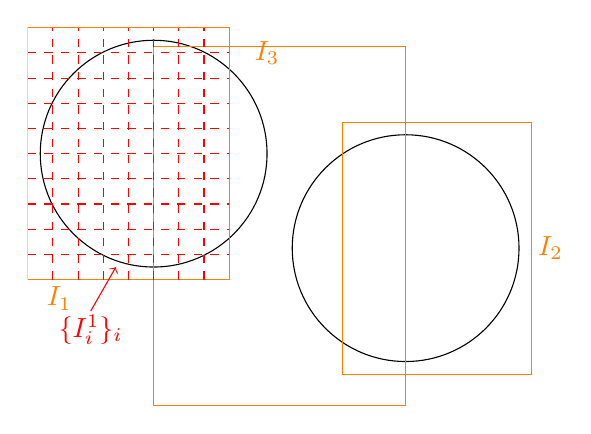
\begin{tikzpicture}[scale=0.8]
                \clip (-2,-4) rectangle (6.5,2);
                \draw (0,0) circle (1.8);
                \draw (4,-1.5) circle (1.8);
                \draw[orange] (-2,-2) rectangle (1.2,2);
                \draw[orange] (0,-4) rectangle (4,1.7);
                \draw[orange] (3,-3.5) rectangle (6,0.5);
                \draw[dashed, red] (-1.6,-2)--(-1.6,2);
                \draw[dashed, red] (-1.2,-2)--(-1.2,2);
                \draw[dashed, red] (-0.8,-2)--(-0.8,2);
                \draw[dashed, red] (-0.4,-2)--(-0.4,2);
                \draw[dashed, red] (0,-2)--(0,2);
                \draw[dashed, red] (0.4,-2)--(0.4,2);
                \draw[dashed, red] (0.8,-2)--(0.8,2);
                \draw[dashed,red] (-2,1.6)--(1.2,1.6);
                \draw[dashed,red] (-2,1.2)--(1.2,1.2);
                \draw[dashed,red] (-2,0.8)--(1.2,0.8);
                \draw[dashed,red] (-2,0.4)--(1.2,0.4);
                \draw[dashed,red] (-2,0)--(1.2,0);
                \draw[dashed,red] (-2,-1.6)--(1.2,-1.6);
                \draw[dashed,red] (-2,-1.2)--(1.2,-1.2);
                \draw[dashed,red] (-2,-0.8)--(1.2,-0.8);
                \draw[dashed,red] (-2,-0.4)--(1.2,-0.4);

                \node[orange] at (-1.5,-2.3) {$I_1$};
                \node[red] at (-1,-2.8) {$\{I_i^1\}_i$};
                \draw[red,->] (-1,-2.5)--(-0.6,-1.8);
                \node[orange] at (6.3,-1.5) {$I_2$};
                \node[orange] at (1.8,1.6) {$I_3$};
            \end{tikzpicture}
        \end{imgbox}
        Siano quindi $H_A =\{h\in H\, |\, J_h\cap A\neq \varnothing\}$ e $H_B =\{h\in H\, |\, J_h\cap B\neq \varnothing\}$. Allora $H_A\cap H_B=\varnothing$, altrimenti esisterebbe un $J_{\bar h}$ tale che $J_{\bar h}\cap A\neq \varnothing$ e $J_{\bar h}\cap B\neq \varnothing$. Ciò implicherebbe che $\operatorname{diam} J_{\bar h}\geq d$, il che è un assurdo per costruzione di $\{J_h\}_h$. Inoltre, per costruzione di $H_A$ e $H_B$, $H_A\cup H_B\subset H$, e quindi $\{J_h\}_{h\in H_A}\in \mc{R}(A)$ e $\{J_h\}_{h\in H_B}\in \mc{R}(B)$. Di conseguenza
        \[\begin{aligned}\mc{L}^n(A)+\mc{L}^n(B) &\leq \sum_{h\in H_A}v(J_h)+\sum_{h\in H_B}v(J_h)=\sum_{h\in H_A\sqcup H_B}\!\!v(J_h) = \substack{\text{ritornando alla}\\\text{notazione precedente}}\\ &= \sum_{j}\sum_{i=1}^{N_j}v(I_i^j)\underset{\eqref{eq: 1.6: 3}}{\leq} \sum_j\left( v(I_j)+\frac{\epsilon}{2^j} \right) = \sum_j v(I_j)+\sum_j\frac{\epsilon}{2^j} \\ & \leq \sum_j v(I_j)+\epsilon \underset{\eqref{eq: 1.6: 2}}< \mc{L}^n(A\cup B) +2\epsilon \end{aligned}\]
        quindi otteniamo 
        \[\mc{L}^n(A)+\mc{L}^n(B) < \mc{L}^n(A\cup B) +2\epsilon \]
        per cui, siccome non vi è dipendenza da $\epsilon$, per $\epsilon\to 0$ si ha la tesi.
        \item \textbf{\underline{Di Radón:}} Poiché $\mc{L}^n$ è metrica, dal Teorema di Carathéodory segue che $\mc{L}^n$ è boreliana (i.e. $\mc{B}(\R^n)\in M_{\mc{L}^n}$)
        \begin{itemize}
            \item \textbf{Borel-regolare:} Sia $A\subset \R^n$ qualsiasi. \hspace{\fill}\boxed{\textsc{tesi: }\exists\, B\in \mc{B}(\R^n)\ :\ B\supset A \;\land\; \mc{L}^n(B)=\mc{L}^n(A)}\\
            Se $\mc{L}^n(A)=+\infty$, la tesi è banale con $X=\R^n$, infatti $B\supset A$, quindi per monotonia $\mc{L}^n(B)\geq \mc{L}^n(A)=+\infty\Rarr \mc{L}^n(B)=+\infty$. Supponiamo quindi $\mc{L}^n(A)<+\infty$.\\
            Di conseguenza $\forall j \exists \{I_i^j\}_i\in \mc{R}(A)$ tale che 
            \[\sum_iv(I_i^j)<\mc{L}^n(A)+\frac{1}{j}<+\infty.\]
            Sia quindi $G_j:=\bigcup_iI_j^i\in \mc{G}$ (NB$^1$: $G_j\supset A$). Ossreviamo che per definizione di $\mc{L}^n$ 
            \begin{equation}\label{eq: 1.6: 4}
                \mc{L}^n(G_j)\leq \sum_iv(I_i^j)\leq \mc{L}^n(A)+\frac{1}{j}
            \end{equation}
            Poniamo infine $B=\bigcap_jG_j\in \mc{B}(R^n)$ (NB$^2$: $B\supset A$, segue da NB$^1$). Scelto allora un qualsiasi $j$,
            \[\mc{L}^n(B)\leq \mc{L}^n(G_j)\underset{\eqref{eq: 1.6: 4}}{\leq} \mc{L}^n(A)+\frac{1}{j}\]
            quindi, per $j\to+\infty$, $\mc{L}^n(B)\leq \mc{L}^n(A)$. Per monotonia di $\mc{L}^n$ e NB$^2$, $\mc{L}^n(A)\leq \mc{L}^n(B)$, da cui la tesi.
            \item \textbf{Di Radón:} 
            Sia $K\in \mc{K}$, allora per il Teorema di Heine-Borel, $K$ è limitato. \hspace{\fill}\boxed{\textsc{tesi: }\mc{L}^n(K)<+\infty}\\
            Allora Esiste un intervallo aperto (N.B. i lati hanno lunghezza finita) $I\subset \R^n$ tale che $K\subset I$, allora $\{I\}\in \mc{R}(K)$. Di conseguenza $\mc{L}^n(K)\leq v(I)=\inf_{\mc{R}(K)}S=S(\{I\})=v(I)<+\infty$.
            \qedhere
        \end{itemize}
    \end{enumerate}
\end{proof}

\begin{definition}
  La misura esterna $\mc{L}^{n}$ definita in Teorema \ref{thm: lebesgue grande} è detta "misura esterna di Lebesgue n-dimensionale".
\end{definition}
Il seguente risultato elenca alcune proprietà della misura esterna di Lebesgue.

\begin{shadedTheorem}[$**$| Lebesgue - piccolo]\label{thm: lebesgue piccolo}
  Valgono i seguenti fatti:
  \begin{enumerate}
      \item Per ogni $a\in \R^n$, si ha $\mc{L}^n(\{a\})=0$;
      \item Se $I$ è un intervallo aperto in $\R^n$, si ha $\mc{L}^n(I)=v(I)$; 
      \item Per ogni $E\in \P(\R^n)\setminus\{\varnothing\}$ e per ogni $\tau\in \R^n$ si ha:
      \begin{enumerate}
          \item $\mc{L}^n(E+\tau)=\mc{L^n}(E)$;
          \item Se $E\in M_{\mc{L}^n}$, allora $E+\tau\in M_{\mc{L}^n}$;
      \end{enumerate}
      \item Per ogni $E\in \P(\R^n)\setminus\{\varnothing\}$ e per ogni $\rho\in\;]0,+\infty[$ si ha:
      \begin{enumerate}
          \item $\mc{L}^n(\rho E)=\rho^n\mc{L}^n(E)$;
          \item Se $E\in M_{\mc{L}^n}$, allora $\rho E\in M_{\mc{L}^n}$;
      \end{enumerate}
  \end{enumerate}
\end{shadedTheorem}
\begin{proof}~
  \begin{enumerate}[label=$(\arabic*)$] 
      \item Sia $a\in \R^n$, sia $\epsilon>0$ arbitrario. \hspace{\fill}\boxed{\textsc{tesi: }\mc{L}^n(\{a\})=0}\\ 
      Sia ora $I_\epsilon = ]-\epsilon, \epsilon[^n+a$ un intervallo aperto contenente $a$. Allora $I_\epsilon\in \mc{R}(\{a\})$, quindi $\mc{L}^n(\{a\}) = \inf_{\mc{R}(\{a\})}S\leq S(\{I_\epsilon\})=v(I_\epsilon)=(2\epsilon)^n$. Poiché $\mc{L}^n(\{a\})$ non dipende da $\epsilon$, per $\epsilon\to 0$ si ha la tesi.
      \item Sia $I$ un intervallo aperto di $\R^n$ qualsiasi.Osserviamo che $\{I\}\in \mc{R}(I)$. \hspace{\fill}\boxed{\textsc{tesi: }\mc{L}^n(I)=v(I)}\\
      Allora $\mc{L}^n(I)=\inf_{\mc{R}(I)}S\leq S(\{I\})=v(I)$, quindi è sufficiente provare la \tesi[ 2]{\mc{L}^n(I)\geq v(I)}

      Siano $\{I_j\}_\in \mc{R}(I)$, $I=]a_1,b_1[\;\times\dots\times\;]a_n,b_n[$. Sia $\varepsilon>0$ sufficientemente piccolo affinché 
      \[J_\varepsilon := [a_1+\varepsilon,b_1-\varepsilon]\;\times\dots\times\;[a_n+\varepsilon,b_n-\varepsilon]\]
      abbia senso (ovvero $\forall i, a_i+\epsilon <b_i-\epsilon$). Allora $J_\epsilon$ è un compatto e $J_\epsilon\subset I\subset \bigcup_jI_j$. Allora per definizione di compattezza, $J_\epsilon$ ammette un sottoricoprimento finito, ovvero $\exists\;\{j_1, \dots, j_n\}\;:\; J_\epsilon^\circ\subset J\epsilon\subset \bigcup_{i=1}^nI_{j_i}$, quindi 
      \[\mc{L}^n(I) = \inf_{\mc{R}(I)}S\geq v(J_\epsilon^\circ)=(b_1-a_1-2\epsilon)\cdot \ldots\cdot (b_n-a_n-2\epsilon)\]
      quindi per $\epsilon \to 0$, $v(J_\epsilon^\circ)\to v(I)$, per cui $\mc{L}^n(I)\geq v(I)$, da cui segue la tesi.

      \item 
      \begin{enumerate}
          \item Sia $E\in\mc{P}(\R^n)\setminus\{\varnothing\}, \tau \in \R^n$. Sia $\{I_j\}_j\in\mc{R}(E)$. \hspace{\fill}\boxed{\textsc{tesi: }\mc{L}^n(E+\tau)=\mc L^n(E)}\\ 
          Allora banalmente $\{I_j+\tau\}_j\in\mc{R}(E+\tau)$.  Inoltre si ha $\forall I,\ v(I)=v(I+\tau)$, quindi 
          \[\mc{L}^n(E+\tau)=\inf_{\mc{R}(E+\tau)}S\leq S(\{I_j+\tau\}_j) = \sum_jv(I_j+\tau)=\sum_jv(I_j)=S(\{I_j\})\]
          quindi, passando all'estremo inferiore, $\mc{L}^n(E+\tau)\leq \mc{L}^n(E)$. Da questo segue che 
          \[\mc{L}^n(E)=\mc{L}^n(E+\tau+(-\tau))\leq \mc{L}^n(E+\tau)\leq \mc{L}^n(E)\ \implies \ \mc{L}^n(E)=\mc{L}^n(E+\tau)\]
          \item Siano $E\in \mc{M}_{\mc{L}^n}$ e $\tau \in \R^n$, $A\in \mc{P}(\R^n)$.  \tesi{E+\tau\in M_{\mc{L}^n}}
          \renewcommand{\arraystretch}{1.8}
          \[\begin{array}{c}
              \mc{L}^n(A\cap(E+\tau))+\mc{L}^n(A\cap \underbrace{(E+\tau)^c}_{E^c+\tau}) = \mc{L}^n(((A-\tau)+\tau)\cap (E+\tau))+ \mc{L}^n(((A-\tau)+\tau)\cap (E^c+\tau))=\\
              =\mc{L}^n(((A-\tau)\cap E)+\tau)+ \mc{L}^n(((A-\tau)\cap E^c)+\tau)=\mc{L}^n((A-\tau)\cap E)+ \mc{L}^n((A-\tau)\cap E^c)=\\
              =\mc{L}^n(A-\tau) = \mc{L}^n(A).
          \end{array}\]
          \renewcommand{\arraystretch}{1}
      \end{enumerate}
      \item 
      \begin{enumerate}
          \item Siano $E\in \mc{P}(R^n)\setminus \{\varnothing\}$, $\rho\in\;]0,+\infty[$. \tesi{\mc{L}^n(\rho E)=\rho^n\mc{L}^n(E)} \\
          Osserviamo che $\forall I$ intervallo, $v(\rho I)=\rho^nv(I)$. Sia $\{I_j\}_j\in \mc{R}(E)$ qualsiasi. Allora $\{\rho I_j\}_j\in \mc{R}(\rho E)$. Di conseguenza 
          \[\mc{L}^n(\rho E)=\inf_{\mc{R}(\rho E)}S\leq S(\{\rho I_j\}_j)=\sum_jv(\rho I_j)=\sum_j\rho^nv(I_j)=\rho^n\sum_jv(I_j)=\rho ^nS(\{I_j\}_j)\]
          quindi passando all'estremo inferiore segue che $\mc{L}^n(\rho E)\leq \rho^n\mc{L}^n(E)$. Da questo segue che
          \[\mc{L}^n(E)=\mc{L}^n(\rho^{-1}\rho E)\leq \rho^{-n}\mc{L}^n(\rho E)\leq \mc{L}^n(E)\ \implies \ \mc{L}^n(\rho E)=\rho^n\mc{L}^n(E)\]
          \item Sia $E\in M_(\mc{L}^n), \rho \in\;]0,+\infty[$. Fissato $A\in \mc{P}(\R^n)$, \tesi{\rho E\in M_{\mc{L}^n}}
          \renewcommand{\arraystretch}{1.8}
          \[\begin{array}{c}
              \mc{L}^n(A\cap \rho E)+\mc{L}^n(A\cap \underbrace{(\rho E)^c}_{\rho E^c}) = \mc{L}^n(\rho\rho^{-1}A \cap \rho E)+\mc{L}^n(\rho \rho^{-1}A \cap \rho E^c)=\\
              = \mc{L}^n (\rho(\rho^{-1}A \cap E))+\mc{L}^n(\rho(\rho^{-1}A\cap E^c)) = \rho^n[\mc{L}^n(\rho^{-1}A\cap E)+\mc{L}^n(\rho^{-1}A\cap E^c)]=\\=\rho^n\mc{L}^n(\rho^{-1}A)=\cancel{\rho^n\rho^{-n}}\mc{L}^n(A).
          \end{array}\]\qedhere
          \renewcommand{\arraystretch}{1}
      \end{enumerate}
  \end{enumerate}
\end{proof}

\begin{exc} Provare le seguenti identità:
  \[
  \begin{gathered}
  (E+\tau)^{c}=E^{c}+\tau, \quad(A+\tau) \cap(B+\tau)=(A \cap B)+\tau \\
  (\rho E)^{c}=\rho E^{c}, \quad(\rho A) \cap(\rho B)=\rho(A \cap B) .
  \end{gathered}
  \]
\end{exc}

\begin{example}Si ha $\mc{L}^{n}\left(\mathbb{Q}^{n}\right)=0$. L'insieme $\mathbb{Q}^{n}$ è misurabile.
\end{example}

\begin{remark} Utilizzando l'insieme di Cantor si può provare che esistono sottoinsiemi di $\mathbb{R}$ che sono misurabili rispetto a $\mc{L}^{1}$ ma non sono Boreliani: sia $\{C_j\}_{j \in \N} \subset \mc{P}(\R^n)$ la successione di insiemi definita ricorsivamente ponendo $C_0 := [0, 1]^n$ e $C_{j+1}$ è l'insieme ottenuto da $C_j$ rimuovendo tutti i terzi medi (aperti) di lunghezza $\sfrac{1}{3^j}$. L'insieme di Cantor è definito quindi come $C := \bigcap_{j \in \N} C_j$. \\
  \begin{tikzpicture}[decoration=Cantor set,very thick]
    
    \draw  (0,0.5) -- (3,0.5);
    \draw decorate{ (0,0) -- (3,0) };
    \draw decorate{ decorate{ (0,-.5) -- (3,-.5) }};
    \draw decorate{ decorate{ decorate{ (0,-1) -- (3,-1) }}};
    \draw decorate{ decorate{ decorate{ decorate{ (0,-1.5) -- (3,-1.5) }}}};
    \node at (-7,-0.5){
      \begin{minipage}{13cm}
        Possiamo osservare innanzitutto che l'insieme di Cantor è ottenuto come intersezione (numerabile) di chiusi, per cui è a sua volta un chiuso. Essendo limitato è inoltre un compatto. Inoltre la successione dei $\{C_j\}$ è decrescente e costituita da misurabili, quindi possiamo applicare il teorema di continuità dall'alto ottenendo che 
        \[\lim_{j\to +\infty} \mc L^1 (C_j) = \mc L^1(C).\]
      \end{minipage}
    };
  \end{tikzpicture}\\
  In particolare, ogni $C^j$ è dato dall'unione disgiunta di $2^j$ segmenti di lunghezza $\sfrac{1}{3^j}$, per cui 
  \[\mc L^1(C) = \lim_{j\to +\infty} \mc L^1 (C_j) = \lim_{j\to +\infty} \left( \frac{2}{3} \right)^j = 0\]
  In particolare, per monotonia $\P(C)\subset \mc M_{\mc L^1}$. 

  Verifichiamo ora che $\operatorname{card}( C )= \operatorname{card}(\R)$: al fine di questa dimostrazione, identifichiamo i numeri reali con il loro allineamento decimale in base 3. Allora l'operazione di rimozione che abbiamo effettuato consiste, al primo passo, a rimuovere tutto ciò che ha 1 come prima cifra decimale, al secondo tutto ciò che ha 1 come seconda cifra decimale e così via. Dobbiamo solo prestare attenzione ai decimali limitati, in quanto quelli che terminano con $1$ sono l'estremo inferiore dei segmenti che stiamo eliminando, e devono rimanere nell'insieme finale: per evitare questo problema è tuttavia sufficiente interpretare $0,1 = 0,0\bar{2}$ e così via. Iterando questo procedimento rimaniamo alla fine con numeri che hanno allineamenti decimali contenenti le sole cifre $0$ e $2$: sostituendo i simboli mediante la legge $0\mapsto 0$ e $2\mapsto 1$ possiamo interpretare questi numeri come allineamenti decimali in base 2 e osservare che in questo modo stiamo riscrivendo in un'altra base lo stesso intervallo $[0,1]$.

  Come diretta conseguenza di questa trattazione abbiamo quindi che 
  \[
  \operatorname{card}(\mathbb{R})=\operatorname{card}(C)<\operatorname{card}\left(\P({C})\right) \leq \operatorname{card}\left(\mc{M}_{\mc{L}^{1}}\right)
  \]
  A questo punto la conclusione segue subito dal fatto che $\operatorname{card}(\mc{B}(\mathbb{R}))=\operatorname{card}(\mathbb{R})$, per la dimostrazione del quale rimandiamo a $[\mathbf{1 5}]$.
\end{remark}
\begin{example}[Esistenza di insiemi non misurabili: l'esempio di Vitali] Consideriamo la seguente relazione di equivalenza in $[0,1]: x \sim y$ se $x-y \in \mathbb{Q}$. Grazie all'assioma della scelta possiamo poi "costruire" un insieme $E\subset [0,1]$ di rappresentanti delle classi di equivalenza. Se $\mathbb{Q} \cap\ [-1,1]=\left\{q_{i}\right\}_{i \in \mathbb{N}}$, poniamo infine $E_j = E + q_j$: allora $\mc L^1(E_j) = \mc L^1(E)$ e $\forall j, E_j\subset [-1,2]$. 
\begin{itemize}
  \item Verifichiamo inizialmente che $[0,1]\subset \bigcup_jE_j$: fissato $x\in [0,1]$, deve esistere un $e\in E$ tale che $x-e\in \Q$ (in particolare, poiché $x,e\in [0,1]$, $x-e\in [-1,1]$). Di conseguenza deve esistere un $j$ tale che $x-e = q_j$, per cui $x = e+q_j\in E+q_j = E_j$.
  \item Osserviamo quindi che gli $\{E_j\}_j$ sono a-2-a-2 disgiunti: siano infatti $i\neq j$, supponiamo per assurdo che esista $x\in E_i\cap E_j$. Si avrebbe quindi $x = e_1+q_i = e_2+q_j$ con $e_1,e_2\in E$, da cui $e_1-e_2 = q_j-q_i\in \Q$. Questo implicherebbe $e_1\sim e_2$, ovvero $e_1 = e_2$ per costruzione di $E$, da cui $q_i = q_j$ e $i = j$, assurdo.
\end{itemize}
Proviamo infine che $E$ non è misurabile: supponiamo per assurdo che lo sia, allora per il Piccolo Teorema di Lebesgue tutti gli $E_j$ avrebbero la sua stessa misura, da cui 
\[\textstyle 1 = \mc L^1([0,1]) \leq \mc L^1( \bigcup_jE_j)\leq \mc L^1([-1,2]) = 3.\tag{$*$}\]
In particolare, per $\sigma$-additività, avremmo 
\[\textstyle \mc L^1( \bigcup_jE_j) = \sum_j\mc L^1(E_j) = \sum_j\mc L^1(E).\]
A questo punto si configurano due casi: se $L^1(E) = 0$, la serie ha somma nulla (quando per ($*$) dovrebbe essere maggiore di $1$); se $L^1(E)>0$ la serie diverge in quanto la successione degli addendi e positiva e non infinitesma (quando per $(*)$ dovrebbe essere limitata). In entrambe le situazioni si configura un assurdo, per cui $E$ non può essere misurabile.
\end{example}
\begin{exc}[\footnote{Già incluso nell'Esempio, NdR}]Provare che se $i \neq j$ allora $E_{i} \cap E_{j}=\varnothing$.
\end{exc}
\begin{remark}Senza l'assioma della scelta è impossibile provare l'esistenza di insiemi non misurabili (Solovay, 1970).\end{remark}

\subsection{Misura esterna di Hausdorff}
\begin{shadedTheorem}[$*$| Premisura di Hausdorff]\label{thm: 1.8 premisura Hausdorff}
  Dati $E\in\P(\R^n)$ e $\delta >0$, indichiamo con $\mc R_\delta (E)$ la famiglia dai ricoprimenti numerabili $\{C_j\}_j$ di $E$ tali che $0<\operatorname{diam}C_j\leq \delta$ $\forall j$. Per $s\in [0,+\infty[$, poniamo anche 
  \[\alpha(s):=\frac{\pi^{s/2}}{\Gamma\left(\frac{s}{2}+1\right)},\qquad \Gamma(t):=\int_0^{+\infty} e^{-x}x^{t-1}\operatorname{d}\!x.\]
  Allora la funzione $\mc{H}^s_\delta:\P(\R^n)\to [0,+\infty]$ definita da
  \[\mc{H}^s_\delta(E):=\begin{cases}
       \inf\left\{\sum_j\alpha(s)\left( \frac{\operatorname{diam}C_j}{2} \right)^s\,\Big|\,\{C_j\}_j\in\mc{R}_\delta (E)\right\} & \text{ se } E\neq \varnothing\\
       0 & \text{ se } E = \varnothing
   \end{cases}\]
   è una misura esterna
\end{shadedTheorem}

\begin{remark}Si può provare che $\alpha(n)=\mc{L}^{n}\left(B_{1}^{(n)}\right)$, dove $B_{1}^{(n)}$ è la palla unitaria di $\mathbb{R}^{n}$. Per una dimostrazione di questo fatto, si veda per esempio [16, Ch. 2, Exercise 14].
\end{remark}

\begin{proof}Verifichiamo gli assiomi di misura esterna:
  \begin{enumerate}[label=$\roman*)$]
      \item Il primo assioma di misura esterna ($\mc H_\delta^s(\varnothing) = 0$) è verificato per definizione.
      \item Siano $E \subset F \subset \R^n$, vogliamo dimostrare che $\mc H_\delta^s(E) \le \mc H_\delta^s(F)$.\\
          Se $E = \varnothing$ è banale, altrimenti $\mc R_\delta(E) \supset \mc R_\delta(F)$, dunque $\inf_{\mc R_\delta(E)} S \le \inf_{\mc R_\delta(F)} S$ e perciò $\mc H_\delta^s(E) \le \mc H_\delta^s(F)$.
      \item Sia $\{E_j\}_{j \in J} \subset \mc P(\R^n)$ numerabile, vogliamo dimostrare la $\sigma$-subaddittività.\\
          Se $\sum_{j \in J} \mc H_\delta^s(E_j) = + \infty$ la tesi è banale, come nel caso in cui $\bigcup_{j \in J} E_j = \varnothing$, supponiamo dunque che la somma sia finita e la famiglia non vuota con almeno un insieme non vuoto.\\
          Sia $J^* := \{ j \in J | E_j \neq \varnothing\}$ che per ipotesi è non vuoto, la nostra nuova tesi diventa $\mc H_\delta^s(\bigcup_{j \in J^*} E_j) \le \sum_{j \in J^*} \mc H_\delta^s(E_j)$, somma che abbiamo già assunto finita (e perciò la misura di ogni singolo insieme nella famiglia è finita).\\
          Di conseguenza, fissato $\varepsilon > 0$, abbiamo che $\forall j \in J^*, \exists \{C_i^j\}_{i \in I_j} \in \mc R_\delta(E_j)$ tale che \[S(\{C_i^j\}_{i \in I_j}) \le \mc H_\delta^s(E_j) + \frac{\varepsilon}{2^j}.\]\\
          Osserviamo quindi che $\{C_i^j\}_{i \in I_j,j \in J^*} \in \mc R_\delta(\bigcup_{j \in J^*} E_j)$ e perciò \[\mc H_\delta^s\bigg(\bigcup_{j \in J^*} E_j\bigg) \le S(\{C_i^j\}_{i \in I_j, j \in J^*}) = \sum_{j \in J^*} S(\{C_i^j\}_{i \in I_j}) \le \varepsilon + \sum_{j \in J^*} \mc H_\delta^s(E_j).\]\\
          Quini, per $\epsilon \to 0$, si ha la tesi.
  \end{enumerate}        
\end{proof}

\begin{exc}Verificare col calcolo diretto che: $\alpha(0)=1, \quad \alpha(1)=2, \quad \alpha(2)=\pi, \quad \alpha(3)=\frac{4 \pi}{3}$.\end{exc}

\begin{shadedTheorem}[$**$| Hausdorff]\label{thm: 1.9 Hausdorff}
  Sia $s\in [0,+\infty[$ e $E\in \P(\R^n)$. Allora la funzione $\delta \mapsto \mc{H}^s_\delta(E)$ è monotona decrescente, quindi esiste 
  \[\mc{H}^s(E)=\lim_{\delta \to 0}\mc{H}^s_\delta(E).\]
  La mappa $\mc{H}^s:\P(\R^n)\to [0,+\infty]$ è una misura esterna metrica e Borel regolare. Essa è detta \say{misura di Hausdorff $s$-dimensionale $($in $\R^n)$}.
\end{shadedTheorem}
\begin{proof}~
  \begin{enumerate}[label=\textbf{\Large\arabic*.}, ref=\textbf{\underline{(\arabic*)}}]
      \item \textbf{\underline{Monotonia}:} Siano $\delta_1, \delta_2 \in \R \ :\  0<\delta_1 < \delta_2$. Vogliamo dimostrare che $\mc H_{\delta_1}^s(E) \le \mc H_{\delta_2}^s(E)$.\\
      Osserviamo che $\mc R_{\delta_1}(E) \supset \mc R_{\delta_2}(E)$, dunque $\inf_{\mc R_{\delta_1}(E)}S \le \inf_{\mc R_{\delta_2}(E)}S$, ovvero la tesi. Di conseguenza, per il teorema di esistenza di limite per funzioni monotone, esiste $\mc{H}^s_\delta(E)$.
      \item \textbf{\underline{Misura esterna}:} \begin{enumerate}[label=$\roman*)$]
          \item $\mc{H}^s(\varnothing)=\lim\limits_{\delta \to 0}\mc{H}^s_\delta(\varnothing)=\lim\limits_{\delta \to 0}0=0$;
          \item Siano $E,F\in \mc{P}(\R^n),\ E\subset S$. Allora $\forall \delta, \mc{H}^s_\delta(E)\leq \mc{H}^s_\delta(F)$, per cui facendo tendere $\delta$ a $0$, si ha $\mc{H}^s(E)\leq \mc{H}^s(F)$;
      \end{enumerate}
      N.B. Poiché $\mc{H}^s(E)=\lim\limits_{\delta \to 0}\mc{H}^s_\delta(E)$ e la funzione $\delta \mapsto \mc{H}^s_\delta(E)$ è decrescente, segue che $\forall \delta\ \mc{H}^s_\delta(E)\leq \mc{H}^s(E)$.
      \begin{enumerate}[resume,label=$\roman*)$]
          \item Sia $\{E_j\}_{j}$ numerabile. \tesi{\mc{H}^s\Bigl(\bigcup\nolimits_jE_j\Bigr)\leq \sum\nolimits_j\mc{H}^s(E_j)}\\
          Poiché $\mc{H}^s_\delta$ è una misura esterna si ha \[\mc{H}^s_\delta\Bigl(\bigcup\nolimits_jE_j\Bigr)\leq \sum\nolimits_j\mc{H}^s_\delta(E_j)\leq \sum\nolimits_j\mc{H}^s(E_j)\quad \forall \delta >0\]
          \[\underset{\delta \to 0}\implies \mc{H}^s\Bigl(\bigcup\nolimits_jE_j\Bigr) = \lim_{\delta \to 0}\mc{H}^s_\delta\Bigl(\bigcup\nolimits_jE_j\Bigr)\leq \sum\nolimits_j\mc{H}^s(E_j)\]
      \end{enumerate}
      \item \textbf{\underline{Metrica}:} Siano $A,B\in \mc{P}(\R)$ tali che $\operatorname{dist}(A,B)=d>0$. Poiché vale la $\sigma$-subadditività, è sufficiente provare la \tesi{\mc{H}^s(A\cup B)\geq\mc{H}^s(A)+\mc{H}^s(B)}\\
      Se $\mc{H}^s(A\cup B)=+\infty$, la tesi è banale. Supponiamo quindi $\mc{H}^s(A\cup B)<+\infty$. Allora per quanto detto precedentemente, anche $\mc{H}^s_\delta(A\cup B)<+\infty$. Proviamo innanzitutto che $\forall \delta <d$ si ha \[\mc{H}^s_\delta(A\cup B)\geq \mc{H}^s_\delta(A)+\mc{H}^s_\delta(B)\]
      Siano $\delta < d$ e $\epsilon >0$. Poiché
      $+\infty>\mc{H}^s_\delta(A\cup B)=\inf_{\mc{R}_\delta(A\cup B)}S$, esiste una famiglia $ \{C_j\}_j\in\mc{R}_\delta(A\cup B)$ tali che $S(\{C_j\}_j)<\mc{H}^s_\delta(A\cup B)+\epsilon\ \ (*)$. Per costruzione si ha quindi che $\forall j,$ $C_j$ non interseca sia $A$ che $B$. Definiamo $J_A:=\{j\in J\,|\,C_j\cap A\neq \varnothing\}$ e osserviamo che $J_A\neq \varnothing$ e $\{C_j\}_{j\in \A}\in \mc{R}_\delta (A)$; analogamente per $J_B$. Osserviamo inoltre che $J_A\sqcup J_B\subset J$, quindi 
      \[\begin{aligned}\mc{H}^s_\delta(A)+\mc{H}^s_\delta(B)&\leq S(\{C_j\}_{j\in J_A})+S(\{C_j\}_{j\in J_B})= \sum_{j\in J_A}\alpha(s)\left( \frac{\operatorname{diam}C_j}{2} \right)^s+\sum_{j\in J_B}\alpha(s)\left( \frac{\operatorname{diam}C_j}{2} \right)^s=\\&=\sum_{j\in J_A\sqcup J_B}\alpha(s)\left( \frac{\operatorname{diam}C_j}{2} \right)^s\leq \sum_{j\in J}\alpha(s)\left( \frac{\operatorname{diam}C_j}{2} \right)^s=S(\{C_j\}_{j\in J})\underset{(*)}<\mc{H}^s_\delta(A\cup B)+\epsilon\end{aligned}\] 
      per cui, per $\epsilon \to 0$, si ha che $\mc{H}^s_\delta(A\cup B)\geq \mc{H}^s_\delta(A)+\mc{H}^s_\delta(B)$. Passando al limite per $\delta \to 0$, segue la tesi. 
      \item \textbf{\underline{Borel-Regolare}:} Poiché $\mc{H}^s$ è metrica, per il teorema di Carathéodory segue che $\mc{H}^s$ è boreliana. Rimane da provare la Borel-regolarità: sia $A\in \mc{P}(X)$. \tesi{\exists B\in \mc{B}(X)\ :\ B\supset A\ \land\ \mc{H}^s(A)=\mc{H}^s(B)}\\
      Se $\mc{H}^s(A)=+\infty$, basta prendere $B=\R^n$. Allora $B=\R^n\supset A$ e $\mc{H}^s(\R^n)=+\infty$ per monotonia. Supponiamo quindi $\mc{H}^s_\delta(A)<+\infty$. Allora per ogni $j\in \Z^+, \mc{H}^s_\frac{1}{j}(A)\leq \mc{H}^s(A)<+\infty$. Conseguentemente, esiste una famiglia $\{C_i^j\}_{i\in I_j}\in \mc{R}_{\frac{1}{j}}(A)$ tale che
      \[S(\{C^j_i\}_{i\in I_j})<\mc{H}^s_\frac{1}{j}(A)+\frac{1}{j} \tag{$**$}\]
      dove $S(\{C^j_i\}_{i\in I_j}) = \sum_{i\in I_j}\alpha(s)\left(\frac{\operatorname{diam}C^j_i}{2}\right)^s=\sum_{i\in I_j}\alpha(s)\left(\frac{\operatorname{diam}\bar C^j_i}{2}\right)^s$  in quanto $\operatorname{diam}C = \operatorname{diam}\bar C$. Consideriamo ora $B_j=\bigcup_{i\in I_j}\bar C^j_i\in \mc{B}(\R^n)$ in quanto tutti i $C^j_i$ sono chiusi. Poiché $\{C_i^j\}_{i}\in \mc{R}_\frac{1}{j}(A)$, allora $A\subset \bigcup_i C_i^j\subset \bigcup \bar C_j^i \subset B_j$. 

      Abbiamo quindi $B\supset A$. Rimane quindi da provare l'uguaglianza delle misure di Hausdorff. Per monotonia vale già un verso della disuguaglianza, rimane pertanto da provare la \tesi[ 2]{\mc{H}^s(B)\leq \mc{H}^s(A)}\\
      Abbiamo quindi che 
      \[\mc{H}^s_{\frac{1}{j}}(B)\underset{(\bullet)}\leq\sum_j\alpha(s)\left( \frac{\operatorname{diam}\bar C_i^j}{2}\right)^s\underset{(**)}\leq \mc{H}^s_\frac{1}{j}(S)+\frac{1}{j}\]
      (\textbullet) in quanto $\{\bar C_i^j\}\in \mc{R}_\frac{1}{j}(B_j)$. Di conseguenza, per $j\to +\infty$, segue la tesi.\qedhere
  \end{enumerate}
\end{proof}

\begin{exc}Provare che se $X$ è uno spazio metrico, allora per ogni sottoinsieme $C$ di $X$ si ha $\operatorname{diam} C=\operatorname{diam} \bar{C}$. 
\end{exc}

Alcune ulteriori proprietà della misura esterna di Hausdorff sono raccolte in questo teorema di cui non proviamo il punto (2) e lasciamo per esercizio le parti dei punti (3) e (4) che replicano quasi identicamente gli argomenti usati per provare le corrispondenti asserzioni in Teorema \ref{thm: lebesgue piccolo}. La dimostrazione del punto (2) è un argomento (basato sulla disuguaglianza isodiametrica) che non abbiamo tempo di affrontare. Gli interessati possono consultare, per esempio, $[\mathbf{3}, \mathbf{11}]$.


\begin{shadedTheorem}[$*$| Hausdorff - piccolo]\label{thm: hausdorff piccolo}
  Si ha:
  \begin{enumerate}
    \item $\mc{H}^{0}=\#$ (misura del conteggio);
    \item $\mc{H}^{n}=\mc{L}^{n}\left(\right.$in $\left.\mathbb{R}^{n}\right)$ - non lo dimostriamo;
    \item Per ogni insieme non vuoto $E \subset \mathbb{R}^{n}$ e per ogni $\tau \in \mathbb{R}^{n}$ si ha:
    \begin{itemize}
      \item $\mc{H}^{s}(E+\tau)=\mc{H}^{s}(E)$
      \item Se $E \in \mc{M}_{\mc{H}^{s}}$ allora $E+\tau \in \mc{M}_{\mc{H}^{s}}$;
    \end{itemize}
    \item Per ogni insieme non vuoto $E \subset \mathbb{R}^{n}$ e per ogni $\rho \in \mathbb{R}^{+}$si ha:
    \begin{itemize}
      \item $\mc{H}^{s}(\rho E)=\rho^{s} \mc{H}^{s}(E)$;
      \item Se $E \in \mc{M}_{\mc{H}^{s}}$ allora $\rho E \in \mc{M}_{\mc{H}^{s}}$;
    \end{itemize}
  \end{enumerate}
\end{shadedTheorem}
\begin{proof}~
  \begin{enumerate}
      \item \begin{itemize}
          \item Se $E = \varnothing$, la tesi segue banalmente.
          \item Se $E = \{p\} \in \R^n$, si ha che $\forall \delta > 0$ vale \[\mc H_\delta^0(E) = \inf\left\{\left.\sum_j \alpha(0)\left(\frac{\operatorname{diam}(C_j)}{2}\right)^0\right|\{C_j\}_j \in \mc R_\delta(E)\right\} = \inf\{\#\{C_j\}_j |\{C_j\}_j \in \mc R_\delta(E)\}\] Dato che $E \neq \varnothing$ abbiamo $\forall \{C_j\}_j \in \mc R_\delta(E),\#\{C_j\}_j \geq 1$, quindi $\mc H_\delta^0(E) \geq 1$.\\ Inoltre, $\operatorname{diam}(B_{\delta/3}(p)) = \frac{2\delta}{3}<\delta \Rarr B_{\delta/3}(p) \in \mc R_\delta(E)$, dunque $1 \leq \mc H_\delta^0(E) \leq S(B_{\delta/3}(p)) \leq 1 \Rarr \forall \delta > 0 , \mc H_\delta^0(E) = 1 \Rarr \mc H^0(E) = 1$.
          \item Sia $E$ finito. Allora $E = \bigcup_j \{p_j\}$ con $\forall i \neq j, d(p_i,p_j) > 0$ e dal teorema di \textbf{\textit{Carathéodory}} segue $\mc H^0 (E) = \sum_j \mc H(p_j) = \sum_j 1 = \#E$.
          \item Sia $E$ un insieme infinito. Allora $\forall N > 0, \exists F \subset E | \#F = N \Rarr \mc H^0(E) > \mc H^0(F)=\#F=N \Rarr \mc H^0(E) = +\infty$.
      \end{itemize}
      \item La dimostrazione del secondo punto viene omessa.
      \item Sia $E \in \mc P(\R^n)$ e $\tau \in \R^n$. \\ Posto $\delta > 0$ si ha $\{C_j\}_j \in \mc R_\delta(E) \Rarr \{C_j+\tau\}_j \in \mc R_\delta(E+\tau)$ dunque \[\mc H_\delta^s(E+\tau) = \inf_{\mc R_\delta(E+\tau)}S \leq S(\{C_j+\tau\}_j) = S(\{C_j\}_j) \Rarr \mc H_\delta^s(E+\tau) \leq \mc H_\delta^s(E)\]. Ora, $\mc H_\delta^s(E) = \mc H_\delta^s((E+\tau)-\tau) \leq \mc H_\delta^s(E+\tau)$, dunque $\forall \delta > 0, \mc H_\delta^s(E)=\mc H_\delta^s(E+\tau)\Rarr \mc H^s(E+\tau) = \mc H^s(E+\tau)$. \\ La dimostrazione del secondo punto di questo terzo punto è  analoga a quella per la misura di Lebesgue (Teorema \ref{thm: lebesgue piccolo}).
      \item Sia $\varnothing \neq E \in \mc P(\R^n)$ e siano $\rho ,\delta \in ]0,+\infty[$. Si ha che $\{C_j\}_j \in \mc R_\delta(E) \Rarr \{\rho C_j\}_j \in \mc R_{\rho \delta}(\rho E)$ e quindi \[\mc H_{\rho \delta}^s(\rho E) \leq S(\{\rho C_j\}_j) = \rho ^sS(\{C_j\}_j) \Rarr \mc H_{\rho \delta}^s(\rho E) \leq \rho ^s \mc H_{\delta}^s(E)\] Abbiamo anche \[\mc H_{\delta}^s(E) = \mc H_{\frac{1}{\rho }\rho \delta}^s(E) \leq \frac{1}{\rho ^s}\mc H_{\rho \delta}^s(\rho E)\] E quindi $\mc H_{\rho \delta}^s(\rho E) = \rho ^s\mc H_{\delta}^s(E)$. Mandando $\delta$ a $0$ segue la tesi. \\ La dimostrazione del secondo punto di questo quarto punto è  analoga a quella per la misura di Lebesgue (Teorema \ref{thm: lebesgue piccolo}).
  \end{enumerate}
\end{proof}

\begin{exc}Relativamente a Teorema \ref{thm: hausdorff piccolo}:

\begin{itemize}
  \item Provare che, per ogni $C \subset \mathbb{R}^{n}$ e per ogni $\rho \in \mathbb{R}^{+}$, si ha $\operatorname{diam}(\rho C)=\rho \operatorname{diam}(C)$;

  \item Provare il secondo punto di (3) ed il secondo punto di (4).
\end{itemize}
\end{exc}
\noindent Attraverso le proprietà della misura di Hausdorff si può definire una nozione di dimensione per i sottoinsiemi di $\mathbb{R}^{n}$.

\begin{proposition}[$*$]\label{prop: 1.4 dimensione Hausdorff} Se $\mc{H}^{s}(E)<+\infty$, con $E \subset \mathbb{R}^{n}$ e $s \geq 0$, allora $\mc{H}^{t}(E)=0$ per ogni $t>s$. Inoltre, per ogni $t>n$ si ha $\mc{H}^{t}\left(\mathbb{R}^{n}\right)=0$. Conseguentemente, per ogni $E \subset \mathbb{R}^{n}$, l'insieme
\[
R(E):=\left\{t \in[0,+\infty) \mid \mc{H}^{t}(E)=0\right\}
\]
è una semiretta destra che include $(n,+\infty)$. La "dimensione di Hausdorff" dell'insieme $E \subset \mathbb{R}^{n}$ è definita come il numero
\[
\operatorname{dim}_{H}(E):=\inf R(E) \leq n
\]
\end{proposition}
\begin{proof}
  \begin{itemize}
      \item Siano $E \in \mc P(\R^n), s \in [0,+\infty[$ tali che $\mc H^s(E) < +\infty$ e sia $t>s$. Per la dimostrazione precedente, con $\delta > 0$ si ha $\mc H_{\delta}^s(E) \leq \mc H^s(E) < +\infty$, dunque $\exists \{C_j\}_j \in \mc R_\delta(E):$ \[\sum_j \alpha(s) \left(\frac{\operatorname{diam}(C_j)}{2}\right)^s < \mc H_{\delta}^s(E) +1 \leq \mc H^s(E) + 1 < +\infty\]. Allora si ha 
      \[\begin{aligned}\mc H_{\delta}^t(E) &\leq \sum_j \alpha(t) \left(\frac{\operatorname{diam}(C_j)}{2}\right)^t = \frac{\alpha(t)}{\alpha(s)}\sum_j \alpha(s) \left(\frac{\operatorname{diam}(C_j)}{2}\right)^s \left(\frac{\operatorname{diam}(C_j)}{2}\right)^{t-s} \leq \\ &\leq\frac{\alpha(t)}{\alpha(s)} \left(\frac{\delta}{2}\right)^{t-s}\sum_j \alpha(s) \left(\frac{\operatorname{diam}(C_j)}{2}\right)^s \leq  \frac{\alpha(t)}{\alpha(s)} \left(\frac{\delta}{2}\right)^{t-s} (\mc H^s(E) + 1)\end{aligned}\] Dunque mandando $\delta$ a $0$ otteniamo $\mc H^t(E) \leq 0 \Rarr \mc H^t(E) = 0$.
      \item Sia $t>n$. Osserviamo che $\R^n = \bigcup_{j=0}^{+\infty} B_j(0)$ e ovviamente $\mc H^n (B_j(0)) = \mc L^n(B_j(0)) = \mc L^n(\bar{B}_j(0)) < +\infty$, dunque la $\forall j \in \N, \mc H^t(B_j(0)) = 0$ e per la $\sigma$-subadditività della misura di Hausdorff si ha $\mc H^t(\R^n) = 0$ 
      \item Sia $E \in \mc P(\R^n)$ e siano $s \in R(E)$ e $t>s$. Per quanto appena detto, $\mc H^t(E) = 0$, dunque $t \in R(E)$.
      \item Sia $t > n$, allora $t \in R(\R^n) \Rarr \forall E \in \mc P(\R^n), t \in R(E)$.
      \item Dai punti seguenti segue che $n = \inf]n,+\infty[ \geq \inf R(E) = \dim_{\mc H} E$
  \end{itemize}
\end{proof}

\begin{corollary}[$*$]\label{cor: 1.2 Hausdorff non Radon}
  La misura esterna di Haudorff $\mc{H}^{s}$ in $\mathbb{R}^{n}$ non è di Radón, eccetto che per $s \geq n$.
\end{corollary}
\begin{proof}~
  \begin{enumerate}[label=$(\roman*)$]
    \item $\mc{H}^s$ è di Radón in quanto coincide con $\mc{L}^n$.
    \item Se $t>n$, $\mc{H}^t$ è di Radón in quanto $\mc{H}^t(\R^n)=0$, quindi per monotonia $\mc{H}^t(E)=0\ \forall E\in \P(\R^n)$.
    \item Sia $s<n$, verifichiamo che $\mc{H}^s$ non è di Radón fornendo un controesempio: supponiamo per assurdo che $\mc{H}^s([0,1])<+\infty$, allora per la proposizione precedente $\mc{H}^n([0,1]^n)=0$, quindi $0=\mc{H}^n([0,1]^n)=\mc{L}^n([0,1]^n)=1$. Assurdo.\qedhere
  \end{enumerate}
\end{proof}

\begin{example}Sia $C$ l'insieme di Cantor. Non è facile verificare che esiste $s$ tale che $\mc{H}^{s}(C) \in]0,+\infty[$, ma se proviamo a supporre che esista allora troviamo facilmente che deve essere $s=\operatorname{dim}_{H}(C)=\sfrac{\ln 2}{\ln 3}$. Questo ci consente di "scommettere" che $C$ abbia effettivamente dimensione di Hausdorff pari a $\ln 2 / \ln 3$.\\
Osserviamo inizialmente che $C_2 = (\sfrac{1}{3}C_1)\cup (\sfrac{1}{3}C_1+\sfrac{2}{3})$ e che, in generale, $C_{k+1} = (\sfrac{1}{3}C_k)\cup (\sfrac{1}{3}C_k+\sfrac{2}{3})$. Questo ci porta a scrivere quindi la relazione $C = (\sfrac{1}{3}C)\cup (\sfrac{1}{3}C+\sfrac{2}{3})$, dove $\sfrac{1}{3}C$ e $\sfrac{1}{3}C+\sfrac{2}{3}$ sono insiemi a distanza positiva. In particolare, ricordando che $\mc H^s$ è metrica e supponendo (non è detto che ciò sia vero, lo proveremo successivamente) che esista un $s$ tale per cui $\mc H^s(C)\in\ ]0,+\infty[$,
\[\mc H^s(C) = \mc H^s\left(\frac{1}{3}C\right)+\mc H^s\left(\frac{1}{3}C+\frac{2}{3}\right) = 2 \left(\frac{1}{3}\right)^s \mc H^s(C).\]
Siccome abbiamo supposto $\mc H^s(C)\neq 0$, possiamo dividere, ottenendo 
\[1 = \frac{2}{3^s} \implies s = \frac{\ln 2}{\ln 3}.\]
Se tale $s$ esiste, quindi, vale $\sfrac{\ln 2}{\ln 3}$: rimane da provare che effettivamente le ipotesi che abbiamo fatto sono giustificate, ovvero che $\mc H^s(C) \in\ ]0,+\infty[$. Calcolando la misura di Hausdorff dell'insieme di Cantor, otteniamo infatti 
\[\mc H^{\frac{\ln 2}{\ln 3}} (C) = \alpha\left(\frac{\ln 2}{\ln 3}\right)\]
per cui la misura di Hausdorff di $C$ è effettivamente $\operatorname{dim}_{H}(C)=\sfrac{\ln 2}{\ln 3}$.\\
Per una dimostrazione più completa si faccia riferimento, per esempio, a [4, Theorem 1.14] oppure a [16, Ch. 7, Theorem 2.1].
\end{example}

\begin{definition}[Misura]Sia $X$ un insieme e $\mc{A}$ una $\sigma$-algebra in $X$. Allora, una "misura su $\mc{A}$ " è una funzione $\mu: \mc{A} \rightarrow[0,+\infty]$ tale che:
  \begin{enumerate}[label=$(\roman*)$]
    \item $\mu(\varnothing)=0$;
    \item se $\left\{E_{j}\right\}$ è una famiglia numerabile di insiemi in $\mc{A}$ a-due-a-due disgiunti, allora $\mu\left(\cup_{j} E_{j}\right)=\sum_{j} \mu\left(E_{j}\right)$.
  \end{enumerate}
  La terna $(X, \mc{A}, \mu)$ è detta "spazio con misura".
\end{definition}
Come conseguenza di Teorema \ref{thm: proprietà misurabili} e Proposizione \ref{prop: misurabili sigma-algebra}, otteniamo subito il seguente risultato.

\begin{proposition}[$\circ$] \label{prop: misura esterna è misura}Se $\varphi$ è una misura esterna sull'insieme $X$, allora $\left(X, \mc{M}_{\varphi},\left.\varphi\right|_{\mc{M}_{\varphi}}\right)$ è uno spazio con misura.
\end{proposition}
\begin{proof}~
  \begin{enumerate}[label=$(\roman*)$]
    \item $\phi(\varnothing)=0$ per assioma di misura esterna;
    \item se $\left\{E_{j}\right\}$ è una famiglia numerabile di insiemi in $\mc{M}_\phi$ a-due-a-due disgiunti, allora $\phi\left(\cup_{j} E_{j}\right)=\sum_{j} \mu\left(E_{j}\right)$ per il Teorema \ref{thm: proprietà misurabili}.
  \end{enumerate}
\end{proof}

\begin{example}La "misura di Lebesgue" $\left.\mc{L}^{n}\right|_{\mc{M}_{\mc{L}^{n}}}$ e la "misura di Hausdorff" $\left.\mc{H}^{s}\right|_{\mc{M}_{\mc{H}^{s}}}$. Per semplicità esse sono indicate con $\mc{L}^{n}$ and $\mc{H}^{s}$, rispettivamente.
\end{example}

\begin{remark}Ci si può chiedere se una misura provenga sempre da una misura esterna nel modo indicato in Proposizione \ref{prop: misura esterna è misura}. Una risposta quasi affermativa è data dal seguente risultato (vedasi [5, Theorem 4.47]): 
\end{remark}

\begin{shadedTheorem}
  Se $(X, \mc{A}, \mu)$ è uno spazio con misura, allora esiste una misura esterna $\varphi$ su $X$ tale che $\mc{A} \subset \mc{M}_{\varphi}$ e $\left.\varphi\right|_{\mc{A}}=\mu$.
\end{shadedTheorem}



\chapter{Funzioni misurabili e integrale}\label{ch: 2}
%\section{Funzioni misurabili.}
\begin{boxdef}[Funzione misurabile]
    Siano $(X, \mc{A}, \mu)$ e $(Y, \tau)$, rispettivamente, uno spazio con misura e uno spazio topologico. Allora una funzione $f: X \rightarrow Y$ si dice "misurabile" se per ogni $G \in \tau$ si ha $f^{-1}(G) \in \mc{A}$.
\end{boxdef}
\begin{oss}Consideriamo uno spazio misurabile $(X, \mc{A}, \mu)$ e supponiamo che $X$ sia anche uno spazio topologico con la topologia inclusa in $\mc{A}$. Inoltre, siano $Y$ uno spazio topologico e $f: X \rightarrow Y$ una funzione continua. Allora $f$ è misurabile. Esempi di situazioni di questo tipo sono:
\begin{itemize}
  \item $\left(\mathbb{R}^{n}, \mc{M}_{\mc{L}^{n}},\left.\mc{L}^{n}\right|_{\mc{M}_{\mc{L}^{n}}}\right), f: \mathbb{R}^{n} \rightarrow \overline{\mathbb{R}}$ continua;
  \item $\left(\mathbb{R}^{n}, \mc{M}_{\mc{H}^{s}},\left.\mc{H}^{s}\right|_{\mc{M}_{\mc{H}^{s}}}\right), f: \mathbb{R}^{n} \rightarrow \overline{\mathbb{R}}$ continua.
\end{itemize}
\end{oss}

\begin{proposition}[$\circ$] \label{prop: composizione funzioni continue misurabili} Sia $(X, \mc{A}, \mu)$ uno spazio con misura e siano $Y, Z$ spazi topologici. Supponiamo inoltre che $f: X \rightarrow Y$ e $g: Y \rightarrow Z$ siano, rispettivamente, una funzione misurabile e una funzione continua. Allora $g \circ f: X \rightarrow Z$ è una funzione misurabile.
\end{proposition}
\begin{proof}
    Sia $G$ un aperto di $Z$, allora si ha 
    \[(g\circ f)^{-1}(G)=f^{-1}(g^{-1}(G))\]
    ma poiché $g$ è continua, $g^{-1}(G)$ è un aperto in $Y$, quindi $f^{-1}(g^{-1}(G))\in \mc{A}$.
\end{proof}

\begin{exc}Siano dati due insiemi qualsiasi $X, Y$ e una funzione qualsiasi $f: X \rightarrow Y$. Provare che:
    \begin{itemize}
        \item Per ogni $\left\{E_{j}\right\} \subset \P(Y)$ si ha $f^{-1}\left(\bigcap_{j} E_{j}\right)=\bigcap_{j} f^{-1}\left(E_{j}\right)$ e $f^{-1}\left(\bigcup_{j} E_{j}\right)=\bigcup_{j} f^{-1}\left(E_{j}\right)$;
        \item Per ogni $E \in \P(Y)$ si ha $f^{-1}\left(E^{c}\right)=\left[f^{-1}(E)\right]^{c}$.
    \end{itemize}
\end{exc}

\paragraph*{Topologia euclidea estesa} Per enunciare il seguente risultato è importante ricordare la definizione di topologia euclidea estesa: la famiglia
\[\bar\beta = \{]a,b[\,|\,a,b\in \Q\}\cup\{[-\infty, b[\,|\, b\in \R\}\cup \{]a,+\infty]\,|\, a\in \R\}\]
è la base di una topologia su $\bar\R$ detta topologia euclidea estesa.
    
\begin{proposition}[$**$| Criterio delle semirette]\label{prop: criterio semirette}
    Siano dati uno spazio con misura $(X, \mc{A}, \mu)$ e una funzione $f : X \rightarrow \bar \R$. Allora le seguenti affermazioni sono fra di loro equivalenti:

    \begin{enumerate}
        \item  $f$ è misurabile;
        \item $f^{-1}(]a,+\infty]) \in \mc{A}$ per ogni $a \in \mathbb{R}$;
        \item $f^{-1}([a,+\infty]) \in \mc{A}$ per ogni $a \in \mathbb{R}$;
        \item $f^{-1}([-\infty, a[) \in \mc{A}$ per ogni $a \in \mathbb{R}$;
        \item $f^{-1}([-\infty, a]) \in \mc{A}$ per ogni $a \in \mathbb{R}$.
    \end{enumerate}
\end{proposition}
\begin{proof}~
    \begin{itemize}[leftmargin = 45pt]
        \item[$(1)\Rarr (2)$] Poiché $]a,+\infty]\in \bar\tau$, $\forall a\in\R$, per definizione di misurabilità si ha  $f^{-1}(]a,+\infty])\in \mc{A}$.
        \item[$(2)\Rarr (3)$] $\forall a \in \R$, si ha $[a,+\infty]=\bigcap_{j=1}^{+\infty}]a-\frac{1}{j},+\infty]$, quindi 
        \[f^{-1}([a,+\infty])=f^{-1}\left( \bigcap_{j=1}^{+\infty}\left]a-\frac{1}{j},+\infty \right]\right)=\bigcap_{j=1}^{+\infty}f^{-1}\left( \left]a-\frac{1}{j},+\infty \right]\right)\]
        Quindi per $(2)$, $f^{-1}(]a-\frac{1}{j},+\infty])\in \mc{A}$, quindi poiché $\mc{A}$ è una $\sigma$-algebra, $f^{-1}([a,+\infty])\in \mc{A}$.
        \item[$(3)\Rarr (4)$]$\forall a \in \R$, si ha 
            \[f^{-1}([-\infty,a[)=f^{-1}([a,+\infty]^c)=f^{-1}([a,+\infty])^c\]
            ora, poiché $f^{-1}([a,+\infty])\in \mc{A}$ per $(3)$, siccome $\mc{A}$ è una $\sigma$-algebra, $f^{-1}([-\infty,a[)\in \mc{A}$.
        \item[$(4)\Rarr (5)$] [Analogo a $(2)\Rarr(3)$] $\forall a \in \R$, si ha $[-\infty,a]=\bigcap_{j=1}^{+\infty}]-\infty,a+\frac{1}{j}]$, quindi 
        \[f^{-1}([-\infty,a])=f^{-1}\left( \bigcap_{j=1}^{+\infty}\left[-\infty,a+\frac{1}{j} \right[\right)=\bigcap_{j=1}^{+\infty}f^{-1}\left( \left[-\infty, a+\frac{1}{j} \right[\right)\]
        Quindi per $(4)$, $f^{-1}([-\infty,a+\frac{1}{j}[)\in \mc{A}$, quindi poiché $\mc{A}$ è una $\sigma$-algebra, $f^{-1}([-\infty,a])\in \mc{A}$.
        \item[$(5)\Rarr (2)$] [Analogo a $(3)\Rarr(4)$] $\forall a \in \R$, si ha 
        \[f^{-1}(]a,+\infty[)=f^{-1}([-\infty,a]^c)=f^{-1}([-\infty,a])^c\]
        ora, poiché $f^{-1}([-\infty,a])\in \mc{A}$ per $(5)$, siccome $\mc{A}$ è una $\sigma$-algebra, $f^{-1}(]a,+\infty])\in \mc{A}$.
        \item[$(2)\Rarr (1)$] Per $(2)$, $\forall a\in \R, f^{-1}(]a,+\infty])\in \mc{A}$. Inoltre, in quanto $(2)\Harr (4)$,  $\forall a \in \R, f^{-1}([-\infty,a[)\in \mc{A}$, quindi anche 
            \[f^{-1}(]a,b[)=f^{-1}(]a,+\infty]\cap[-\infty,b[)=f^{-1}(]a,+\infty])\cap f^{-1}(]-\infty,b])\in \mc{A}\]
        in quanto $\mc{A}$ è una $\sigma$-algebra. Di conseguenza tutti gli elementi di $\bar \beta$ hanno controimmagine in $\mc{A}$, per cui dato che $\mc{A}$ è una $\sigma$-algebra\footnote{[NdR] Questo passaggio non è banale: stiamo infatti implicitamente applicando il Teorema di Lindeloff, che ci garantisce (siccome $(\bar\R,\bar\tau)$ possiede una base numerabile) che ogni unione arbitraria di aperti può essere vista come unione numerabile di alcuni tra gli stessi aperti che stiamo unendo. Per maggiori dettagli si rimanda alle note del corso di Geometria B, Esercizio 2.9.}, ogni aperto di $\bar\tau$ ha controimmagine in $\mc{A}$, quindi $f$ è misurabile. 
    \end{itemize} 
\end{proof}
\begin{exc}[\footnote{Già incluso nella dimostrazione, NdR}]Con riferimento a Proposizione \ref{prop: criterio semirette} provare $(4) \Rightarrow(5)$ e (5) $\Rightarrow(2)$.
\end{exc}

\begin{exc}\label{exc: 2.3} Provare che se $(X, \mc{A}, \mu)$ è uno spazio con misura e $f: X \rightarrow \overline{\mathbb{R}}$ è una funzione misurabile, allora le funzioni $-f, f / 2$ e $f^{2}$ sono misurabili. \end{exc}

\begin{shadedTheorem}[$**$| Chiusura]\label{thm: chiusura}
   Se $(X, \mc{A}, \mu)$ è uno spazio con misura, valgono le seguenti proprietà:
        \begin{enumerate}
          \item Siano $f, g: X \rightarrow \overline{\mathbb{R}}$ misurabili. Allora $f+g$ (escludendo che si verifichi $\infty-\infty$ ), $|f|, f g, \max \{f, g\}$ e $\min \{f, g\}$ sono misurabili. Se $g(x) \neq 0$ per ogni $x \in X$, la funzione ${f} /{g}$ è misurabile.
          \item Sia data una successione di funzioni misurabili $f_{k}: X \rightarrow \overline{\mathbb{R}}(k=1,2, \ldots)$. Allora le funzioni $\inf _{k} f_{k}$, $\sup _{k} f_{k}$, $\liminf _{k} f_{k}$ e $\limsup _{k} f_{k}$ sono misurabili. In particolare, se esiste $\lim _{k} f_{k}$ allora questo è misurabile.
        \end{enumerate}
\end{shadedTheorem}
\begin{proof}\ 
    \begin{enumerate}
        \setcounter{enumi}{1}
        \item $\{f_k : X \to \overline{\R}\}_{\text{num}}$ famiglia di funzioni misurabili, allora $\forall a \in \R$
        \tesi[ 1]{\inf_k f_k \ \text{è misurabile}}
        \[ x \in \left( \inf_k f_k \right)^{-1} ([a,+ \infty ]) \iff \left( \inf_k f_k \right) (x) \geq a \iff \inf_k \{ f_k (x)\} \geq a \iff f_k (x) \geq a \ \forall k \iff \] \[ \iff x \in f_k^{-1} ([a,+ \infty ]) \iff x \in \bigcap_k f_k^{-1} ([a,+ \infty ]) \]  allora \[ \left( \inf_k f_k \right)^{-1} ([a,+ \infty ]) = \bigcap_k f_k^{-1} ([a,+ \infty ])\]
        Per il criterio delle semirette, $f_k^{-1} ([a,+ \infty ]) \in \mc A $. Dato che $\mc A$ è una $\sigma$ - algebra anche \ $\bigcap_k f_k^{-1} ([a,+ \infty ]) \in \mc A$. \\
        $ \implies $ per il criterio delle semirette, $ \inf_k f_k$ è misurabile \ (analogamente, $\sup_k f_k$ è misurabile)

        \tesi[ 2]{\liminf_k f_k \ \text{è misurabile}}
        \[\left(\liminf_k f_k \right)(x) =  \liminf_k f_k(x) = \sup_H \underbrace{\inf_{k \geq H} f_k(x)}_{\nearrow \ \Rightarrow \ \exists \lim\limits_{H \to \infty} = \ \sup\limits_H} = \sup_H \left( \inf_{k \geq H} f_k\right)(x) = \left[ \sup_H \left( \inf_{k \geq H} f_k\right) \right](x)\] allora
        \[  \liminf_k f_k = \sup_H \left( \inf_{k \geq H} f_k\right) \]
        Per la tesi 1, $\inf_{k \geq H} f_k \in \mc A$, sempre per la tesi 1 anche $\sup_H \left( \inf_{k \geq H} f_k\right) \in \mc A$. \\
        $\implies \liminf_k f_k$ è misurabile (analogamente $\limsup_k f_k$)
        \\

        \setcounter{enumi}{0}
        \item $f,g : X \to \overline{\R}$ \ funzioni misurabili \\
        
        Supponiamo $f,g$ finite, ovvero $f,g : X \to \R$, allora $\forall a \in \R$
        \tesi[ 1]{f+g \ \text{è misurabile}}
        \[ (f+g)^{-1} (]a,+ \infty]) = \{ x \in X | f(x) + g(x) > a \} \underbrace{=}_{g \  \text{finita}} \{x \in X | f(x) > a - g(x)\} = \] \[= \bigcup_{q \in \Q} ( \{ x \in X | f(x)>q\} \cap \underbrace{\{x \in X | \ q>a-g(x)\}}_{= \ \{x \in X | g(x) > a-q\}} ) = \bigcup_{q \in \Q} \left(f^{-1}(]q,+ \infty]) \cap g^{-1}(]a-q,+ \infty])\right)\]
        Dato che $f\ \text{e} \ g$ misurabili, allora $f^{-1}(]q,+ \infty]), g^{-1}(]a-q,+ \infty]) \in \mc A$. 
        Dato che $\mc A$ è una $\sigma$-algebra, allora anche $\bigcup\limits_{q \in \Q} \left(f^{-1}(]q,+ \infty]) \cap g^{-1}(]a-q,+ \infty])\right) \in \mc A$. \\
        $ \implies $ per il criterio delle semirette, $f+g$ è misurabile.

        \tesi[ 2]{|f| \ \text{è misurabile}} \\
        $|f| = |\cdot| \circ f$ composizione di $f$ misurabile e $|\cdot|$ continua, quindi per la Proposizione \ref{prop: composizione funzioni continue misurabili}, $|f|$ è misurabile.

        \tesi[ 3]{f \cdot g \ \text{è misurabile}} 
        \[f \cdot g = \frac{(f+g)^2-f^2-g^2}{2} \]
        Per tesi 1 e Esercizio \ref{exc: 2.3}, $f \cdot g$ è misurabile. 

        \tesi[ 4]{\min \{f,g\} \ \text{è misurabile}} \\
        Per la tesi 1 del punto 2, $\min \{f,g\}$ è misurabile (analogamente, $\max \{f,g\}$ è misurabile). \\

        $g(x) \neq 0 \ \forall x \in X$
        \tesi[ 5]{\frac{f}{g} \ \text{è misurabile}} \\
        Voglio dimostrare che $\frac{1}{g}$ è misurabile, per il criterio delle semirette lo è $\iff \left( \frac{1}{g}\right)^{-1} (]a,+ \infty]) \in \mc A \ \forall a \in \R$.
        %\left\{ x \in X \, \left| \, \frac{1}{g(x)} > a \right.\right\} \in \mc A \ \forall a \in \R 
        \begin{itemize}
            \item Caso $a=0$
            \[ \left( \frac{1}{g}\right)^{-1} (]0,+ \infty]) = \left\{ x \in X \, \left| \, \frac{1}{g(x)} > 0 \right.\right\} = \left\{ x \in X \, \left| \, g(x) > 0\right.\right\} = g^{-1}(]0,+ \infty])\] 
            Dato che $g$ è misurabile, per il criterio delle semirette $g^{-1}(]0,+ \infty]) \in \mc A$.
            
            \item Caso $0<a<+ \infty$
            \[\left( \frac{1}{g}\right)^{-1} (]a,+ \infty]) = \left\{ x \in X \,\left|\, \frac{1}{g(x)} > a\right.\right\} = \left\{ x \in X \, \left| \, g(x) > 0 \land g(x) < \frac{1}{a}\right.\right\} = \]
            \[= g^{-1}(]0,+ \infty]) \, \cap \, g^{-1} \left( \left[- \infty, \frac{1}{a} \right[ \right)\]
            Dato che $g$ è misurabile, per il criterio delle semirette $g^{-1}(]0,+ \infty]), g^{-1} \left( \left]- \infty, \frac{1}{a} \right] \right) \in \mc A$. Dato che $\mc A$ è una $\sigma$ - algebra anche $g^{-1}(]0,+ \infty]) \, \cap \, g^{-1} \left( \left[- \infty, \frac{1}{a} \right[ \right) \in \mc A$.
            
            \item Caso $- \infty <a<0$
            \[\left( \frac{1}{g}\right)^{-1} (]a,+ \infty]) = \left\{ x \in X \,\left|\, \frac{1}{g(x)} > a\right.\right\} = \]
            \[ = \left\{ x \in X \, \left| \, g(x) > 0 \land g(x) > \frac{1}{a}\right.\right\} \cup \left\{ x \in X \, \left| \, g(x) < 0 \land g(x) < \frac{1}{a}\right.\right\} = \]
            \[\left\{ x \in X \, \left| \, g(x) > 0 \right.\right\} \cup \left\{ x \in X \, \left| \, g(x) < \frac{1}{a}\right.\right\} = g^{-1}(]0,+ \infty]) \, \cup \, g^{-1} \left( \left[- \infty, \frac{1}{a} \right[\right) \]
            Dato che $g$ è misurabile, per il criterio delle semirette $g^{-1}(]0,+ \infty]), g^{-1} \left( \left]- \infty, \frac{1}{a} \right] \right) \in \mc A$. Dato che $\mc A$ è una $\sigma$ - algebra anche $g^{-1}(]0,+ \infty]) \, \cup \, g^{-1} \left( \left[- \infty, \frac{1}{a} \right[ \right) \in \mc A$. \\
            $\implies \frac{1}{g}$ è misurabile \\
            Per la tesi 3, anche $\frac{f}{g}$ è misurabile.
        \end{itemize}
        
        \tesi[]{\text{Esternsione a funzioni a valori in} \ \overline{\R}} \\
        Notazione: \ $h,k: X \to \overline{\R} \ \ \ h \lor k := \max\{h,k\} \ \ \ h \land k := \min\{h,k\} \\ (h \lor k)(x) := \max\{h(x),k(x)\} \ \ \ (h \land k)(x) := \min\{h(x),k(x)\}  $  \\ \\
        Definisco: $f_j := (f \land j) \lor (-j)$, $g_j := (g \land j) \lor (-j)$: sono finite e limitate.
        \[\lim_{j \to + \infty} f_j(x) = f(x) \land \lim_{j \to + \infty} g_j(x) = g(x) \ \forall x \in X \implies f_j+g_j \ \text{converge puntualmente a} \ f+g\] 
        Dato che $f_j+g_j$ è misurabile e il limite esiste  per ipotesi, $f+g$ è misurabile per la tesi 1 del punto 1. \\ \\
        Analogamente si dimostrano le altre proprietà del punto 1 per funzioni a valori in $\overline{\R}$.\qedhere
    \end{enumerate}
\end{proof}

\begin{oss}Può capitare che il valore assoluto di una funzione non misurabile sia misurabile. Per esempio, consideriamo lo spazio con misura $\left(\mathbb{R}, \mc{M}_{\mc{L}^{1}},\left.\mc{L}^{1}\right|_{\mc{M}_{\mc{L}^{1}}}\right)$ e sia $E$ l'insieme non misurabile di Vitali (si veda Esempio 1.9). Allora la funzione $f:=\chi_{E}-\chi_{E^{c}}$ non è misurabile, mentre $|f|=1$ è misurabile.
\end{oss}

\section{Integrale: definizione e prime proprietà}

\begin{boxdef}
  Sia $X$ un insieme. Una funzione $f: X \rightarrow \overline{\mathbb{R}}$ si dice "numerabilmente semplice" se $\operatorname{Im}(f)$ è numerabile.
\end{boxdef}

\begin{oss}
  Se $f: X \rightarrow \overline{\mathbb{R}}$ è una funzione numerabilmente semplice allora si ha
  \[
  f=\sum_{i} a_{i} \chi_{A_{i}} \quad(\text{rappresentazione canonica di } f)
  \]
  dove $\left\{a_{i}\right\}=\operatorname{Im}(f)$ e $A_{i}:=f^{-1}\left(\left\{a_{i}\right\}\right)$. Osserviamo che $\left\{A_{i}\right\}$ è una partizione di $X$ e cioè:
  \begin{itemize}
    \item $A_{i} \cap A_{j}=\varnothing$, se $i \neq j$;
  
    \item $\bigsqcup_{i} A_{i}=X$.
  \end{itemize}
  Nel caso particolare che $X$ sia il dominio di uno spazio con misura $(X, \mc{A}, \mu)$ e che $f$ sia misurabile si ha inoltre che $A_{i} \in \mc{A}$, per ogni $i$. Infatti, osservando che $\left\{a_{i}\right\}^{c}=$ $\left[-\infty, a_{i}\right[ \cup\left]a_{i},+\infty\right]$ è un sottoinsieme aperto di $\overline{\mathbb{R}}$, si ha:
  \[
  A_{i}=f^{-1}\left(\left\{a_{i}\right\}\right)=f^{-1}\left(\left[\left\{a_{i}\right\}^{c}\right]^{c}\right)=\left[f^{-1}\left(\left\{a_{i}\right\}^{c}\right)\right]^{c} \in \mc{A}
  \]
\end{oss}

\begin{boxdef}
    Sia $(X, \mc{A}, \mu)$ uno spazio con misura e indichiamo con $\Sigma$ la famiglia delle funzioni numerabilmente semplici e misurabili $\varphi: X \rightarrow \overline{\mathbb{R}}$. Allora:
    \begin{enumerate}[label = $(\roman*)$]
    \item Se $\varphi \in \Sigma$ e $\varphi \geq 0$, poniamo
    \[
    I_{\mu}(\varphi):=\sum_{i} a_{i} \mu\left(A_{i}\right) ; \quad\left\{a_{i}\right\}=\operatorname{Im}(\varphi), A_{i}:=\varphi^{-1}\left(\left\{a_{i}\right\}\right)
    \]
    dove si assume per convenzione che $0 \cdot \infty=\infty \cdot 0=0$;
    \item Sia $\Sigma^{*}$ la famiglia delle funzioni $\varphi \in \Sigma$ tali che almeno uno di $I_{\mu}(\varphi \vee 0) e$ $I_{\mu}((-\varphi) \vee 0)$ sia finito. Se $\varphi \in \Sigma^{*}$ allora poniamo
    \[
    I_{\mu}(\varphi):=I_{\mu}(\varphi \vee 0)-I_{\mu}((-\varphi) \vee 0)
    \]
    \end{enumerate}
\end{boxdef}

\begin{oss}[$a$]\label{oss: 2.4a}
    Nelle ipotesi e con la notazione di Definizione 2.3, sia $\varphi \in \Sigma$ e definiamo
    \[
    J_{+}:=\left\{i \mid a_{i} \geq 0\right\}, \quad J_{-}:=\left\{i \mid a_{i}<0\right\}
    \]
    Allora
    \[
    \varphi \vee 0=\sum_{i \in J_{+}} a_{i} \chi_{A_{i}}, \quad-[(-\varphi) \vee 0]=\varphi \wedge 0=\sum_{i \in J_{-}} a_{i} \chi_{A_{i}}
    \]
    da cui
    \[
    I_{\mu}(\varphi \vee 0)=\sum_{i \in J_{+}} a_{i} \mu\left(A_{i}\right)=\sum_{i \in J_{+}}\left|a_{i}\right| \mu\left(A_{i}\right)
    \]
    e
    \[
    I_{\mu}((-\varphi) \vee 0)=\sum_{i \in J_{-}}\left(-a_{i}\right) \mu\left(A_{i}\right)=\sum_{i \in J_{-}}\left|a_{i}\right| \mu\left(A_{i}\right)
    \]
    Ne segue che (solo se $\phi\in \Sigma^*$, in quanto vogliamo sommare gli integrali semplici)
    \[
    I_{\mu}(\varphi)=\sum_{i} a_{i} \mu\left(A_{i}\right)=I_{\mu}(\varphi \vee 0)-I_{\mu}((-\varphi) \vee 0)
    \]
\end{oss}
\addtocounter{xoss}{-1}
\begin{oss}[$b$]   \label{oss: 2.4b}
    Nelle ipotesi e con la notazione di Definizione 2.3, sia $\varphi \in \Sigma$. Com'è naturale attendersi, si ha anche
    \begin{equation}
    I_{\mu}(|\varphi|)=\sum_{i}\left|a_{i}\right| \mu\left(A_{i}\right)=I_{\mu}(\varphi \vee 0)+I_{\mu}((-\varphi) \vee 0)\label{eq: 2.1}
    \end{equation}
    Per dimostrarlo, osserviamo prima di tutto che se $i \in J+$ allora potrebbe capitare che esista $j \in J_{-}$tale che $-a_{j}=a_{i}$. In tal caso poniamo $f(i):=j$ e indichiamo con $L$ l'insieme degli $i$ per cui questo accade. Rimane così definita una funzione
    \[
    f: L \subset J_{+} \rightarrow f(L) \subset J_{-}
    \]
    con la seguente proprietà
    \[
    -a_{f(i)}=a_{i} \quad(\text { per ogni } i \in L)
    \]
    Se $L \neq \varnothing$ allora la rappresentazione canonica di $|\varphi|$ sarà
    \[
    \begin{aligned}
    |\varphi| & =\sum_{i}\left|a_{i}\right| \chi_{A_{i}}=\sum_{i \in J_{+}} a_{i} \chi_{A_{i}}+\sum_{i \in J_{-}}\left(-a_{i}\right) \chi_{A_{i}} \\
    & =\sum_{i \in J_{+} \backslash L} a_{i} \chi_{A_{i}}+\sum_{i \in L} a_{i} \chi_{A_{i} \cup A_{f(i)}}+\sum_{j \in J_{-} \backslash f(L)}\left(-a_{j}\right) \chi_{A_{j}} .
    \end{aligned}
    \]
    Da questa (dopo aver osservato che $|\varphi| \in \Sigma^{*}$ in quanto è banalmente numerabilmente semplice, è misurabile per il Teorema \ref{thm: chiusura} e $I_\mu((-|\phi|)\vee 0) = 0$) si ricava facilmente che vale \eqref{eq: 2.1}. Se invece $L=\varnothing$, la rappresentazione canonica di $|\varphi|$ sarà ovviamente
    \[
    |\varphi|=\sum_{i}\left|a_{i}\right| \chi_{A_{i}}=\sum_{i \in J_{+}} a_{i} \chi_{A_{i}}+\sum_{i \in J_{-}}\left(-a_{i}\right) \chi_{A_{i}}
    \]
    e allora \eqref{eq: 2.1} segue banalmente dalla definizione di integrale semplice. La precedente discussione prova, in particolare, l'equivalenza delle seguenti proprietà:
    \begin{itemize}
      \item $\phi \in \Sigma^*$ e $I_{\mu}(\varphi) \in \mathbb{R}$
    
      \item $I_{\mu}(\varphi \vee 0), I_{\mu}((-\varphi) \vee 0)<+\infty$;
    
      \item $I_{\mu}(|\varphi|)=\sum_{i}\left|a_{i}\right| \mu\left(A_{i}\right)<+\infty$.
    \end{itemize}
    Le prime due sono equivalenti per definizione, la seconda e la terza sono equivalenti per la \eqref{eq: 2.1} e $I_\mu(\phi\vee 0), I_\mu((-\phi)\vee 0)\geq 0$ per costruzione.
\end{oss}

\begin{boxdef}
    Siano dati uno spazio con misura $(X, \mc{A}, \mu)$ e due funzioni
    \[
    f, g: X \rightarrow \overline{\mathbb{R}}
    \]
    \begin{enumerate}[label=$(\roman*)$]
        \item Se esiste $Z \in \mc{A}$ tale che $\mu(Z)=0$ e $f(x) \leq g(x)$ per ogni $x \in X \setminus Z$, allora diremo che " $f$ è minore o uguale di $g$ quasi ovunque rispetto a $\mu$ " (o equivalentemente che "g è maggiore o uguale di $f$ quasi ovunque rispetto a $\mu$ ") e scriveremo $f \leq g$ $\ \mu$-q.o. (o equivalentemente $g \geq f \ \mu$-q.o.);
        \item Se esiste $Z \in \mc{A}$ tale che $\mu(Z)=0$ e $f(x)=g(x)$ per ogni $x \in X \setminus Z$, allora diremo che " $f$ è uguale a $g$ quasi ovunque rispetto a $\mu$ " e scriveremo $f=g \ \mu$-q.o.
    \end{enumerate}
\end{boxdef}
Potrebbero essere utilizzati nella trattazione anche i simboli (per niente ufficiali) $\operatorname{\forallbut}_\mu x \in X$, $\leq_\mu$ e $=_\mu$ [NdR].
\begin{exc}
    Siano dati uno spazio con misura $(X, \mc{A}, \mu)$ e tre funzioni
\[
f, g, h: X \rightarrow \overline{\mathbb{R}}
\]

Provare le seguenti proprietà:

\begin{enumerate}[label=$(\roman*)$]
    \item Si ha $f=g \ \mu$-q.o. se e solo se
    \[
    \left\{\begin{array}{l}
    f \leq g \quad \mu \text {-q.o. } \\
    f \geq g \quad \mu \text {-q.o.. }
    \end{array}\right.
    \]
    \item Se
    \[
    \begin{cases}f=g & \mu \text {-q.o. } \\ g \leq h & \mu \text {-q.o. }\end{cases}
    \]
    allora $f \leq h \ \mu$-q.o.
    
\end{enumerate}
\end{exc}
\begin{oss}
    Sia dato uno spazio con misura $(X, \mc{A}, \mu)$. Allora $\mu$ è monotona, i.e.,
    \[
    \mu\left(A_{1}\right) \leq \mu\left(A_{2}\right) \text {, per ogni } A_{1}, A_{2} \in \mc{A} \text { tali che } A_{1} \subset A_{2}
    \]
\end{oss}


\begin{proposition}[$*$]\label{prop: 2.3}
    Sia $(X, \mc{A}, \mu)$ uno spazio con misura. Allora
    \[
    I_{\mu}(\varphi) \leq I_{\mu}(\psi)
    \]
    per ogni $\varphi, \psi \in \Sigma^{*}$ tali che $\varphi \leq \psi \ \mu$-q.o. Di conseguenza, se consideriamo una funzione $f: X \rightarrow \overline{\mathbb{R}}$ e poniamo
    \[
    \Sigma_{-}(f):=\left\{\varphi \in \Sigma^{*} \mid \varphi \leq f \mu-q . o .\right\}, \quad \Sigma_{+}(f):=\left\{\varphi \in \Sigma^{*} \mid \varphi \geq f \mu-\text { q.o. }\right\}
    \]
    allora tali insiemi sono entrambi non vuoti e vale la disuguaglianza
    \[
    \sup \left\{I_{\mu}(\varphi) \mid \varphi \in \Sigma_{-}(f)\right\} \leq \inf \left\{I_{\mu}(\varphi) \mid \varphi \in \Sigma_{+}(f)\right\}
    \]
\end{proposition}


\begin{oss}
    Se $(X, \mc{A}, \mu)$ è uno spazio con misura e $\varphi, \psi \in \Sigma^{*}$ sono tali che $\varphi=\psi$ $\ \mu$-q.o., allora da Proposizione \ref{prop: 2.3} segue subito che $I_{\mu}(\varphi)=I_{\mu}(\psi)$.
\end{oss}

\begin{boxdef}
    Siano dati uno spazio con misura $(X, \mc{A}, \mu)$ e una funzione $f: X \rightarrow \overline{\mathbb{R}}$. Allora:
    
    \begin{enumerate}[label=$(\roman*)$]
        \item L" "integrale superiore di f" è dato da
        \[
        \int^{*} f \d \mu:=\inf \left\{I_{\mu}(\varphi) \mid \varphi \in \Sigma_{+}(f)\right\}
        \]
        mentre l' "integrale inferiore di $f$ " $\grave{e}$
        \[
        \int_{*} f \d \mu:=\sup \left\{I_{\mu}(\varphi) \mid \varphi \in \Sigma_{-}(f)\right\} .
        \]
        (N.B. Si ha $\int_{*} f \d \mu \leq \int^{*} f \d \mu$, per Proposizione \ref{prop: 2.3})
        \item Si dice che "$f$ è integrabile" se $f$ è misurabile e gli integrali inferiore e superiore di $f$ sono uguali. In tal caso si definisce l' "integrale di f" come segue
        \[
        \int f \d \mu:=\int^{*} f \d \mu=\int_{*} f \d \mu .
        \]
        \item Si dice che "$f$ è sommabile" se $f$ è integrabile $e \int f \d \mu$ è finito.
    \end{enumerate}
\end{boxdef}

\begin{oss}
     Siano dati uno spazio con misura $(X, \mc{A}, \mu)$ e due funzioni $f, g: X \rightarrow$ $\overline{\mathbb{R}}$ tali che $f=g \ \mu$-q.o. Allora si ha
    \[
    \Sigma_{-}(f)=\Sigma_{-}(g), \quad \Sigma_{+}(f)=\Sigma_{+}(g)
    \]
    e quindi
    \[
    \int_{*} f \d \mu=\int_{*} g \d \mu, \quad \int^{*} f \d \mu=\int^{*} g \d \mu \text {. }
    \]
    In particolare, $f$ è integrabile se e solo se $g$ è integrabile. In tal caso si ha
    \[
    \int f \d \mu=\int g \d \mu
    \]
\end{oss}


\begin{exc}\label{exc: 2.5}
    Provare che se $\varphi \in \Sigma^{*}$ e $I_{\mu}(\varphi) \in \mathbb{R}$, allora esiste $\bar{\varphi} \in \Sigma^{*}$ tale che $\operatorname{Im}(\bar{\varphi}) \subset \mathbb{R}$ e $\bar{\varphi}=\varphi \ \mu$-q.o. (e quindi $I_{\mu}(\bar{\varphi})=I_{\mu}(\varphi)$, per Osservazione 2.6).
\end{exc}


\begin{exc}
    Provare che se $E, F$ sono sottoinsiemi di $X$, allora $\chi_{E} \chi_{F}=\chi_{E \cap F}$.
\end{exc}

\begin{exc}\label{exc: 2.7}
    Data una funzione $f: X \rightarrow \overline{\mathbb{R}}$, sia
    \[
    P:=f^{-1}([0,+\infty]), \quad N:=P^{c}=f^{-1}([-\infty, 0))
    \]
    Dimostrare che
    \[
    |f|=f \chi_{P}-f \chi_{N}, \quad f=|f| \chi_{P}-|f| \chi_{N} .
    \]
\end{exc}

Il seguente risultato elenca le prime proprietà dell'integrale, ben note nella trattazione elementare.

\begin{shadedTheorem}[$***$| Sette Punti]\label{thm: 7pt}
    Sia $(X, \mc{A}, \mu)$ uno spazio con misura. Valgono le seguenti proprietà:
    \begin{enumerate}
        \item \label{7pt: 1}Se $\varphi \in \Sigma^{*}$ allora $\varphi$ è integrabile e si ha $\int \varphi \d \mu=I_{\mu}(\varphi)$. In particolare, se $I_{\mu}(\varphi)$ è finito allora $\varphi$ è sommabile;
        \item \label{7pt: 2}Una funzione $f: X \rightarrow \overline{\mathbb{R}}$ tale che
        \[
        -\infty<\int_{*} f \d \mu, \quad \int^{*} f \d \mu<+\infty
        \]
        è finita $\ \mu$-q.o. In particolare, una funzione sommabile è finita $\ \mu$-q.o.;
        \item \label{7pt: 3}(Linearità) Se $f, g$ sono funzioni sommabili e $\alpha, \beta \in \mathbb{R}$, allora $\alpha f+\beta g$ (purché sia ben definita) è sommabile e si ha
        \[
        \int(\alpha f+\beta g) \d \mu=\alpha \int f \d \mu+\beta \int g \d \mu ;
        \]
        \item \label{7pt: 4}(Monotonia) Se $f, g$ sono due funzioni integrabili tali che $f \leq g \ \mu$-q.o., allora
        \[
        \int f \d \mu \leq \int g \d \mu
        \]
        \item \label{7pt: 5}Se $f$ è una funzione sommabile e $A \in \mc{A}$, allora $f \chi_{A}$ è una funzione sommabile;
        \item \label{7pt: 6}Una funzione misurabile $f$ è sommabile se e soltanto se $|f|$ è una funzione sommabile;
        \item \label{7pt: 7}Se $f$ è una funzione sommabile, allora
        \[
        \left|\int f \d \mu\right| \leq \int|f| \d \mu
        \]
    \end{enumerate}
\end{shadedTheorem}
\begin{proof}~
    \begin{enumerate}
        \item Sia $\phi\in \Sigma^*$, allora $\phi \in \Sigma_-(\phi)$, quindi $I_\mu(\phi)\leq \sup_{\Sigma_-(\phi)}I_\mu = \int_*\phi\d \mu$. Analogamente $\phi \in \Sigma_+(\phi)$, quindi $I_\mu(\phi)\geq \inf_{\Sigma_+(\phi)}I_\mu = \int^*\phi\d \mu$. 
        Segue quindi che $I_\mu(\phi) \leq \int_*\phi\d \mu = \int^*\phi\d \mu \leq I_\mu(\phi)$, da cui $\phi$ è integrabile e vale $\int\phi\d \mu = I_\mu(\phi)$.
        \item Osserviamo inizialmente che in generale si ha $\int_*f\d \mu\leq \int^* f\d \mu$. Ora, per definizione di integrale inferiore, $\exists \phi \in \Sigma_-(f)$ tale che 
        \[-\infty<\int_*f\d\mu-1<I_\mu(\phi)<\int_*f\d\mu\leq \int^* f\d\mu<+\infty\]
        quindi $I_\mu(\phi)\in\R$. Di conseguenza per l'Esercizio \ref{exc: 2.5}, $\exists \bar\phi\in \Sigma^*$ tale che $\Im \phi\subset \R$ e $\bar \phi = \phi\ \mu$-q.o, per cui $I_\mu(\phi)=I_\mu(\bar\phi)$. Poiché $f\geq \phi\ \mu-q.o.$, $f\geq \bar \phi\ \mu$-q.o.

        Analogamente, per definizione di integrale superiore, $\exists \psi \in \Sigma_+(f)$ tale che 
        \[+\infty>\int^*f\d\mu+1>I_\mu(\psi)>\int^*f\d\mu\geq \int_* f\d\mu<-\infty\]
        quindi $I_\mu(\psi)\in\R$. Di conseguenza per l'Esercizio \ref{exc: 2.5}, $\exists\bar \psi\in \Sigma^*$ tale che $\Im \psi\subset \R$ e $\bar \psi = \psi\ \mu$-q.o, per cui $I_\mu(\psi)=I_\mu(\bar\psi)$. Poiché $f\leq \psi\ \mu-q.o.$, $f\leq \bar \psi\ \mu$-q.o.

        In conclusione $-\infty < \bar \phi \leq f \leq \bar\psi < +\infty\ \mu$-q.o. e quindi $f$ è finita $\mu$-q.o.
        \item Siano $f,g:X\to \bar\R$ sommabili e $\alpha,\beta \in \R$. Osserviamo che è equivalente provare che 
        \begin{enumerate}
            \item \,[Additività] $f+g$ è sommabile e $\int(f+g)\d\mu = \int f \d \mu + \int g \d \mu$;
            \item \,[Omogeneità] $\alpha f$ è sommabile e $\int\alpha f\d\mu = \alpha \int f \d \mu$.
        \end{enumerate}
        Noi proveremo solo (a), (b) è analogo e non è richiesto per l'esame.
        \begin{itemize}
            \item \textbf{Step 1:} Proviamo che la tesi vale per funzioni numerabilmente semplici. Siano $\phi, \psi\in \Sigma^*$ tali che $I_\mu(\phi), I_{\mu}(\psi)\in \R$ e $\Im\phi,\Im\psi \subset \R$. Proviamo che $\phi+\psi \in \Sigma^*$ e $I_\mu(\phi+\psi)=I_\mu(\phi)+I_\mu(\psi)$. Consideriamo le rappresentazioni canoniche di $\phi$ e $\psi$:
            \[\phi = \sum_{i}a_i\chi_{A_i}\qquad \qquad \psi = \sum_jb_j\chi_{B_j}\]
            allora  $\phi +\psi = \sum_{i}a_i\chi_{A_i}+\sum_jb_j\chi_{B_j}$ (N.B.: non è la rappresentazione canonica) dove 
            \[\forall i, A_i= A_i\cap \bigsqcup_jB_j = \bigsqcup _j(A_i\cap B_j)\qquad \qquad \forall j, B_j= B_j\cap \bigsqcup_iA_i = \bigsqcup _i(A_i\cap B_j)\]
            quindi 
            \[\phi+\psi = \sum_{ij}a_i\chi_{A_i\cap B_j}+\sum_{ij}b_j\chi_{A_i\cap B_j} = \sum_{ij}(a_i+b_j)\chi_{A_i\cap B_j} = \sum_{(i,j)\in \Gamma}(a_i+b_j)\chi_{A_i\cap B_j}\]
            dove $\Gamma = \{(i,j)\,|\,A_i\cap B_j\neq \varnothing\}$. Definiamo quindi $\gamma : \Gamma\ni(i,j) \mapsto a_i+b_j\in \R$ che è ben definita perché $a_i,b_j\in \R$ per ipotesi. Osserviamo che $|\Im\gamma| \leq \aleph_0$, allora possiamo scrivere $\Im\gamma = \{c_h\}_{h\in H}\subset \R$. Ponendo $\Gamma_h = \gamma^{-1}(\{c_h\})$, si ha che $\Gamma = \bigsqcup_{h\in H}\Gamma_h$, quindi 
            \[\phi + \psi = \sum_{h\in H}\sum_{(i,j)\in \Gamma_h}(\overbrace{a_i+b_j}^{c_h})\chi_{A_i\cap B_j} = \sum_{h\in H}c_h\chi_{\bigsqcup_{(i,j)\in \Gamma_h}A_i\cap B_j} = \sum_{h\in H}c_h\chi_{C_h}\]
            dove $C_h:=\bigsqcup_{(i,j)\in \Gamma_h}A_i\cap B_j$ e $\sum_{h\in H}c_h\chi_{C_h}$ è la rappresentazione canonica di $\phi+\psi$. Possiamo quindi scrivere\footnote{La scrittura ha senso in quanto $|\phi+\psi|\geq 0$, quindi usiamo il primo caso di definizione di integrale semplice.}
            \[\begin{aligned}
                I_\mu(|\phi+\psi|) & \overset{\text{Oss \ref{oss: 2.4b}}(b)}{=} \sum_{h\in H}|c_h|\mu(C_h) = \sum_{h\in H}|c_h|\sum _{(i,j)\in \Gamma_h}\mu(A_i\cap B_j) = \sum_{(i,j)\in \Gamma}|a_i+b_j|\mu(A_i\cap B_j)= \\
                 & = \sum_{ij}|a_i+b_j|\mu(A_i\cap B_j)\overset{\text{D.T.}}\leq \sum_{ij}|a_i|\mu(A_i\cap B_j)+ \sum_{ij}|b_i|\mu(A_i\cap B_j) \\
                  &= \sum_{i}|a_i|\sum_j\mu(A_i\cap B_j)+\sum_{j}|b_j|\sum_i\mu(A_i\cap B_j) \underset{(\circ)}{\overset{\sigma\text{-add.}}{=}} \sum_i|a_i|\mu(A_i) + \sum_j|b_j|\mu(B_j) = \\
                    & = I_\mu(|\phi|)+I_\mu(|\psi|)
            \end{aligned}\]
            infatti $(\circ)$ $\sum_j\mu(A_i\cap B_j)=\mu(\bigcup_j(A_i\cap B_j)) = \mu (A_i\cap \bigcup_jB_h) = \mu(A_i\cap X)=\mu(A_i)$ (analog. per $B_j$). Ora 
            \[\begin{cases}
                I_\mu(\phi)\in \R\\
                I_\mu(\psi)\in \R
            \end{cases}\implies \begin{cases}
                I_\mu(|\phi|)<+\infty\\
                I_\mu(|\psi|)<+\infty
            \end{cases}\implies I_\mu(|\phi|)+I_\mu(|\psi|)<+\infty\]
            Quindi per la stima precedente $I_\mu(|\phi+\psi|)<+\infty$, quindi per l'Osservazione \hyperref[oss: 2.4b]{2.4 ($b$)} $\phi+\psi\in \Sigma^*$ e $I_\mu(\phi+\psi)\in \R$. Di conseguenza, assume un senso il simbolo
            \[\begin{aligned}
                I_\mu(\phi+\psi) & = \sum_{h\in H}c_h\mu(C_h) = \sum_{h\in H}c_h\sum _{(i,j)\in \Gamma_h}\mu(A_i\cap B_j) = \sum_{(i,j)\in \Gamma}(a_i+b_j)\mu(A_i\cap B_j)= \\
                 & = \sum_{ij}(a_i+b_j)\mu(A_i\cap B_j) = \sum_{ij}a_i\mu(A_i\cap B_j)+ \sum_{ij}b_i\mu(A_i\cap B_j) \\
                  &= \sum_{i}a_i\sum_j\mu(A_i\cap B_j)+\sum_{j}b_j\sum_i\mu(A_i\cap B_j) \underset{(*)}{\overset{\sigma\text{-add.}}{=}} \sum_ia_i\mu(A_i) + \sum_jb_j\mu(B_j) \overset{\text{Oss \ref{oss: 2.4a}}(a)}= \\
                    & = I_\mu(\phi)+I_\mu(\psi).
            \end{aligned}\]
            \item \textbf{Step 2:} Proviamo che $\int f\d\mu+\int g\d\mu = \int (f+g)\d \mu$. Sia $\epsilon$ fissato arbitrariamente. Allora esistono $\phi_1\in \Sigma_-(f)$ e $\psi_1 \in \Sigma_+(f)$ tali che 
            \[-\infty < \int f\d\mu-\epsilon < I_\mu(\phi_1)\leq \int f\d\mu\leq I_{\mu}(\psi_1)<\int f\d\mu +\epsilon <+\infty \tag{$*$}\]
            Analogamente esistono $\phi_2\in \Sigma_-(g)$ e $\psi_2 \in \Sigma_+(g)$ tali che 
            \[-\infty < \int g\d\mu-\epsilon < I_\mu(\phi_2)\leq \int g\d\mu\leq I_{\mu}(\psi_2)<\int g\d\mu +\epsilon <+\infty \tag{$**$}\]
            Allora, per l'Esercizio \ref{exc: 2.5}, esistono $\bar\phi_i, \bar\psi_i$ tali che 
            \[\begin{cases}
                \bar \phi_i = \phi_i\ \mu\text{-q.o.}\\
                \bar \psi_i = \psi_i\ \mu\text{-q.o.}\\
                \Im \phi_i\subset \R\\  
                \Im \psi_i\subset \R
            \end{cases}\qquad i = 1,2\]
            \[\begin{aligned}\overset{(*)}{\underset{(**)}{\implies}}\quad & -\infty < \boxed{\int f\d\mu  +\int g\d \mu -2\epsilon} < I_\mu(\phi_1)+I_\mu(\phi_2) = I_\mu(\bar \phi_1)+I_\mu(\bar \phi_2) \overset{\text{Step 1}}{=} \\ & = I_\mu (\bar\phi_1+\bar \phi_2)  \underset{(\dagger )}{\leq} \boxed{\int_*(f+g)\d \mu \leq \int^*(f+g)\d\mu} \underset{(\ddagger )}{\leq} I_\mu(\bar\psi_1+\bar\psi_2) \\ &= I_\mu(\bar\psi_1)+I_\mu(\bar\psi_2) < \boxed{\int f\d\mu  +\int g\d \mu + 2\epsilon} < +\infty\end{aligned}\tag{$\lozenge$}\]
            dove in $(\dagger)$ abbiamo sfruttato il fatto che, essendo $\bar \phi_1+\bar \phi_2 = \phi_1+\phi_2\leq f+g$ $\mu-q.o.$, si ha che $ \bar \phi_1+\bar \phi_2 \in \Sigma_-(f+g)$, mentre in $(\ddagger)$ vale una proprietà analoga per cui $\bar\psi_1+\bar\psi_2\in \Sigma_+(f+g)$.
            Riscrivendo ora la parte riquadrata di $(\lozenge)$ otteniamo
            \[0\leq \underbrace{\int^*(f+g)\d\mu-\int_*(f+g)\d\mu}<\left(\int f\d\mu  +\int g\d \mu + 2\epsilon\right)-\left(\int f\d\mu  +\int g\d \mu - 2\epsilon\right)=4\epsilon \]
            da cui, siccome la parte evidenziata non dipende da $\epsilon$ e la disuguaglianza deve valere per ogni $\epsilon$, segue che $\int^*(f+g)\d\mu-\int_*(f+g)\d\mu=0$, quindi $\int^*(f+g)\d\mu=\int_*(f+g)\d\mu$ e $f+g$ è integrabile. Inoltre, sempre riscrivendo la parte riquadrata di $(\lozenge)$ otteniamo
            \[\int f\d\mu  +\int g\d \mu -2\epsilon < \int(f+g)\d \mu <\int f\d\mu  +\int g\d \mu + 2\epsilon \qquad \iff\]
            \[-2\epsilon < \int(f+g)\d\mu-\left[\int f \d \mu + \int g \d \mu\right] < 2\epsilon\qquad \iff\]
            \[0\leq \left|\int(f+g)\d\mu-\left[\int f \d \mu + \int g \d \mu\right]\right|<2\epsilon\]
            per cui per lo stesso argomento $\int(f+g)\d\mu=\int f \d \mu + \int g \d \mu$.
        \end{itemize}
        \item Osserviamo che $\Sigma_-(f)\subset \Sigma_-(g)$ (infatti se $\phi \in \Sigma_-(f)$, $\phi \in \Sigma^*$ e $\phi\leq f\ \mu$-q.o., quindi siccome $f\leq g\ \mu-q.o.$ segue che $\phi\leq g\ \mu$-q.o., quindi $\phi \in \Sigma_-(g)$). Allora 
        \[\int_*f\d\mu = \sup_{\Sigma_-(f)}I_\mu \leq \sup_{\Sigma_-(g)}I_{\mu}=\int_*g\d\mu\]
        allora poiché $f$ e $g$ sono integrabili segue la tesi.
        \item Sia $\epsilon >0$ fissato arbitrariamente. Allora $\exists \phi \in \Sigma_-(f), \psi \in \Sigma_+(f)$ tali che 
        \[\tag{$\lozenge$} -\infty<\int f\d\mu-\epsilon <I_\mu(\phi)\leq I_{\mu}(\psi)<\int f\d\mu+\epsilon<+\infty.\]
        Consideriamo ora le rappresentazioni canoniche di $\phi$ e $\psi$:
        \[\phi = \sum_{i\in I}a_i\chi_{A_i} \qquad \psi = \sum_{j\in J}b_j\chi_{B_j}\]
        Allora $\phi\chi_{A}=\sum_{i\in I}a_i\chi_{A_i}\chi_A=\sum_{i\in I}a_i\chi_{A_i\cap A}$, da cui segue che (ponendo $I_+ = \{i\in I\,|\, a_i\geq 0\}$ e $I_- = \{i\in I\,|\, a_i\leq 0\}$)
        \[(\phi\chi_A)\vee 0 = \sum_{i\in I_+}a_i\chi_{A_i\cap A} \quad \text{e}\quad (-\phi\chi_A)\vee 0 = \sum_{i\in I_-}{-a_i}\chi_{A_i\cap A}.\]
        Attenzione: quella che abbiamo ottenuto non è la rappresentazione canonica, in quanto la controimmagine di $0$ non è stata accorpata. Tuttavia possiamo trattarle come se lo fossero appunto perché l'unico problema si ha quando $\phi$ assume valore $0$. Segue quindi che 
        \[I_\mu((\phi\chi_A)\vee 0) = \sum_{i\in I_+}a_i\mu(A\cap A_i)\leq \sum_{i\in I}a_i\mu(A_i)=I_{\mu}(\phi\vee 0)<+\infty\]
        e, analogamente, che $I_\mu((-\phi\chi_A)\vee 0)\leq I_\mu((-\phi)\vee 0)<+\infty$. Abbiamo quindi provato che 
        \[0\leq I_{\mu}((\phi\chi_A)\vee 0)<+\infty\quad \text{e}\quad 0\leq I_\mu(\phi\vee 0)<+\infty\]
        quindi $\phi\chi_A\in \Sigma^*$ e $I_\mu(\phi\chi_A)\in \R$, quindi $\phi$ è sommabile. Inotre, procedendo analogamente, si prova che le stesse proprietà valgono anche per $\psi$ in luogo di $\phi$. Ora, siccome $\phi\leq f\leq \psi\ \mu$-q.o., vale $\phi\chi_A\leq f\chi_A\leq \psi\chi_A\ \mu$-q.o., quindi 
        \[\phi\chi_A \in \Sigma_-(f\chi_A)\quad \text{e} \quad \psi\chi_A \in \Sigma_+(f\chi_A)\]
        ovvero
        \[I_\mu(\phi\chi_A)\leq \int_*f\chi_A\d\mu\leq \int^*f\chi_A\d\mu\leq I_\mu(\psi\chi_A)\tag{$\divideontimes$}\]
        da cui
        \[0\leq \int^*f\chi_A\d\mu-\int_*f\chi_A\d\mu \leq I_\mu(\psi\chi_A)-I_\mu(\phi\chi_A) \overset{\ref{7pt: 1}}{=} \int\psi\chi_A\d\mu-\int\phi\chi_A\d\mu \overset{\ref{7pt: 3}}{=}\]
        \[=\int(\psi\chi_A-\phi\chi_A)\d\mu = \int (\psi-\phi)\chi_A\d\mu \overset{\ref{7pt: 4}}{\leq}\int(\psi-\phi)\d\mu \overset{\ref{7pt: 3}}{=} \int \psi\d\mu-\int\phi\d\mu = \]
        \[=I_{\mu}(\psi)-I_\mu(\phi)\overset{(\lozenge)}{\leq}\int f\d\mu+\epsilon -\left(\int f \d\mu -\epsilon\right) = 2\epsilon \]
        ovvero
        \[0\leq \int^*f\chi_A\d\mu-\int_*f\chi_A\d\mu\leq 2\epsilon\qquad\forall \epsilon <0\]
        e poiché al secondo membro non vi è dipendenza da $\epsilon$, deve essere $\int^*f\chi_A\d\mu=\int_*f\chi_A\d\mu$. Infine, da $(\divideontimes)$, segue che $f\chi_A$ è sommabile:
        \[-\infty<I_\mu(\phi\chi_A)\leq \int f\chi_A\d\mu\leq I_\mu(\psi\chi_A)<+\infty\]
        \item \begin{itemize}
            \item[\say{$\Rarr$})] Supponiamo che $f$ sia sommbile e consideriamo la decomposizione dell'Esercizio \ref{exc: 2.7}. Allora per il criterio delle semirette $N,P\in \mc{A}$. Inoltre, per lo stesso esercizio $|f|=f\chi_P-f\chi_N$ che è sommabile per \ref{7pt: 3} e \ref{7pt: 5} di questo teorema. 
            \item[\say{$\Larr$})] Si procede analogamente al caso precedente. Supponiamo che $|f|$ sia sommbile e consideriamo la decomposizione dell'Esercizio \ref{exc: 2.7}. Allora per il criterio delle semirette $N,P\in \mc{A}$. Inoltre, per lo stesso esercizio $f=|f|\chi_P-|f|\chi_N$ che è sommabile per \ref{7pt: 3} e \ref{7pt: 5} di questo teorema. 
        \end{itemize}
        \item Consideriamo la decomposizione dell'Esercizio \ref{exc: 2.7}. Allora per il criterio delle semirette $N,P\in \mc{A}$. Inoltre, per lo stesso esercizio $f=|f|\chi_P-|f|\chi_N$ che è sommabile per \ref{7pt: 3} e \ref{7pt: 5} di questo teorema. Di conseguenza
        \[\left|\int f\d\mu\right| = \left|\int |f|\chi_P-|f|\chi_N \d\mu\right| \overset{\ref{7pt: 3}}{=}\left|\int |f|\chi_P\d\mu-\int|f|\chi_N \d\mu\right| \overset{\text{D.T.}}\leq \]
        \[\leq \left|\int |f|\chi_P\d\mu\right|+\left|\int|f|\chi_N \d\mu\right| = \int |f|\chi_P\d\mu+\int|f|\chi_N \d\mu = \int |f|\d\mu\qedhere\]
    \end{enumerate}
\end{proof}

\begin{oss}
    Una funzione non misurabile (e quindi non integrabile) può avere valore assoluto sommabile. Per esempio: se lo spazio con misura è $\left(\mathbb{R}, \mc{M}_{\mc{L}^{1}},\left.\mc{L}^{1}\right|_{\mc{M}_{\mc{L}^{1}}}\right)$ e se $E$ indica l'insieme non misurabile di Vitali (Esempio 1.9), allora la funzione $f:=\chi_{E}-\chi_{[0,1] \backslash E}$ non è misurabile mentre $|f|=\chi_{[0,1]}$ è ovviamente sommabile. Questo fa capire come mai nel punto \ref{7pt: 6} di Teorema \ref{thm: 7pt} si assume che $f$ sia misurabile.
\end{oss}


\begin{boxdef}
    Sia $(X, \mc{A}, \mu)$ uno spazio con misura. Se $f: X \rightarrow \overline{\mathbb{R}}$ è una funzione misurabile e se $A \in \mc{A}$, allora:
    \begin{enumerate}[label=$(\roman*)$]
        \item Se $f \chi_{A}$ è integrabile, si dice che "$f$ è integrabile in $A$" e si pone
        \[
        \int_{A} f \d \mu:=\int f \chi_{A} \d \mu
        \]
        \item Se $f \chi_{A}$ è sommabile, si dice che "$f$ è sommabile in $A$ ".
    \end{enumerate}
\end{boxdef}


\begin{oss}
    Sia $(X, \mc{A}, \mu)$ uno spazio con misura e sia $f: X \rightarrow \overline{\mathbb{R}}$ una funzione misurabile. Valgono le seguenti proprietà:
    
    \begin{itemize}
      \item La funzione $f$ è integrabile (risp. sommabile) in $X$ se e solo se $f$ è integrabile (risp. sommabile). In tal caso si ha $\int_{X} f \d \mu=\int f \d \mu$, infatti $f=f\chi_X$
    
      \item (Compatibilità misura-integrale) Se $A \in \mc{A}$ allora la funzione 1 è integrabile in $A$ e vale $\int_{A} 1 \d \mu=\mu(A)$. Segue infatti dalla definizione:
      \[\textstyle\int_A1\d\mu = \int1\chi_A\d\mu = \int (1\chi_A+0\chi_{A^c})\d\mu = I_{\mu}(1\chi_A+0\chi_{A^c}) = 1\mu(A)+0\mu(A^c)=\mu(A)\]
    
      \item Se $f$ è sommabile allora $f$ è sommabile in ogni $A \in \mc{A}$ (per \ref{7pt: 5} di Teorema \ref{thm: 7pt}).
    
    \end{itemize}
\end{oss}

Vale il seguente teorema che manifesta la maggior "versatilità" di questa questa teoria dell'integrazione rispetto a quella più elementare di Riemann.

\begin{shadedTheorem}[$**$]\label{thm: 2.3}
    Sia $(X, \mc{A}, \mu)$ uno spazio con misura e consideriamo una funzione misurabile $f: X \rightarrow \overline{\mathbb{R}}$ tale che $f \geq 0 \ \mu$-q.o. Allora $f$ è integrabile.
\end{shadedTheorem}
\begin{proof}
    \begin{itemize}
        \item Se $\int_* f \d \mu = +\infty$ la tesi segue automaticamente.
        \item Altrimenti, supponiamo $\int_* f \d \mu < +\infty$. Allora, $\int_* f \d \mu \ge 0$ in quanto $0 \in \Sigma_-(f)$.\\
        Allora partizioniamo $X$ ponendo $N := f^{-1}([-\infty,0[) \in \mc{A}$ (abbiamo che, $f \ge 0 \text{ $\mu$-q.o.} \Rarr \boxed{\mu(N)=0}$.), $Z := f^{-1}(0) \in \mc{A}$, $P := f^{-1}(]0,+\infty[)$ e $I := f^{-1}(+\infty)$.\\
        Vogliamo verificare che $\mu(I)=0$. Consideriamo $+\infty \chi_I \le f$ su $X \setminus N$. Abbiamo allora che $+\infty \chi_I \le f \text{ $\mu$-q.o.}$ e $+\infty \chi_I \in \Sigma^*$ dunque $+\infty \chi_I \in \Sigma_-(f) \Rarr +\infty\mu(I) \le \int_* f \d \mu < +\infty \Rarr \boxed{\mu(I)=0}$.\\
        Per $k \in \Z^+ $ poniamo $t_k := 1 + \frac{1}{k} > 1$ (abbiamo che $t_k^h < t_k^{h+1} \forall h \in \Z$ e $\lim_{h \to -\infty} t_k^h = 0$, $\lim_{h \to +\infty} t_k^h = +\infty$). Allora abbiamo \[\bigcup_{h \in \Z} [t_k^h,t_k^{h+1}[\ =\ ]0,+\infty[\qquad \implies\qquad P = \bigcup_{h \in \Z}f^{-1}([t_k^h,t_k^{h+1}[)\]
        E definiamo $E_k^h := f^{-1}([t_k^h,t_k^{h+1}[)$. Osserviamo che:
        \begin{itemize}
            \item $E_k^h = f^{-1}([-\infty,t_k^{h+1}[) \cap f^{-1}([t_k^h,+\infty]) \in \mc{A}$
            \item $\{E_k^h\}_{h \in \Z}$ è una famiglia di misurabili a due a due disgiunti
            \item $\forall x \in E_k^h, t_k^h \le f(x) < t_k^{h+1}$
        \end{itemize}
        Poniamo dunque \[\varphi_k := 0 \chi_{P^c} + \sum_{h \in \Z} t_k^h \chi_{E_k^h}\]
        Abbiamo che è la sua stessa rappresentazione canonica e per costruzione $\varphi_k \in \Sigma^*$. Per quanto osservato prima, fissato $n \in \Z$ abbiamo $\forall x \in E_k^n, \varphi_k(x) \le f(x) < t_k\varphi_k(x)$, fatto che dunque vale $\forall x \in P$.\\
        Abbiamo che vale anche per $x \in Z$, dunque possiamo scrivere: $\varphi_k(x) \le f(x) < t_k\varphi_k(x) \text{ $\mu$-q.o.}$.\\
        Poichè $\varphi_k \in \Sigma^*$, abbiamo $\varphi_k \in \Sigma_-(f)$ e $t_k \varphi_k \in \Sigma_+(f)$ e \[I_\mu (\varphi_k) \le \int_* f \d \mu \le \int^* f \d \mu \le I_\mu (t_k\varphi_k)\]
        Per il teorema \ref{thm: 7pt}.\ref{7pt: 1} abbiamo che $\varphi_k$ è integrabile e $I_\mu(\varphi_k) = \int \varphi_k \d \mu$ e per il teorema \ref{thm: 7pt}.\ref{7pt: 3} vale lo stesso per $t_k \varphi_k$ e $\int t_k \varphi_k d\mu = t_k \int \varphi_k \d \mu$. Quindi possiamo concludere con: \[0 \le \int^* f \d \mu - \int_* f \d \mu \le t_kI_\mu(\varphi_k)-I_\mu(\varphi_k)\] e quindi mandando $k \to +\infty$ segue la tesi, la differenza tra l'integrale superiore e inferiore di $f$ è 0.\qedhere
    \end{itemize}
\end{proof}
% Esercizio 2.8. 
\begin{exc}
    Sia $(X, \mc{A}, \mu)$ uno spazio con misura. Provare che per ogni funzione integrabile $f: X \rightarrow \overline{\mathbb{R}}$ vale la disuguaglianza $\left|\int f \d \mu\right| \leq \int|f| \d \mu$ (provata in Teorema \ref{thm: 7pt} per $f$ sommabile).
\end{exc}
\begin{excproof}
    Si hanno due casi:
    \begin{itemize}
        \item Se $|f|$ non è sommabile, allora $\int|f|\d\mu=+\infty$ e la disuguaglianza è banalmente verificata.
        \item Se $|f|$ è sommabile, allora per il Teorema \ref{thm: 7pt}.\ref{7pt: 7} segue la tesi.\qedhere
    \end{itemize}
\end{excproof}

% Esercizio 2.9. 
\begin{exc}\label{exc: 2.9}
    Sia $(X, \mc{A}, \mu)$ uno spazio con misura. Provare che se $f, g: X \rightarrow \overline{\mathbb{R}}$ sono due funzioni misurabili tali che $f, g \geq 0 \ \mu$-q.o., allora si ha $\int(f+g) \d \mu=\int f \d \mu+\int g \d \mu$.
\end{exc}
\begin{excproof}
    Si hanno due casi:
    \begin{enumerate}
        \item Se $\int f\d\mu +\int g\d\mu<+\infty$, allora $0\leq \int f\d\mu+\int g\d\mu<+\infty$ , per cui $f$ e $g$ sono sommabili e la tesi segue dal Teorema \ref{thm: 7pt}.\ref{7pt: 3}.
        \item Se $\int f\d\mu+\int g\d\mu = +\infty$, allora almeno uno dei due addendo è $+\infty$ (supponiamo $\int f \d\mu$). Allora, siccome $f,g\geq 0\ \mu$-q.o., segue che $f+g\geq f\ \mu$-q.o., quindi per monotonia dell'integrale $\int(f+g)\d\mu\geq \int f\d\mu=+\infty$, ovvero $\int(f+g)\d\mu = +\infty = \int f\d\mu+\int g\d\mu$.\qedhere
    \end{enumerate}
\end{excproof}

% Corollario $2.1(*)$. 
\begin{corollary}[$*$]\label{cor: 2.1}
    Sia $(X, \mc{A}, \mu)$ uno spazio con misura. Siano $f, g: X \rightarrow \overline{\mathbb{R}}$, rispettivamente, una funzione misurabile e una funzione sommabile soddisfacenti $|f| \leq|g| \ \mu$-q.o. Allora $f$ è sommabile.
\end{corollary}
\begin{proof}
    $f$ misurabile implica che lo sia $|f|$, che in quanto sempre positiva è anche integrabile. Allo stesso modo, il fatto che $g$ sia sommabile implica che lo sia anche $|g|$ e in quanto questa maggiora $|f|$ quasi ovunque, segue evidentemente che anche $|f|$ e quindi $f$ siano sommabili.
\end{proof}
Vale anche questo facile (e intuitivo) risultato che ci sarà utile in seguito, che è l'analogo dell'\href{https://github.com/davideborra/esercitazione-analisi-A-2022-23/raw/main/E10%20-%2028.11.2022/main.pdf}{Esercizio 10.2 delle Esercitazioni di Analisi A}.

% Proposizione $2.4\left(^{*}\right)$. 
\begin{proposition}[$*$]\label{prop: 2.4}
    Sia $(X, \mc{A}, \mu)$ uno spazio con misura e sia $f: X \rightarrow \overline{\mathbb{R}}$ una funzione misurabile tale che $f \geq 0 \ \mu$-q.o. e $\int_{X} f \d \mu=0$. Allora $f=0 \ \mu$-q.o.
\end{proposition}
\begin{proof}
    Sia $P := \{x \in X : f(x)>0\} = f^{-1}(\R^+) \in \mc{A}$. Inoltre $\forall h \in \N^*$ definiamo $P_h := \{x \in X : f(x)>\frac{1}{h}\} = f^{-1}(]\frac{1}{h},+\infty]) \in \mc{A}$. Possiamo notare che \[P = \bigcup_{h \in \N^*} P_h \qquad \implies\qquad 0 = \int f d\mu \ge \int \frac{1}{h}\chi_{P_h} \d \mu = \frac{1}{h}\mu(P_h) \ge 0\]
    Dunque abbiamo che $\forall h \in \N^*, \mu(P_h) = 0$ e in quanto unione numerabile di insiemi a misura nulla, $\mu(P) = 0$ e dunque $f$ è nulla quasi ovunque.
\end{proof}

Quanto al confronto fra l'integrale di Lebesgue e l'integrale di Riemann, vale il seguente risultato (solo enunciato, dimostrazione e.g. in [5, Theorem 6.16]).

% TeOrema 2.4. 
\begin{shadedTheorem}
    Una funzione limitata $f:[a, b] \rightarrow \mathbb{R}$ è integrabile secondo Riemann se $e$ solo se $f$ è continua $\mc{L}^{1}$-q.o. in $[a, b]$. In tal caso l'integrale di Riemann di $f$ coincide con $\int_{[a, b]} \tilde{f} \d \mc{L}^{1}$, dove $\tilde{f}: \mathbb{R} \rightarrow \mathbb{R}$ è l'estensione di $f$ che vale zero in $\mathbb{R} \backslash[a, b]$.
\end{shadedTheorem}

Anticipazioni sul teorema di Fubini e sulla formula dell'area, finalizzate alle esercitazioni. Esempi ed esercizi su integrali.

\section{Teoremi di convergenza integrale}
Vale il seguente importante risultato, per una dimostrazione del quale si suggerisce di consultare [3, Section 6.10]. I tre teoremi di seguito enunciati, sono tra loro equivalenti: non daremo la dimostrazione del primo ma lo utilizzeremo per provare gli altri due.
%2.5
\begin{shadedTheorem}[Lemma di Fatou]Sia $(X, \mc{A}, \mu)$ uno spazio con misura e consideriamo una successione di funzioni misurabili $f_{k}: X \rightarrow \overline{\mathbb{R}}$ tali che $f_{k} \geq 0 \ \mu$-q.o. Allora
\[ \int \liminf_{k} f_{k} \d \mu \leq \liminf_{k} \int f_{k} \d \mu.\]
\end{shadedTheorem}
% Teorema 2.6 
\begin{shadedTheorem}[\,$*$\,|\,Beppo Levi - Convergenza monotona]\label{thm: 2.6} Sia $(X, \mc{A}, \mu)$ uno spazio con misura e consideriamo una successione di funzioni misurabili $f_{k}: X \rightarrow \overline{\mathbb{R}}$ tali che $f_{k+1} \geq f_{k} \geq 0 \ \mu$-q.o. Allora

\[\lim _{k} \int f_{k} \d \mu=\int \lim _{k} f_{k} \d \mu .\]
\end{shadedTheorem}
\begin{proof}
    Osserviamo innanzitutto che la scrittura ha senso in quanto per il Teorema \ref{thm: 2.3} $f_k$ è integrabile $\forall k$. Analogamente, $\forall k,\ \exists Z_k\in \mc A$ tale che $\mu(Z_k)=0$ e $f_{k+1}\geq f_k\geq 0$ in $X\setminus Z_k$. Posto $Z=\bigcup_kZ_k$, vale $\mu(Z)=0$, quindi $\{f_k\}_k$ è una successione crescente, quindi esiste il limite, il quale è misurabile per il teorema di chiusura e non negativo, quindi integrabile. Ora, osserviamo che vale 
    \[\int\lim_kf_k\d\mu = \int \liminf_kf_k\d\mu\leq \liminf_k\int f_k\d\mu \leq \liminf_k\int \lim_kf_k\d\mu\leq \int \lim_k f_k\d \mu\]
    in quanto, siccome $\{f_k\}_k$ è crescente, $\forall j$ vale $f_j\leq \lim_kf_k$ $\mu$-q.o. Segue quindi che 
    \[\int \lim_kf_k\d\mu = \liminf _k\int f_k\d\mu\]
    ma poiché $\{f_k\}_k$ è crescente, per monotonia dell'integrale anche ${\int f_k\d\mu}_k$ è crescente, quindi esiste il limite ed è uguale al liminf, ovvero
    \[\int \lim_kf_k\d\mu = \liminf _k\int f_k\d\mu = \lim _k\int f_k\d\mu\qedhere\]
\end{proof}
% Corollario $2.2\left(^{\circ}\right)$. 
\begin{corollary}[\,$\circ$\,|\,Convergenza per serie]\label{cor: 2.2 serie}
Sia $(X, \mc{A}, \mu)$ uno spazio con misura e consideriamo una successione di funzioni misurabili $f_{k}: X \rightarrow \overline{\mathbb{R}}$ tali che $f_{k} \geq 0 \ \mu$-q.o. Allora
\[\int \sum_{k} f_{k} \d \mu=\sum_{k} \int f_{k} \d \mu\]
\end{corollary}
\begin{proof}
    Osserviamo innanzitutto che $\forall k,\ f_k$ è non negativa e misurabile. Inoltre per monotonia dell'integrale, anche $\int f_k\d\mu$ è non negativo, quindi esiste il limite delle somme parziali. Analogamente $\forall k,\ \exists Z_k\in \mc A$ tale che $\mu(Z_k)=0$ e $f_k\geq 0$ in $X\setminus Z_k$. Posto $Z=\bigcup_kZ_k$, vale $\mu(Z)=0$ e $f_k\geq 0$ su $X\setminus Z$. Sia ora $S_N = \sum_{k=1}^Nf_k$ l'$N$-esimo termine della successione delle somme parziali, Allora esso è ben definito su $X\setminus Z$ e vale $S_N\leq S_{N+1}$ su $X\setminus Z$, quindi esiste il limite di tale successione e $\sum_kf_k$ è misurabile e non negativa, quindi integrabile per il Teorema \ref{thm: 2.3}. Ora, per il Teorema \ref{thm: 2.6} e l'Esercizio \ref{exc: 2.9} vale
    \[\int \sum_{k} f_{k} \d \mu=\int \lim_{N\to +\infty}S_N \d \mu=\lim_{N\to +\infty}\int S_N \d \mu=\lim_{N\to +\infty}\int \sum_{k=1}^Nf_k \d \mu=\lim_{N\to +\infty}\sum_{k=1}^N\int f_k \d \mu=\sum_{k=1}^{+\infty}\int f_k \d \mu\qedhere\]
\end{proof}
% Teorema 2.7 (Convergenza dominata $(* *))$. 
\begin{shadedTheorem}[\,$**$\,|\,Convergenza dominata di Lebesgue]\label{thm: 2.7 conv dom}
Sia $(X, \mc{A}, \mu)$ uno spazio con misura e si abbiano:
\begin{enumerate}[label=$\roman*)$]
\item Una successione di funzioni misurabili $f_{k}: X \rightarrow \overline{\mathbb{R}}$ che converge $\ \mu$-q.o. a $f$ : $X \rightarrow \overline{\mathbb{R}}$
\item Una funzione sommabile $g: X \rightarrow \overline{\mathbb{R}}$ tale che $\left|f_{k}\right| \leq g \ \mu$-q.o., per ogni $k$. 
\end{enumerate}
Allora ogni $f_{k}$ e $f$ sono sommabili e vale
\[\lim _{k} \int\left|f_{k}-f\right| \d \mu=0\]
In particolare
\[\lim _{k} \int f_{k} \d \mu=\int f \d \mu\]
\end{shadedTheorem}
\begin{proof}
    \TODO
\end{proof}
% OSSERVAZIONE 2.10. 

\begin{oss}
    Il seguente esempio mostra come, in generale:
    \begin{itemize}
      \item Nel Lemma di Fatou possa valere la disuguaglianza stretta;
      \item La conclusione del teorema di Lebesgue (convergenza dominata) possa essere falsa sotto la sola ipotesi di convergenza puntuale.
    \end{itemize}
    Consideriamo lo spazio con misura $\left(\mathbb{R}, \mc{M}_{\mc{L}^{1}},\left.\mc{L}^{1}\right|_{\mc{M}_{\mc{L}^{1}}}\right)$ e la successione di funzioni
    \[f_{k}:=k \chi_{]0,1 / k[}: \mathbb{R} \rightarrow \mathbb{R} \quad(k=1,2, \ldots)\]
    Si vede subito che tale successione converge ovunque alla funzione $f:=0$, mentre si ha
    \[\int f_{k} d\left(\left.\mc{L}^{1}\right|_{\mc{M}_{\mc{L}^1}}\right)=\int_{]0,1 / k[} k d\left(\left.\mc{L}^{1}\right|_{\mc{M}_{\mc{L}}^1}\right)= k\mc{L}^1(]0,1 / k[) = 1\]
    e anche
    \[\int\left|f_{k}-f\right| d\left(\left.\mc{L}^{1}\right|_{\mc{M}_{\mc{L}^{1}}}\right)=\int_{]0,1 / k[} k d\left(\left.\mc{L}^{1}\right|_{\mc{M}_{\mc{L}^{1}}}\right)=1\]
    per ogni $k$. Quindi
    \[\int f d\left(\left.\mc{L}^{1}\right|_{\mc{M}_{\mc{L}^{1}}}\right)=0<1=\lim _{k} \int f_{k} d\left(\left.\mc{L}^{1}\right|_{\mc{M}_{\mc{L}^{1}}}\right)\]
    e
    \[\lim _{k} \int\left|f_{k}-f\right| d\left(\left.\mc{L}^{1}\right|_{\mc{M}_{\mc{L}^{1}}}\right)=1 \neq 0\]
\end{oss}
I seguenti risultati (Corollario \ref{cor: 2.3} e Osservazione \ref{oss: 2.11}) sono stati rimossi dai contenuti del corso. Sono stati lasciati nelle note per completezza, ma non sono richiesti per l'Esame (sono infatti stati rimossi dalle note fornite dal Docente).
% Corollario $2.3\left(^{*}\right)$.
\begin{corollary}\label{cor: 2.3}
    Sia $(X, \mc{A}, \mu)$ uno spazio con misura e $f: X \rightarrow \overline{\mathbb{R}}$ una funzione sommabile. Allora la funzione $\nu_{f}: \mc{A} \rightarrow \mathbb{R}$ definita come segue
    \[\nu_{f}(A):=\int f \chi_{A} \d \mu=\int_{A} f \d \mu, \quad A \in \mc{A}\]
    è una misura con segno, i.e.
    \begin{enumerate}
        \item Si ha $\nu_{f}(\varnothing)=0$;
        \item $S e\left\{A_{i}\right\}$ è una famiglia numerabile di elementi a-due-a-due disgiunti di $\mc{A}$, allora
        \[
        \nu_{f}\left(\bigcup_{i} A_{i}\right)=\sum_{i} \nu_{f}\left(A_{i}\right)
        \]
    \end{enumerate}
    e tale serie converge assolutamente. Inoltre:
    \begin{enumerate}[resume]
        \item $\nu_{f}$ è assolutamente continua rispetto a $\mu$, ossia: se $A \in \mc{A}$ e $\mu(A)=0$, allora $\nu_{f}(A)=0$; 
        \item la variazione totale di $\nu_{f}$ è finita e più precisamente si ha
    \end{enumerate}
    \[
    \left|\nu_{f}\right|(X) :=\sup \left\{\sum_{j}\left|\nu_{f}\left(X_{j}\right)\right|:\left\{X_{j}\right\}_{n u m} \text { partiz. mis. di } X\right\} \leq \int|f| \d \mu<+\infty .
    \]
\end{corollary}

% OsSERVAZIONE 2.11. 
\begin{oss}\label{oss: 2.11}
    Sia $(X, \mc{A}, \mu)$ uno spazio con misura e sia $\nu: \mc{A} \rightarrow \mathbb{R}$ una misura con segno assolutamente continua rispetto a $\mu$ (ossia: se $\mu(A)=0$, con $A \in \mc{A}$, allora $\nu(A)=0)$ e avente variazione totale finita, cioè:
    \begin{enumerate}[label=$\roman*)$]
        \item se $A \in \mc{A}$ e $\mu(A)=0$, allora $\nu(A)=0$;
        \item la variazione totale di $\nu$ è finita e cioè
    \end{enumerate}
    \[|\nu|(X):=\sup \left\{\sum_{j}\left|\nu\left(X_{j}\right)\right|:\left\{X_{j}\right\}_{\text {num }} \text { partiz. mis. di } X\right\}<+\infty\]
    Sorge spontaneamente la seguente questione: è vero che $\nu$ si può rappresentare nella forma integrale (3.1)? Ebbene, a tale questione risponde affermativamente il teorema di Radon Nikodym. Esso afferma che esiste una funzione sommabile $f: X \rightarrow \overline{\mathbb{R}}$ tale che $\nu_{f}=\nu$. Per una dimostrazione di tale importante risultato si può consultare, per esempio, $[\mathbf{5}$, Section 6.6].
\end{oss}
\section{Il teorema di Fubini}
%Proposizione $2.5\left(^{* *}\right.$. 
\begin{proposition}[$* *$]\label{prop: 2.5}
    Siano dati due insiemi $X, Y$ e due misure esterne
    \[\mu: \P(X) \rightarrow[0,+\infty], \quad \nu: \P(Y) \rightarrow[0,+\infty]\]
    Inoltre, se $E \subset X \times Y$, sia
    \[\mc{R}(E):=\biggl\{\left\{A_{i} \times B_{i}\right\}_{\text {num }} \bigg|A_{i} \in \mc{M}_{\mu}, B_{i} \in \mc{M}_{\nu}, E \subset \bigcup_{i}\left(A_{i} \times B_{i}\right)\biggr\}\]
    Allora la funzione
    \[\mu \times \nu: \P(X \times Y) \rightarrow[0,+\infty]\]
    definita come segue $(E \subset X \times Y)$
    \[(\mu \times \nu)(E):= \begin{cases}0 & \text { se } E=\varnothing \\ \inf \left\{\sum_{i} \mu\left(A_{i}\right) \nu\left(B_{i}\right) \mid\left\{A_{i} \times B_{i}\right\} \in \mc{R}(E)\right\} & \text { se } E \neq \varnothing\end{cases}\]
    è una misura esterna.
\end{proposition}
\begin{proof}
    Poniamo $S(\{A_i\times B_i\}_i)=\sum_{i}\mu(A_i)\nu(B_i)$. Verifichiamo gli assiomi di \hyperref[def: misura esterna]{Misura Esterna}:
    \begin{enumerate}[label=$\roman*)$]
        \item $(\mu\times\nu)(\varnothing)=0$ per definizione.
        \item Siano $E\subset F\subset  X\times Y$ \tesi{(\mu\times\nu)(E)\leq (\mu\times\nu)(F)}\\
        Se $E=\varnothing$, allora $(\mu\times\nu)(E)=0\leq (\mu\times\nu)(F)$. Supponiamo quindi $E\neq \varnothing$, allora $F\neq \varnothing$ e $\mc{R}(F)\subset \mc{R}(E)$, quindi $\inf_{\mc{R}(E)}S\leq \inf_{\mc{R}(F)}S$, ovvero  $(\mu\times\nu)(E)\leq (\mu\times\nu)(F)$.
        \item Sia $\{E_j\}_j\subset \mc{P}(X\times Y)$ numerabile. \tesi{(\mu\times\nu)\bigg(\bigcup_jE_j\bigg)\leq \sum_j(\mu\times\nu)(E_j)}\\
        Se $E_j=\varnothing$ per ogni $j$, allora $\bigcup_jE_j=\varnothing$ e $(\mu\times\nu)\bigg(\bigcup_jE_j\bigg)=0\leq \sum_j(\mu\times\nu)(E_j)$. Supponiamo quindi che esista $j_0$ tale che $E_{j_0}\neq \varnothing$, allora poniamo $J^*:=\{j\,|\,R_j\neq \varnothing\}$ e proviamo equivalentemente la 
        
        ~\tesi[ 2]{(\mu\times\nu)\bigg(\bigcup_{j\in J^*}E_j\bigg)\leq \sum_{j\in J^*}(\mu\times\nu)(E_j)}\\
        Se $\sum_{j\in J^*}(\mu\times\nu)(E_j)=+\infty$ la tesi è banale. Poniamo quindi che sia finito. Sia $\varepsilon>0$ fissato arbitrariamente, allora per definizione di $\inf$, $\forall j\in J^*,\ \exists \{A_i^{(j)}\times B_i^{(j)}\}_{i}\in \mc{R}(E)$ tale che $\sum_i(\mu\times \nu)(A_i^{(j)}\times B_i^{(j)})< (\mu\times\nu)(E_j)+\frac{\varepsilon}{2^j}\ (*)$. Inoltre vale $\{A_i^{(j)}\times B_i^{(j)}\}_{\substack{i\quad\\j\in J^*}}\in \mc{R}(E)$. Allora
        \[\begin{aligned}(\mu\times \nu)\biggl(\cup_{j\in J^*}E_j\biggr) & \leq \sum_{\substack{i\\j\in J^*}}\left(\mu\left(A_i^{(j)}\right) \nu\left(B_i^{(j)}\right)\right) = \sum_{j\in J^*}\underset{(*)}{\underline{\sum_i\mu(A_i^{(j)})\nu(B_i^{(j)})}}\leq \sum_{j\in J^*}\left((\mu\times \nu)(E_j)+\frac{\epsilon}{2^j}\right)\leq\\ &\leq \sum_{j\in J^*}(\mu\times \nu)(E_j)+\sum_{j\in J^*}\frac{\epsilon}{2^j} \leq \sum_{j\in J^*}(\mu\times \nu)(E_j)+\epsilon\end{aligned}\]
        da qui, per $\epsilon\to 0$, segue la tesi.\qedhere
    \end{enumerate}
\end{proof}

Per le misure di Lebesgue vale il seguente risultato.

% Proposizione 2.6 (**). 
\begin{proposition}[$**$]\label{prop: 2.6 prodotto Ln}
    Per ogni coppia di numeri interi positivi $m, n$ si ha
    \[\mc{L}^{m} \times \mc{L}^{n}=\mc{L}^{m+n}\]
\end{proposition}
\begin{proof}
    Sia $E \subset \mathbb{R}^{m+n}$. \tesi{(\mc{L}^{m} \times \mc{L}^{n})(E)=(\mc{L}^{m+n})(E)}\\
    Proviamo separatamente le due disuguaglianze:
    \begin{itemize}
        \item[\say{$\leq$})] Se $\mc{L}^{m+n}(E)=+\infty$, la tesi è banale. Possiamo quindi supporre $\mc{L}^{m+n}(E)<+\infty$. Fissato $\epsilon >0$, esiste una famiglia numerabile di intervalli aperti $\{I_j\}_j\subset \P(R^{m+
        n})$ tali che $\bigcup_jI_j\supset E$ e 
        \[\mc{L}^{m+n}(E)+\epsilon > \sum_jv_{m+n}(I_j) = \sum_jv_m(I_j^{(m)})v_n(I_j^{(n)})= \underset{(\lozenge)}{\underline{\sum_j\mc{L}^m(I_j^{(m)})\mc{L}^n(I_j^{(n)})}}\geq (\mc{L}^m\times \mc{L}^n)(E)\]
        in quanto per definizione di $\mc{L}^m\times \mc{L}^n$, $(\mc{L}^m\times \mc{L}^n)(E)$ è l'estremo inferiore di oggetti del tipo $(\lozenge)$. La misurabilità segue dal fatto che gli intervalli sono tutti aperti, e quindi misurabili in quanto la misura esterna di Lebesgue è boreliana. Dall'arbitrarietà di $\epsilon$ segue la disuguaglianza $(\mc{L}^{m} \times \mc{L}^{n})(E)\leq(\mc{L}^{m+n})(E)$.
        \item[\say{$\geq$})] Se $\mc{L}^{m+n}(E)=+\infty$, la tesi è banale. Possiamo quindi supporre $\mc{L}^{m+n}(E)<+\infty$. Fissato $\epsilon >0$, esiste un ricoprimento numerabile $\{A_j\times B_j\}\in \mc{R}(E)$ tale che 
        \[\sum_j\mc{L}^m(A_j)\mc L^n(B_j) < (\mc L^m \times \mc L^n)(E)+\epsilon\tag{$\bullet$}\]
        \paragraph{NB.} Supponiamo ora che si possa sempre scegliere la famiglia $\{A_j\times B_j\}$ affinché $\mc{L}^m(A_j)<1 $ e $\mc L^n(B_j) < 1\ \forall j$. La dimostrazione di questa proprietà verrà data in coda.

        Per ogni $j$ sia ${I_{j,h}^{(m)}}_h$ una famiglia numerabile di intervalli aperti di $\R^m$ tali che $\bigcup_{h}I_{j,h}^{(m)} \supset A_j$ e 
        \[\sum_hv_m(I_{j,h}^{(m)})<\mc L^m(A_j)+\frac{\epsilon}{2^j}.\tag{$\ast$}\]
        Analogamente, per ogni $j$ sia ${I_{j,k}^{(n)}}_k$ una famiglia numerabile di intervalli aperti di $\R^n$ tali che $\bigcup_{k}I_{j,k}^{(n)} \supset B_j$ e 
        \[\sum_kv_n(I_{j,k}^{(n)})<\mc L^n(B_j)+\frac{\epsilon}{2^j}\tag{$\ast\ast$}\]
        Moltiplicando $(*)$ e $(**)$ membro a membro, otteniamo
        \[\sum_{h,k}\underbrace{v_m(I_{j,h}^{(m)})v_n(I_{j,k}^{(n)})}_{v_{m+n}(I_{j,h}^{(m)}\times I_{j,k}^{(n)})}\mc L^m(A_j)\mc L^n(B_j)  +\frac{\epsilon}{2^j}\underbrace{\left( \mc L^n(A_j) + \mc L^n(B_j) \right)}_{<2\ (\textbf{NB})}+\underbrace{\frac{\epsilon}{4^j}}_{<\frac{\epsilon}{2^j}}\]
        da ciò segue che 
        \[\sum_{j,h,k}v_{m+n}\left( I_{j,h}^{(m)} \times I_{j,k}^{(n)} \right)<\sum_j\mc{L}^m(A_j)\mc L^n(B_j)+ 2\epsilon \sum_j\frac{1}{2^j}+ \epsilon^2\sum_j\frac{1}{2^j} \underset{(\bullet)}{<} (\mc L^m \times \mc L^n)(E)+\epsilon+ 2\epsilon + \epsilon ^2.\]
        Inoltre, poiché $\{I_{j,h}^{(m)}\times I_{j,k}^{(n)}\}_{j,h,k}\in \mc R(\bigcup_jA_j\times B_j)\subset \mc R(E)$, $\sum_{j,h,k}v_{m+n}(I_{j,h}^{(m)}\times I_{j,k}^{(n)})\geq \mc L^{m+n}(E)$. Pertanto, segue 
        \[\mc L^{m+n}(E)\leq (\mc L^m \times \mc L^n)(E)+4\epsilon + \epsilon^2\]
        da cui, per l'arbitrarietà di $\epsilon$, segue la disuguaglianza $(\mc{L}^{m} \times \mc{L}^{n})(E)\geq(\mc{L}^{m+n})(E)$.
    \end{itemize}
    \paragraph{Rimane ora da provare il NB.} Sia $\{Q^{(m)}_h\}_h$ il reticolo unitario semiaperto di $\R^m$ ($[a_1,b_1[\times \dots \times [a_m,b_m[$), e sia in particolare $Q^{(m)}=[0,1[^m[$. Poiché $\Z^m$ è numerabile, lo identifichiamo con $\Z^m= \{\mu_j\}_{j=1}^{+\infty}$, per cui $Q^{(m)}_j= Q^{(m)}+\mu_j$. Analogamente per il reticolo unitario semiaperto di $\R^n$. Allora $A_j = A_j \cap \bigsqcup_hQ_h^{(m)} = \bigsqcup_h (A_j\cap Q^{(m)}_h) = \bigsqcup_h A_j^{(h)}$, dove $A_j^{(h)} = A_j\cap Q^{(m)}_h$. Analogamente costruiamo $B_j^{(k)}$. Segue quindi che 
    \[\mc L^m(A_j) = \sum_h\mc L^m(A_j^{(h)})\qquad \qquad  \mc L^n(B_j) = \sum_k\mc L^n(B_j^{(k)})\]
    \[\bigcup_{i,j,k}(A_j^{(h)}\times B_j^{k}) = \bigcup_{j}\bigcup_{h,k}\left( (A_j\cap Q_h^{(m)}) \times (B_j\cap Q_k^{(n)})\right) = \bigcup_{j}\left( \bigcup_{h}(A_j\cap Q_h^{(m)}) \times \bigcup_{k}(B_j\cap Q_k^{(n)})\right) = \bigcup_j(A_j\times B_j)\]
    Inoltre, per $\sigma$-additività, vale 
    \[\sum_{j,h,k}\mc L^m(A_j^{(h)})\mc L^n(B_j^{(k)}) = \sum_j\mc L^m(A_j)\mc L^n(B_j)\]
    e per monotonia
    \[\mc L^m(A_j^{(h)}) \leq \mc L^m(Q^{(m)}_h) = 1\qquad \qquad  \mc L^n(B_j^{(k)})\leq \mc L^n(Q^{(n)}_k) = 1\]
    per cui la famiglia $\{A_j^{(h)}\times B_j^{(k)}\}_{j,h,k}$ soddisfa le proprietà richieste. \qedhere
\end{proof}

% Definizione 2.7. 

\begin{boxdef}\label{def: misura esterna sigma-finita}
    Una misura esterna $\varphi: \P(X) \rightarrow[0,+\infty]$ è detta $\sigma$-finita se esiste una famiglia numerabile $\left\{X_{j}\right\}$ di insiemi misurabili rispetto a $\varphi$ tale che $X=\bigcup_{j} X_{j}$ e $\varphi\left(X_{j}\right)<$ $+\infty$ per ogni $j$.
\end{boxdef}

% OSSERVAZIONE 2.12. 
\begin{oss}
    In Definizione \ref{def: misura esterna sigma-finita} non sarebbe restrittivo aggiungere l'ipotesi che gli insiemi $X_{j}$ siano a-due-a-due disgiunti.
\end{oss}
Vale il seguente profondo risultato, per la dimostrazione del quale rimandiamo a $[\mathbf{5}$, Theorem 6.46].

% Teorema 2.8. 
\begin{shadedTheorem}[Lemmone]\label{thm: 2.8}
    Siano date due misure esterne $\sigma$-finite
    \[\mu: \P(X) \rightarrow[0,+\infty], \quad \nu: \P(Y) \rightarrow[0,+\infty]\]
    Allora per ogni $S \in \mc{M}_{\mu \times \nu}$ si ha:
    \begin{enumerate}
    \item $S_{x}:=\{y \in Y \mid(x, y) \in S\} \in \mc{M}_{\nu}$, per $\mu$-q.o. $x \in X$;
    \item $x \mapsto \nu\left(S_{x}\right)$ è $\mu$-misurabile (quindi $\mu$-integrabile) e vale l'identità
    \[\int \nu\left(S_{x}\right) \d \mu(x)=(\mu \times \nu)(S)\]
    \end{enumerate}
\end{shadedTheorem}

% OsSERVAzione 2.13.

\begin{oss}
    Con riferimento a Teorema \ref{thm: 2.8}, potremmo chiederci se valga la proprietà più forte che
    \[S_{x} \in \mc{M}_{\nu} \text { per ogni } x \in X \text {, tutte le volte che } S \in \mc{M}_{\mu \times \nu} \text {. }\]
    Ebbene, in generale questo non è vero. Per provarlo, consideriamo l'insieme di Vitali $E \notin \mc{M}_{\mc{L}^{1}}$ costruito in Esempio 1.9 e definiamo
    \[S:=\{0\} \times E \subset \mathbb{R} \times \mathbb{R}\]
    Poiché $\left(\mc{L}^{1} \times \mc{L}^{1}\right)(S)=\mc{L}^{2}(S)=0$, si ha che $S \in \mc{M}_{\mc{L}^{1} \times \mc{L}^{1}}$ (per (2) di Teorema \ref{thm: proprietà misurabili}). Tuttavia $S_{0}=E \notin \mc{M}_{\mc{L}^{1}}$.
\end{oss}

% Teorema $2.9(* * *)$. 

\begin{shadedTheorem}[$***$\,|\,Fubini]\label{thm: fubini}
    Siano date due misure esterne $\sigma$-finite
    \[\mu: \P(X) \rightarrow[0,+\infty], \quad \nu: \P(Y) \rightarrow[0,+\infty]\]
    e una funzione $\mu \times \nu$-misurabile $f(x, y): X \times Y \rightarrow \overline{\mathbb{R}}$. Supponiamo inoltre che $f$ sia $(\mu \times \nu)$-sommabile in $S \in \mc{M}_{\mu \times \nu}$. Allora:
    \begin{enumerate}
    \item $S_{x}:=\{y \in Y \mid(x, y) \in S\} \in \mc{M}_{\nu}$, per $\ \mu$-q.o. $x \in X$;
    
    \item $y \mapsto f(x, y)$ è $\nu$-sommabile in $S_{x}$, per $\ \mu$-q.o. $x \in X$;
    
    \item $x \mapsto \int_{S_{x}} f(x, y) d \nu(y)$ è $\mu$-sommabile;
    
    \item vale l'uguaglianza
    \[\int_{S} f d(\mu \times \nu)=\int_{X}\left[\int_{S_{x}} f(x, y) d \nu(y)\right] \d \mu(x)\]
    \end{enumerate}
\end{shadedTheorem}
\begin{proof}~
    \begin{itemize}
        \item \textbf{\underline{Step 1:}} Proviamo inizialmente il teorema nelle ipotesi $S=X\times Y$ (quindi $S_x=Y\ \forall x\in X$) e $f\geq 0$.
        \begin{textbox}{\faExclamationTriangle}
            Man mano incontreremo proprietà che valgono $\mu$-q.o. e per le quali chiameremo $N$ l'insieme dei trasgressori. Ogni volta che affermeremo che ogni proprietà vale per ogni $x\in X\setminus N$, staremo implicitamente ampliando $N$ al fine di includere i nuovi trasgressori. Poiché in ogni caso si lavorerà sempre con quantità numerabili, l'insieme $N$ avrà sempre misura nulla, per cui le proprietà varranno contemporaneamente $\mu$-q.o.
        \end{textbox}
        \begin{textbox}{Proprietà}
            Durante la dimostrazione incontreremo numerose proprietà che è bene sottolineare perché verranno richiamate più volte. Le riportiamo pertanto qui per facilitare la lettura:
            \begin{enumerate}[label=\eqref{eq:fub: \alph*}]
                \item $\nu(I_x)=0$\ $\forall x \in X\setminus N$;
                \item $\phi_k\leq f\leq t_k\phi_k$ in $P\cup Z=(X\cup Y)\setminus I$, ovvero $\mu\times\nu$-q.o.;
                \item $\forall x\in X\setminus N, (E_h^{(k)})_x\in\mc{M}_\nu \ \forall h,k$; inoltre $x\mapsto \nu((E_h^{(k)})_x)$ è $\mu$-misurabile e vale\[\int_X\nu ((E_h^{(k)})_x)\d\mu(x)=(\mu\times\nu)(E_h^{(k)});\]
                \item $\phi_k(x,\cdot)$ è $\nu$-misurabile $\forall x\in X\setminus N$;
                \item $\displaystyle\int_Y\phi_k(x,y)\d\nu(y)=\sum_{k\in \Z}t_h^h\nu((E_h^{(k)})_x)\ \forall x\in X\setminus N$;
                \item $\displaystyle \int_X\left(\int_Y\phi_K(x,y)\d\nu(y)\right)\d\mu(x) = \int_{X\times Y}\!\!\!\!\!\!\!\!\!\!\phi_k\d(\mu\times \nu)$;
                \item $\forall x\in X\setminus N$, $f(x,\cdot)$ è $\nu$-misurabile e non negativa, quindi è integrabile;
                \item $\displaystyle\forall x \in X\setminus N, \quad \int_Y\phi_k(x,y)\d\nu(y)\leq \int_Yf(x,y)\d\nu(y)\leq t_k\int_Y\phi_k(x,y) \d\nu(y)$
            \end{enumerate} 
        \end{textbox}
        La tesi (1) segue subito dal \lemmone, proviamo quindi gli altri punti. Poniamo 
        \[Z:=f^{-1}(\{0\})\qquad P = f^{-1}(]0,+\infty[)\qquad I\in f^{-1}(\{+\infty\})\]
        i quali sono $\mu\times\nu$-misurabili in quanto controimmagini di boreliani mediante $f$ e formano una partizione di $X\times Y$. Poiché $f$ è supposta sommabile, per il Teorema \ref{thm: 7pt}.\ref{7pt: 2} è finita $\mu\times \nu$-q.o, ovvero $(\mu\times \nu)(I)=0$. Allora per il \lemmone, segue che $I_x\in \mc{M}_\nu\ \mu$-q.o. e la funzione $x\mapsto \nu(I_x)$ è $\mu$-misurabile e non negativa, per cui integrabile per il Teorema \ref{thm: 2.3} e vale $\int_X\nu(I_x)d\mu=(\mu\times \nu)(I_x) = 0$, da cui $\nu(I_x)=0\ \mu$-q.o. Esiste quindi un $N\in \mc{M}_\mu$ tale che \[\mu(N)=0 \text{\quad e \quad}\nu(I_x)=0\ \forall x\in X\setminus N.\tag{a}\label{eq:fub: a}\]

        Sia $k\in \mc{N^*}$ fissato arbitrariamente, allora poniamo $t_k=1+\frac{1}{k}$. Allora, come già osservato nella dimostrazione del Teorema \ref{thm: 2.3}, 
        \[]0,+\infty[\ =\ \bigsqcup_{h\in \Z}[t_k^h, t_k^{h+1}[\]
        e, in particolare, 
        \[P=f^{-1}(]0,+\infty[)\ =\ f^{-1}\biggl(\bigsqcup_{h\in \Z}[t_k^h, t_k^{h+1}[ \biggr)= \bigsqcup_{h\in \Z}f^{-1}[t_k^h, t_k^{h+1}[) = \bigsqcup_{h\in \Z}E_h^{(k)}\]
        dove poniamo $E_h^{(k)}:=f^{-1}([t_k^h, t_k^{h+1}[) \in\mc{M}_{\mu\times\nu}$. Poniamo ora $\phi_k:=\sum\limits_{h\in \Z}t_k^h\chi_{E_h^{(k)}}$ e osserviamo che se $(x,y)\in E_h^{(k)}$, allora per costruzione di $E_h^{(k)}$ vale $t_k^h\leq f(x,y)<t_k^{h+1}$, da cui per costruzione di $\phi_k$ vale
        \[\phi_k(x,y) =t_k^h\leq f(x,y)<t_k^{h+1} = t_k\phi_k(x,y)\]
        e quindi, poiché ciò vale per ogni $(x,y)$, possiamo scrivere (\say{rilassando} il $<$ a $\leq$)
        \[\phi_k\leq f\leq t_k\phi_k\tag{b}\label{eq:fub: b}\]
        e osservare che in questo senso vale anche su $Z$ dove tutti i membri si annullano, quindi vale su $(X\times Y)\setminus I$, quindi $\mu\times \nu$-q.o.
        \paragraph{Fubini per $\boldsymbol\phi_{\boldsymbol k}$} Proviamo inizialmente una versione più debole del Teorema per la sola $\phi_k\in \Sigma^*$: per il \lemmone, $(E_h^{k})_x\in \mc{M}_{\nu}$ per $\mu$-q.o. $x\in X$ e $x\mapsto \nu((E_h^{(k)})_x)$ è $\mu$-misurabile (e non negativa, quindi integrabile) e vale 
        \[\int_X\nu ((E_h^{(k)})_x)\d\mu(x)=(\mu\times\nu)(E_h^{(k)})\tag{c}\label{eq:fub: c}\]
        Fissato ora $x$, si ha 
        \[\phi_k(x,\cdot) = \sum_{h\in \Z}t^h_k\chi_{(E_h^{(k)})_x}(x,\cdot) \underset{\text{Es. \ref{exc: fub1}}}{=} \sum_{h\in \Z}t^h_k\chi_{(E_h^{k})_x}\]
        da cui, per il Teorema di Chiusura (\ref{thm: chiusura}), \[\phi_k(x,\cdot) \text{ è $\nu$-misurabile.}\tag{d}\label{eq:fub: d}\] Siccome è non negativa, è anche integrabile e per il Corollario \ref{cor: 2.2 serie} e per l'omogeoeità dell'integrale (generalizzata come nell'Esercizio \ref{exc: 2.9}), $\forall x\in X\setminus N$ vale 
        \[\int_{Y=S_x}\!\!\!\!\!\!\!\!\!\!\!\phi_k(x,y)\d\nu(y) = \int_Y\sum_{j\in \Z}t_k^h\chi_{(E_h^{(k)})_x}(y)\nu(y) = \sum_{h\in \Z}t_k^h\int_Y\!\!\chi_{(E_h^{(k)})_x}(y)\d\nu(y) \overset{\ref{thm: 7pt}\ref{7pt: 1}}{=} \sum_{h\in\Z}t_k^h\nu((E_h^{(k)})_x).\label{eq:fub: e}\tag{e}\]
        In particolare per \eqref{eq:fub: c} e il teorema di chiusura, segue che la funzione $x\mapsto \sum\limits_{h\in \Z}t_k^h\nu((E_h^{(k)})_x)=\int\limits_{Y}\phi_k(x,y)\d\nu(y)$ è $\nu$-misurabile e non negativa, quindi integrabile e vale 
        \[\begin{aligned}\int_X\left(\int_Y\phi_k(x,y)\d\nu(x,y)\right)\d\mu(x)&\overset{\eqref{eq:fub: e}}{=}\int_X\left(\sum_{h\in \Z}t_k^h\nu((E_h^{(k)})_x)\right)\d\mu(x) = \sum_{h\in \Z}t_k^{h}\sum_X\nu((E_h^{(k)})_x)\d\mu(x) = \\ & \overset{\eqref{eq:fub: c}}{=} \sum_{h\in \Z}t_k^{h}(\mu\times \nu)(E_h^{(k)}) = \int_{X\times Y}\!\!\!\!\!\!\!\!\!\!\phi_k\d(\mu\times \nu) \end{aligned}\tag{f}\label{eq:fub: f}\]
        dalla definizione di $\phi\in \Sigma^*$.
        \paragraph{Fubini per $\boldsymbol f$} Riscrivendo \eqref{eq:fub: b} equivalentemente si ha 
        \[\phi_k(x,y)\leq f(x,y)\leq t_k\phi_k(x,y)\qquad \forall x \in X,\ \forall y\in Y\setminus I_x\]
        dove per \eqref{eq:fub: a}, $\nu(I_x)=0$ per ogni $x\in X\setminus N$. In questa situazione ($(X\times Y)\setminus I$), $f$ è finita quindi lo è anche $\phi_k$ e conseguentemente anche $t_k\phi_k$. Segue pertanto che 
        \[0\leq f(x,y)-\phi_k(x,y) \leq (\underbrace{t_k-1}_{1/k})\phi_k(x,y) \leq \frac{1}{k}f(x,y)<+\infty.\]
        Per $k\to +\infty$, $\phi_{k}(x,y)\to f(x,y)$ per ogni $x\in X$ e $y\in Y\setminus I_x$, ovvero per ogni $x\in X\setminus N$ (ovvero dove $\nu(I_x)=0$ per \eqref{eq:fub: a}) $\phi(x,\cdot)\to f(x,\cdot)$ $\nu$-q.o. Di conseguenza per il Teorema di Chiusura, (\ref{thm: chiusura}) \[\text{$f(x,\cdot)$ è $\nu$-misurabile $\forall x \in X\setminus N$ e non negativa, quindi integrabile.}\tag{g}\label{eq:fub: g}\]
        Inoltre, per \eqref{eq:fub: b}, $\phi_k(x,y)\leq f(x,y)\leq t_k\phi_k(x,y)\ \forall x\in X, \forall y\in Y\setminus I_x$ e quindi un particolare $\forall x \in X\setminus N$ e e $\forall y\in Y\setminus I_x$, ovvero $\nu$-q.o., quindi 
        \[\forall x \in X\setminus N, \quad \phi_k(x,\cdot) \leq f(x,\cdot) \leq t_k\phi_k(x,\cdot)\quad \nu-\text{q.o.}\]
        da cui per monotoina dell'integrale segue 
        \[\forall x \in X\setminus N, \quad\int_Y\phi_k(x,y)\d\nu(y)\leq \int_Yf(x,y)\d\nu(y)\leq t_k\int_Y\phi_k(x,y) \d\nu(y) \tag{h}\label{eq:fub: h}.\]
        Osserviamo ora che per \eqref{eq:fub: f}, \eqref{eq:fub: b} e monotonia dell'integrale
        \[0 \leq \int_x\left(\int_Y\phi_k(x,y)\d\nu(y)\right)\d\mu(x) = \int_{X\times Y}\!\!\!\!\!\!\!\!\!\!\phi_k\d(\mu\times \nu) \leq \int_{X\times Y}\!\!\!\!\!\!\!\!\!\!f\d(\mu\times \nu) < +\infty\]
        quindi $z\mapsto \int_Y\phi_k(x,y)\d\nu(y)$ è $\mu$-sommabile, quindi finita $\mu$-q.o., ovvero (a meno di ingrandire $N$ all'uopo) 
        \[\int_Y\phi_k(x,y)\d\nu(y)<+\infty\quad \forall x \in X\setminus N\tag{i}\label{eq:fub: i}.\]
        Da ciò segue che i tre membri di \eqref{eq:fub: h} sono finiti $\forall x\in X\setminus N$, quindi ciò può essere riscritto come
        \[0\leq \int_Yf(x,y)\d\nu(y)-\int_Y\phi_k(x,y)\d\nu(y)\leq (\underbrace{t_k-1}_{1/k})\int_Y\phi_k(x,y) \d\nu(y) \overset{\eqref{eq:fub: h}}{\leq} \frac{1}{k}\int_Yf(x,y)\d\nu(y)< +\infty\]
        $\forall x \in X\setminus N$. Da cui per $k\to +\infty$, $\int_{Y}\phi_k(x,y)\d\nu(y)\to \int_{Y}f(x,y)\d\nu(y)\ \forall x\in X\setminus N$. Ricordando ora che per \eqref{eq:fub: c} e \eqref{eq:fub: e}, $x\mapsto \int_{Y}\phi_k(x,y)\d\nu(y)$ è misurabile, segue dal Teorema di Chiusura che anche $x\mapsto \int_{X}f(x,y)\d\nu(y)$ lo è e vale (per \eqref{eq:fub: b} e monotonia dell'integrale)
        \[\begin{aligned}
            \int_{X\times Y}\!\!\!\!\!\!\!\!\!\!\phi_k\d(\mu\times \nu) &= \int_X\left(\int_Y\phi_k(x,y)\d\nu(y)\right)\d\mu(x) \leq \int_X\left(\int_Yf(x,y)\d\nu(y)\right)\d\mu(x)\leq \\&\leq t_k\int_X\left(\int_Y\phi_k(x,y)\d\nu(y)\right)\d\mu(x)  \overset{\eqref{eq:fub: f}}= t_k\int_{X\times Y}\!\!\!\!\!\!\!\!\!\!\phi_k\d(\mu\times \nu)\leq t_k\int_{X\times Y}\!\!\!\!\!\!\!\!\!\!f\d(\mu\times \nu)<+\infty
        \end{aligned}\tag{$\diamondsuit$}\label{eq:fub: quadri}\]
        In particolare questo prova la tesi $(3)$, ovvero che $x \mapsto \int_{S_{x}} f(x, y) d \nu(y)$ è $\mu$-sommabile. Dal Teorema \ref{thm: 7pt}.\ref{7pt: 2} segue che è anche finita $\mu$-q.o., quindi $\int_{S_{x}} f(x, y) d \nu(y)<+\infty$ per $\mu$-q.o. $x\in X$ e quindi per lo stesso argomento $y\mapsto f(x,y)$ è $\nu$-sommabile in $Y=S_x$ per $\mu$-q.o. $x\in X$, ovvero vale la tesi (2).

        Rimane da provare solo la tesi (4): riscrivendo \eqref{eq:fub: quadri} si ha 
        \[\int_{X\times Y}\!\!\!\!\!\!\!\!\!\!\phi_k\d(\mu\times \nu) 
        \leq \int_X\left(\int_Yf(x,y)\d\nu(y)\right)\d\mu(x)
        \leq t_k\int_{X\times Y}\!\!\!\!\!\!\!\!\!\!\phi_k\d(\mu\times \nu)<+\infty\tag{$\ast$}\label{eq:fub: ast}\]
        inoltre, da \eqref{eq:fub: b} per monotonia dell'integrale,
        \[\int_{X\times Y}\!\!\!\!\!\!\!\!\!\!\phi_k\d(\mu\times \nu) \leq
         \int_{X\times Y}\!\!\!\!\!\!\!\!\!\!f\d(\mu\times \nu) 
         \leq t_k\int_{X\times Y}\!\!\!\!\!\!\!\!\!\!\phi_k\d(\mu\times \nu)\tag{$\ast\ast$}\label{eq:fub: ast2}. \]
        In \eqref{eq:fub: ast} e \eqref{eq:fub: ast2} osserviamo che $\int_X\left(\int_Yf(x,y)\d\nu(y)\right)\d\mu(x)$ e $\int_{X\times Y}f\d(\mu\times \nu)$ stanno nello stesso intervallo, per cui la loro differenza in valore assoluto è maggiorata dall'ampiezza dell'intervallo stesso, ovvero
        \[\left|\int_{X\times Y}\!\!\!\!\!\!\!\!\!\!f\d(\mu\times \nu)-\int_X\left(\int_Yf(x,y)\d\nu(y)\right)\d\mu(x)\right|\leq t_k\int_{X\times Y}\!\!\!\!\!\!\!\!\!\!\phi_k\d(\mu\times \nu)-\int_{X\times Y}\!\!\!\!\!\!\!\!\!\!\phi_k\d(\mu\times \nu) = \]
        \[=(t_k-1)\int_{X\times Y}\!\!\!\!\!\!\!\!\!\!\phi_k\d(\mu\times \nu) = \frac{1}{k}\int_{X\times Y}\!\!\!\!\!\!\!\!\!\!\phi_k\d(\mu\times \nu) \leq \frac{1}{k}\int_{X\times Y}\!\!\!\!\!\!\!\!\!\!f\d(\mu\times \nu).\]
        Ora, poiché $\left|\int_{X\times Y}f\d(\mu\times \nu)-\int_X\left(\int_Yf(x,y)\d\nu(y)\right)\d\mu(x)\right|$ non dipende da $k$ e $\frac{1}{k}\int_{X\times Y}f\d(\mu\times \nu)\underset{k\mapsto 0}\longrightarrow$, per $k\to 0$, si ha la tesi $(4)$.
        \item \textbf{\underline{Step 2:}} Consideriamo ora $S=X\times Y$ e $f$ senza ulteriori restrizioni. Siano $P=f^{-1}([0,+\infty])$ e $N=P^{c}=f^{-1}([-\infty,0[)$ e chiamiamo $f_+=f\chi_P$ e $f_-=-f\chi_{N}$, allora osserviamo che $f=f_+-f_-$. Poiché $f$ è misurabile e $P,N\in M_{\mu\times\nu}$, allora $f_+,f_-$ sono misurabili e sono non negative, quindi integrabili e per il Teorema \ref{thm: 7pt}.\ref{7pt: 5}. Segue quindi che verificano le ipotesi dello \textbf{\underline{Step 1}}, quindi per $f_+$ e $f_-$ valgono le tesi del teorema. 
        \begin{itemize}
            \item Per la tesi (2), si ha che 
            \[\begin{cases}
                y\mapsto f_{+}(x,y) \text{ è $\nu$-sommabile in $S_x=Y$ per $\mu$-q.o. $x\in X$} \\
                y\mapsto f_{-}(x,y) \text{ è $\nu$-sommabile in $S_x=Y$ per $\mu$-q.o. $x\in X$}
            \end{cases}\]
            da cui, per il Teorema \ref{thm: 7pt}.\ref{7pt: 3}, anche $y\mapsto f(x,y)=f_+(x,y)-f_-(x,y)$ è $\nu$-sommabile in $S_x=Y$ per $\mu$-q.o. $x\in X$, il che prova la tesi $(2)$.
            \item Per il Teorema \ref{thm: 7pt}.\ref{7pt: 3}, si ha anche che
            \[x\mapsto \int_Yf_+(x,y)\d\nu(y)-\int_Yf_-(x,y)\d\nu(y) = \int_Y(f_+(x,y)-f_-(x,y))\d\nu(y) = \int_Yf(x,y)\d\nu(y)\]
            è $\mu$-sommabile, ovvero la tesi (3).
            \item Per la tesi (4) applicata a $f_+$ e $f_-$, si ha che 
            \[\begin{cases}
                \displaystyle \int_X\left(\int_Yf_+(x,y)\d\nu(y)\right)\d\mu(x) = \int_{X\times Y}\!\!\!\!\!\!\!\!\!\!f_+\d(\mu\times \nu)\\
                \displaystyle \int_X\left(\int_Yf_-(x,y)\d\nu(y)\right)\d\mu(x) = \int_{X\times Y}\!\!\!\!\!\!\!\!\!\!f_-\d(\mu\times \nu)
            \end{cases}\]
            da cui, sottraendo membro a membro, si ottiene
            \[\int_X\left(\int_Yf_+(x,y)\d\nu(y)\right)\d\mu(x) - \int_X\left(\int_Yf_-(x,y)\d\nu(y)\right)\d\mu(x) = \int_{X\times Y}\!\!\!\!\!\!\!\!\!\!f_+\d(\mu\times \nu) - \int_{X\times Y}\!\!\!\!\!\!\!\!\!\!f_-\d(\mu\times \nu)\]
            ovvero, per il Teorema \ref{thm: 7pt}.\ref{7pt: 3}, e per la tesi (3)
            \[\int_X\left(\int_Yf_+(x,y)\d\nu(y)\right)\d\mu(x) - \int_X\left(\int_Yf_-(x,y)\d\nu(y)\right)\d\mu(x) = \int_X\left(\int_Yf(x,y)\d\nu(y)\right)\d\mu(x)\]
            e
            \[\int_{X\times Y}\!\!\!\!\!\!\!\!\!\!f_+\d(\mu\times \nu) - \int_{X\times Y}\!\!\!\!\!\!\!\!\!\!f_-\d(\mu\times \nu) = \int_{X\times Y}\!\!\!\!\!\!\!\!\!\!f\d(\mu\times \nu)\]
            ovvero la tesi (4).
        \end{itemize}
        \item \textbf{\underline{Step 3:}} Consideriamo ora $f$ e $S$ senza ulteriori restrizioni, e osserviamo inizialmente che $f\chi_S$ è $\mu\times \nu$-sommabile su $X\times Y$ e per definizione di $\int_S f\d(\mu\times\nu)$,
        \[\int_{X\times Y}\!\!\!\!\!\!\!\!\!\!f\chi_S\d(\mu\times \nu) =\int_S\!f\d(\mu\times\nu)\]
        Possiamo quindi applicare lo \textbf{\underline{Step 2}} a $f\chi_S$ su $X\times Y$:
        \begin{itemize}
            \item Per la tesi (2), si ha che $y\mapsto (f\chi_S)(x,y)$ è $\nu$-sommabile su $Y$ per $\mu$-q.o. $x\in X$, ma $(f\chi_S)(x,y) = f(x,y)\chi_S(x,y) = f(x,y)\chi_{S_x}(y)$, ovvero $y\mapsto f(x,y)$ è $\nu$-sommabile su $S_x$ per $\mu$-q.o. $x\in X$, ovvero la tesi (2).
            \item Per la tesi (3), \(x\mapsto \int_Y(f\chi_S)(x,y)\d\nu(y)\) è $\mu$-sommabile, ma 
            \[\int_Y(f\chi_S)(x,y)\d\nu(y) = \int_Yf(x,y)\chi_{S_x}(y)\d\nu(y) = \int_{S_x}f(x,y)\d\nu(y),\]
            quindi $x\mapsto \int_{S_x}f(x,y)\d\nu(y)$ è $\mu$-sommabile, ovvero la tesi (3).
            \item Per la tesi (4), si ha che
            \[\int_X\left(\int_Y(f\chi_S)(x,y)\d\nu(y)\right)\d\mu(x) = \int_{X\times Y}(f\chi_S)\d(\mu\times \nu)\]
            ma per i punto precedenti si ha 
            \[\int_X\left(\int_Y(f\chi_S)(x,y)\d\nu(y)\right)\d\mu(x) = \int_X\left(\int_{S_x}f(x,y)\d\nu(y)\right)\d\mu(x)\]
            e 
            \[\int_{X\times Y}(f\chi_S)\d(\mu\times \nu) = \int_Sf\d(\mu\times \nu)\]
            ovvero la tesi (4). \qedhere
        \end{itemize}
    \end{itemize}
\end{proof}
\begin{exc}\label{exc: fub1}
    Provare che se $E\subset X\times Y$, allora $\chi_E(x,y) = \chi_{E_x}(y)\ \forall (x,y)\in X\times Y$.
\end{exc}
Naturalmente, lo stesso argomento prova anche il seguente risultato speculare al precedente. 

%Teorema $2.10\left(^{\circ}\right)$. 
\begin{shadedTheorem}[$\circ$]\label{thm: 2.10}
Siano date due misure esterne $\sigma$-finite
\[\mu: \P(X) \rightarrow[0,+\infty], \quad \nu: \P(Y) \rightarrow[0,+\infty]\]
e una funzione $\mu \times \nu$-misurabile $f(x, y): X \times Y \rightarrow \overline{\mathbb{R}}$. Supponiamo inoltre che $f$ sia $(\mu \times \nu)$-sommabile in $S \in \mc{M}_{\mu \times \nu}$. Allora:
\begin{enumerate}
    \item $S_{y}:=\{x \in X \mid(x, y) \in S\} \in \mc{M}_{\mu}$, per $\nu$-q.o. $y \in Y$;
    \item  $x \mapsto f(x, y)$ è $\mu$-sommabile in $S_{y}$, per $\nu$-q.o. $y \in Y$;
    \item $y \mapsto \int_{S_{y}} f(x, y) \d \mu(x)$ è $\nu$-sommabile;
    \item vale l'uguaglianza
    \[\int_{S} f d(\mu \times \nu)=\int_{Y}\left[\int_{S_{y}} f(x, y) \d \mu(x)\right] d \nu(y)\]
\end{enumerate}
\end{shadedTheorem}
Applicando Teorema \ref{thm: fubini} alle misure di Lebesgue e ricordando Proposizione \ref{prop: 2.6 prodotto Ln}, otteniamo subito il seguente risultato.

% Corollario $2.4\left({ }^{\circ}\right)$. 
\begin{corollary}[$\circ$]
    Sia $f(x, y): \mathbb{R}^{m} \times \mathbb{R}^{n} \rightarrow \overline{\mathbb{R}}$ una funzione $\mc{L}^{m+n}$-misurabile. Supponiamo inoltre che $f$ sia $\mc{L}^{m+n}$-sommabile in $S \in \mc{M}_{\mc{L}^{m+n}}$. Allora:
    \begin{enumerate}
        \item $S_{x}:=\left\{y \in \mathbb{R}^{n} \mid(x, y) \in S\right\} \in \mc{M}_{\mc{L}^{n}}$, per $\mc{L}^{m}$-q.o. $x \in \mathbb{R}^{m}$;
        
        \item $y \mapsto f(x, y)$ è $\mc{L}^{n}$-sommabile in $S_{x}$, per $\mc{L}^{m}$-q.o. $x \in \mathbb{R}^{m}$;
        
        \item $x \mapsto \int_{S_{x}} f(x, y) \d \mc{L}^{n}(y)$ è $\mc{L}^{m}$-sommabile;
        
        \item vale l'uguaglianza
        \[\int_{S} f \d \mc{L}^{m+n}=\int_{\mathbb{R}^{m}}\left[\int_{S_{x}} f(x, y) \d \mc{L}^{n}(y)\right] \d \mc{L}^{m}(x)\]
    \end{enumerate}
\end{corollary}

% OsServazione 2.14. 
\begin{oss}[Compatibilità misura-integrale]
    Siano dati una misura esterna $\sigma$-finita $\mu: \P(X) \rightarrow[0,+\infty]$, una funzione $\mu$-misurabile $f: X \rightarrow[0,+\infty]$ e $\Omega \in \mc{M}_{\mu}$. Osserviamo che $f \chi_{\Omega}$ è $\mu$-misurabile e non negativa, quindi essa è integrabile (per Teorema \ref{thm: 2.3}). Definiamo il sottografico di $\left.f\right|_{\Omega}$:
    \begin{equation}\label{eq: 2.4.1}
        S_{\left.f\right|_{\Omega}}:=\{(x, t) \in \Omega \times[0,+\infty] \mid 0 \leq t<f(x)\}
    \end{equation}
    Usando il \lemmone\ e la sottostante Proposizione \ref{prop: 2.7}, si prova facilmente il seguente risultato sulla "compatibilità misura-integrale":
    \[S_{\left.f\right|_{\Omega}} \in \mc{M}_{\mu \times \mc{L}^{1}} \text { e vale l'uguaglianza }\left(\mu \times \mc{L}^{1}\right)\left(S_{\left.f\right|_{\Omega}}\right)=\int_{\Omega} f \d \mu\]
    Infatti, applicando Proposizione 2.7 in $\left(X, \mc{M}_{\mu},\left.\mu\right|_{\mc{M}_{\mu}}\right)$, troviamo una successione di funzioni numerabilmente semplici e misurabili $s_{j}: X \rightarrow \mathbb{R}$ tali che $0 \leq s_{j} \leq s_{j+1} \leq f$ e $s_{j}$ converge puntualmente a $f$. Ne consegue facilmente che
    \[
        S_{\left.f\right|_{\Omega}}=\bigcup_{j=1}^{\infty} S_{\left.s_{j}\right|_{\Omega}}
    \]
    Inoltre, per un passo della dimostrazione di Teorema 2.8 in cui si prova che $\mc{M}_{\mu} \times \mc{M}_{\mc{L}^{1}} \subset$ $\mc{M}_{\mu \times \mc{L}^{1}}$, si vede subito che $S_{s_{j} \mid \Omega} \in \mc{M}_{\mu \times \mc{L}^{1}}$ per ogni $j$. Poiché $\mc{M}_{\mu \times \mc{L}^{1}}$ è una $\sigma$-algebra, ne consegue che $S_{\left.f\right|_{\Omega}} \in \mc{M}_{\mu \times \mc{L}^{1}}$. Quindi, applicando nuovamente Teorema 2.8, otteniamo che:
    \begin{itemize}
        \item $\left(S_{\left.f\right|_{\Omega}}\right)_{x} \in \mc{M}_{\mc{L}^{1}}$ per $\ \mu$-q.o. $x \in X$ e $x \mapsto \mc{L}^{1}\left(\left(S_{\left.f\right|_{\Omega}}\right)_{x}\right)$ è $\mu$-misurabile e quindi $\mu$ integrabile. Osserviamo che in questo caso speciale tali fatti sono ovvi in quanto
        \[ \left(S_{\left.f\right|_{\Omega}}\right)_{x}=[0, f(x)) \text { se } x \in \Omega, \quad\left(S_{\left.f\right|_{\Omega}}\right)_{x}=\varnothing \text { se } x \in X \backslash \Omega\]
        e
        \[\mc{L}^{1}\left(\left(S_{\left.f\right|_{\Omega}}\right)_{x}\right)=\left(f \chi_{\Omega}\right)(x), \quad x \in X\]
        \item Si ha
        \[\left(\mu \times \mc{L}^{1}\right)\left(S_{\left.f\right|_{\Omega}}\right)=\int \mc{L}^{1}\left(\left(S_{\left.f\right|_{\Omega}}\right)_{x}\right) \d \mu(x)=\int\left(f \chi_{\Omega}\right)(x) \d \mu(x)=\int_{\Omega} f \d \mu\]
    \end{itemize}
    Ciò conclude la dimostrazione di \eqref{eq: 2.4.1}. Nel caso speciale $X=\mathbb{R}^{m}$ e $\mu=\mc{L}^{m}$, ricordando anche Proposizione 2.6, si trova
    \[S_{\left.f\right|_{\Omega}} \in \mc{M}_{\mc{L}^{m+1}} \text { e vale } \mc{L}^{m+1}\left(S_{\left.f\right|_{\Omega}}\right)=\int_{\Omega} f \d \mc{L}^{m}\]
\end{oss}

Ecco l'enunciato del teorema di approssimazione appena usato (per una dimostrazione vedasi $[\mathbf{5}$, Theorem 5.24]).

% Proposizione 2.7.

\begin{proposition}\label{prop: 2.7}
    Siano dati uno spazio con misura $(X, \mc{A}, \alpha)$ e una funzione misurabile $f: X \rightarrow[0,+\infty]$. Allora esiste una successione di funzioni numerabilmente semplici e misurabili $s_{j}: X \rightarrow \mathbb{R}$ tali che $\operatorname{Im}\left(s_{j}\right)$ è finito, $0 \leq s_{j} \leq s_{j+1} \leq f$ e $s_{j}$ converge puntualmente a $f$.
\end{proposition}\label{prop: 2.7}

Esempi.

Grazie al Teorema di Fubini, prossiamo provare il seguente risultato, altrimenti impossibile con la sola teoria dell'integrale di Riemann:

\begin{tcolorbox}[
    colframe=yellow!30!green, 
    colback = white,
    enhanced jigsaw, breakable,
    arc=0mm, 
    rightrule=0mm,
    toprule=0mm,
    titlerule=0mm,
    bottomrule=0mm,
    left = 1mm,
    top = 1mm,
    bottom = 1mm,
    right = 1mm,
    bottomrule at break=0mm,
    ]
    \textbf{\color{yellow!30!green}Proposizione. } $\displaystyle \int_\R e^{-x^2}\d\mc{L}^1(x) = \sqrt{\pi}$
\end{tcolorbox}
\begin{proof}
    Prima di tutto osserviamo che $\int_{-\infty}^{+
    \infty}e^{-x^2}\d x = \int_\R e^{-x^2}\d\mc{L}^1(x)$ in quanto
    \begin{gather*}\int_{-\infty}^{+\infty}e^{-x^2}\d x = \lim_{a\to -\infty}\int_a^0e^{-x^2}\d x + \lim_{b\to +\infty}\int_0^be^{-x^2}\d x = \lim_{a\to -\infty}\int_{[a,0]}e^{-x^2}\d \mc{L}^1(x) + \lim_{b\to +\infty}\int_{[0,b]}e^{-x^2}\d \mc{L}^1(x) = \\ = 2\lim_{b\to +\infty}\int_{[0,b]}e^{-x^2}\d \mc{L}^1(x) = 2 \lim_{\substack{k\to +\infty\\k\in \N}}\int_\R e^{-x^2}\chi_{[0,k]}(x)\d \mc{L}^1(x) \overset{B.L.}{=}2 \int_\R \lim_{\substack{k\to +\infty\\k\in \N}}(e^{-x^2}\chi_{[0,k]}(x))\d \mc{L}^1(x) = \\= 2\int_{[0,+\infty]} e^{-x^2}\d\mc{L}^{1} = \int_\R e^{-x^2}\d\mc{L}^1(x)\end{gather*}
    Sia ora $f(x,y):=e^{-(x^2+y^2)}$ e sia $E$ il suo sottografico, ovvero 
    \[E = \left\{(x,y,z)\in \R^3\,|\,0\leq z \leq f(x,y)\right\}\in \mc{F}\subset \mc{B}(\R^3)\subset \mc{M}_{\mc L^3}\]
    e osserviamo che $\mc{G}_f$ è superficie di rotazione di $f$ intorno all'asse $z$. Sia $\Gamma_c$ la curva di livello di quota $c$, allora se $c\leq 0$ o $c>1$, $\Gamma_c = \varnothing$. Altrimenti
    \[e^{-x^2-y^2} = c \iff  -x^2-y^2 = \ln c \iff x^2+y^2 = \ln\frac{1}{c}\]
    ovvero $\Gamma_c$ è la circonferenza di raggio $\sqrt{\ln\frac{1}{c}}$ centrata nell'origine.
    \begin{multline*}\bullet \quad \mc{L}^3(E) = \int_E1\d\mc{L}^3 \underset{\substack{\text{Fubini}\\\text{verticale}}}{=} \int_{]0,1[}\left(\int_{E_z}1\ \d \mc{L}^2(x,y)\right)\ \d \mc{L}^1(z) = \int_{]0,1[}\mc L^2(E_z)\ \d \mc{L}^1(z) = \int_{]0,1[}\mc \pi\ln\frac{1}{z}\ \d \mc{L}^1(z) =\\ \underset{\substack{\text{come}\\\text{sopra}}}{\overset{B.L.}{=}} \pi \lim_{\epsilon \to 0}\int_{[\epsilon,1]}\ln\frac{1}{z} \overset{(*)}{=} \pi\lim_{\epsilon \to 0}(\epsilon \ln\epsilon -\epsilon +1) = \pi\end{multline*}
    dove $E_z$ è il disco centrato nell'origine di raggio $\sqrt{\ln\frac{1}{z}}$ e
    \[\tag{$*$} \int_\epsilon^1\ln\frac{1}{z}\d z = \int_1^\epsilon \ln z \d z =\left[ z\ln z \right]_1^\epsilon -\int_1^\epsilon z\frac{1}{z}\d z = \epsilon \ln\epsilon -\epsilon +1\]
    \begin{multline*}
        \bullet\quad \mc{L}^3(E) = \int_E1\d\mc{L}^3 \underset{\substack{\text{Fubini}\\\text{orizzontale}}}{=}\int_{\R^2_{xy}}\left(\int_{E_{(x,y)}}1\ \d \mc{L}^1(z)\right)\ \d \mc{L}^2(x,y) = \int_{\R^2_{xy}}\mc{L}^1\left(E_{(x,y)}\right)\ \d \mc{L}^2(x,y) =\\ = \int_{\R^2_{xy}}f(x,y)\ \d \mc{L}^2(x,y) \underset{\substack{\text{Fubini}\\\text{verticale}}}{=}\int_R\left(\int_R e^{-x^2}e^{-y^2}\d\mc{L}^1(y)\right)\d\mc L^1(y) = \left(\int_\R e^{-x^2}\d\mc{L}^1(x)\right)^2 
    \end{multline*}
    da cui $\left(\int_\R e^{-x^2}\d\mc{L}^1(x)\right)^2 = \pi$, ovvero $\int_\R e^{-x^2}\d\mc{L}^1(x) = \sqrt{\pi}$.
\end{proof}

\section{La formula dell'area}

\paragraph{Premessa introduttiva sulle parametrizzazioni} Enunciamo ora la definizione rigorosa di parametrizzazione regolare.

% Definizione 2.8
\begin{boxdef}\label{def: parametrizzazione}
    Siano $n$ e $N$ due numeri interi positivi tali che $n \leq N$. Allora una \say{$(n, N)$-parametrizzazione regolare} (o semplicemente \say{parametrizzazione regolare}) è una mappa $\varphi: C \to \R^{N}$ tale che
    \begin{enumerate}[label=$\roman*)$]
        \item $C$ è un sottoinsieme compatto di $\mathbb{R}^{n}$ ed esiste un aperto $A$ in $\mathbb{R}^{n}$ soddisfacente
            \[C=\bar{A}, \quad \mc{L}^{n}(\partial A)=0\]
        \item $\left.\varphi\right|_{A}$ è iniettiva;
        \item $\varphi$ è di classe $C^{1}$, cioè esistono un aperto $U$ in $\mathbb{R}^{n}$ e una mappa $\Phi \in C^{1}\left(U, \mathbb{R}^{N}\right)$ tali che
        \[C \subset U,\left.\quad \Phi\right|_{C}=\varphi\]
        \item Per ogni $x \in A$ si ha
            \[J \varphi(x):=\left(\operatorname{det}\left[D \varphi(x)^{t} \times D \varphi(x)\right]\right)^{1 / 2} \neq 0 .\]
        Tale funzione è detta "fattore di trasformazione (associato a $\varphi$ )".
    \end{enumerate}
\end{boxdef}

%OSS 2.15
\begin{oss}
    Nelle ipotesi di Definizione \ref{def: parametrizzazione}, se $x \in \partial A$ si ha
    \[
    \left(\operatorname{det}\left[D \Phi(x)^{t} \times D \Phi(x)\right]\right)^{1 / 2}=\lim _{\substack{a \rightarrow x \\ a \in A}}\left(\operatorname{det}\left[D \Phi(a)^{t} \times D \Phi(a)\right]\right)^{1 / 2}=\lim _{\substack{a \rightarrow x \\ a \in A}} J \varphi(a)
    \]
    Quindi la funzione

    \[
    x \mapsto\left(\operatorname{det}\left[D \Phi(x)^{t} \times D \Phi(x)\right]\right)^{1 / 2}, \quad x \in \bar{A}=C
    \]

    non dipende dalla scelta dell'estensione $\Phi$ (ma solo da $\varphi$) e per questo motivo sarà indicata, quando servirà, con la stessa notazione $J \varphi$.
\end{oss}

%OSS 2.16
\begin{oss}\label{oss: 2.16}
    Adottiamo la notazione introdotta in Definizione \ref{def: parametrizzazione}. Allora:

\begin{itemize}
    \item Per una $(1, N)$-parametrizzazione regolare si ha
    \[J \varphi(x)=\left\|\varphi^{\prime}(x)\right\|, \text { per ogni } x \in A\]
    \item Per una $(2,3)$-parametrizzazione regolare si ha
    \[J \varphi(x)=\left\|D_{1} \varphi(x) \wedge D_{2} \varphi(x)\right\| \text {, per ogni } x \in A\]
    \item Per una $(n, n)$-parametrizzazione regolare si ha
    \[J \varphi(x)=|\operatorname{det} D \varphi(x)| \text {, per ogni } x \in A.\]
\end{itemize}
\end{oss}

%OSS 2.17
\begin{oss}
    Un modo geometricamente naturale per definire lo spazio tangente all'immagine di una parametrizzazione regolare è il seguente:
    \begin{boxdef*}Si considerino una $(n, N)$-parametrizzazione regolare $\varphi, x^{0} \in A$ e $v \in$ $\mathbb{R}^{N}$. Allora $v$ è detto "vettore tangente a $S:=\varphi(A)$ in $\varphi\left(x^{0}\right)$ " se esistono $\varepsilon>0$ e $\gamma \in C^{1}\left((-\varepsilon, \varepsilon), \mathbb{R}^{N}\right)$ tali che
        \[\gamma(0)=\varphi\left(x^{0}\right), \quad \gamma((-\varepsilon, \varepsilon)) \subset S, \quad \gamma^{\prime}(0)=v .\]
    \end{boxdef*}
    L'insieme dei vettori tangenti a $S$ in $\varphi\left(x^{0}\right)$ è indicato con $T_{\varphi\left(x^{0}\right)} S$.
    
    Si dimostra facilmente questo risultato:
    
    \begin{proposition*}
    Dati una $(n, N)$-parametrizzazione regolare $\varphi$ e $x^{0} \in A$, si ha
    \[T_{\varphi\left(x^{0}\right)} S=\operatorname{Im} D \varphi\left(x^{0}\right)\]
    dove $S:=\varphi(A)$. In particolare $T_{\varphi\left(x^{0}\right)} S$ è uno spazio vettoriale di dimensione $n$ e la famiglia di vettori $\left\{D_{1} \varphi\left(x^{0}\right), \ldots, D_{n} \varphi\left(x^{0}\right)\right\}$ è una sua base.
    \end{proposition*}
\end{oss}
    
Vale il seguente risultato di cui dimostriamo solo il caso delle superfici ($n=2, N=3$).

%Proposizione 2.8
\begin{proposition}[$**$]\label{prop: 2.8}
    Sia $\varphi$ una $(n, N)$-parametrizzazione regolare. Allora $\varphi(A)$ è una sottovarietà $n$-dimensionale di $\mathbb{R}^{N}$ di classe $C^{1}$ (dove $A$ è come in Definizione \ref{def: parametrizzazione}).
\end{proposition}
\begin{proof}
    Proviamo il caso in cui $n=2$ e $N=3$, gli altri seguono analogamente dal teorema di invertibilità locale per $n\le N\in \N$.\\
    Sia $x^0 \in A$; per quanto detto prima, abbiamo $J\phi(x^0)^2 = (\det M_1)^2+(\det M_2)^2+(\det M_3)^2$ e pertanto almeno uno dei tre non si annulla in $x^0$. Possiamo supporre senza perdita di generalità che sia quello di $M_3$, gli altri casi sono assolutamente analoghi, quindi abbiamo
    \[M_3 = \begin{pmatrix} D_1\phi_1(x^0) & D_2\phi_1(x^0)\d_1\phi_2(x^0) & D_2\phi_2(x^0) \end{pmatrix}\]
    Per $x\in \A$ poniamo $\Phi(x) := \begin{pmatrix} \phi _1(x)\\ \phi_2(x)\end{pmatrix}$ e osserviamo che $\Phi\in\mc C ^1(A,\R^2)$ e inoltre $\det D\Phi(x^0)=\det M_3 \ne 0$.\\
    Per il teorema di invertibilità locale, esistono $U \in \mc{N}(x^0)$ e $V \in \mc{N}(\phi(x^0))$ tali che $\Phi|_U^V : U\to V$ è un diffeomorfismo di classe $\mc C^1$, e dunque poniamo $\psi := (\Phi|_U^V)^{-1}$ e dunque poniamo $f := \phi_3 \circ \psi $ che risulta automaticamente $\mc C^1$. Per provare che $\mc G_f = \phi(U)$, poniamo $y = \begin{pmatrix} y_1\\ y_2\end{pmatrix} \in V$ e osserviamo
    \[ \begin{pmatrix} y \\ f(y)\end{pmatrix} = \begin{pmatrix} y \\ (\phi_3 \circ \psi)(y)\end{pmatrix} = \begin{pmatrix} (\Phi\circ \psi)(y) \\ (\phi_3 \circ \psi)(y)\end{pmatrix} = \begin{pmatrix} (\phi_1\circ \psi)(y) \\ (\phi_2\circ \psi)(y) \\ (\phi_3 \circ \psi)(y)\end{pmatrix} = (\phi \circ \psi)(y)\]
    Dunque $\mc G_f = (\phi \circ \psi)(V) = \phi(U)$.
\end{proof}


%Osservazione 2.18
\begin{oss}
    Considerazioni intuitive ci convincono facilmente del seguente fatto (che si prova rigorosamente combinando la formula dell'area e [14, Theorem 6.27]) concernente le curve:
    \begin{quote}
        Se $C$ è un intervallo compatto di $\mathbb{R}$ e $\varphi: C \rightarrow \mathbb{R}^{N}$ è una $(1, N)$ parametrizzazione regolare, allora $\mc{H}^{1}(\varphi(C))$ coincide con l'estremo superiore della lunghezza delle curve poligonali inscritte in $\varphi(C)$.
    \end{quote}

    L'esempio di Schwarz mostra che un fatto analogo non sussiste per le superfici. Infatti esso prova che ogni superficie semicilindrica $E$ è approssimabile (con arbitrario grado di precisione) mediante superfici poliedrali inscritte in $E$ e aventi facce "trasversali" alla stessa $E$. Ciò consente a tali superfici approssimanti di avere area arbitrariamente grande. In altri termini, l'estremo superiore dell'area delle superfici poliedrali inscritte in $E$ vale $+\infty$.
    \begin{center}
        \begin{tikzpicture}[line cap=round,line join=round,>=triangle 45,x=2.0cm,y=2.0cm, scale = 0.7]
    \fill[color=zzttqq,fill=zzttqq,fill opacity=0.10000000149011612] (0.,-1.) -- (0.9510565162951535,-0.30901699437494745) -- (0.5877852522924731,0.8090169943749471) -- (-0.5877852522924729,0.8090169943749472) -- (-0.9510565162951534,-0.30901699437494723) -- cycle;
    \fill[color=xdxdff,fill=xdxdff,fill opacity=0.10000000149011612] (-0.5877852522924729,0.8090169943749472) -- (0.5877852522924731,0.8090169943749471) -- (0.5,1.5) -- cycle;
    \fill[color=xdxdff,fill=xdxdff,fill opacity=0.10000000149011612] (0.5,1.5) -- (1.5877852522924734,1.8090169943749475) -- (0.41221474770752886,1.8090169943749492) -- cycle;
    \fill[color=xdxdff,fill=xdxdff,fill opacity=0.10000000149011612] (1.5877852522924734,1.8090169943749475) -- (1.5,2.5) -- (0.41221474770752886,1.8090169943749492) -- cycle;
    \fill[color=xdxdff,fill=xdxdff,fill opacity=0.10000000149011612] (2.5877852522924734,2.8090169943749475) -- (1.5,2.5) -- (1.4122147477075266,2.809016994374947) -- cycle;
    \fill[color=qqqqff,fill=qqqqff,fill opacity=0.10000000149011612] (0.5,1.5) -- (0.5877852522924731,0.8090169943749471) -- (1.4510565162951536,0.8090169943749473) -- cycle;
    \fill[color=qqqqff,fill=qqqqff,fill opacity=0.10000000149011612] (1.4510565162951536,0.8090169943749473) -- (1.5877852522924734,1.8090169943749475) -- (0.5,1.5) -- cycle;
    \fill[color=qqqqff,fill=qqqqff,fill opacity=0.10000000149011612] (1.5877852522924734,1.8090169943749475) -- (2.4510565162951536,1.8090169943749472) -- (1.5,2.5) -- cycle;
    \fill[color=xdxdff,fill=xdxdff,fill opacity=0.10000000149011612] (0.5877852522924731,0.8090169943749471) -- (0.9510565162951535,-0.30901699437494745) -- (1.4510565162951536,0.8090169943749473) -- cycle;
    \fill[color=xdxdff,fill=xdxdff,fill opacity=0.10000000149011612] (1.4510565162951536,0.8090169943749473) -- (1.951056516295154,0.690983005625053) -- (1.5877852522924734,1.8090169943749475) -- cycle;
    \fill[color=xdxdff,fill=xdxdff,fill opacity=0.10000000149011612] (1.5877852522924734,1.8090169943749475) -- (2.4510565162951536,1.8090169943749472) -- (1.951056516295154,0.690983005625053) -- cycle;
    \fill[color=xdxdff,fill=xdxdff,fill opacity=0.10000000149011612] (2.4510565162951536,1.8090169943749472) -- (2.9510565162951536,1.6909830056250525) -- (2.5877852522924734,2.8090169943749475) -- cycle;
    \fill[color=qqqqff,fill=qqqqff,fill opacity=0.10000000149011612] (1.5,2.5) -- (2.4510565162951536,1.8090169943749472) -- (2.5877852522924734,2.8090169943749475) -- cycle;
    \draw (0.,0.) circle (2.cm);
    \draw (0.7071067811865476,-0.7071067811865475)-- (2.7071067811865475,1.2928932188134528);
    \draw (1.292893218813452,2.7071067811865475)-- (-0.7071067811865476,0.7071067811865475);
    \draw [color=zzttqq] (0.,-1.)-- (0.9510565162951535,-0.30901699437494745);
    \draw [color=zzttqq] (0.9510565162951535,-0.30901699437494745)-- (0.5877852522924731,0.8090169943749471);
    \draw [color=zzttqq] (0.5877852522924731,0.8090169943749471)-- (-0.5877852522924729,0.8090169943749472);
    \draw [color=zzttqq] (-0.5877852522924729,0.8090169943749472)-- (-0.9510565162951534,-0.30901699437494723);
    \draw [color=zzttqq] (-0.9510565162951534,-0.30901699437494723)-- (0.,-1.);
    \draw [shift={(0.5,0.5)},]  plot[domain=-0.7853981633974483:2.356194490192345,variable=\t]({1.*1.*cos(\t r)+0.*1.*sin(\t r)},{0.*1.*cos(\t r)+1.*1.*sin(\t r)});
    \draw [shift={(1.,1.)},]  plot[domain=-0.7853981633974483:2.356194490192345,variable=\t]({1.*1.*cos(\t r)+0.*1.*sin(\t r)},{0.*1.*cos(\t r)+1.*1.*sin(\t r)});
    \draw [shift={(1.5,1.5)},]  plot[domain=-0.7853981633974483:2.356194490192345,variable=\t]({1.*1.*cos(\t r)+0.*1.*sin(\t r)},{0.*1.*cos(\t r)+1.*1.*sin(\t r)});
    \draw [color=xdxdff] (-0.5877852522924729,0.8090169943749472)-- (0.5877852522924731,0.8090169943749471);
    \draw [color=xdxdff] (0.5877852522924731,0.8090169943749471)-- (0.5,1.5);
    \draw [color=xdxdff] (0.5,1.5)-- (-0.5877852522924729,0.8090169943749472);
    \draw [color=xdxdff] (0.5,1.5)-- (1.5877852522924734,1.8090169943749475);
    \draw [color=xdxdff] (1.5877852522924734,1.8090169943749475)-- (0.41221474770752886,1.8090169943749492);
    \draw [color=xdxdff] (0.41221474770752886,1.8090169943749492)-- (0.5,1.5);
    \draw [color=xdxdff] (1.5877852522924734,1.8090169943749475)-- (1.5,2.5);
    \draw [color=xdxdff] (1.5,2.5)-- (0.41221474770752886,1.8090169943749492);
    \draw [color=xdxdff] (0.41221474770752886,1.8090169943749492)-- (1.5877852522924734,1.8090169943749475);
    \draw [color=xdxdff] (2.5877852522924734,2.8090169943749475)-- (1.5,2.5);
    \draw [color=xdxdff] (1.5,2.5)-- (1.4122147477075266,2.809016994374947);
    \draw [color=xdxdff] (1.4122147477075266,2.809016994374947)-- (2.5877852522924734,2.8090169943749475);
    \draw [color=qqqqff] (0.5,1.5)-- (0.5877852522924731,0.8090169943749471);
    \draw [color=qqqqff] (0.5877852522924731,0.8090169943749471)-- (1.4510565162951536,0.8090169943749473);
    \draw [color=qqqqff] (1.4510565162951536,0.8090169943749473)-- (0.5,1.5);
    \draw [color=qqqqff] (1.4510565162951536,0.8090169943749473)-- (1.5877852522924734,1.8090169943749475);
    \draw [color=qqqqff] (1.5877852522924734,1.8090169943749475)-- (0.5,1.5);
    \draw [color=qqqqff] (0.5,1.5)-- (1.4510565162951536,0.8090169943749473);
    \draw [color=qqqqff] (1.5877852522924734,1.8090169943749475)-- (2.4510565162951536,1.8090169943749472);
    \draw [color=qqqqff] (2.4510565162951536,1.8090169943749472)-- (1.5,2.5);
    \draw [color=qqqqff] (1.5,2.5)-- (1.5877852522924734,1.8090169943749475);
    \draw [color=xdxdff] (0.5877852522924731,0.8090169943749471)-- (0.9510565162951535,-0.30901699437494745);
    \draw [color=xdxdff] (0.9510565162951535,-0.30901699437494745)-- (1.4510565162951536,0.8090169943749473);
    \draw [color=xdxdff] (1.4510565162951536,0.8090169943749473)-- (0.5877852522924731,0.8090169943749471);
    \draw [color=xdxdff] (1.4510565162951536,0.8090169943749473)-- (1.951056516295154,0.690983005625053);
    \draw [color=xdxdff] (1.951056516295154,0.690983005625053)-- (1.5877852522924734,1.8090169943749475);
    \draw [color=xdxdff] (1.5877852522924734,1.8090169943749475)-- (1.4510565162951536,0.8090169943749473);
    \draw [color=xdxdff] (1.5877852522924734,1.8090169943749475)-- (2.4510565162951536,1.8090169943749472);
    \draw [color=xdxdff] (2.4510565162951536,1.8090169943749472)-- (1.951056516295154,0.690983005625053);
    \draw [color=xdxdff] (1.951056516295154,0.690983005625053)-- (1.5877852522924734,1.8090169943749475);
    \draw [color=xdxdff] (2.4510565162951536,1.8090169943749472)-- (2.9510565162951536,1.6909830056250525);
    \draw [color=xdxdff] (2.9510565162951536,1.6909830056250525)-- (2.5877852522924734,2.8090169943749475);
    \draw [color=xdxdff] (2.5877852522924734,2.8090169943749475)-- (2.4510565162951536,1.8090169943749472);
    \draw [shift={(0.5,0.5)},]  plot[domain=-0.7853981633974483:2.356194490192345,variable=\t]({1.*1.*cos(\t r)+0.*1.*sin(\t r)},{0.*1.*cos(\t r)+1.*1.*sin(\t r)});
    \draw [shift={(2.,2.)},]  plot[domain=-0.7853981633974483:2.356194490192345,variable=\t]({1.*1.*cos(\t r)+0.*1.*sin(\t r)},{0.*1.*cos(\t r)+1.*1.*sin(\t r)});
    \draw [color=qqqqff] (1.5,2.5)-- (2.4510565162951536,1.8090169943749472);
    \draw [color=qqqqff] (2.4510565162951536,1.8090169943749472)-- (2.5877852522924734,2.8090169943749475);
    \draw [color=qqqqff] (2.5877852522924734,2.8090169943749475)-- (1.5,2.5);
    \draw (0.,1.)-- (-5.799823728585007E-4,0.8090169943749472);
    \draw (0.5,1.5)-- (-5.799823728585007E-4,0.8090169943749472);
    \draw [dash pattern=on 3pt off 3pt] (0.,1.)-- (2.,3.);
    \draw [dash pattern=on 3pt off 3pt] (0.9510565162951535,0.30901699437494695)-- (2.9510565162951523,2.3090169943749457);
    \draw [dash pattern=on 3pt off 3pt] (0.5877852522924731,0.8090169943749471)-- (2.5877852522924734,2.8090169943749475);
    \begin{scriptsize}
    \draw [fill=ffxfqq] (0.,-1.) circle (2pt);
    \draw [fill=ffxfqq] (0.5877852522924731,0.8090169943749471) circle (2pt);
    \draw [fill=ffxfqq] (-0.5877852522924729,0.8090169943749472) circle (2pt);
    \draw [fill=ffxfqq] (-0.9510565162951534,-0.30901699437494723) circle (2pt);
    \draw [fill=ffxfqq] (1.5877852522924734,1.8090169943749475) circle (2pt);
    \draw [fill=ffxfqq] (2.5877852522924734,2.8090169943749475) circle (2pt);
    \draw [fill=ffxfqq] (0.41221474770752886,1.8090169943749492) circle (2pt);
    \draw [fill=ffxfqq] (1.4122147477075266,2.809016994374947) circle (2pt);
    \draw [fill=ffxfqq] (2.9510565162951536,1.6909830056250525) circle (2pt);
    \draw [fill=qqwuqq] (0.5877852522924731,-0.8090169943749475) circle (2pt);
    \draw [fill=ffxfqq] (0.9510565162951534,-0.30901699437494773) circle (2pt);
    \draw [fill=qqwuqq] (0.9510565162951535,0.30901699437494695) circle (2pt);
    \draw [fill=qqwuqq] (0.,1.) circle (2pt);
    \draw [fill=qqwuqq] (-0.9510565162951532,0.3090169943749474) circle (2pt);
    \draw [fill=qqwuqq] (-0.5877852522924732,-0.8090169943749472) circle (2pt);
    \draw [fill=qqwuqq] (0.5,1.5) circle (2pt);
    \draw [fill=qqwuqq] (1.5,2.5) circle (2pt);
    \draw [fill=qqwuqq] (1.4510565162951536,0.8090169943749473) circle (2pt);
    \draw [fill=qqwuqq] (2.4510565162951536,1.8090169943749472) circle (2pt);
    \draw [fill=ffxfqq] (1.951056516295154,0.690983005625053) circle (2pt);
    \draw [fill=black] (-5.799823728585007E-4,0.8090169943749472) circle (1pt);
    \draw [fill=qqwuqq] (2.,3.) circle (2.0pt);
    \draw [fill=qqwuqq] (2.9510565162951523,2.3090169943749457) circle (2.0pt);
    \end{scriptsize}
    \end{tikzpicture}
    \end{center}
\end{oss}


\paragraph{Trattazione intuitiva della formula dell'area.} Le seguenti considerazioni si riferiscono esplicitamente a una (2,3)-parametrizzazione regolare $\varphi: C=\bar{A} \rightarrow \mathbb{R}^{3}$, ma si estendono in modo semplice e naturale a una $(n, N)$-parametrizzazione regolare.

L'esempio di Schwarz ci fa capire come sia necessario produrre superfici poliedrali approssimanti aventi le facce che "si dispongono sempre di più in posizione tangente a $\varphi(C)$, al crescere del grado di approssimazione". Descriviamo un modo per farlo:

\begin{itemize}
  \item Consideriamo $P_{0} \in A$ e sia $\varepsilon \neq 0$ un numero reale abbastanza prossimo a 0 affinché si abbia che il triangolo il triangolo $T(\varepsilon)$ di vertici $P_{0}, P_{0}+(\varepsilon, 0), P_{0}+(0, \varepsilon)$ sia contenuto in $A$. Inoltre, indichiamo con $T_{\varphi}(\varepsilon)$ il triangolo inscritto in $\varphi(A)$ di vertici $\varphi\left(P_{0}\right), \varphi\left(P_{0}+(\varepsilon, 0)\right), \varphi\left(P_{0}+(0, \varepsilon)\right)$. Da
    \[\lim _{\varepsilon \rightarrow 0} \frac{\varphi\left(P_{0}+(\varepsilon, 0)\right)-\varphi\left(P_{0}\right)}{\varepsilon}=D_{1} \varphi\left(P_{0}\right), \quad \lim _{\varepsilon \rightarrow 0} \frac{\varphi\left(P_{0}+(0, \varepsilon)\right)-\varphi\left(P_{0}\right)}{\varepsilon}=D_{2} \varphi\left(P_{0}\right)\]
    e poiché $\left\{D_{1} \varphi\left(P_{0}\right), D_{2} \varphi\left(P_{0}\right)\right\}$ è una base dello spazio tangente a $\varphi(A)$ in $\varphi\left(P_{0}\right)$, concludiamo che il triangolo $T_{\varphi}(\varepsilon)$ tende a disporsi "in posizione tangente" a $\varphi(A)$ in $\varphi\left(P_{0}\right)$, quando $\varepsilon \rightarrow 0$. Inoltre si ha

    \[\begin{aligned}
    \frac{\mc{H}^{2}\left(T_{\varphi}(\varepsilon)\right)}{\mc{L}^{2}(T(\varepsilon))} & =\frac{\left|\left[\varphi\left(P_{0}+(\varepsilon, 0)\right)-\varphi\left(P_{0}\right)\right] \times\left[\varphi\left(P_{0}+(0, \varepsilon)\right)-\varphi\left(P_{0}\right)\right]\right| / 2}{\varepsilon^{2} / 2} \\
    & =\left|\frac{\varphi\left(P_{0}+(\varepsilon, 0)\right)-\varphi\left(P_{0}\right)}{\varepsilon} \times \frac{\varphi\left(P_{0}+(0, \varepsilon)\right)-\varphi\left(P_{0}\right)}{\varepsilon}\right|
    \end{aligned}\]
    e quindi (ricordando anche il secondo punto di Osservazione \ref{oss: 2.16})
    \[\lim _{\varepsilon \rightarrow 0+} \frac{\mc{H}^{2}\left(T_{\varphi}(\varepsilon)\right)}{\mc{L}^{2}(T(\varepsilon))}=\left|D_{1} \varphi\left(P_{0}\right) \times D_{2} \varphi\left(P_{0}\right)\right|=J \varphi\left(P_{0}\right)\]

    Il numero $J \varphi\left(P_{0}\right)$ può pertanto essere interpretato come "fattore di trasformazione dell'area indotto da $\varphi$ in $P_{0}$ ".

    \item Consideriamo, nel piano, il reticolo triangolare isoscele-retto di passo $\varepsilon$ e sia $\left\{T_{i}(\varepsilon) \mid i=1, \ldots, N(\varepsilon)\right\}$ la famiglia dei triangoli individuati da tale reticolo, che sono costruiti come nel punto precedente e sono contenuti in $A$. Indichiamo con $P_{i}(\varepsilon)$ il vertice del triangolo $T_{i}(\varepsilon)$ corrispondente all'angolo retto e sia $T_{\varphi, i}(\varepsilon)$ il triangolo inscritto in $\varphi(A)$ avente come vertici le immagini attraverso $\varphi$ dei vertici di $T_{i}(\varepsilon)$. Allora la superficie poliedrale
    \[\bigcup_{i=1}^{N(\varepsilon)} T_{\varphi, i}(\varepsilon)\]
    è inscritta in $\varphi(A)$ e ha la proprietà "desiderata": le sue facce "tendono a disporsi in posizione tangente" quando $\varepsilon \rightarrow 0$. Inoltre, se $f: \varphi(A) \rightarrow \mathbb{R}$ è una funzione continua, allora si ha 
        \[\begin{aligned}
        \sum_{i=1}^{N(\varepsilon)} f\left(\varphi\left(P_{i}(\varepsilon)\right)\right) \mc{H}^{2}\left(T_{\varphi, i}(\varepsilon)\right)= & \sum_{i=1}^{N(\varepsilon)} f\left(\varphi\left(P_{i}(\varepsilon)\right)\right) \frac{\mc{H}^{2}\left(T_{\varphi, i}(\varepsilon)\right)}{\mc{L}^{2}\left(T_{i}(\varepsilon)\right)} \mc{L}^{2}\left(T_{i}(\varepsilon)\right) \\
        = & \sum_{i=1}^{N(\varepsilon)} f\left(\varphi\left(P_{i}(\varepsilon)\right)\right) \delta_{i}(\varepsilon) \mc{L}^{2}\left(T_{i}(\varepsilon)\right)+ \\
        & \quad+\sum_{i=1}^{N(\varepsilon)} f\left(\varphi\left(P_{i}(\varepsilon)\right)\right) J \varphi\left(P_{i}(\varepsilon)\right) \mc{L}^{2}\left(T_{i}(\varepsilon)\right)
        \end{aligned}\]    
    dove
        \[\delta_{i}(\varepsilon):=\frac{\mc{H}^{2}\left(T_{\varphi, i}(\varepsilon)\right)}{\mc{L}^{2}\left(T_{i}(\varepsilon)\right)}-J \varphi\left(P_{i}(\varepsilon)\right)\]
        La combinazione dei due punti precedenti fornisce uno sketch di prova della formula dell'area per una ( 2,3$)$-parametrizzazione regolare:  
        \[\int_{\varphi(A)} f \d \mc{H}^{2}=\int_{A}(f \circ \varphi) J \varphi \d \mc{L}^{2}\]       
\end{itemize}

Ora possiamo finalmente enunciare efficacemente il teorema generale della formula dell'area, per una dimostrazione completa del quale si rimanda a [7,8] (per esempio).
%Teorema 2.11
\begin{shadedTheorem}[Formula dell'area] \label{thm: 2.11 formula-dell-area}
    Siano date una ( $n, N$ )-parametrizzazione regolare $\varphi: C=\bar{A} \rightarrow \mathbb{R}^{N}$ e una funzione continua $f: \varphi(C) \rightarrow \mathbb{R}$. Allora vale l'identità
    \[\int_{\varphi(A)} f \d \mc{H}^{n}=\int_{A}(f \circ \varphi) J \varphi \d \mc{L}^{n}\left(=\int_{C}(f \circ \varphi) J \varphi \d \mc{L}^{n}\right)\]
\end{shadedTheorem}

%OSSERVAZIONE 2.19. 
\begin{oss}\label{oss: 2.19}
    Risalendo direttamente alla definizione di $\mc{H}^{n}$, non è difficile provare che vale la seguente proprietà: Se $U$ è un sottoinsieme aperto di $\mathbb{R}^{n}, \Phi \in C^{1}\left(U, \mathbb{R}^{N}\right)$ e $K$ è un sottoinsieme compatto di $U$ tale che $\mc{L}^{n}(K)=0$, allora si ha anche $\mc{H}^{n}(\Phi(K))=0$. Pertanto, nelle ipotesi di Teorema 2.11, essendo $\varphi(C) \backslash \varphi(A) \subset \varphi(\partial A)$, si ha $\mc{H}^{n}(\varphi(C))=$ $\mc{H}^{n}(\varphi(A))$ e quindi anche

    \[
    \int_{\varphi(C)} f \d \mc{H}^{n}=\int_{\varphi(A)} f \d \mc{H}^{n}
    \]
\end{oss}

% Corollario $2.5\left(^{\circ}\right.$.
\begin{corollary}[$\circ$]
    Siano $\varphi: C \rightarrow \mathbb{R}^{N}$ e $\psi: K \rightarrow \mathbb{R}^{N}$ due $(n, N)$-parametrizzazioni regolari aventi la stessa immagine $E$ (i.e. $\varphi(C)=\psi(K)=E$ ) e sia $f: E \rightarrow \mathbb{R}$ una funzione continua. Allora
    \[\int_{C}(f \circ \varphi) J \varphi \d \mc{L}^{n}=\int_{K}(f \circ \psi) J \psi \d \mc{L}^{n} .\]
\end{corollary}
\begin{proof}
    Dato che siamo stati espertati\footnote{Si ringrazie F. Troncana per il neologismo} dalla trattazione precedente, segue banalmente dal teorema della formula dell'area che entrambi gli integrali sono uguali a 
    \[\int_E f d\mc{H}^n\qedhere\]
\end{proof}
Da Teorema \ref{thm: 2.11 formula-dell-area} e dai primi due punti di Osservazione \ref{oss: 2.16} segue subito il seguente risultato.

% Corollario $2.6\left(^{\circ}\right.$ ).
\begin{corollary}[$\circ$] Valgono i seguenti fatti (dove $A$ è come in Definizione 2.8):
\begin{enumerate}
    \item Se $\gamma: C \rightarrow \mathbb{R}^{N}$ è una $(1, N)$-parametrizzazione regolare e se $f: \gamma(C) \rightarrow \mathbb{R}$ è una funzione continua, allora
    \[\int_{\gamma(C)} f \d \mc{H}^{1}=\int_{\gamma(A)} f \d \mc{H}^{1}=\int_{A}(f \circ \gamma)\left|\gamma^{\prime}\right| \d \mc{L}^{1}\]
    \item Se $\varphi: C \rightarrow \mathbb{R}^{3}$ è una (2,3)-parametrizzazione regolare e se $f: \varphi(C) \rightarrow \mathbb{R}$ è una funzione continua, allora
    \[\int_{\varphi(C)} f \d \mc{H}^{2}=\int_{\varphi(A)} f \d \mc{H}^{2}=\int_{A}(f \circ \varphi)\left|D_{1} \varphi \times D_{2} \varphi\right| \d \mc{L}^{2}\]
\end{enumerate}
\end{corollary}
\begin{proof}
    Segue immediatamente dal teorema della formula dell'area e dai $J\phi$ calcolati in precedenza.
\end{proof}

Da Teorema \ref{thm: 2.11 formula-dell-area}, dal terzo punto di Osservazione \ref{oss: 2.16} e da (2) in Teorema 1.10 segue poi la seguente formula per il cambiamento di variabile nell'integrale.

% Corollario $2.7\left(^{\circ}\right)$. 
\begin{corollary}[$\circ$]Se $\varphi: C \rightarrow \mathbb{R}^{n}$ è una $(n, n)$-parametrizzazione regolare $e$ se $f$ : $\varphi(C) \rightarrow \mathbb{R}$ è una funzione continua, allora
    \[\int_{\varphi(C)} f \d \mc{L}^{n}=\int_{\varphi(A)} f \d \mc{L}^{n}=\int_{A}(f \circ \varphi)|\operatorname{det}(D \varphi)| \d \mc{L}^{n}\]
    dove $A$ è come in Definizione 2.8.
\end{corollary}
\begin{proof}
    Segue immediatamente dal teorema della formula dell'area e dai $J\phi$ calcolati in precedenza.
\end{proof}

\section{Formule di Gauss, Green e Stokes}
Per discutere la nozione di orientazione di una parametrizzazione è utile la seguente definizione

%Definizione 2.9. 
\begin{boxdef}
    \begin{enumerate}
        \item Se $\gamma: C \rightarrow \mathbb{R}^{N}(C=\bar{A})$ è una $(1, N)$-parametrizzazione regolare, allora il \say{campo (vettoriale) unitario tangente a $\gamma$} è definito come segue:
        \[
        \tau_{\gamma}: A \rightarrow \mathbb{S}^{N-1}, \quad \tau_{\gamma}:=\frac{\gamma^{\prime}}{\left\|\gamma^{\prime}\right\|}
        \]
        \item Se $\varphi: C \rightarrow \mathbb{R}^{3}(C=\bar{A})$ è una $(2,3)$-parametrizzazione regolare, allora \say{il campo (vettoriale) normale a $\varphi$}:
        \[
        \nu_{\varphi}: A \rightarrow \mathbb{S}^{2}, \quad \nu_{\varphi}:=\frac{D_{1} \varphi \times D_{2} \varphi}{\left\|D_{1} \varphi \times D_{2} \varphi\right\|}
        \]
    \end{enumerate}
\end{boxdef}
Passiamo ora a definire le nozioni di curva regolare a tratti e di superficie regolare a tratti.

% DEFINIZIONE 2.10. 
\begin{boxdef}\label{def: 2.10 CRATO}
    Si consideri una famiglia finita di $(1, N)$-parametrizzazioni regolari

    \[
    \gamma_{i}: C_{i} \rightarrow \mathbb{R}^{N} \quad(i=1, \ldots, k)
    \]

    tali che, posto $\Gamma_{i}:=\gamma_{i}\left(C_{i}\right)$ e $\Gamma_{i}^{*}:=\gamma_{i}\left(A_{i}\right)$ (ricordiamo che, per Definizione 2.8, esiste un aperto $A_{i}$ tale che $\overline{A_{i}}=C_{i}$ eccetera...):
    \begin{enumerate}[label=$\roman*)$]
        \item $C_{i}$ è un intervallo;
        \item $\Gamma_{i}^{*} \cap \Gamma_{j}^{*}=\emptyset$ per ogni $i, j$ con $i \neq j$.
    \end{enumerate}
    Allora $\Gamma:=\bigcup_{i=1}^{k} \Gamma_{i}$ è detta \say{curva regolare a tratti} (risp. \say{curva regolare}, se $k=1$ ). Ogni $\Gamma_{i}$ è detto \say{tratto regolare} di $\Gamma$, mentre l'insieme $\Gamma_{i}^{*}:=\gamma_{i}\left(A_{i}\right)$ è detto \say{parte interna} di $\Gamma_{i}$. Infine, se $\tau$ è il campo vettoriale definito come segue

    \[
    \tau: \bigcup_{i=1}^{k} \Gamma_{i}^{*} \rightarrow \mathbb{S}^{N-1},\left.\quad \tau\right|_{\Gamma_{i}^{*}}:=\tau_{\gamma_{i}} \circ\left(\left.\gamma_{i}\right|_{A_{i}}\right)^{-1}
    \]

    allora la coppia $(\Gamma, \tau)$ è detta \say{curva regolare a tratti orientata} la famiglia $\left\{\gamma_{i}\right\}$ è detta \say{parametrizzazione} di $(\Gamma, \tau)$.
\end{boxdef}
% DEFINIZIONE 2.11. 
\begin{boxdef}\label{def: 2.11 SRATO}
    Si consideri una famiglia finita di $(2,3)$-parametrizzazioni regolari
    \[
    \varphi_{i}: C_{i} \rightarrow \mathbb{R}^{3} \quad(i=1, \ldots, k)
    \]
    tali che, posto $\Sigma_{i}:=\varphi_{i}\left(C_{i}\right)$ e $\Sigma_{i}^{*}:=\varphi_{i}\left(A_{i}\right)$ (ricordiamo che, per Definizione 2.8, esiste un aperto $A_{i}$ tale che $\overline{A_{i}}=C_{i}$ eccetera... ):
    
    \begin{enumerate}[label=$\roman*)$]
        \item $\partial C_{i}$ è una curva regolare a tratti;
        \item $\Sigma_{i}^{*} \cap \Sigma_{j}^{*}=\emptyset$ per ogni $i, j$ con $i \neq j$.
    \end{enumerate}
    Allora $\Sigma:=\bigcup_{i=1}^{k} \Sigma_{i}$ è detta "superficie regolare a tratti"(risp. "superficie regolare", se $k=1$ ). Ogni $\Sigma_{i}$ è detto "tratto regolare" di $\Sigma$, mentre l'insieme $\Sigma_{i}^{*}:=\varphi_{i}\left(A_{i}\right)$ è detto "parte interna" di $\Sigma_{i}$. Infine, se $\nu$ è il campo vettoriale definito come segue
    \[
        \nu: \bigcup_{i=1}^{k} \Sigma_{i}^{*} \rightarrow \mathbb{S}^{2},\left.\quad \nu\right|_{\Sigma_{i}^{*}}:=\nu_{\varphi_{i}} \circ\left(\left.\varphi_{i}\right|_{A_{i}}\right)^{-1}
        \]
        allora la coppia $(\Sigma, \nu)$ è detta "superficie regolare a tratti orientata" e la famiglia $\left\{\varphi_{i}\right\}$ è detta "parametrizzazione" di $(\Sigma, \nu)$.
\end{boxdef}

% OSSERVAZIONE 2.20. 
\begin{oss}\label{oss: 2.20}
    Se $(\Gamma, \tau)$ è una curva regolare a tratti orientata, allora $\tau$ è continuo nella parte interna di ogni tratto regolare di $\Gamma$. Analogamente, se $(\Sigma, \nu)$ è una superficie regolare a tratti orientata, allora $\nu$ è continuo nella parte interna di ogni tratto regolare di $\Sigma$.
\end{oss}

% OssERVAZIONE 2.21. 
\begin{oss}\label{oss: 2.21}
    Valgono i seguenti fatti:

\begin{itemize}
  \item Se $\Gamma$ è una curva regolare a tratti, allora si ha

\[
\begin{aligned}
\mc{H}^{1}\left(\Gamma \backslash \bigcup_{i=1}^{k} \Gamma_{i}^{*}\right) & =\mc{H}^{1}\left(\bigcup_{i=1}^{k} \Gamma_{i} \backslash \bigcup_{i=1}^{k} \Gamma_{i}^{*}\right) \\
& \leq \mc{H}^{1}\left(\bigcup_{i=1}^{k}\left(\Gamma_{i} \backslash \Gamma_{i}^{*}\right)\right) \\
& \leq \sum_{i=1}^{k} \mc{H}^{1}\left(\Gamma_{i} \backslash \Gamma_{i}^{*}\right) \\
& =\sum_{i=1}^{k} \mc{H}^{1}\left(\Gamma_{i}\right)-\mc{H}^{1}\left(\Gamma_{i}^{*}\right)
\end{aligned}
\]

dove, per Osservazione \ref{oss: 2.19} e con la notazione di Definizione \ref{def: 2.10 CRATO}, si ha

\[
\mc{H}^{1}\left(\Gamma_{i}\right)=\mc{H}^{1}\left(\gamma_{i}\left(C_{i}\right)\right)=\mc{H}^{1}\left(\gamma_{i}\left(A_{i}\right)\right)=\mc{H}^{1}\left(\Gamma_{i}^{*}\right) .
\]

Abbiamo così provato che

\[
\mc{H}^{1}\left(\Gamma \backslash \bigcup_{i=1}^{k} \Gamma_{i}^{*}\right)=0
\]

Quindi, se per ogni $i=1, \ldots, k$ si ha una funzione continua e limitata $f_{i}: \Gamma_{i}^{*} \rightarrow$ $\mathbb{R}$, allora

\[
f: \bigcup_{i=1}^{k} \Gamma_{i}^{*} \rightarrow \mathbb{R},\left.\quad f\right|_{\Gamma_{i}^{*}}:=f_{i}
\]

è una funzione definita $\mc{H}^{1}$-q.o. in $\Gamma$ e si ha

\[
\int_{\Gamma} f \d \mc{H}^{1}=\int_{\bigcup_{i=1}^{k} \Gamma_{i}^{*}} f \d \mc{H}^{1}=\sum_{i=1}^{k} \int_{\Gamma_{i}^{*}} f \d \mc{H}^{1}=\sum_{i=1}^{k} \int_{\Gamma_{i}} f_{i} \d \mc{H}^{1}
\]

  \item Se $\Sigma$ è una superficie regolare a tratti, allora si ha

\[
\begin{aligned}
\mc{H}^{2}\left(\Sigma \backslash \bigcup_{i=1}^{k} \Sigma_{i}^{*}\right) & =\mc{H}^{2}\left(\bigcup_{i=1}^{k} \Sigma_{i} \backslash \bigcup_{i=1}^{k} \Sigma_{i}^{*}\right) \\
& \leq \mc{H}^{2}\left(\bigcup_{i=1}^{k}\left(\Sigma_{i} \backslash \Sigma_{i}^{*}\right)\right) \\
& \leq \sum_{i=1}^{k} \mc{H}^{2}\left(\Sigma_{i} \backslash \Sigma_{i}^{*}\right) \\
& =\sum_{i=1}^{k}\left(\mc{H}^{2}\left(\Sigma_{i}\right)-\mc{H}^{2}\left(\Sigma_{i}^{*}\right)\right)
\end{aligned}
\]

dove, per Osservazione \ref{oss: 2.19} e con la notazione di Definizione \ref{def: 2.11 SRATO}, si ha

\[
\mc{H}^{2}\left(\Sigma_{i}\right)=\mc{H}^{2}\left(\varphi_{i}\left(C_{i}\right)\right)=\mc{H}^{2}\left(\varphi_{i}\left(A_{i}\right)\right)=\mc{H}^{2}\left(\Sigma_{i}^{*}\right) .
\]

Abbiamo così provato che

\[
\mc{H}^{2}\left(\Sigma \backslash \bigcup_{i=1}^{k} \Sigma_{i}^{*}\right)=0
\]

Quindi, se per ogni $i=1, \ldots, k$ si ha una funzione continua e limitata $f_{i}: \Sigma_{i}^{*} \rightarrow$ $\mathbb{R}$, allora

\[
f: \bigcup_{i=1}^{k} \Sigma_{i}^{*} \rightarrow \mathbb{R},\left.\quad f\right|_{\Sigma_{i}^{*}}:=f_{i}
\]

è una funzione definita $\mc{H}^{2}$-q.o. in $\Sigma$ e si ha

\[
\int_{\Sigma} f \d \mc{H}^{2}=\int_{\bigcup_{i=1}^{k} \Sigma_{i}^{*}} f \d \mc{H}^{2}=\sum_{i=1}^{k} \int_{\Sigma_{i}^{*}} f \d \mc{H}^{2}=\sum_{i=1}^{k} \int_{\Sigma_{i}} f_{i} \d \mc{H}^{2}
\]
\end{itemize}
\end{oss}

Grazie a Osservazione \ref{oss: 2.20} e a Osservazione \ref{oss: 2.21} si può dare la seguente definizione.

%Definizione 2.12. 
\begin{boxdef}
Dati una curva regolare a tratti orientata $(\Gamma, \tau)$ in $\mathbb{R}^{N}$ e un campo vettoriale continuo $F: \Gamma \rightarrow \mathbb{R}^{N}$, si definisce l' \say{integrale di $F$ su $(\Gamma, \tau)$} come segue:

\[
\int_{(\Gamma, \tau)} F:=\int_{\Gamma} F \cdot \tau\ \d \mc{H}^{1}
\]

Analogamente, dati una superficie regolare a tratti orientata $(\Sigma, \nu)$ e un campo vettoriale continuo $F: \Sigma \rightarrow \mathbb{R}^{3}$, si definisce l' \say{integrale di $F$ su $(\Sigma, \nu)$} come segue:

\[
\int_{(\Sigma, \nu)} F:=\int_{\Sigma} F \cdot \nu\ \d \mc{H}^{2}
\]
\end{boxdef}

Da Definizione 2.10, Definizione 2.11 e Definizione 2.12 segue subito il seguente risultato.

%Proposizione $2.9\left(^{*}\right)$. 
\begin{proposition}[$*$]\label{prop: 2.9}
Sia $(\Gamma, \tau)$ una curva regolare a tratti orientata in $\mathbb{R}^{N}$ e sia $F$ : $\Gamma \rightarrow \mathbb{R}^{N}$ un campo vettoriale continuo. Allora, se $\left\{\gamma_{i}\right\}$ è una parametrizzazione di $(\Gamma, \tau)$, si ha:

\[
\int_{(\Gamma, \tau)} F=\sum_{i} \int_{A_{i}}\left(F \circ \gamma_{i}\right) \cdot \gamma_{i}^{\prime}\ \d \mc{L}^{1}
\]

Analogamente, sia $(\Sigma, \nu)$ una superficie regolare a tratti orientata e sia $F: \Sigma \rightarrow \mathbb{R}^{3}$ un campo vettoriale continuo. Allora, se $\left\{\varphi_{i}\right\}$ è una parametrizzazione di $(\Sigma, \nu)$, si ha:

\[
\int_{(\Sigma, \nu)} F=\sum_{i} \int_{A_{i}}\left(F \circ \varphi_{i}\right) \cdot\left(D_{1} \varphi_{i} \times D_{2} \varphi_{i}\right) \d \mc{L}^{2}
\]
\end{proposition}
\begin{proof}
    Dimostriamo per le CRATO, segue analogamente per le SRATO.
    \[\int_{(\Gamma,\tau)} F = \int_{\Gamma} (F \cdot \tau) d\mc{H}^1 = \sum_{i \in I} \int_{\Gamma_i^*} (F \cdot \tau) d\mc{H}^1\]
    Applicando la formula dell'area abbiamo 
    \begin{align*}
        \sum_{i \in I} \int_{\Gamma_i^*} (F \cdot \tau) d\mc{H}^1 & = \sum_{i \in I} \int_{A_i} ((F\circ \gamma_i) \cdot (\tau\circ \gamma_i)) \|\gamma_i'\| d\mc{L}^1 = \sum_{i \in I} \int_{A_i} \left((F\circ \gamma_i) \cdot \frac{\gamma_i'}{\|\gamma_i'\|}\right) \|\gamma_i'\| d\mc{L}^1 =\\&= \sum_{i \in I} \int_{A_i} ((F\circ \gamma_i) \cdot \gamma_i') d\mc{L}^1
    \end{align*}
\end{proof}

% DEFINIZIONE 2.13. 
\begin{boxdef}
    Un sottoinsieme $E$ di $\mathbb{R}^{2}$ è detto "$x_{2}$-semplice" se esistono due funzioni

    \[
    f, g \in C([a, b]) \cap C^{1}(a, b) \quad(-\infty<a<b<+\infty)
    \]

    aventi grafico di lunghezza finita e tali che

    \[
    E=\left\{x \in[a, b] \times \mathbb{R} \mid f\left(x_{1}\right) \leq x_{2} \leq g\left(x_{1}\right)\right\} \quad \text { (in particolare } E \text { è compatto). }
    \]

    In modo del tutto analogo si definiscono gli insiemi $x_{1}$-semplici. Un sottoinsieme di $\mathbb{R}^{2}$ si dice \say{semplice} se esso è $x_{i}$-semplice per $i=1,2$. Infine chiameremo \say{insieme composto} ogni unione finita di insiemi semplici $E_{i}$ tali che $E_{i} \cap E_{j}=\partial E_{i} \cap \partial E_{j}$ per ogni $i, j$ con $i \neq j$.
\end{boxdef}

% DEFINIZIONE 2.14. 
\begin{boxdef}
    Un sottoinsieme $E$ di $\mathbb{R}^{3}$ è detto "$x_{3}$-semplice" se esistono una famiglia finita $\left\{C_{1}, \ldots, C_{k}\right\}$ di sottoinsiemi compatti di $\mathbb{R}^{2}$ e due funzioni continue

    \[
    f, g: C \rightarrow \mathbb{R}, \quad C:=C_{1} \cup \cdots \cup C_{k}
    \]

    tali che:
    \begin{enumerate}[label = $\roman*)$]
        \item $E=\left\{x \in C \times \mathbb{R} \mid f\left(x_{1}, x_{2}\right) \leq x_{3} \leq g\left(x_{1}, x_{2}\right)\right\}$ (in particolare $E$ è compatto);
        
        \item Ogni $C_{i}$ è la chiusura di un aperto $A_{i}$ la cui frontiera è una curva regolare a tratti;
        
        \item $C_{i} \cap C_{j}=\partial C_{i} \cap \partial C_{j}$ per ogni $i, j$ con $i \neq j$;
        
        \item Per ogni $i$, le funzioni $\left.f\right|_{A_{i}}$ e $\left.g\right|_{A_{i}}$ sono di classe $\mc C^{1}$;
        
        \item Il grafico di $f$ e il grafico di g hanno area finita.
    \end{enumerate}

    In modo del tutto analogo si definiscono gli insiemi $x_{1}$-semplici e gli insiemi $x_{2}$-semplici. Un sottoinsieme di $\mathbb{R}^{3}$ si dice \say{semplice} se esso è $x_{i}$-semplice per $i=1,2,3$. Infine chiameremo \say{insieme composto} ogni unione finita di insiemi semplici $E_{i}$ tali che $E_{i} \cap$ $E_{j}=\partial E_{i} \cap \partial E_{j}$ per ogni $i, j$ con $i \neq j$.
\end{boxdef}

% Osservazione 2.22.
\begin{oss}
    Se $E$ è un sottoinsieme composto di $\mathbb{R}^{2}$ (risp. $\mathbb{R}^{3}$ ), allora $\partial E$ è una curva (risp. superficie) regolare a tratti. Pertanto ogni funzione continua e limitata nelle parti interne dei tratti regolari di $\partial E$ risulta essere integrabile in $\partial E$.
\end{oss}

Possiamo finalmente enunciare e provare il teorema relativo alle formule di Gauss-Green in $\mathbb{R}^{3}$ (Teorema di Gauss della divergenza).

% TeOrema $2.12\left({ }^{* *}\right)$. 
\begin{shadedTheorem}[$**|\,$Gauss - Divergenza I]\label{thm: 2.12 Gauss 3D}
    Sia $E$ un sottoinsieme composto di $\mathbb{R}^{3}$ e sia $\nu$ il campo di vettori normali esterni definito nelle parti interne dei tratti regolari di $\partial E$. Allora per ogni funzione $h: E \rightarrow \mathbb{R}$ di classe $C^{1}$ vale l'identità

    \[
    \int_{E} D_{i} h\ \d \mc{L}^{3}=\int_{\partial E} h \nu_{i}\ \d \mc{H}^{2} \quad(i=1,2,3) .
    \]

    Quindi, se $F: E \rightarrow \mathbb{R}^{3}$ è un campo vettoriale di classe $C^{1}$, si ha

    \[
    \int_{E} \operatorname{div} F\ \d \mc{L}^{3}=\int_{\partial E} F \cdot \nu\ \d \mc{H}^{2} .
    \]

    Poiché $(\partial E, \nu)$ è una superficie regolare a tratti orientata, quest'ultima identità si può riscrivere come segue:

    \[
    \int_{E} \operatorname{div} F\ \d \mc{L}^{3}=\int_{(\partial E, \nu)} F
    \]
\end{shadedTheorem}
\begin{proof}\begin{itemize}
    \item Supponiamo la prima parte e dimostriamo la seconda. \[\int_E \divv F \mc{L}^3 = \sum_{i \in \{1,2,3\}} \int_E D_i F_i d\mc{L}^3 = \sum_{i \in \{1,2,3\}} \int_{\partial E} (F_i \cdot \nu_i) d\mc{H}^2 = \int_{\partial E} (F \cdot \nu) d\mc{H}^2\]
    \item Ora procediamo a dimostrare la prima parte. \begin{enumerate}
        \item Supponiamo $E$ semplice e possiamo supporre $i=3$ senza perdita di generalità. Esistono dunque $f,g : C \to \R^2$ tali che $E = \{(x_1,x_2,x_3) | (x_1,x_2) \in C, f(x_1,x_2) \le x_3 \le g(x_1,x_2) \}$ con $C$ unione di insiemi $\{C_j\}$, vedere il disegno. 
        \begin{center}
            \begin{tikzpicture}
                \node at (0,0){\includegraphics[width = 0.5\textwidth]{chapters/gauss-divergenza.pdf}};
                \node at (4.4,2.2){$\color{corollarycolor}\mc G_f$};
                \node at (4.4,0.4){$\color{magenta}\mc G_f$};
                \node at (-4.2,-0.3){$\color{propositioncolor}E$};
                \node at (1,1.1){$\color{lemmacolor} E_{(x_1,x_2)}$};
                \node at (-1,-2){$C_1$};
                \node at (1.8,-2.7){$C_2$};
                \node at (1.8,-1.8){$\color{lemmacolor}(x_1,x_2)$};
            \end{tikzpicture}
        \end{center}
        Dando un colpo di Fubini e sfruttando il teorema fondamentale del calcolo integrale (anche senza aver dimostrato la versione di Lebesgue, le nostre funzioni sono sufficientemente regolari da avere la compatibilità con Riemann) abbiamo 
        \[\int_E \!\!\!D_3 h d\mc{L}^3 = \int_{C}\left(\int_{[f(x_1,x_2),g(x_1,x_2)]}\hspace{-2.3cm} D_3h(x_3) d\mc{L}^1(x_3)\right)d\mc{L}^2(x_1,x_2) = \int_C [h(x_1,x_2,g(x_1,x_2))-h(x_1,x_2,f(x_1,x_2))]d\mc{L}^2\]
        Calcoliamo $\nu_{\mc G_g}$ dove esistono considerando le parametrizzazioni $\phi(x_1,x_2) = (x_1,x_2,g(x_1,x_2))$ e $\psi(x_1,x_2) = (x_1,x_2,f(x_1,x_2))$ (al fine di ottenere in entrambi i casi una normale esterna per $E$, cambieremo il segno di quella di $f$) e otteniamo \[\nu(x_1,x_2,g(x_1,x_2)) = \frac{D_1\phi \wedge D_2\phi}{\sqrt{1+\|\nabla g\|^2}} = \frac{(-D_1g,-D_2g,1)}{\sqrt{1+\|\nabla g\|^2}}\] I calcoli per $f$ sono analoghi, ora consideriamo come da ipotesi la terza componente per entrambe e abbiamo \[\nu_3(x_1,x_2,g(x_1,x_2)) = \frac{1}{\sqrt{1 + \|\nabla g\|^2}} = \frac{1}{J\phi},\quad \nu_3(x_1,x_2,f(x_1,x_2)) = \frac{-1}{\sqrt{1 + \|\nabla f\|^2}} = \frac{-1}{J\psi} \] Considerando $\partial E = \mc G_f \cup \mc G_g \cup L$ disgiunta $\mc{H}^2-$quasi ovunque, dove $L$ è la superficie laterale di $E$ e dunque $\nu_3|_L = 0$, e usando la formula del teorema della formula del teorema della formula dell'area, abbiamo 
        \[\int_E h \nu_3 d\mc{H}^2 = \int_{ \mc G_g} \!\!\!\!h \nu_3 d\mc{H}^2 + \int_{\mc G_f} \!\!\!\!h \nu_3 d\mc{H}^2 = \int_C [h(x_1,x_2,g(x_1,x_2))-h(x_1,x_2,f(x_1,x_2))]d\mc{L}^2 = \int_E\!\! D_3 h d\mc{L}^3\]
        \item Ora consideriamo $E$ come unione di ${E_k}$ semplici disgiunti a due a due tranne sulla frontiera. Procedendo per induzione poniamo \[G_k := \bigcup_{h=1}^k E_h, \quad P(k) := \left[\int_{G_k}D_ihd\mc{L}^3 = \int_{\partial G_k} h\nu_i^{(G_k)} \d \mc{H}^2 \right]\]. \begin{itemize}
            \item $P(1)$ vale banalmente per lo step 1
            \item Supponiamo $P(k)$ e dimostriamo $P(k+1)$. Sia $I = \partial G_k \cap \partial E_{k+1}$, $\partial^* G_k = G_k\backslash I$ e analogamente $\partial^* E_{k+1}$, dunque abbiamo $\partial G_{k+1} = \partial^* G_k \cup \partial ^* E_{k+1}$ e $\nu^{(G_k)}|_I = - \nu^{(E_{k+1})}|_I$. Combinando tutto otteniamo \[\int_{G_{k+1}} D_ih d\mc{L}^3 = \int_{\partial ^* G_{k}}h\nu_i^{(G_{k})} d\mc{H}^2+ \int_{\partial ^* E_{k+1}}h\nu_i^{(E_{k+1})} d\mc{H}^2\ = \int_{\partial G_{k+1} }h \nu_i^{(G_{k+1})} d\mc{H}^2\]
        \end{itemize}
    \end{enumerate}
\end{itemize}
\end{proof}

    Lo stesso argomento prova anche il seguente teorema di Gauss-Green nel piano. Nell'enunciato $R: \mathbb{R}^{2} \rightarrow \mathbb{R}^{2}$ indica l'operatore di rotazione di $\pi / 2$ (radianti), i.e., $R\left(v_{1}, v_{2}\right):=\left(-v_{2}, v_{1}\right)$ per ogni $\left(v_{1}, v_{2}\right) \in \mathbb{R}^{2}$. In particolare osserviamo che se $\tau_E$ è il vettore tangente ad un tratto regolare di $\partial E$, allora $\nu_E = -R\tau_E$ è la normale esterna a $\partial E$.

% Teorema $2.13\left(^{*}\right)$. 
\begin{shadedTheorem}[$*|$\,Gauss - Divergenza II]\label{thm: 2.13 Gauss 2D}
    Si consideri un sottoinsieme composto $E$ di $\mathbb{R}^{2}$. Sia $\tau_{E}$ il campo di vettori unitari tangenti a $\partial E$ continuo nelle parti interne dei tratti regolari di $\partial E$ e tale che $\nu_{E}=\left(\nu_{E, 1}, \nu_{E, 2}\right):=-R \tau_{E}$ sia il campo di vettori normali esterni a $\partial E$. Allora per ogni funzione $h: E \rightarrow \mathbb{R}$ di classe $C^{1}$ vale l'identità

    \[
    \int_{E} D_{i} h\ \d \mc{L}^{2}=\int_{\partial E} h \nu_{E, i}\ \d \mc{H}^{1} \quad(i=1,2)\tag{$i$}
    \]

    Quindi, se $F: E \rightarrow \mathbb{R}^{2}$ è un campo vettoriale di classe $C^{1}$, si ha

    \[
    \int_{E} \operatorname{div} F\ \d \mc{L}^{2}=\int_{\partial E} F \cdot \nu_{E}\ \d \mc{H}^{1}\tag{$ii$}
    \]

    Infine $\left(\partial E, \tau_{E}\right)$ è una curva regolare a tratti orientata e

    \[
    \int_{\left(\partial E, \tau_{E}\right)} F=\int_{E}\left(D_{1} F_{2}-D_{2} F_{1}\right)\ \d \mc{L}^{2}\tag{$iii$\,|\,Formula di Green}
    \]
\end{shadedTheorem}
\begin{proof}
   \begin{itemize}
    \item Supponiamo inizialmente vera $(i)$ e proviamo $(ii)$:
    \[\begin{aligned}
        \int_E \operatorname{div} F\ \d \mc{L}^{2} &= \int_E \left(D_1 F_1 + D_2 F_2\right)\ \d \mc{L}^{2} \int_E D_1F_1d\mc L^2 +\int_E D_2F_2 d\mc{L}^2 = \int_{\partial E} F_1\nu_{E,1}d\mc H^1 + \int_{\partial E}D_2F_2\d \mc{H}^2 = \\ &= \int_{\partial E} F_1 \nu_{E,1}d\mc{H}^1 + \int_{\partial E} F_2\nu_{E,2}d\mc{H}^1 = \int_{\partial E }(F_1\nu_{E,1} + F_2\nu_{E,2})d\mc{H}^1 = \int_{\partial E} F\cdot \nu_{E}d\mc{H}^1.
    \end{aligned}\]
    \item Supponiamo ancora vera $(i)$ e proviamo $(iii)$:
    \[\begin{aligned}
        \int_{(\partial E, \tau_E)} F &= \int_{\partial E}F\cdot \tau_Ed\mc{H}^1 = \int_{\partial E} R(F)\cdot R(\tau_E)d\mc{H}^1 = \int_{\partial E}(-F_2,F_1)(-\nu(E))d\mc H^1 = \int_{\partial E}(F_2,F_1)\nu_Ed\mc{H}^1 =\\ &= \int_E \operatorname{div} (F_2,-F_1)d\mc{L}^2 = \int_E (D_1F_2 - D_2F_1)d\mc{L}^2.
    \end{aligned}\]
    Dove abbiamo potuto sostituire $F\cdot \tau E = R(F)\cdot R(\tau_E)$ in quanto $R$ è un operatore lineare.
    \item Proviamo ora $(i)$. Anche in questo caso la dimostrazione è divisa in due step, ma il secondo è completamente analogo a quanto detto nella dimostrazione precedente, modulo adeguare le misure coinvolte, per cui evitiamo di ripeterlo.\\
    \textbf{\underline{STEP 1.}\ }Senza perdita di generalità possiamo supporre $i=2$. Se $E$ è semplice, in particolare è $x_2$-semplice, ovvero esistono due funzioni $f,g\in \mc{C}^0([a,b])\cap\mc C^1(]a,b[)$ tali che $E=\bigl\{(x_1,x_2)\in\R\,|\,x_1\in [a,b]; f(x_1)\leq x_2\leq g(x_1)\bigr\}$
    \begin{center}
        
\definecolor{uuuuuu}{rgb}{0.26666666666666666,0.26666666666666666,0.26666666666666666}
\definecolor{xdxdff}{rgb}{0.49019607843137253,0.49019607843137253,1.}
\definecolor{qqaydv}{rgb}{0.,0.6588235294117647,0.8352941176470589}
\definecolor{qqwuqq}{rgb}{0.,0.39215686274509803,0.}
\definecolor{ccqqqq}{rgb}{0.8,0.,0.}
\begin{tikzpicture}[line cap=round,line join=round,x=1.0cm,y=1.0cm, = empty, scale = 0.8]
\begin{axis}[
x=2.5cm,y=2.5cm,
axis lines=middle,
ymajorgrids=false,
xmajorgrids=false,
xmin=-0.5,
xmax=3.5,
ymin=-0.5,
ymax=2.5,
xtick={0},
ytick={0},]
\clip(-0.8467377074800199,-1.2374364296151736) rectangle (5.545568592531914,2.3705700122036353);
\draw (0.5,-0.5) -- (0.5,2.5);
\draw (2.5,-0.5) -- (2.5,2.5);
%
%
%
%FILL
\draw[line width=0pt,color=qqaydv,fill=qqaydv,fill opacity=0.2](2.4999999831531245,1.827597890915406)--(2.47594101028258,1.825102663749543)--(2.4506358967312534,1.8224173012817613)--(2.4253307831799265,1.8196676875491031)--(2.4000256696286,1.816851825950877)--(2.3747205560772735,1.8139677526175502)--(2.349415442525947,1.8110134382172725)--(2.32411032897462,1.8079867224935577)--(2.2988052154232936,1.8048854451899203)--(2.273500101871967,1.8017073151252387)--(2.2481949883206402,1.798450106580709)--(2.2228898747693138,1.7951114629128924)--(2.1975847612179873,1.7916890274783495)--(2.1722796476666604,1.788180247246688)--(2.146974534115334,1.7845827001121508)--(2.121669420564007,1.7808938330443453)--(2.0963643070126805,1.777111027550562)--(2.071059193461354,1.7732317306004077)--(2.0457540799100276,1.769253258238855)--(2.0204489663587006,1.7651729265108753)--(1.9951438528073742,1.7609880514614413)--(1.9698387392560475,1.756695949135525)--(1.944533625704721,1.7522938701157802)--(1.9192285121533943,1.7477791959094973)--(1.8939233986020678,1.7431492425616477)--(1.8686182850507411,1.7384013915795218)--(1.8433131714994146,1.7335330899327268)--(1.818008057948088,1.7285417845908704)--(1.7927029443967613,1.723425249835149)--(1.7673978308454348,1.7181809980974878)--(1.742092717294108,1.7128070655083543)--(1.7167876037427816,1.7073014227358978)--(1.691482490191455,1.7016621713729037)--(1.6661773766401284,1.695887936710699)--(1.6408722630888017,1.689977278578293)--(1.615567149537475,1.6839291495786017)--(1.5902620359861486,1.67774282962613)--(1.5649569224348219,1.671417991409289)--(1.5396518088834954,1.6649545694657608)--(1.5143466953321687,1.65835302203177)--(1.4890415817808422,1.6516142001174472)--(1.4637364682295155,1.6447394129691473)--(1.4384313546781888,1.6377306244564034)--(1.4131262411268624,1.6305901912226541)--(1.3878211275755357,1.6233211245345167)--(1.3625160140242092,1.6159270248194675)--(1.3372109004728825,1.6084120816658427)--(1.311905786921556,1.6007811392851563)--(1.2866006733702293,1.593039631049782)--(1.2612955598189026,1.5851937104175886)--(1.2359904462675761,1.5772501200073048)--(1.2106853327162495,1.5692161915985194)--(1.185380219164923,1.5610997806693627)--(1.1600751056135963,1.5529095282457788)--(1.1347699920622698,1.544654271740664)--(1.109464878510943,1.536343568652411)--(1.0841597649596166,1.5279873037910006)--(1.05885465140829,1.5195956238156847)--(1.0335495378569632,1.5111790026973042)--(1.0082444243056368,1.5027481107936531)--(0.9829393107543101,1.4943136839248432)--(0.9576341972029835,1.4858865233733043)--(0.9323290836516569,1.477477364959148)--(0.9070239701003303,1.4690968135778504)--(0.8817188565490037,1.4607552777379347)--(0.8564137429976771,1.4524628386363352)--(0.8311086294463506,1.4442291846960795)--(0.8058035158950239,1.436063611566289)--(0.7804984023436973,1.4279750221221783)--(0.7551932887923707,1.4199716646157845)--(0.7298881752410441,1.4120613290629203)--(0.7045830616897175,1.4042510199315854)--(0.6792779481383909,1.396547414378191)--(0.6539728345870643,1.3889562730866996)--(0.6286677210357378,1.3814828985048493)--(0.6033626074844111,1.3741319384572004)--(0.5780574939330845,1.3669073206828186)--(0.5527523803817579,1.359812449222227)--(0.5274472668304313,1.352850073492771)--(0.5021421532791047,1.3460225501378904)--(0.5018041367321403,0.9316084584836463)--(0.5021421532791047,0.6539774458706029)--(0.5274472668304313,0.6471498570534043)--(0.5527523803817579,0.6401875467862663)--(0.5780574939330845,0.6330927407879924)--(0.6033626074844111,0.6258680575512927)--(0.6286677210357378,0.6185170320413262)--(0.6539728345870643,0.6110437229217935)--(0.6792779481383909,0.6034525816303021)--(0.7045830616897175,0.5957489760769078)--(0.7298881752410441,0.5879386669455731)--(0.7551932887923707,0.5800283313927088)--(0.7804984023436973,0.5720249084239971)--(0.8058035158950239,0.5639363844422041)--(0.8311086294463506,0.5557708767747314)--(0.8564137429976771,0.547537157372158)--(0.8817188565490037,0.5392446528082407)--(0.9070239701003303,0.5309031824306429)--(0.9323290836516569,0.5225226965116632)--(0.9576341972029835,0.5141135380975067)--(0.9829393107543101,0.5056863120836499)--(1.0082444243056368,0.49725188521484015)--(1.0335495378569632,0.48882099331118906)--(1.05885465140829,0.4804043721928086)--(1.0841597649596166,0.4720127576798105)--(1.109464878510943,0.4636563618937645)--(1.1347699920622698,0.4553456588055114)--(1.1600751056135963,0.4470904677627145)--(1.185380219164923,0.4389002153391304)--(1.2106853327162495,0.43078380440997377)--(1.2359904462675761,0.42274987600118835)--(1.2612955598189026,0.4148062855909046)--(1.2866006733702293,0.4069603649587112)--(1.311905786921556,0.3992189221856546)--(1.3372109004728825,0.39158784888033266)--(1.3625160140242092,0.3840729057267079)--(1.3878211275755357,0.37667880601165865)--(1.4131262411268624,0.3694097393235212)--(1.4384313546781888,0.3622693715520899)--(1.4637364682295155,0.3552605830393459)--(1.4890415817808422,0.34838586135336386)--(1.5143466953321687,0.34164703943904096)--(1.5396518088834954,0.3350454265427323)--(1.5649569224348219,0.3285820700615219)--(1.5902620359861486,0.3222572318446809)--(1.615567149537475,0.3160709118922092)--(1.6408722630888017,0.31002271743020027)--(1.6661773766401284,0.3041121247601121)--(1.691482490191455,0.29833782463558967)--(1.7167876037427816,0.29269863873491325)--(1.742092717294108,0.28719286503782127)--(1.7673978308454348,0.2818189324486876)--(1.7927029443967613,0.27657474617334415)--(1.818008057948088,0.2714582114176227)--(1.8433131714994146,0.26646697153808413)--(1.8686182850507411,0.26159866989128916)--(1.8939233986020678,0.2568508189091632)--(1.9192285121533943,0.252220800098996)--(1.944533625704721,0.24770612589271293)--(1.9698387392560475,0.24330404687296825)--(1.9951438528073742,0.23901194454705177)--(2.0204489663587006,0.23482706949761778)--(2.0457540799100276,0.23074667230732057)--(2.071059193461354,0.22676826540808548)--(2.0963643070126805,0.22288896845793127)--(2.121669420564007,0.21910616296414775)--(2.146974534115334,0.21541736135866024)--(2.1722796476666604,0.21181981422412305)--(2.1975847612179873,0.20831103399246145)--(2.2228898747693138,0.2048885330956008)--(2.2481949883206402,0.2015498239654664)--(2.273500101871967,0.19829268088325455)--(2.2988052154232936,0.19511461628089063)--(2.32411032897462,0.1920132735149354)--(2.349415442525947,0.18898655779122076)--(2.3747205560772735,0.18603224339094301)--(2.4000256696286,0.1831481045952985)--(2.4253307831799265,0.18033230845939008)--(2.4506358967312534,0.1775827601890496)--(2.47594101028258,0.17489736499010888)--(2.4999999831531245,0.17240220328656386)--(2.4999999831531245,1.827597890915406);
%
%
%
%grafico di f
\draw[thick,color=ccqqqq] (0.5000061684190941,0.6545475580844518) -- (0.5000061684190941,0.6545475580844518);
\draw[thick,color=ccqqqq] (0.5000061684190941,0.6545475580844518) -- (0.5050061441867051,0.6532115598092334);
\draw[thick,color=ccqqqq] (0.5050061441867051,0.6532115598092334) -- (0.5100061199543161,0.6518702393834165);
\draw[thick,color=ccqqqq] (0.5100061199543161,0.6518702393834165) -- (0.5150060957219271,0.6505236086385277);
\draw[thick,color=ccqqqq] (0.5150060957219271,0.6505236086385277) -- (0.5200060714895381,0.6491716801932874);
\draw[thick,color=ccqqqq] (0.5200060714895381,0.6491716801932874) -- (0.5250060472571492,0.6478144674630276);
\draw[thick,color=ccqqqq] (0.5250060472571492,0.6478144674630276) -- (0.5300060230247602,0.6464519846689689);
\draw[thick,color=ccqqqq] (0.5300060230247602,0.6464519846689689) -- (0.5350059987923712,0.6450842468473514);
\draw[thick,color=ccqqqq] (0.5350059987923712,0.6450842468473514) -- (0.5400059745599822,0.6437112698584082);
\draw[thick,color=ccqqqq] (0.5400059745599822,0.6437112698584082) -- (0.5450059503275932,0.6423330703951713);
\draw[thick,color=ccqqqq] (0.5450059503275932,0.6423330703951713) -- (0.5500059260952043,0.6409496659921039);
\draw[thick,color=ccqqqq] (0.5500059260952043,0.6409496659921039) -- (0.5550059018628153,0.6395610750335454);
\draw[thick,color=ccqqqq] (0.5550059018628153,0.6395610750335454) -- (0.5600058776304263,0.6381673167619636);
\draw[thick,color=ccqqqq] (0.5600058776304263,0.6381673167619636) -- (0.5650058533980373,0.6367684112860013);
\draw[thick,color=ccqqqq] (0.5650058533980373,0.6367684112860013) -- (0.5700058291656483,0.6353643795883094);
\draw[thick,color=ccqqqq] (0.5700058291656483,0.6353643795883094) -- (0.5750058049332594,0.6339552435331567);
\draw[thick,color=ccqqqq] (0.5750058049332594,0.6339552435331567) -- (0.5800057807008704,0.6325410258738049);
\draw[thick,color=ccqqqq] (0.5800057807008704,0.6325410258738049) -- (0.5850057564684814,0.6311217502596411);
\draw[thick,color=ccqqqq] (0.5850057564684814,0.6311217502596411) -- (0.5900057322360924,0.6296974412430572);
\draw[thick,color=ccqqqq] (0.5900057322360924,0.6296974412430572) -- (0.5950057080037034,0.6282681242860639);
\draw[thick,color=ccqqqq] (0.5950057080037034,0.6282681242860639) -- (0.6000056837713145,0.6268338257666348);
\draw[thick,color=ccqqqq] (0.6000056837713145,0.6268338257666348) -- (0.6050056595389255,0.6253945729847641);
\draw[thick,color=ccqqqq] (0.6050056595389255,0.6253945729847641) -- (0.6100056353065365,0.6239503941682331);
\draw[thick,color=ccqqqq] (0.6100056353065365,0.6239503941682331) -- (0.6150056110741475,0.6225013184780727);
\draw[thick,color=ccqqqq] (0.6150056110741475,0.6225013184780727) -- (0.6200055868417585,0.6210473760137135);
\draw[thick,color=ccqqqq] (0.6200055868417585,0.6210473760137135) -- (0.6250055626093696,0.6195885978178131);
\draw[thick,color=ccqqqq] (0.6250055626093696,0.6195885978178131) -- (0.6300055383769806,0.6181250158807498);
\draw[thick,color=ccqqqq] (0.6300055383769806,0.6181250158807498) -- (0.6350055141445916,0.6166566631447761);
\draw[thick,color=ccqqqq] (0.6350055141445916,0.6166566631447761) -- (0.6400054899122026,0.6151835735078182);
\draw[thick,color=ccqqqq] (0.6400054899122026,0.6151835735078182) -- (0.6450054656798136,0.6137057818269157);
\draw[thick,color=ccqqqq] (0.6450054656798136,0.6137057818269157) -- (0.6500054414474247,0.6122233239212901);
\draw[thick,color=ccqqqq] (0.6500054414474247,0.6122233239212901) -- (0.6550054172150357,0.6107362365750325);
\draw[thick,color=ccqqqq] (0.6550054172150357,0.6107362365750325) -- (0.6600053929826467,0.6092445575394039);
\draw[thick,color=ccqqqq] (0.6600053929826467,0.6092445575394039) -- (0.6650053687502577,0.6077483255347361);
\draw[thick,color=ccqqqq] (0.6650053687502577,0.6077483255347361) -- (0.6700053445178688,0.6062475802519264);
\draw[thick,color=ccqqqq] (0.6700053445178688,0.6062475802519264) -- (0.6750053202854798,0.6047423623535169);
\draw[thick,color=ccqqqq] (0.6750053202854798,0.6047423623535169) -- (0.6800052960530908,0.6032327134743503);
\draw[thick,color=ccqqqq] (0.6800052960530908,0.6032327134743503) -- (0.6850052718207018,0.6017186762217934);
\draw[thick,color=ccqqqq] (0.6850052718207018,0.6017186762217934) -- (0.6900052475883128,0.6002002941755219);
\draw[thick,color=ccqqqq] (0.6900052475883128,0.6002002941755219) -- (0.6950052233559239,0.5986776118868564);
\draw[thick,color=ccqqqq] (0.6950052233559239,0.5986776118868564) -- (0.7000051991235349,0.5971506748776454);
\draw[thick,color=ccqqqq] (0.7000051991235349,0.5971506748776454) -- (0.7050051748911459,0.5956195296386855);
\draw[thick,color=ccqqqq] (0.7050051748911459,0.5956195296386855) -- (0.7100051506587569,0.594084223627673);
\draw[thick,color=ccqqqq] (0.7100051506587569,0.594084223627673) -- (0.7150051264263679,0.5925448052666822);
\draw[thick,color=ccqqqq] (0.7150051264263679,0.5925448052666822) -- (0.720005102193979,0.59100132393916);
\draw[thick,color=ccqqqq] (0.720005102193979,0.59100132393916) -- (0.72500507796159,0.5894538299864369);
\draw[thick,color=ccqqqq] (0.72500507796159,0.5894538299864369) -- (0.730005053729201,0.5879023747037428);
\draw[thick,color=ccqqqq] (0.730005053729201,0.5879023747037428) -- (0.735005029496812,0.5863470103357282);
\draw[thick,color=ccqqqq] (0.735005029496812,0.5863470103357282) -- (0.740005005264423,0.584787790071482);
\draw[thick,color=ccqqqq] (0.740005005264423,0.584787790071482) -- (0.745004981032034,0.5832247680390443);
\draw[thick,color=ccqqqq] (0.745004981032034,0.5832247680390443) -- (0.7500049567996451,0.5816579992994092);
\draw[thick,color=ccqqqq] (0.7500049567996451,0.5816579992994092) -- (0.7550049325672561,0.5800875398400147);
\draw[thick,color=ccqqqq] (0.7550049325672561,0.5800875398400147) -- (0.7600049083348671,0.5785134465677165);
\draw[thick,color=ccqqqq] (0.7600049083348671,0.5785134465677165) -- (0.7650048841024781,0.5769357773012436);
\draw[thick,color=ccqqqq] (0.7650048841024781,0.5769357773012436) -- (0.7700048598700892,0.5753545907631342);
\draw[thick,color=ccqqqq] (0.7700048598700892,0.5753545907631342) -- (0.7750048356377002,0.573769946571149);
\draw[thick,color=ccqqqq] (0.7750048356377002,0.573769946571149) -- (0.7800048114053112,0.5721819052291629);
\draw[thick,color=ccqqqq] (0.7800048114053112,0.5721819052291629) -- (0.7850047871729222,0.5705905281175325);
\draw[thick,color=ccqqqq] (0.7850047871729222,0.5705905281175325) -- (0.7900047629405332,0.568995877482942);
\draw[thick,color=ccqqqq] (0.7900047629405332,0.568995877482942) -- (0.7950047387081443,0.5673980164277255);
\draw[thick,color=ccqqqq] (0.7950047387081443,0.5673980164277255) -- (0.8000047144757553,0.5657970088986688);
\draw[thick,color=ccqqqq] (0.8000047144757553,0.5657970088986688) -- (0.8050046902433663,0.5641929196752914);
\draw[thick,color=ccqqqq] (0.8050046902433663,0.5641929196752914) -- (0.8100046660109773,0.5625858143576117);
\draw[thick,color=ccqqqq] (0.8100046660109773,0.5625858143576117) -- (0.8150046417785883,0.5609757593533965);
\draw[thick,color=ccqqqq] (0.8150046417785883,0.5609757593533965) -- (0.8200046175461994,0.559362821864901);
\draw[thick,color=ccqqqq] (0.8200046175461994,0.559362821864901) -- (0.8250045933138104,0.5577470698751003);
\draw[thick,color=ccqqqq] (0.8250045933138104,0.5577470698751003) -- (0.8300045690814214,0.5561285721334185);
\draw[thick,color=ccqqqq] (0.8300045690814214,0.5561285721334185) -- (0.8350045448490324,0.5545073981409605);
\draw[thick,color=ccqqqq] (0.8350045448490324,0.5545073981409605) -- (0.8400045206166434,0.5528836181352514);
\draw[thick,color=ccqqqq] (0.8400045206166434,0.5528836181352514) -- (0.8450044963842545,0.5512573030744903);
\draw[thick,color=ccqqqq] (0.8450044963842545,0.5512573030744903) -- (0.8500044721518655,0.549628524621324);
\draw[thick,color=ccqqqq] (0.8500044721518655,0.549628524621324) -- (0.8550044479194765,0.5479973551261511);
\draw[thick,color=ccqqqq] (0.8550044479194765,0.5479973551261511) -- (0.8600044236870875,0.5463638676099599);
\draw[thick,color=ccqqqq] (0.8600044236870875,0.5463638676099599) -- (0.8650043994546985,0.5447281357467124);
\draw[thick,color=ccqqqq] (0.8650043994546985,0.5447281357467124) -- (0.8700043752223096,0.5430902338452814);
\draw[thick,color=ccqqqq] (0.8700043752223096,0.5430902338452814) -- (0.8750043509899206,0.5414502368309511);
\draw[thick,color=ccqqqq] (0.8750043509899206,0.5414502368309511) -- (0.8800043267575316,0.5398082202264907);
\draw[thick,color=ccqqqq] (0.8800043267575316,0.5398082202264907) -- (0.8850043025251426,0.5381642601328123);
\draw[thick,color=ccqqqq] (0.8850043025251426,0.5381642601328123) -- (0.8900042782927536,0.5365184332092238);
\draw[thick,color=ccqqqq] (0.8900042782927536,0.5365184332092238) -- (0.8950042540603647,0.5348708166532888);
\draw[thick,color=ccqqqq] (0.8950042540603647,0.5348708166532888) -- (0.9000042298279757,0.5332214881803058);
\draw[thick,color=ccqqqq] (0.9000042298279757,0.5332214881803058) -- (0.9050042055955867,0.5315705260024182);
\draw[thick,color=ccqqqq] (0.9050042055955867,0.5315705260024182) -- (0.9100041813631977,0.5299180088073705);
\draw[thick,color=ccqqqq] (0.9100041813631977,0.5299180088073705) -- (0.9150041571308087,0.5282640157369227);
\draw[thick,color=ccqqqq] (0.9150041571308087,0.5282640157369227) -- (0.9200041328984198,0.5266086263649371);
\draw[thick,color=ccqqqq] (0.9200041328984198,0.5266086263649371) -- (0.9250041086660308,0.5249519206751523);
\draw[thick,color=ccqqqq] (0.9250041086660308,0.5249519206751523) -- (0.9300040844336418,0.52329397903866);
\draw[thick,color=ccqqqq] (0.9300040844336418,0.52329397903866) -- (0.9350040602012528,0.5216348821910988);
\draw[thick,color=ccqqqq] (0.9350040602012528,0.5216348821910988) -- (0.9400040359688638,0.519974711209581);
\draw[thick,color=ccqqqq] (0.9400040359688638,0.519974711209581) -- (0.9450040117364749,0.5183135474893701);
\draw[thick,color=ccqqqq] (0.9450040117364749,0.5183135474893701) -- (0.9500039875040859,0.5166514727203221);
\draw[thick,color=ccqqqq] (0.9500039875040859,0.5166514727203221) -- (0.9550039632716969,0.514988568863111);
\draw[thick,color=ccqqqq] (0.9550039632716969,0.514988568863111) -- (0.9600039390393079,0.5133249181252528);
\draw[thick,color=ccqqqq] (0.9600039390393079,0.5133249181252528) -- (0.9650039148069189,0.5116606029369476);
\draw[thick,color=ccqqqq] (0.9650039148069189,0.5116606029369476) -- (0.97000389057453,0.5099957059267544);
\draw[thick,color=ccqqqq] (0.97000389057453,0.5099957059267544) -- (0.975003866342141,0.5083303098971201);
\draw[thick,color=ccqqqq] (0.975003866342141,0.5083303098971201) -- (0.980003842109752,0.5066644977997776);
\draw[thick,color=ccqqqq] (0.980003842109752,0.5066644977997776) -- (0.985003817877363,0.5049983527110328);
\draw[thick,color=ccqqqq] (0.985003817877363,0.5049983527110328) -- (0.990003793644974,0.5033319578069579);
\draw[thick,color=ccqqqq] (0.990003793644974,0.5033319578069579) -- (0.9950037694125851,0.5016653963385117);
\draw[thick,color=ccqqqq] (0.9950037694125851,0.5016653963385117) -- (1.000003745180196,0.49999875160660134);
\draw[thick,color=ccqqqq] (1.000003745180196,0.49999875160660134) -- (1.0050037209478069,0.49833210693710844);
\draw[thick,color=ccqqqq] (1.0050037209478069,0.49833210693710844) -- (1.0100036967154178,0.49666554565589605);
\draw[thick,color=ccqqqq] (1.0100036967154178,0.49666554565589605) -- (1.0150036724830287,0.49499915106381526);
\draw[thick,color=ccqqqq] (1.0150036724830287,0.49499915106381526) -- (1.0200036482506396,0.4933330064117309);
\draw[thick,color=ccqqqq] (1.0200036482506396,0.4933330064117309) -- (1.0250036240182505,0.49166719487558463);
\draw[thick,color=ccqqqq] (1.0250036240182505,0.49166719487558463) -- (1.0300035997858614,0.4900017995315143);
\draw[thick,color=ccqqqq] (1.0300035997858614,0.4900017995315143) -- (1.0350035755534723,0.48833690333104746);
\draw[thick,color=ccqqqq] (1.0350035755534723,0.48833690333104746) -- (1.0400035513210832,0.48667258907638883);
\draw[thick,color=ccqqqq] (1.0400035513210832,0.48667258907638883) -- (1.0450035270886942,0.4850089393958188);
\draw[thick,color=ccqqqq] (1.0450035270886942,0.4850089393958188) -- (1.050003502856305,0.4833460367192217);
\draw[thick,color=ccqqqq] (1.050003502856305,0.4833460367192217) -- (1.055003478623916,0.481683963253762);
\draw[thick,color=ccqqqq] (1.055003478623916,0.481683963253762) -- (1.0600034543915269,0.48002280095972577);
\draw[thick,color=ccqqqq] (1.0600034543915269,0.48002280095972577) -- (1.0650034301591378,0.47836263152654557);
\draw[thick,color=ccqqqq] (1.0650034301591378,0.47836263152654557) -- (1.0700034059267487,0.4767035363490255);
\draw[thick,color=ccqqqq] (1.0700034059267487,0.4767035363490255) -- (1.0750033816943596,0.47504559650378403);
\draw[thick,color=ccqqqq] (1.0750033816943596,0.47504559650378403) -- (1.0800033574619705,0.4733888927259307);
\draw[thick,color=ccqqqq] (1.0800033574619705,0.4733888927259307) -- (1.0850033332295814,0.4717335053859939);
\draw[thick,color=ccqqqq] (1.0850033332295814,0.4717335053859939) -- (1.0900033089971923,0.47007951446711504);
\draw[thick,color=ccqqqq] (1.0900033089971923,0.47007951446711504) -- (1.0950032847648032,0.46842699954252565);
\draw[thick,color=ccqqqq] (1.0950032847648032,0.46842699954252565) -- (1.1000032605324142,0.4667760397533217);
\draw[thick,color=ccqqqq] (1.1000032605324142,0.4667760397533217) -- (1.105003236300025,0.4651267137865514);
\draw[thick,color=ccqqqq] (1.105003236300025,0.4651267137865514) -- (1.110003212067636,0.46347909985362984);
\draw[thick,color=ccqqqq] (1.110003212067636,0.46347909985362984) -- (1.1150031878352469,0.46183327566909516);
\draw[thick,color=ccqqqq] (1.1150031878352469,0.46183327566909516) -- (1.1200031636028578,0.46018931842971994);
\draw[thick,color=ccqqqq] (1.1200031636028578,0.46018931842971994) -- (1.1250031393704687,0.4585473047939905);
\draw[thick,color=ccqqqq] (1.1250031393704687,0.4585473047939905) -- (1.1300031151380796,0.4569073108619675);
\draw[thick,color=ccqqqq] (1.1300031151380796,0.4569073108619675) -- (1.1350030909056905,0.45526941215553957);
\draw[thick,color=ccqqqq] (1.1350030909056905,0.45526941215553957) -- (1.1400030666733014,0.45363368359908135);
\draw[thick,color=ccqqqq] (1.1400030666733014,0.45363368359908135) -- (1.1450030424409123,0.4520001995005283);
\draw[thick,color=ccqqqq] (1.1450030424409123,0.4520001995005283) -- (1.1500030182085232,0.45036903353287766);
\draw[thick,color=ccqqqq] (1.1500030182085232,0.45036903353287766) -- (1.1550029939761342,0.4487402587161262);
\draw[thick,color=ccqqqq] (1.1550029939761342,0.4487402587161262) -- (1.160002969743745,0.4471139473996547);
\draw[thick,color=ccqqqq] (1.160002969743745,0.4471139473996547) -- (1.165002945511356,0.44549017124506735);
\draw[thick,color=ccqqqq] (1.165002945511356,0.44549017124506735) -- (1.1700029212789669,0.44386900120949546);
\draw[thick,color=ccqqqq] (1.1700029212789669,0.44386900120949546) -- (1.1750028970465778,0.44225050752937256);
\draw[thick,color=ccqqqq] (1.1750028970465778,0.44225050752937256) -- (1.1800028728141887,0.4406347597046887);
\draw[thick,color=ccqqqq] (1.1800028728141887,0.4406347597046887) -- (1.1850028485817996,0.43902182648373095);
\draw[thick,color=ccqqqq] (1.1850028485817996,0.43902182648373095) -- (1.1900028243494105,0.4374117758483152);
\draw[thick,color=ccqqqq] (1.1900028243494105,0.4374117758483152) -- (1.1950028001170214,0.4358046749995166);
\draw[thick,color=ccqqqq] (1.1950028001170214,0.4358046749995166) -- (1.2000027758846323,0.4342005903439018);
\draw[thick,color=ccqqqq] (1.2000027758846323,0.4342005903439018) -- (1.2050027516522432,0.4325995874802692);
\draw[thick,color=ccqqqq] (1.2050027516522432,0.4325995874802692) -- (1.2100027274198542,0.4310017311869);
\draw[thick,color=ccqqqq] (1.2100027274198542,0.4310017311869) -- (1.215002703187465,0.4294070854093236);
\draw[thick,color=ccqqqq] (1.215002703187465,0.4294070854093236) -- (1.220002678955076,0.42781571324860046);
\draw[thick,color=ccqqqq] (1.220002678955076,0.42781571324860046) -- (1.2250026547226869,0.42622767695012465);
\draw[thick,color=ccqqqq] (1.2250026547226869,0.42622767695012465) -- (1.2300026304902978,0.42464303789294755);
\draw[thick,color=ccqqqq] (1.2300026304902978,0.42464303789294755) -- (1.2350026062579087,0.42306185657962336);
\draw[thick,color=ccqqqq] (1.2350026062579087,0.42306185657962336) -- (1.2400025820255196,0.4214841926265785);
\draw[thick,color=ccqqqq] (1.2400025820255196,0.4214841926265785) -- (1.2450025577931305,0.41991010475500334);
\draw[thick,color=ccqqqq] (1.2450025577931305,0.41991010475500334) -- (1.2500025335607414,0.4183396507822669);
\draw[thick,color=ccqqqq] (1.2500025335607414,0.4183396507822669) -- (1.2550025093283523,0.416772887613853);
\draw[thick,color=ccqqqq] (1.2550025093283523,0.416772887613853) -- (1.2600024850959632,0.4152098712358168);
\draw[thick,color=ccqqqq] (1.2600024850959632,0.4152098712358168) -- (1.2650024608635742,0.41365065670775947);
\draw[thick,color=ccqqqq] (1.2650024608635742,0.41365065670775947) -- (1.270002436631185,0.41209529815631896);
\draw[thick,color=ccqqqq] (1.270002436631185,0.41209529815631896) -- (1.275002412398796,0.41054384876917327);
\draw[thick,color=ccqqqq] (1.275002412398796,0.41054384876917327) -- (1.2800023881664069,0.40899636078955404);
\draw[thick,color=ccqqqq] (1.2800023881664069,0.40899636078955404) -- (1.2850023639340178,0.40745288551126574);
\draw[thick,color=ccqqqq] (1.2850023639340178,0.40745288551126574) -- (1.2900023397016287,0.4059134732742063);
\draw[thick,color=ccqqqq] (1.2900023397016287,0.4059134732742063) -- (1.2950023154692396,0.4043781734603853);
\draw[thick,color=ccqqqq] (1.2950023154692396,0.4043781734603853) -- (1.3000022912368505,0.402847034490434);
\draw[thick,color=ccqqqq] (1.3000022912368505,0.402847034490434) -- (1.3050022670044614,0.4013201038206024);
\draw[thick,color=ccqqqq] (1.3050022670044614,0.4013201038206024) -- (1.3100022427720723,0.3997974279402368);
\draw[thick,color=ccqqqq] (1.3100022427720723,0.3997974279402368) -- (1.3150022185396832,0.3982790523697327);
\draw[thick,color=ccqqqq] (1.3150022185396832,0.3982790523697327) -- (1.3200021943072942,0.39676502165895616);
\draw[thick,color=ccqqqq] (1.3200021943072942,0.39676502165895616) -- (1.325002170074905,0.3952553793861263);
\draw[thick,color=ccqqqq] (1.325002170074905,0.3952553793861263) -- (1.330002145842516,0.39375016815715325);
\draw[thick,color=ccqqqq] (1.330002145842516,0.39375016815715325) -- (1.3350021216101269,0.39224942960542275);
\draw[thick,color=ccqqqq] (1.3350021216101269,0.39224942960542275) -- (1.3400020973777378,0.3907532043920208);
\draw[thick,color=ccqqqq] (1.3400020973777378,0.3907532043920208) -- (1.3450020731453487,0.3892615322063898);
\draw[thick,color=ccqqqq] (1.3450020731453487,0.3892615322063898) -- (1.3500020489129596,0.3877744517674085);
\draw[thick,color=ccqqqq] (1.3500020489129596,0.3877744517674085) -- (1.3550020246805705,0.38629200082488746);
\draw[thick,color=ccqqqq] (1.3550020246805705,0.38629200082488746) -- (1.3600020004481814,0.3848142161614707);
\draw[thick,color=ccqqqq] (1.3600020004481814,0.3848142161614707) -- (1.3650019762157923,0.38334113359493605);
\draw[thick,color=ccqqqq] (1.3650019762157923,0.38334113359493605) -- (1.3700019519834032,0.3818727879808838);
\draw[thick,color=ccqqqq] (1.3700019519834032,0.3818727879808838) -- (1.3750019277510142,0.380409213215806);
\draw[thick,color=ccqqqq] (1.3750019277510142,0.380409213215806) -- (1.380001903518625,0.37895044224052604);
\draw[thick,color=ccqqqq] (1.380001903518625,0.37895044224052604) -- (1.385001879286236,0.3774965070439995);
\draw[thick,color=ccqqqq] (1.385001879286236,0.3774965070439995) -- (1.3900018550538469,0.37604743866746737);
\draw[thick,color=ccqqqq] (1.3900018550538469,0.37604743866746737) -- (1.3950018308214578,0.37460326720895076);
\draw[thick,color=ccqqqq] (1.3950018308214578,0.37460326720895076) -- (1.4000018065890687,0.3731640218280786);
\draw[thick,color=ccqqqq] (1.4000018065890687,0.3731640218280786) -- (1.4050017823566796,0.37172973075123805);
\draw[thick,color=ccqqqq] (1.4050017823566796,0.37172973075123805) -- (1.4100017581242905,0.3703004212770379);
\draw[thick,color=ccqqqq] (1.4100017581242905,0.3703004212770379) -- (1.4150017338919014,0.3688761197820744);
\draw[thick,color=ccqqqq] (1.4150017338919014,0.3688761197820744) -- (1.4200017096595123,0.3674568517269915);
\draw[thick,color=ccqqqq] (1.4200017096595123,0.3674568517269915) -- (1.4250016854271232,0.36604264166282274);
\draw[thick,color=ccqqqq] (1.4250016854271232,0.36604264166282274) -- (1.4300016611947342,0.36463351323760784);
\draw[thick,color=ccqqqq] (1.4300016611947342,0.36463351323760784) -- (1.435001636962345,0.36322948920327125);
\draw[thick,color=ccqqqq] (1.435001636962345,0.36322948920327125) -- (1.440001612729956,0.3618305914227553);
\draw[thick,color=ccqqqq] (1.440001612729956,0.3618305914227553) -- (1.4450015884975669,0.360436840877396);
\draw[thick,color=ccqqqq] (1.4450015884975669,0.360436840877396) -- (1.4500015642651778,0.3590482576745327);
\draw[thick,color=ccqqqq] (1.4500015642651778,0.3590482576745327) -- (1.4550015400327887,0.35766486105534134);
\draw[thick,color=ccqqqq] (1.4550015400327887,0.35766486105534134) -- (1.4600015158003996,0.35628666940288223);
\draw[thick,color=ccqqqq] (1.4600015158003996,0.35628666940288223) -- (1.4650014915680105,0.3549137002503513);
\draw[thick,color=ccqqqq] (1.4650014915680105,0.3549137002503513) -- (1.4700014673356214,0.3535459702895268);
\draw[thick,color=ccqqqq] (1.4700014673356214,0.3535459702895268) -- (1.4750014431032323,0.3521834953794005);
\draw[thick,color=ccqqqq] (1.4750014431032323,0.3521834953794005) -- (1.4800014188708432,0.35082629055498493);
\draw[thick,color=ccqqqq] (1.4800014188708432,0.35082629055498493) -- (1.4850013946384542,0.34947437003628673);
\draw[thick,color=ccqqqq] (1.4850013946384542,0.34947437003628673) -- (1.490001370406065,0.34812774723743717);
\draw[thick,color=ccqqqq] (1.490001370406065,0.34812774723743717) -- (1.495001346173676,0.3467864347759705);
\draw[thick,color=ccqqqq] (1.495001346173676,0.3467864347759705) -- (1.5000013219412869,0.3454504444822412);
\draw[thick,color=ccqqqq] (1.5000013219412869,0.3454504444822412) -- (1.5050012977088978,0.3441197874089715);
\draw[thick,color=ccqqqq] (1.5050012977088978,0.3441197874089715) -- (1.5100012734765087,0.34279447384091966);
\draw[thick,color=ccqqqq] (1.5100012734765087,0.34279447384091966) -- (1.5150012492441196,0.3414745133046617);
\draw[thick,color=ccqqqq] (1.5150012492441196,0.3414745133046617) -- (1.5200012250117305,0.3401599145784765);
\draw[thick,color=ccqqqq] (1.5200012250117305,0.3401599145784765) -- (1.5250012007793414,0.33885068570232735);
\draw[thick,color=ccqqqq] (1.5250012007793414,0.33885068570232735) -- (1.5300011765469523,0.33754683398793095);
\draw[thick,color=ccqqqq] (1.5300011765469523,0.33754683398793095) -- (1.5350011523145632,0.33624836602890645);
\draw[thick,color=ccqqqq] (1.5350011523145632,0.33624836602890645) -- (1.5400011280821742,0.334955287710996);
\draw[thick,color=ccqqqq] (1.5400011280821742,0.334955287710996) -- (1.545001103849785,0.3336676042223494);
\draw[thick,color=ccqqqq] (1.545001103849785,0.3336676042223494) -- (1.550001079617396,0.3323853200638663);
\draw[thick,color=ccqqqq] (1.550001079617396,0.3323853200638663) -- (1.5550010553850069,0.3311084390595864);
\draw[thick,color=ccqqqq] (1.5550010553850069,0.3311084390595864) -- (1.5600010311526178,0.3298369643671232);
\draw[thick,color=ccqqqq] (1.5600010311526178,0.3298369643671232) -- (1.5650010069202287,0.32857089848813154);
\draw[thick,color=ccqqqq] (1.5650010069202287,0.32857089848813154) -- (1.5700009826878396,0.32731024327880504);
\draw[thick,color=ccqqqq] (1.5700009826878396,0.32731024327880504) -- (1.5750009584554505,0.3260549999603937);
\draw[thick,color=ccqqqq] (1.5750009584554505,0.3260549999603937) -- (1.5800009342230614,0.324805169129738);
\draw[thick,color=ccqqqq] (1.5800009342230614,0.324805169129738) -- (1.5850009099906723,0.323560750769811);
\draw[thick,color=ccqqqq] (1.5850009099906723,0.323560750769811) -- (1.5900008857582832,0.32232174426026405);
\draw[thick,color=ccqqqq] (1.5900008857582832,0.32232174426026405) -- (1.5950008615258942,0.32108814838796895);
\draw[thick,color=ccqqqq] (1.5950008615258942,0.32108814838796895) -- (1.600000837293505,0.31985996135755146);
\draw[thick,color=ccqqqq] (1.600000837293505,0.31985996135755146) -- (1.605000813061116,0.31863718080191034);
\draw[thick,color=ccqqqq] (1.605000813061116,0.31863718080191034) -- (1.6100007888287269,0.3174198037927168);
\draw[thick,color=ccqqqq] (1.6100007888287269,0.3174198037927168) -- (1.6150007645963378,0.31620782685088866);
\draw[thick,color=ccqqqq] (1.6150007645963378,0.31620782685088866) -- (1.6200007403639487,0.31500124595703494);
\draw[thick,color=ccqqqq] (1.6200007403639487,0.31500124595703494) -- (1.6250007161315596,0.3138000565618647);
\draw[thick,color=ccqqqq] (1.6250007161315596,0.3138000565618647) -- (1.6300006918991705,0.3126042535965578);
\draw[thick,color=ccqqqq] (1.6300006918991705,0.3126042535965578) -- (1.6350006676667814,0.31141383148308976);
\draw[thick,color=ccqqqq] (1.6350006676667814,0.31141383148308976) -- (1.6400006434343923,0.3102287841445097);
\draw[thick,color=ccqqqq] (1.6400006434343923,0.3102287841445097) -- (1.6450006192020032,0.30904910501516525);
\draw[thick,color=ccqqqq] (1.6450006192020032,0.30904910501516525) -- (1.6500005949696142,0.3078747870508703);
\draw[thick,color=ccqqqq] (1.6500005949696142,0.3078747870508703) -- (1.655000570737225,0.30670582273901326);
\draw[thick,color=ccqqqq] (1.655000570737225,0.30670582273901326) -- (1.660000546504836,0.3055422041086008);
\draw[thick,color=ccqqqq] (1.660000546504836,0.3055422041086008) -- (1.6650005222724469,0.30438392274023385);
\draw[thick,color=ccqqqq] (1.6650005222724469,0.30438392274023385) -- (1.6700004980400578,0.30323096977601316);
\draw[thick,color=ccqqqq] (1.6700004980400578,0.30323096977601316) -- (1.6750004738076687,0.30208333592937037);
\draw[thick,color=ccqqqq] (1.6750004738076687,0.30208333592937037) -- (1.6800004495752796,0.30094101149482194);
\draw[thick,color=ccqqqq] (1.6800004495752796,0.30094101149482194) -- (1.6850004253428905,0.2998039863576434);
\draw[thick,color=ccqqqq] (1.6850004253428905,0.2998039863576434) -- (1.6900004011105014,0.2986722500034604);
\draw[thick,color=ccqqqq] (1.6900004011105014,0.2986722500034604) -- (1.6950003768781123,0.29754579152775484);
\draw[thick,color=ccqqqq] (1.6950003768781123,0.29754579152775484) -- (1.7000003526457232,0.2964245996452829);
\draw[thick,color=ccqqqq] (1.7000003526457232,0.2964245996452829) -- (1.7050003284133342,0.29530866269940287);
\draw[thick,color=ccqqqq] (1.7050003284133342,0.29530866269940287) -- (1.710000304180945,0.29419796867131137);
\draw[thick,color=ccqqqq] (1.710000304180945,0.29419796867131137) -- (1.715000279948556,0.29309250518918434);
\draw[thick,color=ccqqqq] (1.715000279948556,0.29309250518918434) -- (1.7200002557161669,0.29199225953722263);
\draw[thick,color=ccqqqq] (1.7200002557161669,0.29199225953722263) -- (1.7250002314837778,0.2908972186645992);
\draw[thick,color=ccqqqq] (1.7250002314837778,0.2908972186645992) -- (1.7300002072513887,0.2898073691943067);
\draw[thick,color=ccqqqq] (1.7300002072513887,0.2898073691943067) -- (1.7350001830189996,0.28872269743190415);
\draw[thick,color=ccqqqq] (1.7350001830189996,0.28872269743190415) -- (1.7400001587866105,0.2876431893741608);
\draw[thick,color=ccqqqq] (1.7400001587866105,0.2876431893741608) -- (1.7450001345542214,0.2865688307175962);
\draw[thick,color=ccqqqq] (1.7450001345542214,0.2865688307175962) -- (1.7500001103218323,0.28549960686691556);
\draw[thick,color=ccqqqq] (1.7500001103218323,0.28549960686691556) -- (1.7550000860894432,0.2844355029433383);
\draw[thick,color=ccqqqq] (1.7550000860894432,0.2844355029433383) -- (1.7600000618570542,0.28337650379282014);
\draw[thick,color=ccqqqq] (1.7600000618570542,0.28337650379282014) -- (1.765000037624665,0.28232259399416737);
\draw[thick,color=ccqqqq] (1.765000037624665,0.28232259399416737) -- (1.770000013392276,0.2812737578670415);
\draw[thick,color=ccqqqq] (1.770000013392276,0.2812737578670415) -- (1.7749999891598869,0.28022997947985584);
\draw[thick,color=ccqqqq] (1.7749999891598869,0.28022997947985584) -- (1.7799999649274978,0.27919124265756085);
\draw[thick,color=ccqqqq] (1.7799999649274978,0.27919124265756085) -- (1.7849999406951087,0.2781575309893202);
\draw[thick,color=ccqqqq] (1.7849999406951087,0.2781575309893202) -- (1.7899999164627196,0.27712882783607534);
\draw[thick,color=ccqqqq] (1.7899999164627196,0.27712882783607534) -- (1.7949998922303305,0.276105116337999);
\draw[thick,color=ccqqqq] (1.7949998922303305,0.276105116337999) -- (1.7999998679979414,0.27508637942183756);
\draw[thick,color=ccqqqq] (1.7999998679979414,0.27508637942183756) -- (1.8049998437655523,0.27407259980814197);
\draw[thick,color=ccqqqq] (1.8049998437655523,0.27407259980814197) -- (1.8099998195331632,0.2730637600183867);
\draw[thick,color=ccqqqq] (1.8099998195331632,0.2730637600183867) -- (1.8149997953007742,0.27205984238197767);
\draw[thick,color=ccqqqq] (1.8149997953007742,0.27205984238197767) -- (1.819999771068385,0.27106082904314804);
\draw[thick,color=ccqqqq] (1.819999771068385,0.27106082904314804) -- (1.824999746835996,0.2700667019677433);
\draw[thick,color=ccqqqq] (1.824999746835996,0.2700667019677433) -- (1.8299997226036069,0.26907744294989466);
\draw[thick,color=ccqqqq] (1.8299997226036069,0.26907744294989466) -- (1.8349996983712178,0.2680930336185819);
\draw[thick,color=ccqqqq] (1.8349996983712178,0.2680930336185819) -- (1.8399996741388287,0.2671134554440854);
\draw[thick,color=ccqqqq] (1.8399996741388287,0.2671134554440854) -- (1.8449996499064396,0.2661386897443281);
\draw[thick,color=ccqqqq] (1.8449996499064396,0.2661386897443281) -- (1.8499996256740505,0.2651687176911076);
\draw[thick,color=ccqqqq] (1.8499996256740505,0.2651687176911076) -- (1.8549996014416614,0.2642035203162195);
\draw[thick,color=ccqqqq] (1.8549996014416614,0.2642035203162195) -- (1.8599995772092723,0.26324307851747086);
\draw[thick,color=ccqqqq] (1.8599995772092723,0.26324307851747086) -- (1.8649995529768832,0.2622873730645867);
\draw[thick,color=ccqqqq] (1.8649995529768832,0.2622873730645867) -- (1.8699995287444942,0.26133638460500846);
\draw[thick,color=ccqqqq] (1.8699995287444942,0.26133638460500846) -- (1.874999504512105,0.26039009366958554);
\draw[thick,color=ccqqqq] (1.874999504512105,0.26039009366958554) -- (1.879999480279716,0.25944848067816084);
\draw[thick,color=ccqqqq] (1.879999480279716,0.25944848067816084) -- (1.8849994560473269,0.25851152594505084);
\draw[thick,color=ccqqqq] (1.8849994560473269,0.25851152594505084) -- (1.8899994318149378,0.2575792096844213);
\draw[thick,color=ccqqqq] (1.8899994318149378,0.2575792096844213) -- (1.8949994075825487,0.2566515120155586);
\draw[thick,color=ccqqqq] (1.8949994075825487,0.2566515120155586) -- (1.8999993833501596,0.25572841296803916);
\draw[thick,color=ccqqqq] (1.8999993833501596,0.25572841296803916) -- (1.9049993591177705,0.25480989248679564);
\draw[thick,color=ccqqqq] (1.9049993591177705,0.25480989248679564) -- (1.9099993348853814,0.25389593043708303);
\draw[thick,color=ccqqqq] (1.9099993348853814,0.25389593043708303) -- (1.9149993106529923,0.25298650660934363);
\draw[thick,color=ccqqqq] (1.9149993106529923,0.25298650660934363) -- (1.9199992864206032,0.2520816007239738);
\draw[thick,color=ccqqqq] (1.9199992864206032,0.2520816007239738) -- (1.9249992621882142,0.2511811924359916);
\draw[thick,color=ccqqqq] (1.9249992621882142,0.2511811924359916) -- (1.929999237955825,0.2502852613396077);
\draw[thick,color=ccqqqq] (1.929999237955825,0.2502852613396077) -- (1.934999213723436,0.24939378697269987);
\draw[thick,color=ccqqqq] (1.934999213723436,0.24939378697269987) -- (1.9399991894910469,0.2485067488211925);
\draw[thick,color=ccqqqq] (1.9399991894910469,0.2485067488211925) -- (1.9449991652586578,0.24762412632334185);
\draw[thick,color=ccqqqq] (1.9449991652586578,0.24762412632334185) -- (1.9499991410262687,0.24674589887392828);
\draw[thick,color=ccqqqq] (1.9499991410262687,0.24674589887392828) -- (1.9549991167938796,0.24587204582835703);
\draw[thick,color=ccqqqq] (1.9549991167938796,0.24587204582835703) -- (1.9599990925614905,0.2450025465066673);
\draw[thick,color=ccqqqq] (1.9599990925614905,0.2450025465066673) -- (1.9649990683291014,0.24413738019745268);
\draw[thick,color=ccqqqq] (1.9649990683291014,0.24413738019745268) -- (1.9699990440967123,0.24327652616169199);
\draw[thick,color=ccqqqq] (1.9699990440967123,0.24327652616169199) -- (1.9749990198643232,0.24241996363649376);
\draw[thick,color=ccqqqq] (1.9749990198643232,0.24241996363649376) -- (1.9799989956319342,0.2415676718387536);
\draw[thick,color=ccqqqq] (1.9799989956319342,0.2415676718387536) -- (1.984998971399545,0.2407196299687267);
\draw[thick,color=ccqqqq] (1.984998971399545,0.2407196299687267) -- (1.989998947167156,0.23987581721351658);
\draw[thick,color=ccqqqq] (1.989998947167156,0.23987581721351658) -- (1.9949989229347669,0.23903621275048087);
\draw[thick,color=ccqqqq] (1.9949989229347669,0.23903621275048087) -- (1.9999988987023778,0.23820079575055536);
\draw[thick,color=ccqqqq] (1.9999988987023778,0.23820079575055536) -- (2.004998874469989,0.23736954538149768);
\draw[thick,color=ccqqqq] (2.004998874469989,0.23736954538149768) -- (2.0099988502376,0.23654244081105186);
\draw[thick,color=ccqqqq] (2.0099988502376,0.23654244081105186) -- (2.0149988260052107,0.23571946121003445);
\draw[thick,color=ccqqqq] (2.0149988260052107,0.23571946121003445) -- (2.0199988017728217,0.23490058575534384);
\draw[thick,color=ccqqqq] (2.0199988017728217,0.23490058575534384) -- (2.0249987775404326,0.23408579363289395);
\draw[thick,color=ccqqqq] (2.0249987775404326,0.23408579363289395) -- (2.0299987533080435,0.23327506404047282);
\draw[thick,color=ccqqqq] (2.0299987533080435,0.23327506404047282) -- (2.0349987290756544,0.23246837619052863);
\draw[thick,color=ccqqqq] (2.0349987290756544,0.23246837619052863) -- (2.0399987048432653,0.23166570931288227);
\draw[thick,color=ccqqqq] (2.0399987048432653,0.23166570931288227) -- (2.044998680610876,0.23086704265737001);
\draw[thick,color=ccqqqq] (2.044998680610876,0.23086704265737001) -- (2.049998656378487,0.2300723554964152);
\draw[thick,color=ccqqqq] (2.049998656378487,0.2300723554964152) -- (2.054998632146098,0.2292816271275317);
\draw[thick,color=ccqqqq] (2.054998632146098,0.2292816271275317) -- (2.059998607913709,0.22849483687575967);
\draw[thick,color=ccqqqq] (2.059998607913709,0.22849483687575967) -- (2.06499858368132,0.22771196409603434);
\draw[thick,color=ccqqqq] (2.06499858368132,0.22771196409603434) -- (2.0699985594489307,0.22693298817549007);
\draw[thick,color=ccqqqq] (2.0699985594489307,0.22693298817549007) -- (2.0749985352165417,0.22615788853569957);
\draw[thick,color=ccqqqq] (2.0749985352165417,0.22615788853569957) -- (2.0799985109841526,0.2253866446348503);
\draw[thick,color=ccqqqq] (2.0799985109841526,0.2253866446348503) -- (2.0849984867517635,0.22461923596985867);
\draw[thick,color=ccqqqq] (2.0849984867517635,0.22461923596985867) -- (2.0899984625193744,0.22385564207842334);
\draw[thick,color=ccqqqq] (2.0899984625193744,0.22385564207842334) -- (2.0949984382869853,0.22309584254101877);
\draw[thick,color=ccqqqq] (2.0949984382869853,0.22309584254101877) -- (2.099998414054596,0.22233981698282984);
\draw[thick,color=ccqqqq] (2.099998414054596,0.22233981698282984) -- (2.104998389822207,0.22158754507562883);
\draw[thick,color=ccqqqq] (2.104998389822207,0.22158754507562883) -- (2.109998365589818,0.2208390065395962);
\draw[thick,color=ccqqqq] (2.109998365589818,0.2208390065395962) -- (2.114998341357429,0.22009418114508483);
\draw[thick,color=ccqqqq] (2.114998341357429,0.22009418114508483) -- (2.11999831712504,0.21935304871433103);
\draw[thick,color=ccqqqq] (2.11999831712504,0.21935304871433103) -- (2.1249982928926507,0.21861558912311074);
\draw[thick,color=ccqqqq] (2.1249982928926507,0.21861558912311074) -- (2.1299982686602617,0.21788178230234456);
\draw[thick,color=ccqqqq] (2.1299982686602617,0.21788178230234456) -- (2.1349982444278726,0.21715160823965018);
\draw[thick,color=ccqqqq] (2.1349982444278726,0.21715160823965018) -- (2.1399982201954835,0.2164250469808453);
\draw[thick,color=ccqqqq] (2.1399982201954835,0.2164250469808453) -- (2.1449981959630944,0.21570207863140045);
\draw[thick,color=ccqqqq] (2.1449981959630944,0.21570207863140045) -- (2.1499981717307053,0.21498268335784376);
\draw[thick,color=ccqqqq] (2.1499981717307053,0.21498268335784376) -- (2.154998147498316,0.214266841389118);
\draw[thick,color=ccqqqq] (2.154998147498316,0.214266841389118) -- (2.159998123265927,0.21355453301789096);
\draw[thick,color=ccqqqq] (2.159998123265927,0.21355453301789096) -- (2.164998099033538,0.21284573860182093);
\draw[thick,color=ccqqqq] (2.164998099033538,0.21284573860182093) -- (2.169998074801149,0.21214043856477638);
\draw[thick,color=ccqqqq] (2.169998074801149,0.21214043856477638) -- (2.17499805056876,0.21143861339801306);
\draw[thick,color=ccqqqq] (2.17499805056876,0.21143861339801306) -- (2.1799980263363707,0.21074024366130728);
\draw[thick,color=ccqqqq] (2.1799980263363707,0.21074024366130728) -- (2.1849980021039817,0.21004530998404802);
\draw[thick,color=ccqqqq] (2.1849980021039817,0.21004530998404802) -- (2.1899979778715926,0.20935379306628749);
\draw[thick,color=ccqqqq] (2.1899979778715926,0.20935379306628749) -- (2.1949979536392035,0.20866567367975175);
\draw[thick,color=ccqqqq] (2.1949979536392035,0.20866567367975175) -- (2.1999979294068144,0.2079809326688118);
\draw[thick,color=ccqqqq] (2.1999979294068144,0.2079809326688118) -- (2.2049979051744253,0.2072995509514166);
\draw[thick,color=ccqqqq] (2.2049979051744253,0.2072995509514166) -- (2.209997880942036,0.20662150951998798);
\draw[thick,color=ccqqqq] (2.209997880942036,0.20662150951998798) -- (2.214997856709647,0.20594678944227884);
\draw[thick,color=ccqqqq] (2.214997856709647,0.20594678944227884) -- (2.219997832477258,0.2052753718621957);
\draw[thick,color=ccqqqq] (2.219997832477258,0.2052753718621957) -- (2.224997808244869,0.20460723800058556);
\draw[thick,color=ccqqqq] (2.224997808244869,0.20460723800058556) -- (2.22999778401248,0.20394236915598885);
\draw[thick,color=ccqqqq] (2.22999778401248,0.20394236915598885) -- (2.2349977597800907,0.2032807467053579);
\draw[thick,color=ccqqqq] (2.2349977597800907,0.2032807467053579) -- (2.2399977355477017,0.20262235210474366);
\draw[thick,color=ccqqqq] (2.2399977355477017,0.20262235210474366) -- (2.2449977113153126,0.20196716688994948);
\draw[thick,color=ccqqqq] (2.2449977113153126,0.20196716688994948) -- (2.2499976870829235,0.2013151726771535);
\draw[thick,color=ccqqqq] (2.2499976870829235,0.2013151726771535) -- (2.2549976628505344,0.2006663511635008);
\draw[thick,color=ccqqqq] (2.2549976628505344,0.2006663511635008) -- (2.2599976386181453,0.20002068412766533);
\draw[thick,color=ccqqqq] (2.2599976386181453,0.20002068412766533) -- (2.264997614385756,0.19937815343038262);
\draw[thick,color=ccqqqq] (2.264997614385756,0.19937815343038262) -- (2.269997590153367,0.1987387410149538);
\draw[thick,color=ccqqqq] (2.269997590153367,0.1987387410149538) -- (2.274997565920978,0.19810242890772223);
\draw[thick,color=ccqqqq] (2.274997565920978,0.19810242890772223) -- (2.279997541688589,0.1974691992185219);
\draw[thick,color=ccqqqq] (2.279997541688589,0.1974691992185219) -- (2.2849975174562,0.19683903414110043);
\draw[thick,color=ccqqqq] (2.2849975174562,0.19683903414110043) -- (2.2899974932238107,0.19621191595351561);
\draw[thick,color=ccqqqq] (2.2899974932238107,0.19621191595351561) -- (2.2949974689914217,0.1955878270185063);
\draw[thick,color=ccqqqq] (2.2949974689914217,0.1955878270185063) -- (2.2999974447590326,0.19496674978383932);
\draw[thick,color=ccqqqq] (2.2999974447590326,0.19496674978383932) -- (2.3049974205266435,0.19434866678263196);
\draw[thick,color=ccqqqq] (2.3049974205266435,0.19434866678263196) -- (2.3099973962942544,0.19373356063365094);
\draw[thick,color=ccqqqq] (2.3099973962942544,0.19373356063365094) -- (2.3149973720618653,0.19312141404158867);
\draw[thick,color=ccqqqq] (2.3149973720618653,0.19312141404158867) -- (2.319997347829476,0.1925122097973173);
\draw[thick,color=ccqqqq] (2.319997347829476,0.1925122097973173) -- (2.324997323597087,0.19190593077812074);
\draw[thick,color=ccqqqq] (2.324997323597087,0.19190593077812074) -- (2.329997299364698,0.19130255994790574);
\draw[thick,color=ccqqqq] (2.329997299364698,0.19130255994790574) -- (2.334997275132309,0.1907020803573924);
\draw[thick,color=ccqqqq] (2.334997275132309,0.1907020803573924) -- (2.33999725089992,0.1901044751442843);
\draw[thick,color=ccqqqq] (2.33999725089992,0.1901044751442843) -- (2.3449972266675307,0.18950972753341944);
\draw[thick,color=ccqqqq] (2.3449972266675307,0.18950972753341944) -- (2.3499972024351417,0.18891782083690184);
\draw[thick,color=ccqqqq] (2.3499972024351417,0.18891782083690184) -- (2.3549971782027526,0.18832873845421472);
\draw[thick,color=ccqqqq] (2.3549971782027526,0.18832873845421472) -- (2.3599971539703635,0.18774246387231575);
\draw[thick,color=ccqqqq] (2.3599971539703635,0.18774246387231575) -- (2.3649971297379744,0.18715898066571424);
\draw[thick,color=ccqqqq] (2.3649971297379744,0.18715898066571424) -- (2.3699971055055853,0.18657827249653225);
\draw[thick,color=ccqqqq] (2.3699971055055853,0.18657827249653225) -- (2.374997081273196,0.18600032311454778);
\draw[thick,color=ccqqqq] (2.374997081273196,0.18600032311454778) -- (2.379997057040807,0.18542511635722297);
\draw[thick,color=ccqqqq] (2.379997057040807,0.18542511635722297) -- (2.384997032808418,0.18485263614971592);
\draw[thick,color=ccqqqq] (2.384997032808418,0.18485263614971592) -- (2.389997008576029,0.18428286650487719);
\draw[thick,color=ccqqqq] (2.389997008576029,0.18428286650487719) -- (2.39499698434364,0.18371579152323209);
\draw[thick,color=ccqqqq] (2.39499698434364,0.18371579152323209) -- (2.3999969601112507,0.18315139539294795);
\draw[thick,color=ccqqqq] (2.3999969601112507,0.18315139539294795) -- (2.4049969358788617,0.1825896623897874);
\draw[thick,color=ccqqqq] (2.4049969358788617,0.1825896623897874) -- (2.4099969116464726,0.1820305768770486);
\draw[thick,color=ccqqqq] (2.4099969116464726,0.1820305768770486) -- (2.4149968874140835,0.1814741233054914);
\draw[thick,color=ccqqqq] (2.4149968874140835,0.1814741233054914) -- (2.4199968631816944,0.18092028621325168);
\draw[thick,color=ccqqqq] (2.4199968631816944,0.18092028621325168) -- (2.4249968389493053,0.18036905022574234);
\draw[thick,color=ccqqqq] (2.4249968389493053,0.18036905022574234) -- (2.429996814716916,0.1798204000555429);
\draw[thick,color=ccqqqq] (2.429996814716916,0.1798204000555429) -- (2.434996790484527,0.1792743205022767);
\draw[thick,color=ccqqqq] (2.434996790484527,0.1792743205022767) -- (2.439996766252138,0.17873079645247775);
\draw[thick,color=ccqqqq] (2.439996766252138,0.17873079645247775) -- (2.444996742019749,0.1781898128794454);
\draw[thick,color=ccqqqq] (2.444996742019749,0.1781898128794454) -- (2.44999671778736,0.17765135484308942);
\draw[thick,color=ccqqqq] (2.44999671778736,0.17765135484308942) -- (2.4549966935549707,0.17711540748976395);
\draw[thick,color=ccqqqq] (2.4549966935549707,0.17711540748976395) -- (2.4599966693225817,0.17658195605209182);
\draw[thick,color=ccqqqq] (2.4599966693225817,0.17658195605209182) -- (2.4649966450901926,0.17605098584877937);
\draw[thick,color=ccqqqq] (2.4649966450901926,0.17605098584877937) -- (2.4699966208578035,0.17552248228442136);
\draw[thick,color=ccqqqq] (2.4699966208578035,0.17552248228442136) -- (2.4749965966254144,0.17499643084929722);
\draw[thick,color=ccqqqq] (2.4749965966254144,0.17499643084929722) -- (2.4799965723930253,0.17447281711915863);
\draw[thick,color=ccqqqq] (2.4799965723930253,0.17447281711915863) -- (2.484996548160636,0.17395162675500803);
\draw[thick,color=ccqqqq] (2.484996548160636,0.17395162675500803) -- (2.489996523928247,0.17343284550286975);
\draw[thick,color=ccqqqq] (2.489996523928247,0.17343284550286975) -- (2.494996499695858,0.17291645919355247);
\draw[thick,color=ccqqqq] (2.494996499695858,0.17291645919355247) -- (2.499996475463469,0.17240245374240465);
%
%
%
%grafico di g
\draw[thick,color=qqwuqq] (0.5000061684190941,1.3454524419155482) -- (0.5000061684190941,1.3454524419155482);
\draw[thick,color=qqwuqq] (0.5000061684190941,1.3454524419155482) -- (0.5050061441867051,1.3467884401907666);
\draw[thick,color=qqwuqq] (0.5050061441867051,1.3467884401907666) -- (0.5100061199543161,1.3481297606165836);
\draw[thick,color=qqwuqq] (0.5100061199543161,1.3481297606165836) -- (0.5150060957219271,1.3494763913614722);
\draw[thick,color=qqwuqq] (0.5150060957219271,1.3494763913614722) -- (0.5200060714895381,1.3508283198067126);
\draw[thick,color=qqwuqq] (0.5200060714895381,1.3508283198067126) -- (0.5250060472571492,1.3521855325369723);
\draw[thick,color=qqwuqq] (0.5250060472571492,1.3521855325369723) -- (0.5300060230247602,1.353548015331031);
\draw[thick,color=qqwuqq] (0.5300060230247602,1.353548015331031) -- (0.5350059987923712,1.3549157531526486);
\draw[thick,color=qqwuqq] (0.5350059987923712,1.3549157531526486) -- (0.5400059745599822,1.3562887301415918);
\draw[thick,color=qqwuqq] (0.5400059745599822,1.3562887301415918) -- (0.5450059503275932,1.3576669296048287);
\draw[thick,color=qqwuqq] (0.5450059503275932,1.3576669296048287) -- (0.5500059260952043,1.359050334007896);
\draw[thick,color=qqwuqq] (0.5500059260952043,1.359050334007896) -- (0.5550059018628153,1.3604389249664546);
\draw[thick,color=qqwuqq] (0.5550059018628153,1.3604389249664546) -- (0.5600058776304263,1.3618326832380365);
\draw[thick,color=qqwuqq] (0.5600058776304263,1.3618326832380365) -- (0.5650058533980373,1.3632315887139987);
\draw[thick,color=qqwuqq] (0.5650058533980373,1.3632315887139987) -- (0.5700058291656483,1.3646356204116907);
\draw[thick,color=qqwuqq] (0.5700058291656483,1.3646356204116907) -- (0.5750058049332594,1.3660447564668434);
\draw[thick,color=qqwuqq] (0.5750058049332594,1.3660447564668434) -- (0.5800057807008704,1.367458974126195);
\draw[thick,color=qqwuqq] (0.5800057807008704,1.367458974126195) -- (0.5850057564684814,1.3688782497403589);
\draw[thick,color=qqwuqq] (0.5850057564684814,1.3688782497403589) -- (0.5900057322360924,1.3703025587569428);
\draw[thick,color=qqwuqq] (0.5900057322360924,1.3703025587569428) -- (0.5950057080037034,1.371731875713936);
\draw[thick,color=qqwuqq] (0.5950057080037034,1.371731875713936) -- (0.6000056837713145,1.3731661742333652);
\draw[thick,color=qqwuqq] (0.6000056837713145,1.3731661742333652) -- (0.6050056595389255,1.374605427015236);
\draw[thick,color=qqwuqq] (0.6050056595389255,1.374605427015236) -- (0.6100056353065365,1.3760496058317668);
\draw[thick,color=qqwuqq] (0.6100056353065365,1.3760496058317668) -- (0.6150056110741475,1.3774986815219272);
\draw[thick,color=qqwuqq] (0.6150056110741475,1.3774986815219272) -- (0.6200055868417585,1.3789526239862864);
\draw[thick,color=qqwuqq] (0.6200055868417585,1.3789526239862864) -- (0.6250055626093696,1.380411402182187);
\draw[thick,color=qqwuqq] (0.6250055626093696,1.380411402182187) -- (0.6300055383769806,1.3818749841192501);
\draw[thick,color=qqwuqq] (0.6300055383769806,1.3818749841192501) -- (0.6350055141445916,1.383343336855224);
\draw[thick,color=qqwuqq] (0.6350055141445916,1.383343336855224) -- (0.6400054899122026,1.3848164264921818);
\draw[thick,color=qqwuqq] (0.6400054899122026,1.3848164264921818) -- (0.6450054656798136,1.3862942181730842);
\draw[thick,color=qqwuqq] (0.6450054656798136,1.3862942181730842) -- (0.6500054414474247,1.38777667607871);
\draw[thick,color=qqwuqq] (0.6500054414474247,1.38777667607871) -- (0.6550054172150357,1.3892637634249676);
\draw[thick,color=qqwuqq] (0.6550054172150357,1.3892637634249676) -- (0.6600053929826467,1.3907554424605961);
\draw[thick,color=qqwuqq] (0.6600053929826467,1.3907554424605961) -- (0.6650053687502577,1.392251674465264);
\draw[thick,color=qqwuqq] (0.6650053687502577,1.392251674465264) -- (0.6700053445178688,1.3937524197480735);
\draw[thick,color=qqwuqq] (0.6700053445178688,1.3937524197480735) -- (0.6750053202854798,1.3952576376464831);
\draw[thick,color=qqwuqq] (0.6750053202854798,1.3952576376464831) -- (0.6800052960530908,1.3967672865256497);
\draw[thick,color=qqwuqq] (0.6800052960530908,1.3967672865256497) -- (0.6850052718207018,1.3982813237782066);
\draw[thick,color=qqwuqq] (0.6850052718207018,1.3982813237782066) -- (0.6900052475883128,1.399799705824478);
\draw[thick,color=qqwuqq] (0.6900052475883128,1.399799705824478) -- (0.6950052233559239,1.4013223881131436);
\draw[thick,color=qqwuqq] (0.6950052233559239,1.4013223881131436) -- (0.7000051991235349,1.4028493251223546);
\draw[thick,color=qqwuqq] (0.7000051991235349,1.4028493251223546) -- (0.7050051748911459,1.4043804703613145);
\draw[thick,color=qqwuqq] (0.7050051748911459,1.4043804703613145) -- (0.7100051506587569,1.405915776372327);
\draw[thick,color=qqwuqq] (0.7100051506587569,1.405915776372327) -- (0.7150051264263679,1.4074551947333178);
\draw[thick,color=qqwuqq] (0.7150051264263679,1.4074551947333178) -- (0.720005102193979,1.40899867606084);
\draw[thick,color=qqwuqq] (0.720005102193979,1.40899867606084) -- (0.72500507796159,1.410546170013563);
\draw[thick,color=qqwuqq] (0.72500507796159,1.410546170013563) -- (0.730005053729201,1.4120976252962572);
\draw[thick,color=qqwuqq] (0.730005053729201,1.4120976252962572) -- (0.735005029496812,1.4136529896642718);
\draw[thick,color=qqwuqq] (0.735005029496812,1.4136529896642718) -- (0.740005005264423,1.415212209928518);
\draw[thick,color=qqwuqq] (0.740005005264423,1.415212209928518) -- (0.745004981032034,1.4167752319609557);
\draw[thick,color=qqwuqq] (0.745004981032034,1.4167752319609557) -- (0.7500049567996451,1.4183420007005907);
\draw[thick,color=qqwuqq] (0.7500049567996451,1.4183420007005907) -- (0.7550049325672561,1.4199124601599853);
\draw[thick,color=qqwuqq] (0.7550049325672561,1.4199124601599853) -- (0.7600049083348671,1.4214865534322836);
\draw[thick,color=qqwuqq] (0.7600049083348671,1.4214865534322836) -- (0.7650048841024781,1.4230642226987564);
\draw[thick,color=qqwuqq] (0.7650048841024781,1.4230642226987564) -- (0.7700048598700892,1.424645409236866);
\draw[thick,color=qqwuqq] (0.7700048598700892,1.424645409236866) -- (0.7750048356377002,1.426230053428851);
\draw[thick,color=qqwuqq] (0.7750048356377002,1.426230053428851) -- (0.7800048114053112,1.4278180947708372);
\draw[thick,color=qqwuqq] (0.7800048114053112,1.4278180947708372) -- (0.7850047871729222,1.4294094718824675);
\draw[thick,color=qqwuqq] (0.7850047871729222,1.4294094718824675) -- (0.7900047629405332,1.431004122517058);
\draw[thick,color=qqwuqq] (0.7900047629405332,1.431004122517058) -- (0.7950047387081443,1.4326019835722745);
\draw[thick,color=qqwuqq] (0.7950047387081443,1.4326019835722745) -- (0.8000047144757553,1.4342029911013312);
\draw[thick,color=qqwuqq] (0.8000047144757553,1.4342029911013312) -- (0.8050046902433663,1.4358070803247085);
\draw[thick,color=qqwuqq] (0.8050046902433663,1.4358070803247085) -- (0.8100046660109773,1.4374141856423883);
\draw[thick,color=qqwuqq] (0.8100046660109773,1.4374141856423883) -- (0.8150046417785883,1.4390242406466034);
\draw[thick,color=qqwuqq] (0.8150046417785883,1.4390242406466034) -- (0.8200046175461994,1.4406371781350988);
\draw[thick,color=qqwuqq] (0.8200046175461994,1.4406371781350988) -- (0.8250045933138104,1.4422529301248996);
\draw[thick,color=qqwuqq] (0.8250045933138104,1.4422529301248996) -- (0.8300045690814214,1.4438714278665816);
\draw[thick,color=qqwuqq] (0.8300045690814214,1.4438714278665816) -- (0.8350045448490324,1.4454926018590395);
\draw[thick,color=qqwuqq] (0.8350045448490324,1.4454926018590395) -- (0.8400045206166434,1.4471163818647486);
\draw[thick,color=qqwuqq] (0.8400045206166434,1.4471163818647486) -- (0.8450044963842545,1.4487426969255097);
\draw[thick,color=qqwuqq] (0.8450044963842545,1.4487426969255097) -- (0.8500044721518655,1.450371475378676);
\draw[thick,color=qqwuqq] (0.8500044721518655,1.450371475378676) -- (0.8550044479194765,1.4520026448738488);
\draw[thick,color=qqwuqq] (0.8550044479194765,1.4520026448738488) -- (0.8600044236870875,1.45363613239004);
\draw[thick,color=qqwuqq] (0.8600044236870875,1.45363613239004) -- (0.8650043994546985,1.4552718642532876);
\draw[thick,color=qqwuqq] (0.8650043994546985,1.4552718642532876) -- (0.8700043752223096,1.4569097661547186);
\draw[thick,color=qqwuqq] (0.8700043752223096,1.4569097661547186) -- (0.8750043509899206,1.458549763169049);
\draw[thick,color=qqwuqq] (0.8750043509899206,1.458549763169049) -- (0.8800043267575316,1.4601917797735093);
\draw[thick,color=qqwuqq] (0.8800043267575316,1.4601917797735093) -- (0.8850043025251426,1.4618357398671877);
\draw[thick,color=qqwuqq] (0.8850043025251426,1.4618357398671877) -- (0.8900042782927536,1.4634815667907763);
\draw[thick,color=qqwuqq] (0.8900042782927536,1.4634815667907763) -- (0.8950042540603647,1.465129183346711);
\draw[thick,color=qqwuqq] (0.8950042540603647,1.465129183346711) -- (0.9000042298279757,1.4667785118196943);
\draw[thick,color=qqwuqq] (0.9000042298279757,1.4667785118196943) -- (0.9050042055955867,1.4684294739975818);
\draw[thick,color=qqwuqq] (0.9050042055955867,1.4684294739975818) -- (0.9100041813631977,1.4700819911926295);
\draw[thick,color=qqwuqq] (0.9100041813631977,1.4700819911926295) -- (0.9150041571308087,1.4717359842630773);
\draw[thick,color=qqwuqq] (0.9150041571308087,1.4717359842630773) -- (0.9200041328984198,1.4733913736350628);
\draw[thick,color=qqwuqq] (0.9200041328984198,1.4733913736350628) -- (0.9250041086660308,1.4750480793248477);
\draw[thick,color=qqwuqq] (0.9250041086660308,1.4750480793248477) -- (0.9300040844336418,1.47670602096134);
\draw[thick,color=qqwuqq] (0.9300040844336418,1.47670602096134) -- (0.9350040602012528,1.4783651178089012);
\draw[thick,color=qqwuqq] (0.9350040602012528,1.4783651178089012) -- (0.9400040359688638,1.480025288790419);
\draw[thick,color=qqwuqq] (0.9400040359688638,1.480025288790419) -- (0.9450040117364749,1.48168645251063);
\draw[thick,color=qqwuqq] (0.9450040117364749,1.48168645251063) -- (0.9500039875040859,1.4833485272796778);
\draw[thick,color=qqwuqq] (0.9500039875040859,1.4833485272796778) -- (0.9550039632716969,1.485011431136889);
\draw[thick,color=qqwuqq] (0.9550039632716969,1.485011431136889) -- (0.9600039390393079,1.4866750818747472);
\draw[thick,color=qqwuqq] (0.9600039390393079,1.4866750818747472) -- (0.9650039148069189,1.4883393970630525);
\draw[thick,color=qqwuqq] (0.9650039148069189,1.4883393970630525) -- (0.97000389057453,1.4900042940732456);
\draw[thick,color=qqwuqq] (0.97000389057453,1.4900042940732456) -- (0.975003866342141,1.4916696901028799);
\draw[thick,color=qqwuqq] (0.975003866342141,1.4916696901028799) -- (0.980003842109752,1.4933355022002224);
\draw[thick,color=qqwuqq] (0.980003842109752,1.4933355022002224) -- (0.985003817877363,1.4950016472889673);
\draw[thick,color=qqwuqq] (0.985003817877363,1.4950016472889673) -- (0.990003793644974,1.496668042193042);
\draw[thick,color=qqwuqq] (0.990003793644974,1.496668042193042) -- (0.9950037694125851,1.4983346036614882);
\draw[thick,color=qqwuqq] (0.9950037694125851,1.4983346036614882) -- (1.000003745180196,1.5000012483933987);
\draw[thick,color=qqwuqq] (1.000003745180196,1.5000012483933987) -- (1.0050037209478069,1.5016678930628915);
\draw[thick,color=qqwuqq] (1.0050037209478069,1.5016678930628915) -- (1.0100036967154178,1.5033344543441038);
\draw[thick,color=qqwuqq] (1.0100036967154178,1.5033344543441038) -- (1.0150036724830287,1.5050008489361848);
\draw[thick,color=qqwuqq] (1.0150036724830287,1.5050008489361848) -- (1.0200036482506396,1.506666993588269);
\draw[thick,color=qqwuqq] (1.0200036482506396,1.506666993588269) -- (1.0250036240182505,1.5083328051244154);
\draw[thick,color=qqwuqq] (1.0250036240182505,1.5083328051244154) -- (1.0300035997858614,1.5099982004684858);
\draw[thick,color=qqwuqq] (1.0300035997858614,1.5099982004684858) -- (1.0350035755534723,1.5116630966689526);
\draw[thick,color=qqwuqq] (1.0350035755534723,1.5116630966689526) -- (1.0400035513210832,1.5133274109236112);
\draw[thick,color=qqwuqq] (1.0400035513210832,1.5133274109236112) -- (1.0450035270886942,1.5149910606041812);
\draw[thick,color=qqwuqq] (1.0450035270886942,1.5149910606041812) -- (1.050003502856305,1.5166539632807783);
\draw[thick,color=qqwuqq] (1.050003502856305,1.5166539632807783) -- (1.055003478623916,1.518316036746238);
\draw[thick,color=qqwuqq] (1.055003478623916,1.518316036746238) -- (1.0600034543915269,1.5199771990402742);
\draw[thick,color=qqwuqq] (1.0600034543915269,1.5199771990402742) -- (1.0650034301591378,1.5216373684734545);
\draw[thick,color=qqwuqq] (1.0650034301591378,1.5216373684734545) -- (1.0700034059267487,1.5232964636509745);
\draw[thick,color=qqwuqq] (1.0700034059267487,1.5232964636509745) -- (1.0750033816943596,1.524954403496216);
\draw[thick,color=qqwuqq] (1.0750033816943596,1.524954403496216) -- (1.0800033574619705,1.5266111072740693);
\draw[thick,color=qqwuqq] (1.0800033574619705,1.5266111072740693) -- (1.0850033332295814,1.528266494614006);
\draw[thick,color=qqwuqq] (1.0850033332295814,1.528266494614006) -- (1.0900033089971923,1.529920485532885);
\draw[thick,color=qqwuqq] (1.0900033089971923,1.529920485532885) -- (1.0950032847648032,1.5315730004574744);
\draw[thick,color=qqwuqq] (1.0950032847648032,1.5315730004574744) -- (1.1000032605324142,1.5332239602466782);
\draw[thick,color=qqwuqq] (1.1000032605324142,1.5332239602466782) -- (1.105003236300025,1.5348732862134487);
\draw[thick,color=qqwuqq] (1.105003236300025,1.5348732862134487) -- (1.110003212067636,1.5365209001463702);
\draw[thick,color=qqwuqq] (1.110003212067636,1.5365209001463702) -- (1.1150031878352469,1.5381667243309047);
\draw[thick,color=qqwuqq] (1.1150031878352469,1.5381667243309047) -- (1.1200031636028578,1.5398106815702801);
\draw[thick,color=qqwuqq] (1.1200031636028578,1.5398106815702801) -- (1.1250031393704687,1.5414526952060095);
\draw[thick,color=qqwuqq] (1.1250031393704687,1.5414526952060095) -- (1.1300031151380796,1.5430926891380325);
\draw[thick,color=qqwuqq] (1.1300031151380796,1.5430926891380325) -- (1.1350030909056905,1.5447305878444604);
\draw[thick,color=qqwuqq] (1.1350030909056905,1.5447305878444604) -- (1.1400030666733014,1.5463663164009187);
\draw[thick,color=qqwuqq] (1.1400030666733014,1.5463663164009187) -- (1.1450030424409123,1.5479998004994717);
\draw[thick,color=qqwuqq] (1.1450030424409123,1.5479998004994717) -- (1.1500030182085232,1.5496309664671224);
\draw[thick,color=qqwuqq] (1.1500030182085232,1.5496309664671224) -- (1.1550029939761342,1.5512597412838738);
\draw[thick,color=qqwuqq] (1.1550029939761342,1.5512597412838738) -- (1.160002969743745,1.5528860526003454);
\draw[thick,color=qqwuqq] (1.160002969743745,1.5528860526003454) -- (1.165002945511356,1.5545098287549326);
\draw[thick,color=qqwuqq] (1.165002945511356,1.5545098287549326) -- (1.1700029212789669,1.5561309987905045);
\draw[thick,color=qqwuqq] (1.1700029212789669,1.5561309987905045) -- (1.1750028970465778,1.5577494924706274);
\draw[thick,color=qqwuqq] (1.1750028970465778,1.5577494924706274) -- (1.1800028728141887,1.5593652402953113);
\draw[thick,color=qqwuqq] (1.1800028728141887,1.5593652402953113) -- (1.1850028485817996,1.560978173516269);
\draw[thick,color=qqwuqq] (1.1850028485817996,1.560978173516269) -- (1.1900028243494105,1.5625882241516849);
\draw[thick,color=qqwuqq] (1.1900028243494105,1.5625882241516849) -- (1.1950028001170214,1.5641953250004834);
\draw[thick,color=qqwuqq] (1.1950028001170214,1.5641953250004834) -- (1.2000027758846323,1.5657994096560983);
\draw[thick,color=qqwuqq] (1.2000027758846323,1.5657994096560983) -- (1.2050027516522432,1.5674004125197307);
\draw[thick,color=qqwuqq] (1.2050027516522432,1.5674004125197307) -- (1.2100027274198542,1.5689982688131);
\draw[thick,color=qqwuqq] (1.2100027274198542,1.5689982688131) -- (1.215002703187465,1.5705929145906765);
\draw[thick,color=qqwuqq] (1.215002703187465,1.5705929145906765) -- (1.220002678955076,1.5721842867513995);
\draw[thick,color=qqwuqq] (1.220002678955076,1.5721842867513995) -- (1.2250026547226869,1.5737723230498752);
\draw[thick,color=qqwuqq] (1.2250026547226869,1.5737723230498752) -- (1.2300026304902978,1.5753569621070524);
\draw[thick,color=qqwuqq] (1.2300026304902978,1.5753569621070524) -- (1.2350026062579087,1.5769381434203766);
\draw[thick,color=qqwuqq] (1.2350026062579087,1.5769381434203766) -- (1.2400025820255196,1.5785158073734216);
\draw[thick,color=qqwuqq] (1.2400025820255196,1.5785158073734216) -- (1.2450025577931305,1.5800898952449967);
\draw[thick,color=qqwuqq] (1.2450025577931305,1.5800898952449967) -- (1.2500025335607414,1.581660349217733);
\draw[thick,color=qqwuqq] (1.2500025335607414,1.581660349217733) -- (1.2550025093283523,1.583227112386147);
\draw[thick,color=qqwuqq] (1.2550025093283523,1.583227112386147) -- (1.2600024850959632,1.5847901287641832);
\draw[thick,color=qqwuqq] (1.2600024850959632,1.5847901287641832) -- (1.2650024608635742,1.5863493432922404);
\draw[thick,color=qqwuqq] (1.2650024608635742,1.5863493432922404) -- (1.270002436631185,1.5879047018436812);
\draw[thick,color=qqwuqq] (1.270002436631185,1.5879047018436812) -- (1.275002412398796,1.5894561512308267);
\draw[thick,color=qqwuqq] (1.275002412398796,1.5894561512308267) -- (1.2800023881664069,1.591003639210446);
\draw[thick,color=qqwuqq] (1.2800023881664069,1.591003639210446) -- (1.2850023639340178,1.5925471144887342);
\draw[thick,color=qqwuqq] (1.2850023639340178,1.5925471144887342) -- (1.2900023397016287,1.5940865267257938);
\draw[thick,color=qqwuqq] (1.2900023397016287,1.5940865267257938) -- (1.2950023154692396,1.5956218265396147);
\draw[thick,color=qqwuqq] (1.2950023154692396,1.5956218265396147) -- (1.3000022912368505,1.597152965509566);
\draw[thick,color=qqwuqq] (1.3000022912368505,1.597152965509566) -- (1.3050022670044614,1.5986798961793975);
\draw[thick,color=qqwuqq] (1.3050022670044614,1.5986798961793975) -- (1.3100022427720723,1.6002025720597632);
\draw[thick,color=qqwuqq] (1.3100022427720723,1.6002025720597632) -- (1.3150022185396832,1.6017209476302672);
\draw[thick,color=qqwuqq] (1.3150022185396832,1.6017209476302672) -- (1.3200021943072942,1.6032349783410438);
\draw[thick,color=qqwuqq] (1.3200021943072942,1.6032349783410438) -- (1.325002170074905,1.6047446206138738);
\draw[thick,color=qqwuqq] (1.325002170074905,1.6047446206138738) -- (1.330002145842516,1.6062498318428466);
\draw[thick,color=qqwuqq] (1.330002145842516,1.6062498318428466) -- (1.3350021216101269,1.6077505703945771);
\draw[thick,color=qqwuqq] (1.3350021216101269,1.6077505703945771) -- (1.3400020973777378,1.6092467956079792);
\draw[thick,color=qqwuqq] (1.3400020973777378,1.6092467956079792) -- (1.3450020731453487,1.6107384677936103);
\draw[thick,color=qqwuqq] (1.3450020731453487,1.6107384677936103) -- (1.3500020489129596,1.6122255482325916);
\draw[thick,color=qqwuqq] (1.3500020489129596,1.6122255482325916) -- (1.3550020246805705,1.6137079991751127);
\draw[thick,color=qqwuqq] (1.3550020246805705,1.6137079991751127) -- (1.3600020004481814,1.6151857838385293);
\draw[thick,color=qqwuqq] (1.3600020004481814,1.6151857838385293) -- (1.3650019762157923,1.616658866405064);
\draw[thick,color=qqwuqq] (1.3650019762157923,1.616658866405064) -- (1.3700019519834032,1.6181272120191161);
\draw[thick,color=qqwuqq] (1.3700019519834032,1.6181272120191161) -- (1.3750019277510142,1.6195907867841939);
\draw[thick,color=qqwuqq] (1.3750019277510142,1.6195907867841939) -- (1.380001903518625,1.621049557759474);
\draw[thick,color=qqwuqq] (1.380001903518625,1.621049557759474) -- (1.385001879286236,1.6225034929560005);
\draw[thick,color=qqwuqq] (1.385001879286236,1.6225034929560005) -- (1.3900018550538469,1.6239525613325325);
\draw[thick,color=qqwuqq] (1.3900018550538469,1.6239525613325325) -- (1.3950018308214578,1.6253967327910492);
\draw[thick,color=qqwuqq] (1.3950018308214578,1.6253967327910492) -- (1.4000018065890687,1.6268359781719215);
\draw[thick,color=qqwuqq] (1.4000018065890687,1.6268359781719215) -- (1.4050017823566796,1.628270269248762);
\draw[thick,color=qqwuqq] (1.4050017823566796,1.628270269248762) -- (1.4100017581242905,1.6296995787229622);
\draw[thick,color=qqwuqq] (1.4100017581242905,1.6296995787229622) -- (1.4150017338919014,1.6311238802179255);
\draw[thick,color=qqwuqq] (1.4150017338919014,1.6311238802179255) -- (1.4200017096595123,1.6325431482730086);
\draw[thick,color=qqwuqq] (1.4200017096595123,1.6325431482730086) -- (1.4250016854271232,1.6339573583371771);
\draw[thick,color=qqwuqq] (1.4250016854271232,1.6339573583371771) -- (1.4300016611947342,1.635366486762392);
\draw[thick,color=qqwuqq] (1.4300016611947342,1.635366486762392) -- (1.435001636962345,1.6367705107967288);
\draw[thick,color=qqwuqq] (1.435001636962345,1.6367705107967288) -- (1.440001612729956,1.6381694085772447);
\draw[thick,color=qqwuqq] (1.440001612729956,1.6381694085772447) -- (1.4450015884975669,1.6395631591226039);
\draw[thick,color=qqwuqq] (1.4450015884975669,1.6395631591226039) -- (1.4500015642651778,1.6409517423254674);
\draw[thick,color=qqwuqq] (1.4500015642651778,1.6409517423254674) -- (1.4550015400327887,1.6423351389446585);
\draw[thick,color=qqwuqq] (1.4550015400327887,1.6423351389446585) -- (1.4600015158003996,1.6437133305971177);
\draw[thick,color=qqwuqq] (1.4600015158003996,1.6437133305971177) -- (1.4650014915680105,1.6450862997496487);
\draw[thick,color=qqwuqq] (1.4650014915680105,1.6450862997496487) -- (1.4700014673356214,1.6464540297104733);
\draw[thick,color=qqwuqq] (1.4700014673356214,1.6464540297104733) -- (1.4750014431032323,1.6478165046205995);
\draw[thick,color=qqwuqq] (1.4750014431032323,1.6478165046205995) -- (1.4800014188708432,1.649173709445015);
\draw[thick,color=qqwuqq] (1.4800014188708432,1.649173709445015) -- (1.4850013946384542,1.6505256299637132);
\draw[thick,color=qqwuqq] (1.4850013946384542,1.6505256299637132) -- (1.490001370406065,1.6518722527625629);
\draw[thick,color=qqwuqq] (1.490001370406065,1.6518722527625629) -- (1.495001346173676,1.6532135652240294);
\draw[thick,color=qqwuqq] (1.495001346173676,1.6532135652240294) -- (1.5000013219412869,1.6545495555177587);
\draw[thick,color=qqwuqq] (1.5000013219412869,1.6545495555177587) -- (1.5050012977088978,1.6558802125910286);
\draw[thick,color=qqwuqq] (1.5050012977088978,1.6558802125910286) -- (1.5100012734765087,1.6572055261590803);
\draw[thick,color=qqwuqq] (1.5100012734765087,1.6572055261590803) -- (1.5150012492441196,1.6585254866953383);
\draw[thick,color=qqwuqq] (1.5150012492441196,1.6585254866953383) -- (1.5200012250117305,1.6598400854215236);
\draw[thick,color=qqwuqq] (1.5200012250117305,1.6598400854215236) -- (1.5250012007793414,1.6611493142976728);
\draw[thick,color=qqwuqq] (1.5250012007793414,1.6611493142976728) -- (1.5300011765469523,1.6624531660120692);
\draw[thick,color=qqwuqq] (1.5300011765469523,1.6624531660120692) -- (1.5350011523145632,1.6637516339710936);
\draw[thick,color=qqwuqq] (1.5350011523145632,1.6637516339710936) -- (1.5400011280821742,1.665044712289004);
\draw[thick,color=qqwuqq] (1.5400011280821742,1.665044712289004) -- (1.545001103849785,1.6663323957776506);
\draw[thick,color=qqwuqq] (1.545001103849785,1.6663323957776506) -- (1.550001079617396,1.6676146799361338);
\draw[thick,color=qqwuqq] (1.550001079617396,1.6676146799361338) -- (1.5550010553850069,1.6688915609404136);
\draw[thick,color=qqwuqq] (1.5550010553850069,1.6688915609404136) -- (1.5600010311526178,1.670163035632877);
\draw[thick,color=qqwuqq] (1.5600010311526178,1.670163035632877) -- (1.5650010069202287,1.6714291015118685);
\draw[thick,color=qqwuqq] (1.5650010069202287,1.6714291015118685) -- (1.5700009826878396,1.672689756721195);
\draw[thick,color=qqwuqq] (1.5700009826878396,1.672689756721195) -- (1.5750009584554505,1.6739450000396063);
\draw[thick,color=qqwuqq] (1.5750009584554505,1.6739450000396063) -- (1.5800009342230614,1.675194830870262);
\draw[thick,color=qqwuqq] (1.5800009342230614,1.675194830870262) -- (1.5850009099906723,1.676439249230189);
\draw[thick,color=qqwuqq] (1.5850009099906723,1.676439249230189) -- (1.5900008857582832,1.677678255739736);
\draw[thick,color=qqwuqq] (1.5900008857582832,1.677678255739736) -- (1.5950008615258942,1.6789118516120312);
\draw[thick,color=qqwuqq] (1.5950008615258942,1.6789118516120312) -- (1.600000837293505,1.6801400386424485);
\draw[thick,color=qqwuqq] (1.600000837293505,1.6801400386424485) -- (1.605000813061116,1.6813628191980896);
\draw[thick,color=qqwuqq] (1.605000813061116,1.6813628191980896) -- (1.6100007888287269,1.6825801962072833);
\draw[thick,color=qqwuqq] (1.6100007888287269,1.6825801962072833) -- (1.6150007645963378,1.6837921731491114);
\draw[thick,color=qqwuqq] (1.6150007645963378,1.6837921731491114) -- (1.6200007403639487,1.6849987540429652);
\draw[thick,color=qqwuqq] (1.6200007403639487,1.6849987540429652) -- (1.6250007161315596,1.6861999434381354);
\draw[thick,color=qqwuqq] (1.6250007161315596,1.6861999434381354) -- (1.6300006918991705,1.6873957464034421);
\draw[thick,color=qqwuqq] (1.6300006918991705,1.6873957464034421) -- (1.6350006676667814,1.6885861685169103);
\draw[thick,color=qqwuqq] (1.6350006676667814,1.6885861685169103) -- (1.6400006434343923,1.6897712158554903);
\draw[thick,color=qqwuqq] (1.6400006434343923,1.6897712158554903) -- (1.6450006192020032,1.6909508949848349);
\draw[thick,color=qqwuqq] (1.6450006192020032,1.6909508949848349) -- (1.6500005949696142,1.6921252129491298);
\draw[thick,color=qqwuqq] (1.6500005949696142,1.6921252129491298) -- (1.655000570737225,1.6932941772609869);
\draw[thick,color=qqwuqq] (1.655000570737225,1.6932941772609869) -- (1.660000546504836,1.6944577958913993);
\draw[thick,color=qqwuqq] (1.660000546504836,1.6944577958913993) -- (1.6650005222724469,1.6956160772597662);
\draw[thick,color=qqwuqq] (1.6650005222724469,1.6956160772597662) -- (1.6700004980400578,1.6967690302239868);
\draw[thick,color=qqwuqq] (1.6700004980400578,1.6967690302239868) -- (1.6750004738076687,1.6979166640706296);
\draw[thick,color=qqwuqq] (1.6750004738076687,1.6979166640706296) -- (1.6800004495752796,1.6990589885051781);
\draw[thick,color=qqwuqq] (1.6800004495752796,1.6990589885051781) -- (1.6850004253428905,1.7001960136423566);
\draw[thick,color=qqwuqq] (1.6850004253428905,1.7001960136423566) -- (1.6900004011105014,1.7013277499965396);
\draw[thick,color=qqwuqq] (1.6900004011105014,1.7013277499965396) -- (1.6950003768781123,1.7024542084722452);
\draw[thick,color=qqwuqq] (1.6950003768781123,1.7024542084722452) -- (1.7000003526457232,1.7035754003547172);
\draw[thick,color=qqwuqq] (1.7000003526457232,1.7035754003547172) -- (1.7050003284133342,1.7046913373005972);
\draw[thick,color=qqwuqq] (1.7050003284133342,1.7046913373005972) -- (1.710000304180945,1.7058020313286886);
\draw[thick,color=qqwuqq] (1.710000304180945,1.7058020313286886) -- (1.715000279948556,1.7069074948108156);
\draw[thick,color=qqwuqq] (1.715000279948556,1.7069074948108156) -- (1.7200002557161669,1.7080077404627774);
\draw[thick,color=qqwuqq] (1.7200002557161669,1.7080077404627774) -- (1.7250002314837778,1.7091027813354007);
\draw[thick,color=qqwuqq] (1.7250002314837778,1.7091027813354007) -- (1.7300002072513887,1.7101926308056934);
\draw[thick,color=qqwuqq] (1.7300002072513887,1.7101926308056934) -- (1.7350001830189996,1.7112773025680958);
\draw[thick,color=qqwuqq] (1.7350001830189996,1.7112773025680958) -- (1.7400001587866105,1.712356810625839);
\draw[thick,color=qqwuqq] (1.7400001587866105,1.712356810625839) -- (1.7450001345542214,1.7134311692824038);
\draw[thick,color=qqwuqq] (1.7450001345542214,1.7134311692824038) -- (1.7500001103218323,1.7145003931330844);
\draw[thick,color=qqwuqq] (1.7500001103218323,1.7145003931330844) -- (1.7550000860894432,1.7155644970566617);
\draw[thick,color=qqwuqq] (1.7550000860894432,1.7155644970566617) -- (1.7600000618570542,1.7166234962071798);
\draw[thick,color=qqwuqq] (1.7600000618570542,1.7166234962071798) -- (1.765000037624665,1.7176774060058326);
\draw[thick,color=qqwuqq] (1.765000037624665,1.7176774060058326) -- (1.770000013392276,1.7187262421329585);
\draw[thick,color=qqwuqq] (1.770000013392276,1.7187262421329585) -- (1.7749999891598869,1.7197700205201443);
\draw[thick,color=qqwuqq] (1.7749999891598869,1.7197700205201443) -- (1.7799999649274978,1.720808757342439);
\draw[thick,color=qqwuqq] (1.7799999649274978,1.720808757342439) -- (1.7849999406951087,1.7218424690106797);
\draw[thick,color=qqwuqq] (1.7849999406951087,1.7218424690106797) -- (1.7899999164627196,1.7228711721639247);
\draw[thick,color=qqwuqq] (1.7899999164627196,1.7228711721639247) -- (1.7949998922303305,1.723894883662001);
\draw[thick,color=qqwuqq] (1.7949998922303305,1.723894883662001) -- (1.7999998679979414,1.7249136205781626);
\draw[thick,color=qqwuqq] (1.7999998679979414,1.7249136205781626) -- (1.8049998437655523,1.725927400191858);
\draw[thick,color=qqwuqq] (1.8049998437655523,1.725927400191858) -- (1.8099998195331632,1.7269362399816133);
\draw[thick,color=qqwuqq] (1.8099998195331632,1.7269362399816133) -- (1.8149997953007742,1.7279401576180224);
\draw[thick,color=qqwuqq] (1.8149997953007742,1.7279401576180224) -- (1.819999771068385,1.728939170956852);
\draw[thick,color=qqwuqq] (1.819999771068385,1.728939170956852) -- (1.824999746835996,1.7299332980322566);
\draw[thick,color=qqwuqq] (1.824999746835996,1.7299332980322566) -- (1.8299997226036069,1.7309225570501052);
\draw[thick,color=qqwuqq] (1.8299997226036069,1.7309225570501052) -- (1.8349996983712178,1.7319069663814182);
\draw[thick,color=qqwuqq] (1.8349996983712178,1.7319069663814182) -- (1.8399996741388287,1.7328865445559147);
\draw[thick,color=qqwuqq] (1.8399996741388287,1.7328865445559147) -- (1.8449996499064396,1.733861310255672);
\draw[thick,color=qqwuqq] (1.8449996499064396,1.733861310255672) -- (1.8499996256740505,1.7348312823088925);
\draw[thick,color=qqwuqq] (1.8499996256740505,1.7348312823088925) -- (1.8549996014416614,1.7357964796837806);
\draw[thick,color=qqwuqq] (1.8549996014416614,1.7357964796837806) -- (1.8599995772092723,1.7367569214825291);
\draw[thick,color=qqwuqq] (1.8599995772092723,1.7367569214825291) -- (1.8649995529768832,1.7377126269354133);
\draw[thick,color=qqwuqq] (1.8649995529768832,1.7377126269354133) -- (1.8699995287444942,1.7386636153949915);
\draw[thick,color=qqwuqq] (1.8699995287444942,1.7386636153949915) -- (1.874999504512105,1.7396099063304145);
\draw[thick,color=qqwuqq] (1.874999504512105,1.7396099063304145) -- (1.879999480279716,1.7405515193218393);
\draw[thick,color=qqwuqq] (1.879999480279716,1.7405515193218393) -- (1.8849994560473269,1.7414884740549492);
\draw[thick,color=qqwuqq] (1.8849994560473269,1.7414884740549492) -- (1.8899994318149378,1.7424207903155788);
\draw[thick,color=qqwuqq] (1.8899994318149378,1.7424207903155788) -- (1.8949994075825487,1.7433484879844414);
\draw[thick,color=qqwuqq] (1.8949994075825487,1.7433484879844414) -- (1.8999993833501596,1.744271587031961);
\draw[thick,color=qqwuqq] (1.8999993833501596,1.744271587031961) -- (1.9049993591177705,1.7451901075132044);
\draw[thick,color=qqwuqq] (1.9049993591177705,1.7451901075132044) -- (1.9099993348853814,1.746104069562917);
\draw[thick,color=qqwuqq] (1.9099993348853814,1.746104069562917) -- (1.9149993106529923,1.7470134933906563);
\draw[thick,color=qqwuqq] (1.9149993106529923,1.7470134933906563) -- (1.9199992864206032,1.7479183992760263);
\draw[thick,color=qqwuqq] (1.9199992864206032,1.7479183992760263) -- (1.9249992621882142,1.7488188075640085);
\draw[thick,color=qqwuqq] (1.9249992621882142,1.7488188075640085) -- (1.929999237955825,1.7497147386603924);
\draw[thick,color=qqwuqq] (1.929999237955825,1.7497147386603924) -- (1.934999213723436,1.7506062130273001);
\draw[thick,color=qqwuqq] (1.934999213723436,1.7506062130273001) -- (1.9399991894910469,1.7514932511788075);
\draw[thick,color=qqwuqq] (1.9399991894910469,1.7514932511788075) -- (1.9449991652586578,1.7523758736766581);
\draw[thick,color=qqwuqq] (1.9449991652586578,1.7523758736766581) -- (1.9499991410262687,1.7532541011260716);
\draw[thick,color=qqwuqq] (1.9499991410262687,1.7532541011260716) -- (1.9549991167938796,1.754127954171643);
\draw[thick,color=qqwuqq] (1.9549991167938796,1.754127954171643) -- (1.9599990925614905,1.7549974534933326);
\draw[thick,color=qqwuqq] (1.9599990925614905,1.7549974534933326) -- (1.9649990683291014,1.7558626198025473);
\draw[thick,color=qqwuqq] (1.9649990683291014,1.7558626198025473) -- (1.9699990440967123,1.756723473838308);
\draw[thick,color=qqwuqq] (1.9699990440967123,1.756723473838308) -- (1.9749990198643232,1.7575800363635063);
\draw[thick,color=qqwuqq] (1.9749990198643232,1.7575800363635063) -- (1.9799989956319342,1.7584323281612464);
\draw[thick,color=qqwuqq] (1.9799989956319342,1.7584323281612464) -- (1.984998971399545,1.7592803700312734);
\draw[thick,color=qqwuqq] (1.984998971399545,1.7592803700312734) -- (1.989998947167156,1.7601241827864835);
\draw[thick,color=qqwuqq] (1.989998947167156,1.7601241827864835) -- (1.9949989229347669,1.7609637872495192);
\draw[thick,color=qqwuqq] (1.9949989229347669,1.7609637872495192) -- (1.9999988987023778,1.7617992042494446);
\draw[thick,color=qqwuqq] (1.9999988987023778,1.7617992042494446) -- (2.004998874469989,1.7626304546185023);
\draw[thick,color=qqwuqq] (2.004998874469989,1.7626304546185023) -- (2.0099988502376,1.763457559188948);
\draw[thick,color=qqwuqq] (2.0099988502376,1.763457559188948) -- (2.0149988260052107,1.7642805387899656);
\draw[thick,color=qqwuqq] (2.0149988260052107,1.7642805387899656) -- (2.0199988017728217,1.765099414244656);
\draw[thick,color=qqwuqq] (2.0199988017728217,1.765099414244656) -- (2.0249987775404326,1.765914206367106);
\draw[thick,color=qqwuqq] (2.0249987775404326,1.765914206367106) -- (2.0299987533080435,1.7667249359595272);
\draw[thick,color=qqwuqq] (2.0299987533080435,1.7667249359595272) -- (2.0349987290756544,1.7675316238094714);
\draw[thick,color=qqwuqq] (2.0349987290756544,1.7675316238094714) -- (2.0399987048432653,1.7683342906871178);
\draw[thick,color=qqwuqq] (2.0399987048432653,1.7683342906871178) -- (2.044998680610876,1.76913295734263);
\draw[thick,color=qqwuqq] (2.044998680610876,1.76913295734263) -- (2.049998656378487,1.7699276445035848);
\draw[thick,color=qqwuqq] (2.049998656378487,1.7699276445035848) -- (2.054998632146098,1.7707183728724682);
\draw[thick,color=qqwuqq] (2.054998632146098,1.7707183728724682) -- (2.059998607913709,1.7715051631242402);
\draw[thick,color=qqwuqq] (2.059998607913709,1.7715051631242402) -- (2.06499858368132,1.7722880359039657);
\draw[thick,color=qqwuqq] (2.06499858368132,1.7722880359039657) -- (2.0699985594489307,1.77306701182451);
\draw[thick,color=qqwuqq] (2.0699985594489307,1.77306701182451) -- (2.0749985352165417,1.7738421114643004);
\draw[thick,color=qqwuqq] (2.0749985352165417,1.7738421114643004) -- (2.0799985109841526,1.7746133553651497);
\draw[thick,color=qqwuqq] (2.0799985109841526,1.7746133553651497) -- (2.0849984867517635,1.7753807640301413);
\draw[thick,color=qqwuqq] (2.0849984867517635,1.7753807640301413) -- (2.0899984625193744,1.7761443579215768);
\draw[thick,color=qqwuqq] (2.0899984625193744,1.7761443579215768) -- (2.0949984382869853,1.7769041574589812);
\draw[thick,color=qqwuqq] (2.0949984382869853,1.7769041574589812) -- (2.099998414054596,1.77766018301717);
\draw[thick,color=qqwuqq] (2.099998414054596,1.77766018301717) -- (2.104998389822207,1.7784124549243712);
\draw[thick,color=qqwuqq] (2.104998389822207,1.7784124549243712) -- (2.109998365589818,1.7791609934604038);
\draw[thick,color=qqwuqq] (2.109998365589818,1.7791609934604038) -- (2.114998341357429,1.7799058188549153);
\draw[thick,color=qqwuqq] (2.114998341357429,1.7799058188549153) -- (2.11999831712504,1.7806469512856689);
\draw[thick,color=qqwuqq] (2.11999831712504,1.7806469512856689) -- (2.1249982928926507,1.7813844108768893);
\draw[thick,color=qqwuqq] (2.1249982928926507,1.7813844108768893) -- (2.1299982686602617,1.7821182176976555);
\draw[thick,color=qqwuqq] (2.1299982686602617,1.7821182176976555) -- (2.1349982444278726,1.78284839176035);
\draw[thick,color=qqwuqq] (2.1349982444278726,1.78284839176035) -- (2.1399982201954835,1.7835749530191547);
\draw[thick,color=qqwuqq] (2.1399982201954835,1.7835749530191547) -- (2.1449981959630944,1.7842979213685997);
\draw[thick,color=qqwuqq] (2.1449981959630944,1.7842979213685997) -- (2.1499981717307053,1.7850173166421563);
\draw[thick,color=qqwuqq] (2.1499981717307053,1.7850173166421563) -- (2.154998147498316,1.785733158610882);
\draw[thick,color=qqwuqq] (2.154998147498316,1.785733158610882) -- (2.159998123265927,1.786445466982109);
\draw[thick,color=qqwuqq] (2.159998123265927,1.786445466982109) -- (2.164998099033538,1.787154261398179);
\draw[thick,color=qqwuqq] (2.164998099033538,1.787154261398179) -- (2.169998074801149,1.7878595614352237);
\draw[thick,color=qqwuqq] (2.169998074801149,1.7878595614352237) -- (2.17499805056876,1.788561386601987);
\draw[thick,color=qqwuqq] (2.17499805056876,1.788561386601987) -- (2.1799980263363707,1.7892597563386927);
\draw[thick,color=qqwuqq] (2.1799980263363707,1.7892597563386927) -- (2.1849980021039817,1.789954690015952);
\draw[thick,color=qqwuqq] (2.1849980021039817,1.789954690015952) -- (2.1899979778715926,1.7906462069337126);
\draw[thick,color=qqwuqq] (2.1899979778715926,1.7906462069337126) -- (2.1949979536392035,1.7913343263202481);
\draw[thick,color=qqwuqq] (2.1949979536392035,1.7913343263202481) -- (2.1999979294068144,1.7920190673311882);
\draw[thick,color=qqwuqq] (2.1999979294068144,1.7920190673311882) -- (2.2049979051744253,1.7927004490485834);
\draw[thick,color=qqwuqq] (2.2049979051744253,1.7927004490485834) -- (2.209997880942036,1.793378490480012);
\draw[thick,color=qqwuqq] (2.209997880942036,1.793378490480012) -- (2.214997856709647,1.7940532105577212);
\draw[thick,color=qqwuqq] (2.214997856709647,1.7940532105577212) -- (2.219997832477258,1.7947246281378044);
\draw[thick,color=qqwuqq] (2.219997832477258,1.7947246281378044) -- (2.224997808244869,1.7953927619994143);
\draw[thick,color=qqwuqq] (2.224997808244869,1.7953927619994143) -- (2.22999778401248,1.796057630844011);
\draw[thick,color=qqwuqq] (2.22999778401248,1.796057630844011) -- (2.2349977597800907,1.796719253294642);
\draw[thick,color=qqwuqq] (2.2349977597800907,1.796719253294642) -- (2.2399977355477017,1.7973776478952563);
\draw[thick,color=qqwuqq] (2.2399977355477017,1.7973776478952563) -- (2.2449977113153126,1.7980328331100506);
\draw[thick,color=qqwuqq] (2.2449977113153126,1.7980328331100506) -- (2.2499976870829235,1.7986848273228464);
\draw[thick,color=qqwuqq] (2.2499976870829235,1.7986848273228464) -- (2.2549976628505344,1.7993336488364993);
\draw[thick,color=qqwuqq] (2.2549976628505344,1.7993336488364993) -- (2.2599976386181453,1.7999793158723347);
\draw[thick,color=qqwuqq] (2.2599976386181453,1.7999793158723347) -- (2.264997614385756,1.8006218465696173);
\draw[thick,color=qqwuqq] (2.264997614385756,1.8006218465696173) -- (2.269997590153367,1.801261258985046);
\draw[thick,color=qqwuqq] (2.269997590153367,1.801261258985046) -- (2.274997565920978,1.8018975710922778);
\draw[thick,color=qqwuqq] (2.274997565920978,1.8018975710922778) -- (2.279997541688589,1.802530800781478);
\draw[thick,color=qqwuqq] (2.279997541688589,1.802530800781478) -- (2.2849975174562,1.8031609658588996);
\draw[thick,color=qqwuqq] (2.2849975174562,1.8031609658588996) -- (2.2899974932238107,1.8037880840464844);
\draw[thick,color=qqwuqq] (2.2899974932238107,1.8037880840464844) -- (2.2949974689914217,1.8044121729814937);
\draw[thick,color=qqwuqq] (2.2949974689914217,1.8044121729814937) -- (2.2999974447590326,1.8050332502161606);
\draw[thick,color=qqwuqq] (2.2999974447590326,1.8050332502161606) -- (2.3049974205266435,1.805651333217368);
\draw[thick,color=qqwuqq] (2.3049974205266435,1.805651333217368) -- (2.3099973962942544,1.806266439366349);
\draw[thick,color=qqwuqq] (2.3099973962942544,1.806266439366349) -- (2.3149973720618653,1.8068785859584113);
\draw[thick,color=qqwuqq] (2.3149973720618653,1.8068785859584113) -- (2.319997347829476,1.8074877902026827);
\draw[thick,color=qqwuqq] (2.319997347829476,1.8074877902026827) -- (2.324997323597087,1.8080940692218792);
\draw[thick,color=qqwuqq] (2.324997323597087,1.8080940692218792) -- (2.329997299364698,1.8086974400520943);
\draw[thick,color=qqwuqq] (2.329997299364698,1.8086974400520943) -- (2.334997275132309,1.8092979196426076);
\draw[thick,color=qqwuqq] (2.334997275132309,1.8092979196426076) -- (2.33999725089992,1.8098955248557158);
\draw[thick,color=qqwuqq] (2.33999725089992,1.8098955248557158) -- (2.3449972266675307,1.8104902724665806);
\draw[thick,color=qqwuqq] (2.3449972266675307,1.8104902724665806) -- (2.3499972024351417,1.8110821791630982);
\draw[thick,color=qqwuqq] (2.3499972024351417,1.8110821791630982) -- (2.3549971782027526,1.8116712615457853);
\draw[thick,color=qqwuqq] (2.3549971782027526,1.8116712615457853) -- (2.3599971539703635,1.8122575361276843);
\draw[thick,color=qqwuqq] (2.3599971539703635,1.8122575361276843) -- (2.3649971297379744,1.8128410193342859);
\draw[thick,color=qqwuqq] (2.3649971297379744,1.8128410193342859) -- (2.3699971055055853,1.8134217275034676);
\draw[thick,color=qqwuqq] (2.3699971055055853,1.8134217275034676) -- (2.374997081273196,1.8139996768854523);
\draw[thick,color=qqwuqq] (2.374997081273196,1.8139996768854523) -- (2.379997057040807,1.814574883642777);
\draw[thick,color=qqwuqq] (2.379997057040807,1.814574883642777) -- (2.384997032808418,1.8151473638502842);
\draw[thick,color=qqwuqq] (2.384997032808418,1.8151473638502842) -- (2.389997008576029,1.8157171334951228);
\draw[thick,color=qqwuqq] (2.389997008576029,1.8157171334951228) -- (2.39499698434364,1.8162842084767679);
\draw[thick,color=qqwuqq] (2.39499698434364,1.8162842084767679) -- (2.3999969601112507,1.816848604607052);
\draw[thick,color=qqwuqq] (2.3999969601112507,1.816848604607052) -- (2.4049969358788617,1.8174103376102126);
\draw[thick,color=qqwuqq] (2.4049969358788617,1.8174103376102126) -- (2.4099969116464726,1.8179694231229515);
\draw[thick,color=qqwuqq] (2.4099969116464726,1.8179694231229515) -- (2.4149968874140835,1.8185258766945087);
\draw[thick,color=qqwuqq] (2.4149968874140835,1.8185258766945087) -- (2.4199968631816944,1.8190797137867483);
\draw[thick,color=qqwuqq] (2.4199968631816944,1.8190797137867483) -- (2.4249968389493053,1.8196309497742575);
\draw[thick,color=qqwuqq] (2.4249968389493053,1.8196309497742575) -- (2.429996814716916,1.8201795999444572);
\draw[thick,color=qqwuqq] (2.429996814716916,1.8201795999444572) -- (2.434996790484527,1.8207256794977233);
\draw[thick,color=qqwuqq] (2.434996790484527,1.8207256794977233) -- (2.439996766252138,1.8212692035475222);
\draw[thick,color=qqwuqq] (2.439996766252138,1.8212692035475222) -- (2.444996742019749,1.8218101871205545);
\draw[thick,color=qqwuqq] (2.444996742019749,1.8218101871205545) -- (2.44999671778736,1.8223486451569106);
\draw[thick,color=qqwuqq] (2.44999671778736,1.8223486451569106) -- (2.4549966935549707,1.8228845925102362);
\draw[thick,color=qqwuqq] (2.4549966935549707,1.8228845925102362) -- (2.4599966693225817,1.8234180439479082);
\draw[thick,color=qqwuqq] (2.4599966693225817,1.8234180439479082) -- (2.4649966450901926,1.8239490141512207);
\draw[thick,color=qqwuqq] (2.4649966450901926,1.8239490141512207) -- (2.4699966208578035,1.8244775177155788);
\draw[thick,color=qqwuqq] (2.4699966208578035,1.8244775177155788) -- (2.4749965966254144,1.8250035691507027);
\draw[thick,color=qqwuqq] (2.4749965966254144,1.8250035691507027) -- (2.4799965723930253,1.8255271828808413);
\draw[thick,color=qqwuqq] (2.4799965723930253,1.8255271828808413) -- (2.484996548160636,1.826048373244992);
\draw[thick,color=qqwuqq] (2.484996548160636,1.826048373244992) -- (2.489996523928247,1.8265671544971303);
\draw[thick,color=qqwuqq] (2.489996523928247,1.8265671544971303) -- (2.494996499695858,1.8270835408064476);
\draw[thick,color=qqwuqq] (2.494996499695858,1.8270835408064476) -- (2.499996475463469,1.8275975462575953);
%
%
%
%fill
\draw [] (1.5,0.)-- (1.4956778897055605,1.6533946488199676);
\draw [-latex] (1.4956778897055605,1.6533946488199676) -- (2.246488102313529,1.8543023793441191);
\draw [-latex] (1.4990963328905826,0.3456918637518165) -- (2.34048540544389,0.12115926715147099);
\draw [-latex] (1.4990963328905826,0.3456918637518165) -- (1.3701780764841351,-0.13740241603746173);
\draw [-latex] (1.4956778897055605,1.6533946488199676) -- (1.3664311899185826,2.1364011607783207);
\filldraw (1.4956778897055605,1.6533946488199676) circle (1.5 pt);
\filldraw (1.4990963328905826,0.3456918637518165) circle (1.5 pt);

    \node at (1.1,1.75) {$(x,g(x))$};
    \node at (1.1,0.25) {$(x,f(x))$};
    \draw[color=black] (1.9,1.9) node {$(1,g'(x))$};
    \draw[color=black] (1.9,0.1) node {$(1,f'(x))$};
    \draw[color=black] (1.4613567820544902,-0.3) node {$\nu_E=\frac{(x,g(x))}{\sqrt{1+g'(x)^2}}$};
    \draw[color=black] (1.6, 2.15) node {$\nu_E=\frac{(x,f(x))}{\sqrt{1+f'(x)^2}}$};
    \node [qqwuqq] at (0.4,1.3) {$\mc G_g$};
    \node [ccqqqq] at (0.4,0.7) {$\mc G_f$};
    \node at (1.5, -0.07) {$x$};
    \draw[thick, color = blue] (0.5,0.65)-- node[left] {$\Sigma_a$}(0.5,1.35);
    \node at (0.43, -0.07){$a$};
    \draw[thick, color = blue] (2.5,0.17)-- node[right] {$\Sigma_b$}(2.5,1.83);
    \node at (2.57, -0.07){$b$};
    \node[qqaydv] at (1.7, 1) {$E$};
\end{axis}
\end{tikzpicture}
    \end{center} 
   \end{itemize} 
   \textbf{N.B.:\ } Osserviamo che $\partial E = \mc \mc G_f\cup \mc \mc G_g \cup \Sigma_a \cup \Sigma b$, dove $\Sigma_a = \{a\}\times [f(a),g(a)]$ e $\Sigma_b = \{b\}\times [f(b),g(b)]$.

    \tesi{\int_ED_2hd\mc L^2 =\int_{\partial E}h\nu_{E,2}d\mc H^2}\\
    Per il teorema di Fubini per fibre verticali, applicando il teorema di compatibilità Riemann-Lebesgue e il Teorema Fondamentale del Calcolo
    \[\begin{aligned}
        \int_ED_2hd\mc L^2 &= \int_\R\left(\int_{E_{x_1}}\!\!\!\!D_2h(x_1,x_2)d\mc L^1(x_2)\right)d\mc L^1(x_1) = \int_{[a,b]}\left(\int_{[f(x_1),g(x_1)]}\hspace{-1.4 cm}D_2h(x_1,x_2)d\mc L^1(x_2)\right)d\mc L^1(x_1) = \\ &=\int_{[a,b]}\left(\int_{f(x)}^{g(x)}\hspace{-0.5 cm}D_2h(x_1,x_2)dx_2\right)d\mc L^1(x_1) \overset{\text{TFC}}{=} \int_{[a,b]}\left[ h(x_1,g(x_1)) - h(x_1,f(x_1)) \right] d\mc{L}^1(x_1).
    \end{aligned}\]
    Per il N.B., e poiché le intersezioni tra le curve hanno misura nulla, possiamo decomporre l'integrale in
    \[\int_{\partial E}h \nu_{E,2}d\mc H^1 =\int_{\mc G_f}h \nu_{E,2}\d \mc{H}^1 + \int_{\mc G_g}h \nu_{E,2}\d \mc{H}^1\foreach \var in {{\Sigma_a}, {\Sigma_b}}{+\cancel{\int_{\var} h \nu_{E,2}d\mc H^1}}\]
    Osserviamo ora che $\nu_{E,2}\big|_{\Sigma_a} \equiv 0$ e $\nu_{E,2}\big|_{\Sigma_b} \equiv 0$, quindi l'integrale si riduce ai soli primi due termini. Consideriamo ora la $(1,2)$-parametrizzazione regolare di $\mc{G}_f$ data da 
    \[\funcdef{\phi}{[a,b]}{\R^2}{t}{(t,f(t)).}\]
    Allora, per il Teorema della Formula dell'Area, si ha 
    \[\begin{aligned}  \int_{\mc \mc G_f}h\nu_{E,2}d\mc H^1 &= \int_{[a,b]}\hspace{-0.4cm}h(\phi(t))\nu_{E,2}(\phi(t))\|\phi'(t)\|d\mc{L}^1(t) = \int_{[a,b]}\hspace{-0.4cm}h(t,f(t))\underbrace{\nu_{E,2}(t,F(t))(1+f'(t)^2)}_{-1}d\mc{L}^1(t) = \\ &= \int_{[a,b]}\hspace{-0.4cm}-h(t,f(t))d\mc{L}^1(t)\end{aligned}\]
    in quanto è facile osservare che $\tau_E(t,f(t)) = \frac{(1,f'(t))}{\sqrt{1+f'(x)^2}}$, quindi $\nu_E(t,f(t)) = \frac{(f'(t),-1)}{\sqrt{1+f'(x)^2}}$. Analogamente per $\mc{G}_g$, definendo 
    \[\funcdef{\psi}{[a,b]}{\R^2}{t}{(t,g(t)),}\]
    e osservando che $\nu_E(t,g(t)) = \frac{(g'(t),1)}{\sqrt{1+g'(x)^2}}$, si ricava che 
    \[\int_{\mc \mc G_g}h\nu_{E,2}d\mc H^1 = \int_{[a,b]}\hspace{-0.4cm}h(t,g(t))d\mc{L}^1(t).\]
    da cui 
    \[\begin{aligned}\int_{\partial E}h\nu_{E,2}d\mc H^1 &= \int_{\mc \mc G_f}h\nu_{E,2}d\mc H^1 + \int_{\mc \mc G_g}h\nu_{E,2}d\mc H^1 = \int_{[a,b]}\hspace{-0.4cm}-h(t,f(t))d\mc{L}^1(t) + \int_{[a,b]}\hspace{-0.4cm}h(t,g(t))d\mc{L}^1(t) \\ &= \int_{[a,b]}\hspace{-0.4cm}\bigl[h(t,g(t)) - h(t,f(t))\bigr]d\mc{L}^1(t).\end{aligned}\]
    per uguagliando con quanto trovato in precedenza, si ha la tesi.
\end{proof}

% OsSERvazione 2.23.
\begin{oss}\label{oss: premessa a Stokes}
    Sia $\varphi: C \rightarrow \mathbb{R}^{3}$ una (2,3)-parametrizzazione regolare $(C=\bar{A}$, con la notazione di Definizione 2.8). Consideriamo un sottoinsieme composto $E$ (e quindi compatto) di $A$ e definiamo il campo vettoriale $\tau_{E}$ come in Teorema 2.13. Sappiamo allora che $\left(\partial E, \tau_{E}\right)$ è una curva regolare a tratti orientata. Sia $\left\{\gamma_{i}:\left[a_{i}, b_{i}\right] \rightarrow \mathbb{R}^{2} \mid i=1, \ldots, k\right\}$ una sua parametrizzazione e sia $(S, \nu)$ la superficie regolare orientata determinata da $\left.\varphi\right|_{E}$, i.e.,

    \[
    S:=\varphi(E), \quad \nu:=\nu_{\varphi} \circ\left(\left.\varphi\right|_{E}\right)^{-1}: S \rightarrow \mathbb{S}^{2}
    \]

    Osserviamo che ogni $\varphi \circ \gamma_{i}$ è una (1,3)-parametrizzazione regolare e la famiglia $\left\{\varphi \circ \gamma_{i}\right\}$ soddisfa le ipotesi di Definizione 2.10. Pertanto tale famiglia genera una curva regolare a tratti orientata $(\Gamma, \tau)$, dove (ricordando la notazione usata in Definizione 2.10)

    \[
    \Gamma=\bigcup_{i=1}^{k} \Gamma_{i}=\bigcup_{i=1}^{k}\left(\varphi \circ \gamma_{i}\right)\left(\left[a_{i}, b_{i}\right]\right)=\varphi\left(\bigcup_{i=1}^{k} \gamma_{i}\left(\left[a_{i}, b_{i}\right]\right)\right)=\varphi(\partial E)=\partial S
    \]

    e, per ogni $i=1, \ldots, k$

    \[
    \tau: \bigcup_{i=1}^{k} \Gamma_{i}^{*} \rightarrow \mathbb{S}^{2},\left.\quad \tau\right|_{\Gamma_{i}^{*}}:=\tau_{\varphi \circ \gamma_{i}} \circ\left(\left.\left(\varphi \circ \gamma_{i}\right)\right|_{\left(a_{i}, b_{i}\right)}\right)^{-1}
    \]

    soddisfa

    \[
    \tau \circ\left(\varphi \circ \gamma_{i}\right)(t)=\frac{\left(\varphi \circ \gamma_{i}\right)^{\prime}(t)}{\left|\left(\varphi \circ \gamma_{i}\right)^{\prime}(t)\right|}, \quad t \in\left(a_{i}, b_{i}\right)
    \]
\end{oss}

Vale il seguente teorema di Stokes.

% Teorema $2.14\left({ }^{* *}\right)$. 
\begin{shadedTheorem}[$**|$\,Stokes]\label{thm: 2.14 Stokes}
    Nelle ipotesi e con la notazione di Osservazione \ref{oss: premessa a Stokes}, se $U$ è un sottoinsieme aperto di $\mathbb{R}^{3}$ contenente $S$ e se $F \in C^{1}\left(U, \mathbb{R}^{3}\right)$ allora si ha
    \[
        \int_{(S, \nu)} \operatorname{rot} F=\int_{(\partial S, \tau)} F\tag{$i$}
    \]
    e quindi anche
    \[
        \int_{(S,-\nu)} \operatorname{rot} F=\int_{(\partial S,-\tau)} F\tag{$ii$}
    \]
\end{shadedTheorem}

\begin{proof}
    \begin{itemize}
        \item Supponiamo $(i)$ e proviamo $(ii)$. Osserviamo innanzitutto che se $(S,\nu)$ è una superficie regolare orientabile anche $(S,\nu)$ lo è, e allo stesso modo se $(\partial S,\tau)$ è una curva regolare orientabile anche $(\partial S,\tau)$ lo è. A questo punto
        \[\begin{aligned}\int_{(S,\-nu)}\rot F &= \int_{S}\rot F\cdot (-\nu)d\mc H^2 = -\int_{S}\rot F\cdot \nu d\mc H^2 = -\int_{(S,\nu)}\rot F \overset{(i)}{=} -\int_{(\partial S, \tau)}F  = \\ &= -\int_{\partial S}F\cdot \tau d\mc H^2 = \int_{\partial S}F\cdot (-\tau) d\mc H^2 = \int_{(\partial S, -\tau)} F.\end{aligned}\]
        \item Proviamo ora $(i)$ nell'ipotesi in cui $\phi$ sia una parametrizzazione cartesiana, ovvero del tipo $\phi(\vec x)=(\vec x,f(\vec x))$, con $\vec x\in C\subset \R^2$. Per linearità del rotore, e senza perdita di generlità è sufficiente provare
        
        \tesi{\int_S \rot(F_1, 0,0)\cdot \nu\ d\mc H^2 = \int_{\partial S}F_1\tau_1\ d\mc H^1}\\
        Calcoliamo innanzitutto il rotore di $F$:
        \[\rot (F_1,0,0) = \det \begin{pmatrix}
            i & j & k \\
            D_1 & D_2 & D_3 \\
            F_1 & 0 & 0
        \end{pmatrix} = (0,D_3F_1, -D_2F_1).\]
    \end{itemize}
    A questo punto sviluppiamo il primo membro dell'uguaglianza:
    \[\begin{aligned}
        \int_S \rot (F_1, 0, 0) \cdot \nu\ \d\mc H^2 & = \int_S (0,D_3F_1, -D_2F_1) \cdot \nu \ d\mc H^2 = \int_S\bigl[ (D_3F_1)\nu_2-(D_2F_1)\nu_1 \bigr]d\mc H^2 \overset{\text{TFA}} =\\ &= \int_E\bigl[ (D_3F_1(\vec x, f(\vec x)))\nu_2(\vec x, f(\vec x))-(D_2F_1(\vec x, f(\vec x)))\nu_1(\vec x, f(\vec x)) \bigr]J\phi(\vec x)\ d\mc L^2 = (\ast)\\ 
    \end{aligned}\]
    Calcolamo ora il fattore di trasformazione $J\phi(\vec x) = \sqrt{1+\|\nabla f(\vec x)\|^2}$, e la normale
    \[D_1\phi(\vec x) \wedge D_2\phi(\vec x) = \det \begin{pmatrix}
        i & j & k\\
        1 & 0 & D_1f(\vec x)\\
        0 & 1 & D_2f(\vec x)
    \end{pmatrix} = (-D_1f, -D_2f, 1)\]
    quindi 
    \[\nu(\phi(\vec x)) = \nu_\phi(\vec x) = \frac{D_1\phi(\vec x) \wedge D_2\phi(\vec x)}{\|D_1\phi(\vec x) \wedge D_2\phi(\vec x)\|} = \frac{(-D_1f, -D_2f, 1)}{\sqrt{1+\|\nabla f(\vec x)\|^2}}\]
    da cui segue che 
    \[\begin{aligned}(\ast) &= \int_E\bigl[ (D_3F_1(\vec x, f(\vec x)))\underbrace{\nu_2(\vec x, f(\vec x))\sqrt{1+\|\nabla f(\vec x)\|^2}}_{-D_2f(\vec x)}-(D_2F_1(\vec x, f(\vec x)))\underbrace{\nu_1(\vec x, f(\vec x))\sqrt{1+\|\nabla f(\vec x)\|^2}}_1 \bigr]\ d\mc L^2 = \\ &= -\int_E\bigl[ D_3F_1(\vec x, f(\vec x))D_2f(\vec x)+D_2F_1(\vec x, f(\vec x))\bigr]\ d\mc L^2 \overset{\substack{\text{Chain}\\\text{rule}}}=- \int_E D_2\left[ F_1(\vec x, f(\vec x)) \right]\ \d \mc{L}^2 =\\ &=
    -\int_E \left(D_1 0-D_2\left[ F_1(\vec x, f(\vec x)) \right]\right)\ \d \mc{L}^2. \end{aligned} = \]
    Applicando ora la formula di Green con $G=(0,F_1(\vec x, f(\vec x)))$ si ha che
    \[\begin{split}\int_{\partial E}(F_1(\vec x, f(\vec x)),0)\cdot \tau _E(x)\ d\mc H^1 \overset{\text{TFA}}= \sum_{i=1}^k\int_{[a_i,b_i]}\Bigl(F_1\bigl(\gamma_i(t), f(\gamma_i(t))\bigr),0\Bigr)\cdot \gamma_i'(t)\ d\mc L^1(t) = \\ = \sum_{i=1}^k\int_{[a_i,b_i]}F_1\bigl(\gamma_i(t), f(\gamma_i(t))\bigr) \gamma_{i,1}'(t)\ d\mc L^1(t)\end{split}.\]
    Concentriamoci ora sul secondo membro della tesi. Ricordiamo innanzitutto che $\partial S = \Gamma$ è parametrizzata da $\{\phi\circ \gamma_i\}_{i=1}^k$, con $\phi\circ \gamma_i: [a_i,b_i]\to \R^3$. Inoltre per ogni $t\in a_i,b_i[$, vale $\tau\circ(\phi\circ \gamma_i)(t) = \frac{(\phi\circ \gamma_i)'(t)}{\|(\phi\circ \gamma_i)'(t)\|}$. Da ciò segue che 
    \[\tau\circ(\phi\circ \gamma_i)(t) \|(\phi\circ \gamma_i)'(t)\|= (\phi\circ \gamma_i)'(t)\]
    e, in particolare per la prima componente si ha
    \[(\tau\circ\phi\circ \gamma_i)_1(t) \|(\phi\circ \gamma_i)'(t)\|= (\phi\circ \gamma_i)'_1(t)= \gamma_{i_1}'\]
    in quanto $(\phi\circ \gamma_i)(t)= (\gamma_i(t,f(\gamma_i(t))))$, quindi $(\phi\circ \gamma_i)(t) = \gamma_{i,1}'(t)$. Applicando questa considerazione al secondo membro, si ha 
    \[\begin{aligned}
        \int_{\partial S}F_1\tau_1\ d\mc H^1 &\overset{\text{TFA}}{=} \sum_{i=1}^{k}\int_{[a_i,b_i]}F_1\bigl(\phi\circ \gamma_i(t)\bigr)(\tau\circ\phi\circ \gamma_i)_1(t) \|(\phi\circ \gamma_i)'(t)\|\ d\mc L^1(t) = \\ & \ = \sum_{i=1}^{k}\int_{[a_i,b_i]}F_1\Bigl(\gamma_i(t), f\bigl(\gamma(t)\bigr)\Bigr)\gamma_i'(t)\ d\mc L^1(t).\qedhere
    \end{aligned}\]
\end{proof}
\chapter[Spazi $L^p$ e serie di Fourier]{Spazi $\boldsymbol L^{\boldsymbol p}$ e serie di Fourier}\label{ch: 3}
%\section{Spazi $L^{p}$}
% Osservazione 3.1. 
\begin{oss}
    
    Sia $(X, \mc{A}, \mu)$ uno spazio con misura e sia $f: X \rightarrow \overline{\mathbb{R}}$ una funzione misurabile. Indichiamo allora con $\mc{M}_{f}$ l'insieme dei maggioranti essenziali di $|f|$ e cioè:
    \[
    \begin{aligned}
    \mc{M}_{f}: & =\{M \in[0,+\infty]|M \geq| f(x) \mid \text { per } \mu \text {-q.o. } x\} \\
    & =\{M \in[0,+\infty] \mid \mu(\{x|M<| f(x) \mid\})=0\} .
    \end{aligned}
    \]
    
    Allora valgono i seguenti fatti:
    
    \begin{itemize}
      \item $\mc{M}_{f}$ è una semiretta destra;
      \item $\mc{M}_{f}$ è chiusa, i.e. $\inf \mc{M}_{f} \in \mc{M}_{f}$. Infatti, dato che $+\infty \in \mc{M}_f$, abbiamo $\mc{M}_f \neq \varnothing$. Posto quindi $m = \inf \mc{M}_f$ si ha che $\forall j \in \Z^+, m + \frac{1}{j} \in \mc{M}_f$ dunque $\mu\left(\left\{x \in X : |f(x)|>m + \frac{1}{j}\right\}\right) = 0$ e pertanto la loro unione, ovvero l'insieme $\{x\in X : |f|>m\}$ ha misura nulla per la $\sigma$-subaddittività, dunque $m\in \mc{M}_f$.
    \end{itemize}
\end{oss}

% Definizione 3.1. 
\begin{boxdef}
    Siano $(X, \mc{A}, \mu)$ uno spazio con misura e $p \in[1,+\infty]$. Per ogni funzione misurabile $f: X \rightarrow \overline{\mathbb{R}}$, poniamo
    \[
    \|f\|_{p}:= \begin{cases}\left(\int_{X}|f|^{p} \d \mu\right)^{1 / p} & \text { se } 1 \leq p<+\infty \\ \min \mc{M}_{f} & \text { se } p=+\infty\end{cases}
    \]
    Indicheremo con $L^{p}(X)$ la classe delle funzioni misurabili $f: X \rightarrow \overline{\mathbb{R}}$ tali che $\|f\|_{p}<\infty$.
\end{boxdef}
In particolare con questa definizione potremo scrivere $\mc M_f =[\|f\|_\infty, +\infty] $.
% Teorema $3.1\left(^{*}\right)$. 
\begin{shadedTheorem}[$*$]\label{thm: 3.1 pre-norma Lp}
    Siano $(X, \mc{A}, \mu)$ spazio con misura, $p \in[1,+\infty]$ e $f: X \rightarrow \overline{\mathbb{R}}$ misurabile. Allora
    \begin{itemize}
        \item $\|f\|_{p} \geq 0$;
        \item $\|f\|_{p}=0$ se e solo se $f=0$ quasi ovunque (rispetto a $\mu$ );
        \item $\|c f\|_{p}=|c\n f\|_{p}$, per ogni $c \in \mathbb{R}$.
    \end{itemize}
\end{shadedTheorem}
\begin{proof}
    \begin{itemize}
        \item $\|f\|_p \ge 0$ per definizione.
        \item Dimostriamo l'implicazione \say{$\Rarr$} in quanto l'altra è banale, dividendoci in due casi: \begin{itemize}
            \item Se $p = + \infty$, si ha che $\|f\|_\infty = 0 \in m_f \implies |f|\le_\mu 0 \implies f =_\mu 0$.
            \item Se $p \in [1,+\infty[$ allora abbiamo: \[\left(\int_{X}|f|^p \d\mu\right)^\frac{1}{p} = 0 \implies \int_{X}|f|^p \d\mu = 0 \implies_{\text{Prop. \ref{prop: 2.4}}} \implies |f|^p =_\mu 0 \implies f =_\mu 0\]
        \end{itemize}
        \item Se $c=0$ la tesi è banale, dunque supponiamo $c\neq0$ e ci dividiamo in due casi: \begin{itemize}
            \item Se $p = + \infty$, abbiamo $M\in m_f \iff \|f\|_\infty \le_\mu M \iff |cf|\le_\mu |c|M \iff |c|M \in m_f$ e dunque $m_{cf} = |c|m_f = |c|[\|f\|_\infty,+\infty] = [\|cf\|_\infty,+\infty] \implies \|cf\|_\infty = |c\n f\|_\infty$.
            \item Nel caso in cui $p \in [1,+\infty[$, ci dividiamo ancora in due casi:\begin{itemize}
                \item Se $\|f\|_p = +\infty$ abbiamo \[\int_X |f|^p \d\mu = +\infty \qquad\underset{\text{Teorema \ref{thm: 7pt}.\ref{7pt: 3}}}{\implies}\qquad \int_{X} |cf|^p \d\mu = + \infty = |c\n f\|_p\]
                \item Se $\|f\|_p < +\infty$ abbiamo (sempre per il Teorema \ref{thm: 7pt}.\ref{7pt: 3}) che anche $|c|^p|f|^p$ risulta sommabile, quindi possiamo tirare fuori la costante dall'integrale e dalla radice ottenendo la tesi.\qedhere
            \end{itemize}
        \end{itemize}
    \end{itemize}
\end{proof}

% Teorema 3.2 (Disuguaglianza di Hölder $\left({ }^{*}\right)$ ). 
\begin{shadedTheorem}[$**|$\,Disuguaglianza di Hölder]\label{thm: 3.2 holder}
    Sia $(X, \mc{A}, \mu)$ uno spazio con misura e siano $f, g: X \rightarrow \overline{\mathbb{R}}$ due funzioni misurabili. Allora
    \[
    \int_{X}|f g| \d \mu \leq\|f\|_{p}\|g\|_{p^{\prime}}
    \]
    dove $p, p^{\prime} \in[1,+\infty]$ sono coniugati, cioè verificano una fra le seguenti ipotesi alternative:
    \begin{enumerate}
        \item $p=1$ e $p^{\prime}=+\infty$ (o viceversa);
        \item  $p, p^{\prime} \in(1,+\infty)$ e
    \end{enumerate}
    \[
    \frac{1}{p}+\frac{1}{p^{\prime}}=1
    \]
    In particolare, se $f \in {L}^{p}(X)$ e $g \in  L^{p'}(X)$ allora $f g \in L^{1}(X)$.
\end{shadedTheorem}
\begin{proof}
    Ricordiamo innanzitutto che per ogni funzione $f$ misurabile, anche la funzione $|f|^p$ lo è in quanto per il Teorema di Chiusura $|f|$ è misurabile, e la funzione $y\mapsto y^p$ è continua.
    \begin{itemize}
        \item \textbf{Caso 1:} Se $\|f\|_p = 0$ o $\|g\|_{p'} = 0$, allora $f = 0$ $\mu$-q.o. oppure $g = 0\ \mu$-q.o. rispettivamente, quindi $\int_X|fg|\d\mu = 0\leq 0$.
    \end{itemize}
    Possiamo pertanto supporre $\|f\|_p > 0$ e $\|g\|_{p'} > 0$
    \begin{itemize}
        \item \textbf{Caso 2:} Se $\|f\|_p = +\infty$ o $\|g\|_{p'} = +\infty$, allora $\int_X|fg|\d\mu$ può valere al più $+\infty$, quindi la tesi è banale. 
    \end{itemize}
    Possiamo pertanto supporre inoltre $\|f\|_p < +\infty$ e $\|g\|_{p'} <+\infty$.
    \begin{itemize}
        \item \textbf{Caso 3:} $p = +\infty$ e $p'=1$ (o viceversa). Osserviamo che vale la stima
            \[|f(x)g(x)| = |f(x)|\, |g(x)|\leq \|f\|_\infty\qquad \text{per }\mu\text{q.o.}x\in X\]
            e la funzione $\|f\|_\infty |g|$ è integrabile. Per monotonia dell'integrale, ricordando che $g$ è sommabile, vale quindi
            \[\int_X|fg|\d \mu \leq \int_X\|f\|_\infty |g(x)|\d \mu(x) = \|f\|_\infty \int_X|g(x)|\d \mu(x) = \|f\|_\infty \|g\|_1.\]
    \end{itemize}
    Possiamo infine supporre $p,p'\in ]1,+\infty[$.
    \begin{itemize}
        \item \textbf{Caso 4:} Supponiamo $0<\|f\|_p\|g\|_{p'}<+\infty$ e $p,p'\in ]1,+\infty[$. 
        
        \textbf{MEMO:} Per completare questa dimostrazione è necessario ricordare una proprietà relativa alla concavità del grafico della funzione logaritmo. In particolare per ogni $a,b\in \R_{>0}$ e per ogni $t\in [0,1]$ vale 
        \[\ln(a+t(b-a)) \geq \ln(a) + t(\ln b-\ln a) = \ln\left(a\left(\frac{b}{a}\right)^t\right) = \ln(a^{1-t}b^t),\]
        dove per riscrivere il secondo membro della disuguaglianza abbiamo applicato alcune proprietà elementari del logaritmo. In particolare per monotonia del logaritmo vale
        \[a^{1-t}b^t \leq a+t(b-a) = a(1-t)+bt.\]
        In particolare questa ultima disuguaglianza vale per ogni $a,b\in [0,+\infty[$.

        Tornando alle norme, ricordiamo che per le condizioni espresse inizialmente su $\|f\|_p$ e $\|g\|_{p'}$, per il Teorema \ref{thm: 7pt}.\ref{7pt: 2}, $|f|^p$ e 
        $|g|^p$ sono finite $\mu$-q.o. (i.e. in $X\setminus Z$, con $Z\subset X$ e $\mu(Z)=0$). Consideriamo quindi $x\in X\setminus Z$ e poniamo 
        \[a:=\left( \frac{|f|}{\|f\|_p} \right)^p\qquad \text{ e }\qquad b:= \left( \frac{|g|}{\|g\|_{p'}} \right)^{p'}, \]
        in particolare $a$ e $b$ sono positivi e finiti. Per la proprietà del logaritmo appena discussa con $t = 1/p'$, vale
        \[\left( \frac{|f|}{\|f\|_p} \right)^{p\frac{1}{p}}\cdot \left( \frac{|g|}{\|g\|_{p'}} \right)^{p'\frac{1}{p'}}\leq \frac{1}{p}\left( \frac{|f|}{\|f\|_p}  \right)^p + \frac{1}{p'}\left( \frac{|g|}{\|g\|_{p'}} \right)^{p'} \qquad \forall x \in X\setminus Z\]
        che può essere riscritta equivalentemente come 
        \[\frac{|fg|}{\|f\|_p\|g\|_{p'}}\leq \frac{1}{p}\frac{|f|^p}{\|f\|_p^p}+\frac{1}{p'}\frac{|g|^{p'}}{\|g\|_{p'}^{p'}}.\]
        Osserviamo quindi che tutte le funzioni in gioco sono integrabili, per cui per monotonia dell'integrale vale
        \[\frac{\int_X|fg|\d \mu}{\|f\|_p\|g\|_{p'}}\leq \frac{1}{p}\cancel{\frac{\int_X|f|^p\d \mu}{\|f\|_p^p}} + \frac{1}{p'}\cancel{\frac{\int_X|g|^p\d \mu}{\|g\|_{p'}^{p'}}} = \frac{1}{p}+\frac{1}{p'} = 1\]
        da cui, moltiplicando ad entrambi i membri per la quantità positiva $\|f\|_p\|g\|_{p'}$, segue la tesi.
    \end{itemize}
\end{proof}

% Teorema $\left.3.3{ }^{(* *}\right)$. 
\begin{shadedTheorem}[$**$] \label{thm: 3.3 minkovski}
    Siano $(X, \mc{A}, \mu)$ spazio con misura e $p \in[1,+\infty]$. Allora, per ogni coppia di funzioni misurabili $f, g: X \rightarrow \overline{\mathbb{R}}$ tale che $f+g$ sia ben definita (per esempio $f, g \in L^{p}(X)$ ), vale la disuguaglianza triangolare
    \[
    \|f+g\|_{p} \leq\|f\|_{p}+\|g\|_{p} \quad \text { (Disuguaglianza di Minkowski). }
    \]
\end{shadedTheorem}

\begin{proof}
    All'interno della dimostrazione, per semplicità, ci limiteremo ad indicare $\|\cdot\| = \|\cdot \|_p$.
    \begin{itemize}
        \item \textbf{Caso 1:} Se $\|f\| = +\infty$ o $\|g\| = +\infty$, la disuguaglianza è banale.
        \item \textbf{Caso 2:} Se $p = +\infty$, per $\mu$-q.o. $x\in X$ vale 
        \[|f(x)+g(x)|\leq |f(x)|+|g(x)|\leq \|f\|+\|g\|\]
        quindi $\|f\|+\|g\|$ è un maggiorante essenziale di $f+g$. Di conseguenza per definizione di norma infinito vale 
        \[\|f\| +\|g\|\geq \min \mc M_{f+g} = \|f+g\|.\]
        \item \textbf{Caso 3:} Se $p=1$, applicando la monotonia dell'integrale alla disuguaglianza triangolare per il valore assoluto otteniamo 
        \[\int_X|f+g|\d\mu \leq \int_X\left( |f|+|g| \right)\d\mu = \int_X|f|\d\mu+ \int_X|g|\d\mu = \|f\|+\|g\|\]
    \end{itemize}
    Possiamo quindi supporre $\|f\|,\|g\|<+\infty$ e $p\in ]1,+\infty[$.
    \begin{itemize}
        \item \textbf{Caso 4:} Supponiamo $\|f\|,\|g\|<+\infty$ e $p\in ]1,+\infty[$. Allora per definizione, ricordando che $p>1$, quindi $p-1>0$,
        \begin{align*}
            \|f+g\|^p & = \int_X|f+g|^p\d\mu \leq \int_X|f+g|^{p-1}(|f|+|g|)\d \mu = \int_X|f+g|^{p-1}|f|\d \mu + \int_X|f+g|^{p-1}|g|\d \mu = \\
            &\underset{\text{Hölder}} \leq \left( \int_X|f+g|^{(p-1)p'}\d\mu \right)^\frac{1}{p'}\|f\|_p + \left( \int_X|f+g|^{(p-1)p'}\d\mu \right)^\frac{1}{p'}\|g\|_p = \\
            & = \left( \int_X|f+g|^{p}\d\mu \right)^\frac{1}{p'}(\|f\|_p+\|g\|_p) = \|f+g\|_p^{p/p'}(\|f\|_p+\|g\|_p),
        \end{align*}
        dove abbiamos fruttato il fatto che, poiché $1/p+1/p' =1$, vale $p = (p-1)p'$. Dividendo entrambi i membri per $\|f+g\|_p^{p/p'}$ si ottiene la tesi:
        \[\|f+g\|^{p-p/p'} \leq (\|f\|_p+\|g\|_p)\qquad \text{dove }p-\frac{p}{p'} = p\left( 1-\frac{1}{p'}=p\frac{p} = 1. \right)\]
        Non abbiamo tuttavia la garanzia di poter effettuare tale divisione: dobbiamo infatti prima verificare che $\|f+g\|<+\infty$ (non dobbiamo verificare che sia positivo in quanto è negativo per definizione e nonzero per ipotesi).
        \[|f(x)+g(x)|^p\leq \left( |f(x)|+|g(x)| \right)^p\leq 2^p\left(|f(x)|\vee |g(x)|\right)^p\leq 2^p\left(|f(x)|^p+|g(x)|^p\right)\qquad \text{per }\mu\text{-q.o. }x\in X.\]
        Poiché $|f|^p$ e $|g|^p$ sono sommabili, per monotonia dell'integrale vale la stima 
        \[\|f+g\|^p = \int_X|f+g|^p\d \mu \leq 2^p (\|f\|^p + \|g\|^p)<+\infty.\qedhere\]
    \end{itemize}
\end{proof}

% Osservazione 3.2. 
\begin{oss}\label{oss: 3.2}
    Facendo il quoziente di $ L^{p}(X)$ rispetto alla relazione di equivalenza
    \[
    f \sim g \quad \text { se e solo se }\quad  f=g\quad \mu\text{-q.o.}
    \]
    si ottiene in modo naturale uno spazio vettoriale $\mca L^p:= L^p_{/\sim}$. Inoltre la funzione
    \[
     L^{p}(X)_{/\sim}\rightarrow[0,+\infty), \quad[f] \mapsto \n [f]\n_{p}:=\|f\|_{p}
    \]
    è una norma.
    \begin{itemize}
        \item Buona definizione: se $f \sim g$ allora $f=g$ q.o. e quindi $\|f\|_p = \|g\|_p$.
        \item $\n F\n_p \geq 0$: ovvio.
        \item $\n F\n_p = 0 \iff F = 0$: $\Larr$ ovvio, $\Rarr$ segue da Proposizione \ref{prop: 2.4}.
        \item Omogeneità: $\n cF\n_p = |c|\,\n F\n_p$ segue dal Teorema \ref{thm: 3.1 pre-norma Lp}.
        \item Disuguaglianza triangolare: $\n F + G\n_p \leq \n F\n_p + \n G\n_p$ segue dal Teorema \ref{thm: 3.3 minkovski}.
    \end{itemize}
\end{oss}
Per semplificare la notazione, è consuetudine denotare entrambi gli spazi con $L^{p}(X)$ e identificare $[f]$ con $f$ tutte le volte in cui la formula non dipende dalla scelta della funzione nella classe di equivalenza. Per questo motivo la norma (1.1) della classe di equivalenza di $f$ si indica ancora con $\|f\|_{p}$. Tuttavia noi cercheremo il più possibile di distinguere tali notazioni, continuando ad indicare il pre-spazio con $( L^{p}(X),\|\cdot\|_{p})$ e lo spazio quoziente con $(\mca L^{p}(X),\n\cdot\n_{p})$.

% Teorema 3.4 (Fisher-Riesz $(* * *)$ ). 
\begin{shadedTheorem}[$***$|\,Fisher-Riesz]\label{thm: 3.4 Fisher-Riesz}
    Siano $(X, \mc{A}, \mu)$ spazio con misura e $p \in[1,+\infty]$. Allora lo spazio vettoriale normato $\left(\mca L^{p}(X),\n\cdot\n_{p}\right)$ è uno spazio di Banach.
\end{shadedTheorem}
\begin{proof}
    \TODO\ Avrebbe dovuto farla Troncana...
\end{proof}

Dalla dimostrazione di Teorema \ref{thm: 3.4 Fisher-Riesz} segue subito il seguente risultato, che enunciamo senza ricorrere alla semplificazione notazionale descritta in Osservazione \ref{oss: 3.2}

% Proposizione $3.1\left(^{\circ}\right)$. 
\begin{proposition}[$\circ$]
    Siano $(X, \mc{A}, \mu)$ spazio con misura e $p \in[1,+\infty]$. Allora ogni successione $\left\{f_{j}\right\} \subset L^{p}(X)$ tale che $\left\{\left[f_{j}\right]\right\}$ converge in $\mca L^{p}(X)$ ha una sottosuccessione convergente $\mu$-q.o. a una funzione di $L^{p}(X)$.
\end{proposition}
\begin{proof}
    La dimostrazione ricalca esattamente quella del Teorema di Fisher-Riesz (\ref{thm: 3.4 Fisher-Riesz}) fino a $\square$.
\end{proof}

% OSSERVAZIONE 3.3. 
\begin{oss}
    In generale una successione convergente in $\mca L^{p}(X)$ non converge q.o., fatta eccezione per il caso $p=+\infty$.
\end{oss}
\begin{ex}[Tendina]
    \tcbsubtitle{Mostriamo ora un esempio di successione $\{f_j\}_{j}$ convergente in $\mca L^1(\R)$ ma non convergente $\mc L^1$-q.o. in $L^1(\R)$.}
    Procedendo come in figura, ovvero aumentando sempre di più le suddivisioni dell'intervallo $[0,1]$, e ponendo $f_j$ affinché la \say{tendina} copra sempre tutto l'intervallo, costruiamo una successione di funzionni.
    \begin{center}
        \begin{tikzpicture}[scale = 0.7]
            \draw[->](-2,0)--(5,0) node[below]{$x$};
            \draw[->](0,-0.5)--(0,4) node[left]{$y$};
            \draw[dashed] (3,0) node[below]{$1$}--(3,3)--(0,3)node[left]{$1$};
            \draw[dashed] (1.5,0)node[below]{$\frac{1}{2}$}--(1.5,3);
            \filldraw[ultra thick, examplecolor] (-2,0)--(0,0) circle (0.1);
            \filldraw[ultra thick, examplecolor] (0,3)--(1.5,3) circle (0.1);
            \filldraw[ultra thick, examplecolor] (1.5,0)--(5,0);
            \draw[thick, examplecolor, fill = white] (0,3) circle(0.1);
            \draw[thick, examplecolor, fill = white] (1.5,0) circle(0.1);
            \node[examplecolor] at (-1,0.5) {$\mc G_{f_1}$};
        \end{tikzpicture}\qquad\qquad
        \begin{tikzpicture}[scale = 0.7]
            \draw[->](-2,0)--(5,0) node[below]{$x$};
            \draw[->](0,-0.5)--(0,4) node[left]{$y$};
            \draw[dashed] (3,0) node[below]{$1$}--(3,3)--(0,3)node[left]{$1$};
            \draw[dashed] (1.5,0)node[below]{$\frac{1}{2}$}--(1.5,3);
            \filldraw[ultra thick, examplecolor] (-2,0)--(1.5,0) circle (0.1);
            \filldraw[ultra thick, examplecolor] (1.5,3)--(3,3) circle (0.1);
            \filldraw[ultra thick, examplecolor] (3,0)--(5,0);
            \draw[thick, examplecolor, fill = white] (1.5,3) circle(0.1);
            \draw[thick, examplecolor, fill = white] (3,0) circle(0.1);
            \node[examplecolor] at (-1,0.5) {$\mc G_{f_2}$};
        \end{tikzpicture}
    \end{center}
    \begin{center}
        \begin{tikzpicture}[scale = 0.7]
            \draw[->](-2,0)--(4,0) node[below]{$x$};
            \draw[->](0,-0.5)--(0,4) node[left]{$y$};
            \draw[dashed] (3,0) node[below]{$1$}--(3,3)--(0,3)node[left]{$1$};
            \draw[dashed] (1,0)node[below]{$\frac{1}{3}$}--(1,3);
            \draw[dashed] (2,0)node[below]{$\frac{2}{3}$}--(2,3);
            \filldraw[ultra thick, examplecolor] (-2,0)--(0,0) circle (0.1);
            \filldraw[ultra thick, examplecolor] (0,3)--(1,3) circle (0.1);
            \filldraw[ultra thick, examplecolor] (1,0)--(4,0);
            \draw[thick, examplecolor, fill = white] (0,3) circle(0.1);
            \draw[thick, examplecolor, fill = white] (1,0) circle(0.1);
            \node[examplecolor] at (-1,0.5) {$\mc G_{f_3}$};
        \end{tikzpicture}\qquad
        \begin{tikzpicture}[scale = 0.7]
            \draw[->](-2,0)--(4,0) node[below]{$x$};
            \draw[->](0,-0.5)--(0,4) node[left]{$y$};
            \draw[dashed] (3,0) node[below]{$1$}--(3,3)--(0,3)node[left]{$1$};
            \draw[dashed] (1,0)node[below]{$\frac{1}{3}$}--(1,3);
            \draw[dashed] (2,0)node[below]{$\frac{2}{3}$}--(2,3);
            \filldraw[ultra thick, examplecolor] (-2,0)--(1,0) circle (0.1);
            \filldraw[ultra thick, examplecolor] (1,3)--(2,3) circle (0.1);
            \filldraw[ultra thick, examplecolor] (2,0)--(4,0);
            \draw[thick, examplecolor, fill = white] (1,3) circle(0.1);
            \draw[thick, examplecolor, fill = white] (2,0) circle(0.1);
            \node[examplecolor] at (-1,0.5) {$\mc G_{f_4}$};
        \end{tikzpicture}\qquad
        \begin{tikzpicture}[scale = 0.7]
            \draw[->](-2,0)--(4,0) node[below]{$x$};
            \draw[->](0,-0.5)--(0,4) node[left]{$y$};
            \draw[dashed] (3,0) node[below]{$1$}--(3,3)--(0,3)node[left]{$1$};
            \draw[dashed] (1,0)node[below]{$\frac{1}{3}$}--(1,3);
            \draw[dashed] (2,0)node[below]{$\frac{2}{3}$}--(2,3);
            \filldraw[ultra thick, examplecolor] (-2,0)--(2,0) circle (0.1);
            \filldraw[ultra thick, examplecolor] (2,3)--(3,3) circle (0.1);
            \filldraw[ultra thick, examplecolor] (3,0)--(4,0);
            \draw[thick, examplecolor, fill = white] (2,3) circle(0.1);
            \draw[thick, examplecolor, fill = white] (3,0) circle(0.1);
            \node[examplecolor] at (-1,0.5) {$\mc G_{f_5}$};
        \end{tikzpicture}
    \end{center}
    Osserviamo che 
    \begin{align*}
        \|f_1\|_1 &= \int_\R |f_1|\d \mc L^1 = \frac{1}{2} \qquad \|f_2\|_1 = \int_\R |f_2|\d \mc L^1 = \frac{1}{2} \\
        \|f_3\|_1 &= \|f_4\_1 = \|f_5\|_1 = \frac{1}{3}\\
        \|f_6\|_1 &= \|f_7\|_1 = \|f_8\|_1 = \|f_9\|_1  = \frac{1}{4} \qquad \text{e così via.}
    \end{align*}
    In particolare $\lim\limits_{n\to +\infty}\|f_n\|_1 = 0$, ovvero (ponendo $f:\equiv 0$), $\lim\limits_{n\to +\infty}\|f_n-f\|_1 = 0$. Equivalentemente,  $\lim\limits_{n\to +\infty}\n [f_n]-[f]\n_1 = [0]$, ovvero $\{[f_n]\}_{n}\rightarrow [0]$ in $\mca L^1(\R)$. Tuttavia la convergenza il $L^1$ non è verificata in quanto per ogni $x\in [0,1]$, la successione $\{f_n(x)\}_n$ contiene infiniti $1$ e infiniti $0$, dunque non converge. Poiché $\mc L^1([0,1])=1>0$, la successione non converge q.o. in $L^1(\R)$. 
\end{ex}

\section[Serie di Fourier in uno spazio di Hilbert]{Serie di Fourier in uno spazio di Hilbert, un prontuario minimo (meno di così non si può...)}
Introdurremo di seguito qualche elemento di teoria degli spazi di Hilbert (il minimo indispensabile per la trattazione delle serie di Fourier che ci siamo dati come obiettivo della parte finale del corso).

% Proposizione $3.2\left(^{*}\right)$. 
\begin{proposition}[$*$]\label{prop: 3.2}
    Se $V$ è uno spazio vettoriale con un prodotto scalare $(\cdot, \cdot)$, allora la funzione
    \[
    v \mapsto\|v\|:=\scp[v, v]^\frac{1}{2}, \quad v \in V
    \]
    è una norma in $V$ ed è detta \say{la norma indotta dal prodotto scalare $\scp$}.
\end{proposition}
\begin{proof}Verifichiamo gli assiomi di norma:
    \begin{enumerate}[label=$\roman*)$]
        \item $\scp[v,v]^{\frac{1}{2}}\geq 0$ e $\scp[v,v]^{\frac{1}{2}}= 0\implies v=0$ in quanto il prodotto scalare è una forma bilineare definita positiva.
        \item (Omogeneità) Fissati $v\in \R^n$ e $\lambda \in \R$, per linearità del prodotto scalare si ha 
        \[\scp[\lambda v,\lambda v]^{\frac{1}{2}} = (\lambda ^2\scp[v,v])^{\frac{1}{2}} = |\lambda|\scp[v,v]^{\frac{1}{2}}\]
        \item (Disuguaglianza triangolare) Per la disuguaglianza di Cauchy-Schwarz si ha
        \[\scp[v+w,v+w] = \scp[v,v] + 2\scp[v,w] + \scp[w,w] \leq \scp[v,v] + 2\scp[v,v]^{\frac{1}{2}}\scp[w,w]^{\frac{1}{2}} + \scp[w,w] = (\scp[v,v]^{\frac{1}{2}} + \scp[w,w]^{\frac{1}{2}})^2\qedhere\]
    \end{enumerate}
\end{proof}

% Definizione 3.2. 
\begin{boxdef}
    Uno "spazio di Hilbert" è uno spazio di Banach in cui la norma è indotta da un prodotto scalare.
\end{boxdef}

% Osservazione 3.4. 
\begin{oss}
    Se $(X, \mc{A}, \mu)$ è uno spazio con misura, la norma $\n \cdot\n _{2}$ è indotta dal prodotto scalare
    \[
    \scp[F, G]_{2}:=\int_{X} f g \d \mu \quad\left(F, G \in L^{2}(X) / \sim\right)
    \]
    dove $f \in F$ e $g \in G$. Allora $\left(L^{2}(X) / \sim,\n \cdot\n _{2}\right)$ è uno spazio di Hilbert.
    \begin{itemize}
        \item Buona definizione: Per il Teorema di Chiusura \eqref{thm: chiusura}, $f,g\in L^2(X)\implies |fg|$ misurabile e quindi integrabile in quanto non negativo. Inoltre per la disuguaglianza di Hölder \eqref{thm: 3.2 holder} si ha che 
        \[\int_Xfg\d\mu\leq \|f\|_2\|g\|_2<+\infty\]
        quindi $|fg|$ è sommabile. In particolare per il Teorema \ref{thm: 7pt}.\ref{7pt: 6}, anche $fg$ è sommabile, i.e. $\int_Xfg\d\mu\in\R$.
        \item Simmetria: segue dalla definizione.
        \item Bilinearità: Osserviamo innanzitutto che basta verificare la linearità rispetto al primo fattore. Siano quindi $\alpha, \beta\in \R$, $F_1,F_2,G\in \mca L^2(X)$ e $f_1\in F_1, f_2\in F_2$ e $g\in G$. Allora per quanto detto sopra $f_1g$ e $f_2g$ sono sommabili, per cui per il Teorema \ref{thm: 7pt}.\ref{7pt: 3} si ha che $\alpha f_1g + \beta f_2g$ è sommabile e 
        \begin{multline*}\scp[\alpha F_1+\beta F_2,G]_2 = \int_X(\alpha f_1+\beta f_2)g\d\mu = \int_X(\alpha f_1g+\beta f_2 g)\d\mu =\\= \alpha \int_Xf_1g\d\mu+  \beta \int_Xf_2g\d\mu = \alpha\scp[F_1,G]_2+\beta \scp[F_2,g]_2\end{multline*}
        \item Definitezza positiva: Sia $F\in \mca L^2(X)$ tale che $\scp[F,F]_2 = 0$ e $f\in F$. Allora 
        \[0 = \scp[F,F]_2 = \int_Xf^2\d\mu \quad\iff\quad f^2 = 0\quad\mu\text{-q.o.}\quad\iff\quad f=0\quad \mu\text{-q.o.} \quad\iff\quad F = [0].\]
        Inoltre per monotonia dell'integrale si ha che $\scp[F,F]_2\geq 0\ \forall F\in \mca L^2(X)$.
    \end{itemize}
    Rimane da verificare che $\scp_2$ induce effettivamente la norma $\n \cdot\n_2$. Siano $F\in \mca L^2(X)$ e $f\in F$, allora 
    \[\scp[F,F]_2^{\frac{1}{2}} = \left(\int_Xf^2\d\mu\right)^\frac{1}{2} = \|f\|_2 = \n F\n_2.\]
\end{oss}

% Definizione 3.3. 
\begin{boxdef}
    Sia $H$ uno spazio di Hilbert. Allora un sottoinsieme $F$ di $H$ è detto \say{famiglia ortonormale (in $H$)} se per ogni $x, y \in F$ si ha
    \[
    \scp[x, y]= \begin{cases}0 & \text { se } x \neq y \\ 1 & \text { se } x=y\end{cases}
    \]
    Una famiglia ortonormale $F \subset H$ si dice \say{completa (in $H$)} se soddisfa la seguente condizione: se $h \in H$ è tale che $\scp[h, x]=0$ per ogni $x \in F$ allora si ha $h=0$.
\end{boxdef}

% OssERvazione 3.5. 
\begin{oss}
    
    Sia $B:=\left\{u_{1}, \ldots, u_{n}\right\}$ una base ortonormale di $\mathbb{R}^{n}$ (dotato del canonico prodotto scalare Euclideo). Allora:
    \begin{enumerate}
        \item La base $B$ è una famiglia ortonormale completa;
        \item Se $F \subset B$ e $F \neq B$, allora $F$ è una famiglia ortonormale ma non è completa.
    \end{enumerate}
\end{oss}

Come applicazione del Lemma di Zorn si prova facilmente l'esistenza di famiglie ortonormali complete, e.g. [5, Theorem 8.44].

% Teorema 3.5. 
\begin{shadedTheorem}
    Ogni spazio di Hilbert $H$ contiene una famiglia ortonormale completa. Se $H$ è separabile allora ogni famiglia ortonormale (in particolare, ogni famiglia ortonormale completa) è numerabile.
\end{shadedTheorem}

% TEOREma $3.6\left(^{* * *}\right)$. 
\begin{shadedTheorem}[$***$\,|\, Serie di Fourier astratta]\label{thm: 3.6 serie di Fourier astratta}
    Sia $F=\left\{u_{1}, u_{2}, \ldots\right\}$ una famiglia ortonormale numerabile in uno spazio di Hilbert $H$. Valgono allora $i$ seguenti fatti:
    \begin{enumerate}
        \item Se $h \in H$ e $c_{1}, c_{2}, \ldots$ sono numeri reali, si ha
        \[
        \left\|h-\sum_{i=1}^{m}\scp[h, u_{i}] u_{i}\right\| \leq\left\|h-\sum_{i=1}^{m} c_{i} u_{i}\right\|
        \]    
        per ogni $m \geq 1$. Inoltre l'uguaglianza vale se e solo se $c_{i}=\scp[h, u_{i}]$, per $i=$ $1, \ldots, m$;
        \item Per ogni $h \in H$ si $h a \sum_{i}\scp[h, u_{i}]^{2} \leq\|h\|^{2}$ (disuguaglianza di Bessel);
        \item Siano $c_{1}, c_{2}, \ldots$ numeri reali. Allora $\sum_{i} c_{i} u_{i}$ converge in $H$ se $e$ soltanto se $\sum_{i} c_{i}^{2}<+\infty$. In particolare, per ogni $h \in H$, la serie $\sum_{i}\scp[h, u_{i}] u_{i}$ converge in $H$. Essa è detta "serie di Fourier di h (relativa alla famiglia $F$)";  
        \item Se $F$ è completa, per ogni $h \in H$ si ha $\sum_{i}\scp[h, u_{i}] u_{i}=h$. In particolare la serie $\sum_{i}\scp[h, u_{i}]u_{i}$ converge incondizionatamente, cioè la sua somma non dipende dall'ordine dei suoi addendi.
    \end{enumerate}
\end{shadedTheorem}
\begin{proof}
    \begin{enumerate}
        \item Applicando la definizione di norma indotta dal prodotto scalare e completando un quadrato si ha
        \begin{align*}
            \left\|h-\sum_{i=1}^m c_iu_i\right\| ^2 &= \scp[h-\sum_{i=1}^m c_iu_i,h-\sum_{j=1}^m c_ju_i] = \scp[h,h]-2\sum_{i=1}^m c_i\scp[u_i,h] + \sum_{i,j=1}^mc_ic_j\underbrace{\scp[u_i,u_j]}_{\delta_{ij}} = \\
            & = \|h\|^2 - 2\sum_{i=1}^m c_i\scp[u_i,h] + \sum_{i=1}^m c_i^2 = 
            \|h\|^2 + \underbrace{\sum_{i=1}^m (c_i - \scp[u_i,h])^2 }_{\geq 0}- \sum_{i=1}^m \scp[h,u_i]^2 \geq\\ & \underset{(\bullet)}{\geq} 
            \|h\|^2 - \sum_{i=1}^m \scp[h,u_i]^2 \underset{(*)}{=} \left\|h^2 - \sum_{i=1}^m \scp[h,u_i]^2\right\|^2
        \end{align*}
        dove l'uguaglianza $(*)$ è data dal fatto che per quanto appena detto \[\left\|h-\sum_{i=1}^m c_iu_i\right\| ^2  = \|h\|^2 + {\sum\limits_{i=1}^m (c_i - \scp[u_i,h])^2 }- \sum_{i=1}^m \scp[h,u_i]^2.\]
        In particolare ciò vale per $c_i = \scp[u_i,h]$, ovvero quando $c_i - \scp[u_i,h] = 0$, per cui otteniamo 
        \[\left\|h-\sum_{i=1}^m \scp[h,u_i]u_i\right\| ^2  = \|h\|^2 - \sum_{i=1}^m \scp[h,u_i]^2.\tag{$*$}\]
        Abbiamo quindi provato la disuguaglianza. Affnché valga l'uguaglianza, essa deve valere in $(\bullet)$, ovvero deve essere $\sum_{i=1}^m (c_i - \scp[u_i,h])^2 = 0$, il che (in quanto somma di quadrati) implica $c_i = \scp[u_i,h]$.
        \item Per quanto provato in $(1)$, 
        \[\|h\|^2 - \sum_{i=1}^m \scp[h,u_i]^2=\left\|h-\sum_{i=1}^m \scp[h,u_i]u_i\right\| ^2 \geq 0\qquad \forall m\in\N^*,\]
        quindi per ogni $m$ vale anche 
        \[\sum_{i=1}^m \scp[h,u_i]^2\leq \|h\|^2\qquad \overset{m\to +\infty}\implies \qquad \sum_{i=1}^{+\infty} \scp[h,u_i]^2\leq \|h\|^2.\]
        \item Poniamo $s_n = \sum_{i=1}^n c_iu_i$ e verifichiamo che è di Cauchy. Posto inoltre $\sigma_n = \sum_{i=1}^n c_i^2$, si ha
        \[\|s_{n+k}-s_n\|^2 = \left\|\sum_{i=n+1}^{n+k}c_iu_i\right\|^2 = \sum_{i,j=n+1}^{m}c_ic_j\underbrace{\scp[u_i,u_j]}_{\delta_{ij}} = \sum_{i=n+1}^{n+k}c_i^2=\sigma_{n+k}-\sigma_n\]
        quindi $s_n$ è di Cauchy se e solo se lo è $\sigma_n$. Poiché entrambe le funzioni sono in spazi di Banach, rispettivamente $H$ e $\R$, $\{s_n\}_{n}$ converge se e solo se $\{\sigma_n\}_{n}$ converge, ovvero
        \[\sum_{i=1}^{+\infty}c_iu_i \text{ converge}\qquad \iff \qquad \sum_{i=1}^{+\infty}c_i^2<+\infty\]
        \item Poiché la famiglia $\{u_i\}_{i}$ è completa, proviamo equivalentemente la \tesi{\scp[\sum_{i=1}^n\scp[h,u_i]-h,u_j] = 0\ \forall j}\\
        Poniamo $s_n = \sum_{i=1}^n \scp[h,u_i]u_i$ e $s = \sum_{i=1}^{+\infty} \scp[h,u_i]u_i$ (quindi per il punto precedente vale $\|s_n-s\|\underset{n\to +\infty}\longrightarrow 0$). 
        \begin{align*}
            |\scp[s-h,u_j]|&=|\scp[s,u_j]-\scp[h,u_j]| = |\scp[s-s_n,u_j]+\scp[s_n,u_j] - \scp[h,u_j]| \leq \\&\leq \underbrace{|\scp[s-s_n,u_j]|}_{\substack{\leq \|s-s_n\|\cancel{\|u_j\|}^1\\\text{Cauchy-Schwarz}}} +|\underbrace{\scp[s_n,u_j]}_{(\circ)}-\scp[h,u_j]|\leq \|s-s_n\|+\cancel{\|\scp[h,u_j]-\scp[h,u_j]\|}
        \end{align*}
        dove abbiamo sfruttato il fatto che
        \[\scp[s_n,u_j]=\sum_{i=1}^n\scp[h,u_i]\scp[u_i,u_j]=\scp[h,u_j]\tag{$\circ$}.\]
        Abbiamo quindi che $\forall n>j$ vale
        \[|\scp[s-h,u_j]|\leq \|s-s_n\|\underset{n\to +\infty}{\longrightarrow}0\]
        da cui $|\scp[s-h,u_j]|=0$ per ogni $j$, ovvero $\scp[s-h,u_j]=0$ per ogni $j$. Poiché $\{u_j\}_{j}$ è completa, $s-h=0$, ovvero $s=h$.

        Rimane da verificare la convergenza incondizionata. Basta tuttavia osservare che una qualsiasi permutazione di una famiglia ortonormale completa è ancora una famiglia ortonormale completa. Sia infatti $I$ la famiglia che indicizza gli $\{u_i\}_{i\in I}$ e $\phi : I\overset{\sim}{\to} I$ biiettiva. Allora anche $\{u_{\phi(i)}\}_{i}$ è una famiglia ortonormale completa. Di conseguenza per ogni $h\in H$ si ha che
        \[\begin{cases}
            h = \sum_{i\in I}\scp[h,u_{\phi(i)}]u_{\phi(i)}\\
            h = \sum_{i\in I}\scp[h,u_i]u_i
        \end{cases}\]
        quindi le due serie sono uguali e in particolare hano lo stesso carattere.\qedhere
    \end{enumerate}
\end{proof}

\paragraph{Teoria $L^2$ delle serie di Fourier.} Una importante applicazione della teoria precedente è la cosiddetta "teoria $L^{2}$ delle serie di Fourier" che qui descriveremo sommariamente. Prima di tutto si considera lo spazio con misura $\left([-\pi, \pi], \mc{M}_{\varphi},\left.\varphi\right|_{\mc{M}_{\varphi}}\right)$ indotto dalla misura esterna $\varphi:=\left.\mc{L}^{1}\right|_{\P([-\pi, \pi])}: \P([-\pi, \pi]) \rightarrow [0,+\infty]$ e quindi il corrispondente spazio Hilbert $\left(\mca{L}^{2}([-\pi, \pi]),\n\cdot\n_{2}\right)$, cfr. Osservazione 3.4. Coerentemente a quanto spiegato in Osservazione 3.2, quest'ultimo verrà indicato più semplicemente con la notazione "pre", cioè $\left(L^{2}([-\pi, \pi]),\|\cdot\|_{2}\right)$. Inoltre si scriverà spesso $L^{2}(-\pi, \pi)$ in luogo di $L^{2}([-\pi, \pi])$.

Utilizzando le formule di addizione e le formule di Werner, è facile provare che il \say{\textbf{sistema trigonometrico}}
\begin{equation}
F:=\left\{\frac{1}{\sqrt{2 \pi}}\right\} \cup\left\{\frac{\cos (n x)}{\sqrt{\pi}}, \frac{\sin (n x)}{\sqrt{\pi}}\right\}_{n=1}^{\infty}\label{eq: sistema trigonometrico}
\end{equation}
è una famiglia ortonormale in $L^{2}(-\pi, \pi)$. Osserviamo che se $f \in L^{2}(-\pi, \pi)$ allora le somme parziali (di ordine dispari) della serie di Fourier di $f$ relativa al sistema trigonometrico \eqref{eq: sistema trigonometrico} sono date da

\[
S_{2 N+1}(x)=\frac{a_{0}}{2}+\sum_{n=1}^{N}\left[a_{n} \cos (n x)+b_{n} \sin (n x)\right]
\]
dove
\[
    a_{n}=a_{n}(f):=\frac{1}{\pi} \int_{[-\pi, \pi]} f(t) \cos (n t)\ d \mc{L}^{1}(t) \quad(n=0,1,2, \ldots)
\]
e
\[
b_{n}=b_{n}(f):=\frac{1}{\pi} \int_{[-\pi, \pi]} f(t) \sin (n t)\d \mc{L}^{1}(t) \quad(n=1,2, \ldots)
\]

Dalle affermazioni (3) e (2) di Teorema 3.6, rispettivamente, si ottiene allora che se $f \in$ $L^{2}(-\pi, \pi)$ :

\begin{itemize}
    \item Vale la disuguaglianza di Bessel:
    \begin{equation}
    \frac{1}{2 \pi}(f, 1)_{2}^{2}+\frac{1}{\pi} \sum_{n=1}^{+\infty}\left[(f, \cos (n x))_{2}^{2}+(f, \sin (n x))_{2}^{2}\right] \leq\|f\|_{2}^{2}
    \end{equation}
    \item La serie di Fourier di $f$ relativa al sistema trigonometrico (2.1)
    \begin{equation}
    \frac{a_{0}}{2}+\sum_{n=1}^{+\infty}\left[a_{n} \cos (n x)+b_{n} \sin (n x)\right]
    \end{equation}
    converge in $L^{2}(-\pi, \pi)$. Ciò significa che esiste $g \in L^{2}(-\pi, \pi)$ tale che
    \[
        \lim_{N \rightarrow+\infty}\left\|g-S_{2 N+1}\right\|_{2}=0
    \]
\end{itemize}

%Osservazione 3.6.
\begin{oss}
    Dalla disuguaglianza di Bessel (2.2) segue subito che per ogni $f \in$ $L^{2}(-\pi, \pi)$ si ha
    \[
    \lim _{n \rightarrow+\infty} \int_{[-\pi, \pi]} f(t) \cos (n t) \d \mc{L}^{1}(t)=\lim _{n \rightarrow+\infty} \int_{[-\pi, \pi]} f(t) \sin (n t) \d \mc{L}^{1}(t)=0
    \]
\end{oss}

In realtà l'insieme $F$ definito in (2.1) è una famiglia ortonormale completa. Questo fatto si può dimostrare utilizzando i seguenti due risultati di approssimazione. Il primo si ottiene per regolarizzazione mediante prodotto di convoluzione [1, Corollario IV.23], mentre il secondo è una conseguenza del Teorema di Stone-Weierstrass $[\mathbf{6}, \mathbf{1 7}]$.

% Teorema 3.7. 
\begin{shadedTheorem}
    Lo spazio vettoriale $C_{c}(-\pi, \pi)$ è denso in $\left(L^{2}(-\pi, \pi),\|\cdot\|_{2}\right)$.
\end{shadedTheorem}

% TEOREma 3.8. 
\begin{shadedTheorem}
    Sia $\varphi \in C(K)$, con $K$ un sottoinsieme compatto di $\mathbb{R}^{n}$. Allora per ogni $\varepsilon>0$ esiste un polinomio $P: \mathbb{R}^{n} \rightarrow \mathbb{R}$ tale che $\sup _{K}|\varphi-P| \leq \varepsilon$.
\end{shadedTheorem}
Da (4) di Teorema 3.6 segue allora subito il seguente risultato.

% Corollario $3.1\left(^{\circ}\right)$. 
\begin{corollary}[$\circ$]
    Per ogni $f \in L^{2}(-\pi, \pi)$, la serie di Fourier (2.3) converge incondizionatamente a $f$ in $\left(L^{2}(-\pi, \pi),\|\cdot\|_{2}\right)$.
\end{corollary}
Combinando Corollario 3.1 e Proposizione 3.1, otteniamo infine:

%Corollario $3.2\left({ }^{\circ}\right)$. 
\begin{corollary}[$\circ$]
    Se $f \in L^{2}(-\pi, \pi)$, allora esiste una sottosuccessione di
    \begin{equation}
    S_{2 N+1}(x)=\frac{a_{0}}{2}+\sum_{n=1}^{N}\left[a_{n} \cos (n x)+b_{n} \sin (n x)\right] \tag{2.4}
    \end{equation}
    che converge puntualmente quasi ovunque in $[-\pi, \pi]$ alla funzione $f$.
\end{corollary}

% OSSERVAZIONE 3.7. 
\begin{oss}
    Nel 1915 Lusin pose la questione della convergenza quasi ovunque di "tutta" la successione (2.4). La risposta affermativa venne oltre cinquant'anni dopo, in un profondo lavoro di Lennart Carleson $[\mathbf{2}]$.
\end{oss}

\section{Convergenza puntuale della serie di Fourier per una funzione regolare a tratti}
Per questa ultima parte del corso, la bibliografia di riferimento è il secondo capitolo dell'opera $[\mathbf{9}]$.

% Definizione 3.4. 
\begin{boxdef}
    Sia data una funzione $2 \pi$-periodica $f: \mathbb{R} \rightarrow \mathbb{R}$. Allora:
    \begin{enumerate}[label=$\roman*)$]
        \item $f$ è detta "continua a tratti" se
        \begin{itemize}
            \item l'insieme $D$ dei punti di discontinuità di $f$ in $[-\pi, \pi)$ è vuoto o finito
            \item per ogni $x_{0} \in D$ esistono finiti i limiti sinistro e destro
        \end{itemize}
        \[f\left(x_{0}-0\right):=\lim _{x \rightarrow x_{0}-} f(x), \quad f\left(x_{0}+0\right):=\lim _{x \rightarrow x_{0}+} f(x) ;\]  
        \item $f$ è detta "regolare a tratti" se:
        \begin{itemize}
            \item è continua a tratti secondo la descrizione data in ($i$);
            \item esiste un sottoinsieme finito $E$ di $[-\pi, \pi)$ tale che $E \supset D$ e $f$ ha derivata continua e limitata in $[-\pi, \pi) \backslash E$.
        \end{itemize}
    \end{enumerate}
\end{boxdef}

Vale il seguente risultato sulla convergenza puntuale e sulla convergenza puntuale uniforme.

% Teorema 3.9. 
\begin{shadedTheorem}
    Sia $f: \mathbb{R} \rightarrow \mathbb{R}$ una funzione $2 \pi$-periodica e regolare a tratti. Allora:
    \begin{enumerate}
        \item Per ogni $x \in \mathbb{R}$, la serie di Fourier di $f$ in $x$ è uguale a
        \[
        \frac{f(x-0)+f(x+0)}{2}
        \]
        In particolare, se $f$ è continua in $x$, allora la serie di Fourier di $f$ in $x$ è uguale a $f(x)$.
        \item La serie di Fourier di $f$ converge uniformemente a $f$ in ogni intervallo chiuso in cui $f$ è continua;
        \item Se $f$ è continua, la sua serie di Fourier converge uniformemente a $f$.
    \end{enumerate}
\end{shadedTheorem}

% Osservazione 3.8. 
\begin{oss}
    Consideriamo la serie di Fourier
    \begin{equation}
    \frac{a_{0}}{2}+\sum_{n=1}^{\infty}\left(a_{n} \cos n x+b_{n} \sin n x\right) \quad(x \in \mathbb{R})
    \end{equation}
    di una funzione $2 \pi$-periodica e regolare a tratti $f: \mathbb{R} \rightarrow \mathbb{R}$. Ricordando che
    \[
    a_{n}=\frac{1}{\pi} \int_{-\pi}^{\pi} f(t) \cos n t d t \quad(n=0,1,2, \ldots)
    \]
    e
    \[
    b_{n}=\frac{1}{\pi} \int_{-\pi}^{\pi} f(t) \sin n t d t \quad(n=1,2, \ldots),
    \]
    si vede subito che:
    \begin{enumerate}
        \item Se $f$ è dispari, la (3.1) è una "serie di soli seni", cioè $a_{n}=0$ per ogni $n$ e si ha
        \[
        b_{n}=\frac{2}{\pi} \int_{0}^{\pi} f(t) \sin n t d t \quad(n=1,2, \ldots)
        \]
        \item Se $f$ è pari, la (3.1) è una "serie di soli coseni", cioè $b_{n}=0$ per ogni $n$ e si ha
        \[
        a_{n}=\frac{2}{\pi} \int_{0}^{\pi} f(t) \cos n t d t \quad(n=0,1,2, \ldots) .
        \]
    \end{enumerate}
\end{oss}

% OssERvaZione 3.9. 
\begin{oss}
    Naturalmente la teoria della serie di Fourier che abbiamo presentato per le funzioni $2 \pi$-periodiche può essere "riformulata" per le funzioni $2 L$-periodiche: basta rifare tutto applicando i risultati astratti allo spazio di Hilbert $H:=\left(\mc{L}^{2}([-L, L]), \n  \cdot\n _{2} \right)$, dove lo spazio con misura considerato stavolta è quello indotto da $\left.\mc{L}^{1}\right|_{2^{[-L, L]}}$. Per cominciare, il sistema trigonometrico da utilizzare in questo caso è
    
    \[
        \left\{\frac{1}{\sqrt{2 L}}\right\} \cup\left\{\frac{1}{\sqrt{L}} \cos \frac{\pi}{L} n x, \frac{1}{\sqrt{L}} \sin \frac{\pi}{L} n x\right\}_{n=1}^{\infty}
    \]
\end{oss}

Eccetera.

%Osservazione 3.10. 
\begin{oss}
    Dalle serie di Fourier di può ottenere una funzione continua in $\mathbb{R}$ (e $2 \pi$-periodica) che non è derivabile in alcun punto, si veda per esempio $[\mathbf{1 0}$, Cap. 2 , Sez. $6]$.
\end{oss}

Esempi.
\chapter{Successioni e serie di funzioni}\label{ch: 4}
%
\section{Successioni di funzioni}
%Definizione 4.1. 
\begin{boxdef}[Convergenza puntiale]
    Sia $f_{n}: X_{n} \subset \mathbb{R} \rightarrow \mathbb{R}(n=1,2, \ldots)$ una successione di funzioni. Allora l'insieme
    \[D:=\left\{x \in \mathbb{R} \mid x \in X_{n}(\text { def }) \text { ed esiste finito } \lim _{n \rightarrow+\infty} f_{n}(x)\right\}\]
    è detto "insieme di convergenza puntuale" di $\left\{f_{n}\right\}$. La funzione
    \[f: D \rightarrow \mathbb{R}, \quad x \mapsto \lim _{n \rightarrow+\infty} f_{n}(x)\]
    è detta "(funzione) limite puntuale di $\left\{f_{n}\right\}$ "e si scrive: $f_{n} \rightarrow f$ in $D$.
\end{boxdef}

%Definizione 4.2. 
\begin{boxdef}
    Sia $f_{n}: X_{n} \subset \mathbb{R} \rightarrow \mathbb{R}(n=1,2, \ldots)$ una successione di funzioni. Allora si dice che " $\left\{f_{n}\right\}$ converge uniformemente in $E \subset \mathbb{R}$ a una funzione $f$ " se:
    \begin{enumerate}[i]
        \item $E \subset X_{n}($ def $)$;
        \item $f$ è definita nei punti di $E$;
        \item Si ha
        \[\sup _{x \in E}\left|f_{n}(x)-f(x)\right| \rightarrow 0, \text { quando } n \rightarrow+\infty\]
    \end{enumerate}
\end{boxdef}
%Esempio 4.1. 
\begin{ex}
    Si consideri la successione di funzioni $(n=1,2, \ldots)$
    \[f_{n}: X_{n}:=\mathbb{R} \backslash\{-n\} \rightarrow \mathbb{R}, \quad x \mapsto f_{n}(x):=\frac{1}{x+n}\]
    Allora $\left\{f_{n}\right\}$ converge uniformemente in $E:=[-10,+\infty)$ alla funzione
    \[f: \mathbb{R} \rightarrow \mathbb{R}, \quad x \mapsto f(x):=0\]
\end{ex}
%OSSERVAZIONE 4.1. 
\begin{oss}
    Se $f_{n}: X_{n} \subset \mathbb{R} \rightarrow \mathbb{R}(n=1,2, \ldots)$ converge uniformemente a $f$ in $E \subset \mathbb{R}$ allora $f_{n}$ converge puntualmente a $f$ in $E$, cioè $\lim _{n \rightarrow+\infty} f_{n}(x)=f(x)$ per ogni $x \in E$.
\end{oss}

%ESEMPIO 4.2. 
\begin{ex}\label{ex: 4.2}
    La successione
    \[f_{n}: \mathbb{R} \rightarrow \mathbb{R}, \quad x \mapsto x^{n}\]
    ha come insieme di convergenza $D:=(-1,1]$ e come funzione limite
    \[f(x):= \begin{cases}0 & \text { se } x \in(-1,1) \\ 1 & \text { se } x=1\end{cases}\]
    Inoltre $\left\{f_{n}\right\}$ converge uniformemente in ogni intervallo del tipo $[-a, a]$ con $0<a<1$, ma non converge uniformemente in $(-1,1)$ e quindi nemmeno in $(-1,1]$.
\end{ex}
%OsSERVazione 4.2.
\begin{oss}
    
    Consideriamo una funzione $g: X \subset \mathbb{R} \rightarrow \mathbb{R}$, un insieme $E \subset X \mathrm{e}$ $\bar{x} \in E$. Allora le seguenti due affermazioni non sono equivalenti:
    \begin{enumerate}[i]
        \item $g$ è continua in $\bar{x}$;
        \item $\left.g\right|_{E}$ è continua in $\bar{x}$.
    \end{enumerate}
    Infatti è ovvio che ($i$) implica ($ii$), ma in generale il viceversa non vale. Questo si vede molto chiaramente, per esempio, se $g:=\chi_{\mathbb{Q}}$ e $E:=\mathbb{Q}$ (con $\bar{x} \in \mathbb{Q}$ scelto arbitrariamente). Lo stesso vale per le sottostanti affermazioni ($iii$) e ($iv$): ovviamente ($iii$) implica ($iv$), ma in generale il viceversa è falso (come mostra lo stesso esempio).
    \begin{enumerate}[i, resume]
        \item $g$ è continua in $E$
        \item $\left.g\right|_{E}$ è continua.
    \end{enumerate}
    Un caso speciale in cui ($i$) e ($ii$) (risp. ($iii$) e ($iv$)) si equivalgono si ha per $E=X$ (i.e., se $g$ è continua).
\end{oss}

%TeORema 4.1 (**). 
\begin{shadedTheorem}[$**$\,|\,Trasmissione di continuità]\label{thm: 4.1 trasmissione continuità}
    Sia $f_{n}: X \subset \mathbb{R} \rightarrow \mathbb{R}(n=1,2, \ldots)$ una successione di funzioni che converge uniformemente in $E \subset X$ a una funzione $f$. Se (definitivamente - per $n\geq N$) le funzioni $\left.f_{n}\right|_{E}$ sono continue in $\bar{x} \in E$, allora anche $\left.f\right|_{E}$ è continua in $\bar{x}$. In particolare:
    \begin{enumerate}
        \item Se le $\left.f_{n}\right|_{E}$ sono continue (definitivamente), allora anche $\left.f\right|_{E}$ è continua.
        \item Se $E=X$ e le $f_{n}$ sono continue in $\bar{x}$ (definitivamente), allora anche $\left.f\right|_{X}$ è continua in $\bar{x}$.
    \end{enumerate}
\end{shadedTheorem}
\begin{proof}
    Sia $\{x_k\}_{k\in \N}\subset E$ tale che $x_k\to \bar x_k$. Proviamo che $\lim_{k\to +\infty}f(x_k)=f(x)$. Per $n\geq N$, si ha
    \[|f(x_k)-f(\bar x)|\overset{\text{DT}}{\leq} \underbrace{|f(x_k)-f_n(x_k)|}_{\leq \sup_E|f-f_n|}+|f_n(x_k)-f_n(\bar x)| + \underbrace{|f_n(\bar x)-f(\bar x)|}_{\leq \sup_E|f-f_n|} \leq 2 \sup_E|f_n-f| + |f_n(x_k)-f_n(\bar x)|.\]
    Inoltre, 
    \[0\leq \limsup_{k\to +\infty}|f(x_k)-f(\bar x)|\leq 2\sup_E|f_n-f|\xrightarrow[n\to +\infty]{}0\]
    Di conseguenza $\lim_{k\to +\infty}|f(x_k)-f(\bar x)|=0$, quindi $f$ è continua per successioni. Poiché $\R$ è primo-numerabile, la continuità sequenziale è equivalente alla continuità.
\end{proof}
% OSSERVAZIONE 4.3.
\begin{oss}
    Il fatto che la successione in Esempio 4.2 non converga uniformemente in $(-1,1]$ segue anche da Teorema \ref{thm: 4.1 trasmissione continuità}.
\end{oss}

% OSSERVAZIONE 4.4.
\begin{oss}
    Esempio \ref{ex: 4.2} mostra che l'ipotesi di convergenza uniforme assunta in Teorema \ref{thm: 4.1 trasmissione continuità} non può essere sostituita da quella di convergenza puntuale. Sotto questa ipotesi più semplice la continuità non passa al limite nemmeno quando $D=\mathbb{R}$. Per esempio, se
    \[f_{n}(x):= \begin{cases}0 & \text { se } x \in(-\infty, 0] \\ n x & \text { se } x \in(0,1 / n) \\ 1 & \text { se } x \in[1 / n,+\infty)\end{cases}\]
    allora $\left\{f_{n}\right\}$ è una successione di funzioni continue che converge puntualmente alla funzione caratteristica di $(0,+\infty)$ in $\mathbb{R}$.
\end{oss}

% Proposizione 4.1 (*). 
\begin{proposition}[$*$]\label{prop: 4.1}
    Sia $E \subset \mathbb{R}$. Allora l'insieme
    \[L^{\infty}(E):=\left\{f: E \rightarrow \mathbb{R}\ \left|\ \sup _{x \in E}| f(x) \mid<+\infty\right.\right\}\]
    con le ordinarie operazioni di somma e di moltiplicazione per scalare delle funzioni è uno spazio vettoriale. Inoltre la mappa
    \[L^{\infty}(E) \rightarrow[0,+\infty), \quad f \mapsto \sup _{x \in E}|f(x)|\]
    è una norma, indicata con $\|\cdot\|_{\infty, E}$.    
\end{proposition}
\begin{proof}
    Poiché $\R^E:=\{f: E\to \R\}$ è uno spazio vettoriale, verifichiamo semplicemente che $L^{\infty}(E)$ è un sottospazio vettoriale di $\R^E$, ovvero che è chiuso rispetto alle operazioni di somma e prodotto per scalari. Siano $f,g\in L^{\infty}(E)$. Allora per ogni $x\in E$
    \[|(f+g)(x)| = |f(x)+g(x)|\leq |f(x)|+|g(x)|\leq \sup_E|f|+\sup_E|g|\]
    quindi 
    \[\sup_E|f+g|\leq \sup_E|f| + \sup_E|g|<+\infty\]
    da cui $f+g\in L^{\infty}(E)$. Inoltre, l'espressione precedente può essere riscritta come
    \[\|f+g\|_{\infty, E}\leq \|f\|_{\infty, E} + \|g\|_{\infty, E}\]
    per cui abbiamo verificato che $\|\cdot\|_{\infty, E}$ soddisfa la disuguaglianza triangolare.

    Analogamente, per $f\in L^{\infty}(E)$ e $\lambda\in \R$ e per ogni $x \in X$, si ha
    \[|\lambda f(x)| = |\lambda||f(x)|\leq |\lambda|\sup_E|f|\]
    quindi
    \[\sup_E|\lambda f|\leq |\lambda|\sup_E|f|<+\infty\]
    da cui $\lambda f\in L^{\infty}(E)$. Inoltre, l'espressione precedente può essere riscritta come \[\|\lambda f\|_{\infty, E}=|\lambda|\|f\|_{\infty, E},\] per cui abbiamo verificato che $\|\cdot\|_{\infty, E}$ soddisfa la condizione di omogeneità.

    Rimane pertanto da verificare solo il primo assioma di norma. Per definizione segue banalmente che $\|f\|_{\infty,E}\geq 0$ per ogni $f\in L^{\infty}(E)$. Inoltre, se $\|f\|_{\infty,E}=0$, allora $0\leq \sup_E|f|=0$, cioè $|f(x)|=0$ per ogni $x\in E$, da cui $f=0$.
\end{proof}

% Proposizione $4.2(*)$.
\begin{proposition}[$*$]\label{prop: 4.2}
    Sia $E \subset \mathbb{R}$ e sia $f_{n}: X_{n} \subset \mathbb{R} \rightarrow \mathbb{R}(n=1,2, \ldots)$ una successione di funzioni. Allora:
    \begin{enumerate}
        \item Se $\left\{f_{n}\right\}$ converge uniformemente in $E$ (con $E\subset X_n$ definitivamente) a $f \in L^{\infty}(E)$, allora $\left.f_{n}\right|_{E} \in L^{\infty}(E)$ definitivamente e $\left.f_{n}\right|_{E} \rightarrow f$ in $L^{\infty}(E)$.
        \item $\left.\operatorname{Sia} f_{n}\right|_{E} \in L^{\infty}(E)$ definitivamente e sia $f \in L^{\infty}(E)$. Se $\left.f_{n}\right|_{E} \rightarrow f$ in $L^{\infty}(E)$, allora $f_{n}$ converge uniformemente in $E$ a $f$.
    \end{enumerate}
\end{proposition}
\begin{proof}
    \begin{enumerate}
        \item Sia $\{f_n\}_n$ convergente uniformemente a $f\in L^{\infty}(E)$. Proviamo che $\sup_E|f_n|<+\infty$. Per ogni $x\in E$, si hanno
        \[|f_n(x)|\leq |f_n(x)-f(x)|+|f(x)|\leq \sup_E|f_n-f|+\|f\|_{\infty,E}.\]
        Ma $\{f_n\}_n$ converge uniformemente a $f$, quindi per ogni $\epsilon >0$, esiste $N_\epsilon \in \N$ tale che per ogni $n\geq N_\epsilon$, si ha $\sup_E|f_n-f|<\epsilon$. In particolare, se $n\geq N_1$, $|f_n(x)|\leq 1+\|f\|_{\infty,E}$. Di conseguenza $\sup_E|f_n|\leq 1+\|f\|_{\infty,E}<+\infty$ per ogni $n\geq N_1$, cioè $\{f_n\}_n$ è definitivamente in $L^{\infty}(E)$. Per concludere, rimane da provare che 
        \[\bigl\|f_n|_E-f\bigr\|_{\infty, E} = \sup_E|f_n-f|\xrightarrow[n\to +\infty]{}0,\]
        il che segue direttamente dalla definizione di convergenza uniforme.
        \item Sia $f_n|_E\in L^{\infty}(E)$ definitivamente e sia $f\in L^{\infty}(E)$. Supponiamo che $f_n|_E\to f$ in $L^{\infty}(E)$. Allora esiste un $N\in \N$ per cui per ogni $n\geq N$ vale
        \[ \sup_E|f_n-f| = \bigl\|f_n|_E-f\bigr\|_{\infty, E}\xrightarrow[n\to +\infty]{}0,\]
        ovvero la successione converge uniformemente a $f$ in $E$.
    \end{enumerate}
\end{proof}

% OSSERVAzione 4.5. 
\begin{oss}
    La convergenza uniforme in $E$ è più generale di quella in $L^{\infty}(E)$. Per esempio, consideriamo la successione $f_{n}:(0,1) \rightarrow \mathbb{R}(n=1,2, \ldots)$ definita come segue
    \[f_{n}(x):=\frac{1}{x}+\frac{1}{n}, \quad x \in(0,1)\]
    e sia $f:(0,1) \rightarrow \mathbb{R}$ definita da
    \[f(x):=\frac{1}{x}, \quad x \in(0,1)\]
    Allora $f_{n}$ converge uniformemente a $f$ in $(0,1)$, ma $f, f_{n} \notin L^{\infty}((0,1))$.    
\end{oss}

% Proposizione 4.3 (*). 
\begin{proposition}[$*$]\label{prop: 4.3}
    Sia $W$ un sottospazio vettoriale chiuso di uno spazio di Banach $(V,\|\cdot\|)$. Allora $(W,\|\cdot\|)$ è uno spazio di Banach.
\end{proposition}
\begin{proof}
    Sia $\{w_n\}_{n\in \N}$ una successione di Cauchy in $\left(W, \|\cdot \|\big|_W\right)$. Allora essa è anche una successione di Cauchy in $(V, \|\cdot\|)$, quindi esiste un $v\in V$ tale che $\|w_n-v\|\xrightarrow[n\to+\infty]{} 0$. Tuttavia, poiché $W$ è chiuso in $(V,\|\cdot\|)$, $\overline {W}^{seq}\subset \overline W = W$, quindi $w\in W$. Segue quindi che $\|w_n-v\|\big|_W\xrightarrow[n\to+\infty]{} 0$, quindi la successione converge in $W$.
\end{proof}
% Teorema $4.2(* *)$. 
\begin{shadedTheorem}[$**$]\label{thm: 4.2}
    Sia $E \subset \mathbb{R}$. Allora:
    \begin{enumerate}
        \item $\left(L^{\infty}(E),\|\cdot\|_{\infty, E}\right)$ è uno spazio di Banach;
        \item $C_{b}(E):=C(E) \cap L^{\infty}(E)$ è un sottospazio vettoriale chiuso di $\left(L^{\infty}(E),\|\cdot\|_{\infty, E}\right) e$ quindi $\left(C_{b}(E),\|\cdot\|_{\infty, E}\right)$ è uno spazio di Banach. In particolare se $E$ è compatto, dato che in tal caso $C_{b}(E)=C(E)$, si ha che $\left(C(E),\|\cdot\|_{\infty, E}\right)$ è uno spazio di Banach.
    \end{enumerate}
\end{shadedTheorem}
\begin{proof}
    \begin{enumerate}
        \item Sia $\{f_n\}_n$ una successione di Cauchy in $(L^\infty(E), \|\cdot\|_{\infty,E})$ (semplificheremo la notazione con $\|\cdot\|:=\|\cdot\|_{\infty, E}$). Poiché $\forall x \in E$, si ha $|f_{n+k}(x)-f_n(x)|\leq \sup_E|f_{n+k}-f_n| = \|f_{n+k}-f_n\|$, la successione $\{f_n(x)\}_{n\in \N}\subset \R$ è una successione di Cauchy. Poiché $\R$ è uno spazio di Banach, $\{f_n(x)\}_{n\in \N}$ converge, quindi $\{f_n\}_{n\in\N}$ converge puntualmente: indichiamo con $f$ il limite puntuale.
        \begin{itemize}
            \item Proviamo inizialmente che $f\in L^\infty(E)$. Sia $x\in E$, allora per ogni $n\in \N$ e $k\in \N^*$, vale
            \begin{align*}
                |f(x)|&\leq |f(x)-f_n(x)|+|f_n(x)|\leq |f(x)-f_{n+k}(x)| + |f_{n+k}(x)-f_n(x)| + |f_n(x)| \leq \\ &\leq |f(x)-f_{n+k}(x)| + \|f_{n+k}-f_n\| + \|f_n\|
            \end{align*}
            Ora, per definizione di successione di Cauchy, per ogni $\epsilon >0$ esiste un $N_\epsilon\in \N$ tale che 
            \[\|f_n+k -f_n\|\leq \epsilon \qquad \forall n > N_\epsilon, \forall k\in \N^*.\]
            In particolare, con $\epsilon = 1$, $n = N_1$ e $k$ arbitrario, vale
            \[|f(x)|\leq \underbrace{|f(x)-f_{N_1+k}(x)|}_{\xrightarrow[k\to +\infty]{}0} + 1 + \|f_{N_1}\|.\]
            Per $k\to +\infty$ otteniamo quindi 
            \[|f(x)|\leq 1 + \|f_{N_1}\|\qquad \implies \qquad \sup_E|f| \leq 1 + \|f_{N_1}\|<+\infty, \qquad \text{ovvero} f\in L^\infty(E).\]
            \item Verifichiamo la convergenza in $L^\infty$. Sia $x\in E$, allora per ogni $n\in \N$ e $k\in \N^*$, 
            \[|f_n(x)-f(x)|\leq |f_n(x)|-|f_{n+k}(x)| + |f_{n+k}(x)-f(x)| \leq \underbrace{\|f_n-f_{n+k}\|}_{\leq \varepsilon \text{ se }n\geq N_\epsilon} + |f_{n+k}(x)-f(x)|.\]
            Sia ora $\epsilon >0$ qualsiasi, allora 
            \[|f_n(x)-f(x)|\leq \epsilon + \underbrace{|f_{n+k}(x)-f(x)|}_
            {\xrightarrow[k\to +\infty]{}0}\]
            quindi per $k\to +\infty$ otteniamo $|f_n(x)-f(x)|\leq \epsilon$. In particolare, poiché ciò vale per ogni $x\in E$ 
            \[\|f_n-f\| = \sup_E |f_n-f|\leq \varepsilon\qquad i.e.\ \|f_n-f\|\xrightarrow[n\to +\infty]{}0.\] 
        \end{itemize}
        \item È sufficiente provare che $C_b(E)$ è un sottospazio vettoriale chiuso di $(L^\infty(E), \|\cdot\|_{\infty,E})$. Poiché $L^\infty(E)$ è normato, è metrico, quindi primo numerabile. Di conseguenza la chiusura è equivalente alla chiusura sequenziale. Sia quindi $\{f_n\}_{n\in \N}$ una successione di funzioni in $C_b(E)$ e $f\in L^\infty(E)$ il suo limite in $L^\infty$. Allora poiché la convergenza $L^\infty$ implica la convergenza uniforme, per trasimissione di continuità, $f\in C(E)\cap L^\infty(E) = C_b(E)$.
    \end{enumerate}
\end{proof}
% OSSERVAZIONE 4.6.
\begin{oss}
    Esistono spazi vettoriali normati non completi (osserviamo che tali spazi non possono avere dimensione finita, in quanto ogni spazio vettoriale normato di dimensione finita è completo). Per esempio, consideriamo l'insieme dei polinomi a cofficienti reali in $(0,1 / 2)$, cioè
    \[\mc{P}:=\left\{\left.f\right|_{(0,1 / 2)} \mid f \in \mathbb{R}[x]\right\}\]
    Allora $\mc{P}$ è un sottospazio vettoriale di $L^{\infty}((0,1 / 2))$. Consideriamo la successione $\left\{f_{n}\right\} \subset$ $\mc{P}$ con
    \[f_{n}(x):=1+x+x^{2}+\ldots+x^{n}, \quad x \in(0,1 / 2)\]
    Osserviamo che (per ogni $n, k$ con $n, k>0$ ):
    \[0<f_{n+k}(x)-f_{n}(x)=x^{n+1}\left(1+x+\ldots+x^{k-1}\right)<x^{n+1} \sum_{i=0}^{+\infty} x^{i}=\frac{x^{n+1}}{1-x}\]
    da cui si ottiene
    \[\left\|f_{n+k}-f_{n}\right\|_{\infty,(0,1 / 2)} \leq \frac{1 / 2^{n+1}}{1 / 2}=\frac{1}{2^{n}}\]
    Ne segue che $\left\{f_{n}\right\}$ è una successione di Cauchy in $\left(\mc{P},\|\cdot\|_{\infty,(0,1 / 2)}\right)$, quindi anche in $\left(L^{\infty}((0,1 / 2)),\|\cdot\|_{\infty,(0,1 / 2)}\right)$. Per Teorema 4.2 esiste $f \in L^{\infty}((0,1 / 2))$ tale che
    \[\lim _{n \rightarrow+\infty}\left\|f_{n}-f\right\|_{\infty,(0,1 / 2)}=0\]
    Ma tale $f$ può essere calcolata esplicitamente. Infatti essa deve essere anche il limite puntuale delle $f_{n}$, per cui e in effetti sappiamo che
    \[f(x)=\lim _{n \rightarrow+\infty} f_{n}(x)=\lim _{n \rightarrow+\infty}\left(1+x+\ldots+x^{n}\right)=\frac{1}{1-x}\]
    per ogni $x \in(0,1 / 2)$. Si vede così che $f \notin \mc{P}$.
    
\end{oss}

Dalla formula di Taylor con resto in forma integrale, otteniamo il seguente risultato.

% Proposizione 4.4 (*).
\begin{proposition}[$*$]\label{prop: 4.4}
    Si considerino $f \in C^{\infty}(]a, b[)$ e $x_{0} \in\ ]a, b[$, dove $]a, b[$ è un qualsiasi intervallo limitato di $\mathbb{R}$. Si supponga inoltre che esista una costante $C \geq 0$ tale che
    \[\sup _{x \in]a, b[}\left|f^{(n)}(x)\right| \leq C^{n}\]
    per $n>N$, con $N\in \N$ sufficientemente grande. Allora $f \in L^{\infty}(]a, b[)$ e \[\lim _{n \to \infty}\left\|T_{x_{0}, n}-f\right\|_{\infty,(a, b)}=0\], dove $T_{x_{0}, n}$ indica il polinomio di Taylor di grado $n$ con centro in $x_{0}$ (relativo alla funzione $f$), cioè
    \[T_{x_{0}, n}(x):=f\left(x_{0}\right)+f^{(1)}\left(x_{0}\right)\left(x-x_{0}\right)+\frac{f^{(2)}\left(x_{0}\right)}{2}\left(x-x_{0}\right)^{2}+\ldots+\frac{f^{(n)}\left(x_{0}\right)}{n!}\left(x-x_{0}\right)^{n}.\]
\end{proposition}
Osserviamo innanzitutto che questa proposizione affera un tipo di convergenza più forte di quella vista in Analisi A.
\begin{proof}
    Ricordando la formula di Taylor con resto di Lagrange, per ogni $n\in \N^*$, per ogni $x,x_0\in\ ]a,b[$ esiste uno $\xi(x_0,x,n)\in\ ]x_0,x[$ tale che 
    \[f(x) = T_{x_0,n}(x)+\frac{f^{(n+1)}(\xi(x_0,x,n))}{(n+1)!}(x-x_0)^{n+1}.\] 
    Proviamo che $f\in L^\infty$: sviluppando fino all'$N$-esimo termine, per ogni $x\in ]a,b[$ si ha
    \[|f(x)|\leq \underbrace{|T_{x_0,N}(x)|}_{\leq\|T_{x_0,N}(x)\|_{\infty,]a,b[}}+\frac{|f^{(n+1)}(\xi(x_0,x,n))|}{(n+1)!}|x-x_0|^{n+1} \leq \|T_{x_0,N}(x)\|_{\infty,]a,b[}+\frac{C^{n+1}}{(n+1)!}(b-a)^{n+1}<+\infty.\] 
    In particolare, questa proprietà vale per ogni $x\in\ ]a,b[$, quindi 
    \[\sup_{]a,b[}|f| \leq \|T_{x_0,N}(x)\|_{\infty,]a,b[}+\frac{C^{n+1}}{(n+1)!}(b-a)^{n+1}<+\infty\]
    quindi $f\in L^{\infty}(]a,b[)$. Rimane ora da provare la relazione di convergenza: Applicando ancora il teorema di Taylor-Lagrange otteniamo 
    \[|f(x)-T_{x_0,n}(x)|= \frac{|f^{(n+1)}(\xi(x_0,x,n))|}{(n+1)!}|x-x_0|^{n+1} \leq\frac{C^{n+1}}{(n+1)!}(b-a)^{n+1}\]
    e, poiché ciò vale per ogni $x\in \ ]a,b[$,
    \[\sup_{]a,b[}\leq\frac{C^{n+1}}{(n+1)!}(b-a)^{n+1}\xrightarrow[n\to +\infty ]{}0.\]
    In quanto esso è l'addendo generale della serie di potenze di $e^{x}$, che ha raggio di convergenza infinito, calcolata in $C(b-a)$.
\end{proof}
Vale il seguente teorema di passaggio al limite nell'integrale.

% Proposizione $4.5(*)$.
\begin{proposition}[$*$]\label{prop: 4.5}
Sia $\left\{f_{n}\right\}$ una successione convergente a $f$ in $\left(C([a, b]),\|\cdot\|_{\infty,[a, b]}\right)$. Allora
\[\lim _{n \rightarrow+\infty} \int_{a}^{b} f_{n}=\int_{a}^{b} f\]
\end{proposition}
\begin{proof}
    È sufficiente applicare la linearità dell'integrale e stimare come segue per ottenere 
    \[\left|\int_a^bf_n-\int_a^bf\right| = \left|\int_a^b(f_n-f)\right|\leq \int_a^b|f_n-f| \leq \int_a^b\|f_n-f\|_{\infty,[a,b]} = \|f_n-f\|_{\infty,[a,b]}(b-a)\xrightarrow[n\to +\infty ]{}0.\]
\end{proof}

% OSSERVAZIONE 4.7.
\begin{oss}
    Proposizione \ref{prop: 4.5} segue banalmente dal teorema dalla convergenza dominata di Lebesgue (cfr. Teorema 2.7 e Teorema 2.4), osservando prima che, per $n$ sufficientemente grande, si ha
    \[\left|f_{n}(x)\right| \leq\left|f_{n}(x)-f(x)\right|+|f(x)| \leq\left\|f_{n}-f\right\|_{\infty,[a, b]}+\|f\|_{\infty,[a, b]} \leq 1+\|f\|_{\infty,[a, b]}\]
    per ogni $x \in[a, b]$
\end{oss} 

Come corollario otteniamo anche questo risultato sul passaggio al limite della derivata.

% Corollario $4.1(*)^{*}$. 
\begin{corollary}[$*$]\label{cor: 4.1}
    Sia $[a, b]$ un intervatto compatto di $\mathbb{R}$ e consideriamo una successione $\left\{f_{n}\right\} \subset C^{1}([a, b])$ tale che:
    \begin{enumerate}[i]
        \item $\left\{f_{n}\right\}$ converge puntualmente in $[a, b]$. Sia $f$ il limite;
        \item la successione delle derivate $\left\{f_{n}^{\prime}\right\}$ converge in $\left(C([a, b]),\|\cdot\|_{\infty,[a, b]}\right)$. Sia $g$ il limite.
    \end{enumerate}
    Allora $f \in C^{1}([a, b])$ e più precisamente si ha $f^{\prime}=g$.
\end{corollary}
\begin{proof}
    Per il Teorema Fondamentale del Calcolo applicato a ${f_n}$, 
    \[f_n(x) = f_n(a)+\int_a^xf_n'\qquad \forall x \in [a,b].\]
    Passando al limite per $n\to +\infty$ otteniamo (possiamo passare al limite dentro al segno di integrale per la Proposizione precedente)
    \[f(x) = f(a)+\int_a^xg\qquad \forall x \in [a,b].\]
    Applicando ulteriormente il TFC segue la tesi.
\end{proof}
Esempi.

\section{Serie di funzioni generiche}
% DEFINIZIONE 4.3. 
\begin{boxdef}
    In uno spazio vettoriale normato $(V,\|\cdot\|)$, consideriamo una successione $\left\{v_{j}\right\} \subset V$. Diremo allora che "la serie dei $v_{j}$ converge totalmente (in $V$ )" se la serie dei $\left\|v_{j}\right\|$ converge (in $\mathbb{R}$ ), cioè se $\lim _{N \rightarrow+\infty} \sum_{j=1}^{N}\left\|v_{j}\right\|<+\infty$. Se una serie converge in senso usuale in $(V,\|\cdot\|)$, d'ora in poi diremo che essa "converge semplicemente (in $V)$ "(per enfatizzare la distinzione fra le due nozioni di convergenza).
\end{boxdef}

% Proposizione $4.6\left(^{*}\right)$. 
\begin{proposition}[$*$]\label{prop: 4.6}
Consideriamo uno spazio di Banach $(V,\|\cdot\|)$ e una successione $\left\{v_{j}\right\} \subset V$ tale che la serie dei $v_{j}$ converge totalmente in $V$. Allora tale serie converge anche semplicemente in $V$.
\end{proposition}
\begin{proof}
    Poniamo $s_n=\sum_{j=1}^Nv_j$ e $\sigma_n = \sum_{j=1}^n\|v_j\|$. Allora $\forall n,.k\in\N$ possiamo stimare
    \[\|s_{n+k}-s_n\| = \left\|\sum_{j=n+1}^{n+k}v_j\right\|\underset{\text{(D.T.)}}{\leq} \sum_{j=n+1}^{n+k}\left\|v_j\right\| = \sigma_{n+k}-\sigma_n.\]
    Ricordando che in uno spazio di Banach la convergenza è equivalente all'essere successione di Cauchy, abbiamo che, poiché $\{\sigma_n\}_n$ è di Cauchy, anche $\{s_n\}_n$ è di Cauchy, per cui $\sum_jv_j$ converge.
\end{proof}

% OSSERVAZIONE 4.8. 
\begin{oss}
    In uno spazio vettoriale normato non completo può capitare che una serie converga totalmente ma non semplicemente. Per esempio consideriamo lo spazio vettoriale definito in Osservazione 4.6, cioè $\left(\mc{P},\|\cdot\|_{\infty,(0,1 / 2)}\right)$ con
    \[\mc{P}:=\left\{\left.f\right|_{(0,1 / 2)} \mid f \in \mathbb{R}[x]\right\}\]
    e sia $\left\{v_{j}\right\} \subset \mc{P}$ la successione definita da
    \[v_{j}(x):=x^{j}, \quad x \in(0,1 / 2)\]
    Allora la serie delle $v_{j}$ converge totalmente ma non semplicemente in $\left(\mc{P},\|\cdot\|_{\infty,(0,1 / 2)}\right)$.
\end{oss}

Da Teorema 4.2 e da Proposizione 4.6 seguono subito i seguenti risultati.

% Corollario $4.2\left(^{\circ}\right)$. 
\begin{corollary}[$\circ$]
    Sia $E \subset \mathbb{R}$ e sia $\left\{f_{j}\right\}$ una successione in $L^{\infty}(E)$ tale che la serie delle $f_{j}$ converge totalmente in $\left(L^{\infty}(E),\|\cdot\|_{\infty, E}\right)$. Allora tale serie converge anche semplicemente in $\left(L^{\infty}(E),\|\cdot\|_{\infty, E}\right)$.
\end{corollary}
    
% Corollario $4.3\left({ }^{\circ}\right)$.
\begin{corollary}[$\circ$]
    Sia $E \subset \mathbb{R}$ e sia $\left\{f_{j}\right\}$ una successione in $C_{b}(E)$ tale che la serie delle $f_{j}$ converge totalmente in $\left(C_{b}(E),\|\cdot\|_{\infty, E}\right)$. Allora tale serie converge anche semplicemente in $\left(C_{b}(E),\|\cdot\|_{\infty, E}\right)$.
\end{corollary}
% Corollario $4.4\left(^{\circ}\right)$.
\begin{corollary}[$\circ$]
    Sia $E \subset \mathbb{R}$ compatto e sia $\left\{f_{j}\right\}$ una successione in $C(E)$ tale che la serie delle $f_{j}$ converge totalmente in $\left(C(E),\|\cdot\|_{\infty, E}\right)$. Allora tale serie converge anche semplicemente in $\left(C(E),\|\cdot\|_{\infty, E}\right)$.
\end{corollary}

Da Proposizione 4.5 si ottiene subito il seguente teorema di integrazione per serie.

% Corollario $4.5\left(^{\circ}\right)$. 
\begin{corollary}[$\circ$]
    Sia $[a, b]$ un sottoinsieme compatto di $\mathbb{R}$ e consideriamo una successione $\left\{f_{j}\right\} \subset C([a, b])$ tale che la serie delle $f_{j}$ converga semplicemente in $(C([a, b]), \| \cdot$ $\left.\|_{\infty,[a, b]}\right) \cdot$ Allora
    \[\int_{a}^{b} \sum_{j=1}^{+\infty} f_{j}=\sum_{j=1}^{+\infty} \int_{a}^{b} f_{j}\]
\end{corollary}
\begin{proof}
    Sia $s_N = \sum_{j=1}^N f_j$ allora esiste $s\in C([a,b])$ tale che $\|s_n-s\|_{\infty,[a,b]}\xrightarrow[N\to+\infty]{}0$. Ora, per il Teorema di passaggio al limite sotto al segno di integrale, vale 
    \[\int_a^b s = \lim_{N\to +\infty}\int_a^bs_N\]
    o, a meno di cambiare notazione, 
    \[\int_a^b \sum_j f_j = \sum_j\int_a^b f_j.\qedhere\]
\end{proof}

Da Corollario 4.1 segue poi immediatamente il seguente risultato di derivazione per serie. 

% Corollario $4.6\left(^{\circ}\right)$. 
\begin{corollary}[$\circ$]\label{cor: 4.6}
    Sia $[a, b]$ un sottoinsieme compatto di $\mathbb{R}$ e consideriamo una successione $\left\{f_{j}\right\} \subset C^{1}([a, b])$ tale che:
    \begin{enumerate}[i]
        \item La serie delle $f_{j}$ converge puntualmente in $[a, b]$. Sia $F$ il limite;
        \item La serie delle derivate $f_{j}^{\prime}$ converge semplicemente in $\left(C([a, b]),\|\cdot\|_{\infty,[a, b]}\right)$.
    \end{enumerate}

    Allora $F \in C^{1}([a, b])$ e più precisamente si ha
    \[F^{\prime}=\sum_{j=1}^{+\infty} f_{j}^{\prime}\]
\end{corollary}
\begin{proof}
    Sia $s_n = \sum_{j=1}^nf_j$ per ogni $n\in \N^*$, allora $\{s_n\}_n\subset C^1([a,b])$. Ora, per $(i)$
    \[s_N(x) = \sum_{j=1}^Nf_j(x) \xrightarrow[N\to +\infty]{}F(x)\in \R\qquad \forall x \in [a,b].\]
    Inoltre, per ipotesi $(ii)$, esiste $G\in C([a,b])$ tale che 
    \[\left\|\sum_{j=1}^Nf_j'-G\right\| = \|s_N'-G\|_{\infty, [a,b]}\xrightarrow[N\to +\infty]{}0.\]
    Applicando quindi il teorem,a di passaggio al limite sotto il segno di integrale per funzioni, otteniamo che $F\in C^1([a,b])$ e 
    \[F' = \lim_{N\to +\infty} s_N' = \lim_{N\to +\infty}\sum_{j=1}^Nf'_j = \sum_{j=1}^{+\infty}f_j'.\]
\end{proof}

Osserviamo che vale il seguente risultato (cfr. Proposizione 4.4).
% Corollario $4.7\left(^{\circ}\right)$.
\begin{corollary}[$\circ$]
    Si considerino $f \in C^{\infty}(a, b)$ e $x_{0} \in(a, b)$, dove $(a, b)$ è un qualsiasi intervallo limitato di $\mathbb{R}$. Si supponga inoltre che esista una costante $C \geq 0$ tale che
    \[\sup _{x \in(a, b)}\left|f^{(n)}(x)\right| \leq C^{n}\]
    per $n$ sufficientemente grande. Allora la serie di potenze
    \[\sum_{n=0}^{+\infty} \frac{f^{(n)}\left(x_{0}\right)}{n!}\left(x-x_{0}\right)^{n}\]
    converge totalmente in $\left(C_{b}(a, b),\|\cdot\|_{\infty,(a, b)}\right)$ e quindi anche semplicemente in $\left(C_{b}(a, b), \| \cdot\|_{\infty,(a, b)}\right)$ (per Proposizione 4.6).
\end{corollary}
Il teorema generalizza ad un qualsiasi insieme $E$ compatto, per il quale $C_b(E)$ coincide con $C(E)$.
\begin{proof}
    Per $x\in E$ poniamo $v_n(x) = \frac{f^n(x)}{n!}(x-x_0)^n$. Otteniamo quindi la successione $\{v_n\}_{n\in \N}\subset C(E)$, la cui serie $\sum_nv_n$ converge totalmente in $(C(E),\|\cdot\|_{\infty, E})$. Infatti, fissato $R>0$ tale che $x\in [-R,R]$ e $E\subset [-R,R]$, per ogni $x\in E$, $|x-x_0|<2R$ e vale la stima
    \[\|v_n\|_{\infty, E} = \sup_E \left|\frac{f^{(n)}(x_0)}{n!}(x-x_0)^n\right| = \frac{|f^{(n)}|}{n!}\sup_{x\in E}|x-x_0|^n \leq \frac{C^N(2R)^N}{N!} \text{ (definitivamente).}\]
    La convergenza segue quindi per confronto. 
\end{proof}
    
\section{Serie di potenze}
% Proposizione $4.7(*)$. 
\begin{proposition}[$*$]\label{prop: 4.7}
    Data una serie di potenze
    \begin{equation}
    a_{0}+\sum_{j=1}^{+\infty} a_{j} x^{j} \quad\left(a_{j} \in \mathbb{R}\right) \label{eq: 4.3.1}
    \end{equation}
    indichiamo con $D$ il suo insieme di convergenza puntuale, i.e.,
    \[D:=\left\{x \in \mathbb{R}\ \left| \text { esiste finito } \lim _{n \rightarrow+\infty} a_{0}+\sum_{j=1}^{n} a_{j} x^{j}\right.\right\}\]
    Posto
        \[R:=\sup \{|y|: y \in D\},\]
    valgono le seguenti proprietà:
    \begin{enumerate}
        \item \label{prop: 4.7.1} $0\in D$ e $D\neq \{0\}\iff R>0$
        \item \label{prop: 4.7.2} Se $y \in D \backslash\{0\}$, allora \eqref{eq: 4.3.1} converge totalmente in $\left(C([-r, r]),\|\cdot\|_{\infty,[-r, r]}\right)$, per ogni $r<|y|$
        \item \label{prop: 4.7.3} Vale la catena di inclusioni
        \[]-R, R[ \subset D \subset[-R, R]\]
        Il numero $R$ è detto \say{raggio di convergenza della serie di potenze \eqref{eq: 4.3.1}};
        \item \label{prop: 4.7.4} Se $R>0$, la funzione
    \[x \mapsto a_{0}+\sum_{j=1}^{+\infty} a_{j} x^{j}, \quad x \in(-R, R)\]
    è continua.
    \end{enumerate}
\end{proposition}
\begin{proof}
    \begin{enumerate}
        \item Banale per definizione di $D$ e $R$.
        \item Supponiamo $R>0$ e sia $0<r<R$. Allora per definizione di estremo superiore esiste un $y\in D$ tale che $r<|y|\leq R$ e \eqref{eq: 4.3.1} converge in $y$. In particolare definitivamente la successione $\{|a_jy^j|\}_j$ è minore o uguale di 1. Posto quindi $v_j(x):=a_jx^j$ per $x\in [-r,r]$, si ha $v_j\in C([-r,r])$. Inoltre \[\|v_j\|_{\infty, [-r,r]} = \sup_{x\in[-r,r]}|a_jx^j| = |a_j|\left(\sup_{x\in [-r,r]}|x|\right)^j = |a_j|r^j\qquad \forall j\in \N.\]
        Possiamo quindi formulare la seguente stima:
        \[\|v_j\|_{\infty, [-r,r]} = |a_j|r^kj = \underbrace{|a_jy^j|}_{\leq 1 \text{ def.}}\left(\frac{r}{|y|}\right)^j \leq \left(\frac{r}{|y|}\right)^j\]
        abbiamo quindi che la serie di potenze nel punto arbitrario $x$ è maggiorata da una serie geometrica convergente, per cui converge a sua volta. In particolare abbiamo quindi la convergenza totale in $(C([-r,r]), \|\cdot\|_{\infty, [-r,r]})$.
        \item Per definizione di estremo superiore si ha banalmente $D \subset[-R, R]$. Rimane da provare l'altra inclusione. Sia $x\in ]-R,R[$ (possiamo supporre senza perdita di generalità $x\neq 0$ in quanto sussiste $(1)$), o meglio $0<|x|<R$. Vogliamo provare che $x\in D$.
        
        Per $(2)$ con $r=|x|$, \eqref{eq: 4.3.1} converge totalmente in $(C([-|x|,|x|]), \|\cdot\|_{\infty, [-|x|,|x|]})$. In particolare, poiché la convergenza totale implica la convergenza semplice, \eqref{eq: 4.3.1} converge semplicemente in $(C([-|x|,|x|]), \|\cdot\|_{\infty, [-|x|,|x|]})$. Da questo segue quindi la convergenza uniforme di \eqref{eq: 4.3.1} in $[-|x|,|x|]$, da cui discende a sua volta la convergenza puntuale in $[-|x|,|x|]$. In particolare, poiché $x\in [-|x|,|x|]$, la serie converge in $x$.
        \item Sia $s(x) = a_0+\sum_{i=1}^{+\infty}a_ix^i$ con $x \in ]-R,R[\subset D$. Siano inoltre $\bar x\in ]-R,R[$ e $r\in ]0,R[$ con $r>|\bar x|$. 
        \begin{itemize}[label=$\implies$]
            \item \eqref{eq: 4.3.1} converge totalmente in $(C([-r,r]), \|\cdot\|_{\infty, [-r,r]})$;
            \item \eqref{eq: 4.3.1} converge semplicemente in $(C([-r,r]), \|\cdot\|_{\infty, [-r,r]})$;
            \item \eqref{eq: 4.3.1} converge uniformemente in $[-r,r]$;
            \item \eqref{eq: 4.3.1} converge puntualmente;
        \end{itemize}
        e, poiché per unicità del limite, il limite di convergenza uniforme coincide con quello di convergenza puntuale, la serie converge uniformemente a $f$. In particolare per il Teorema di Trasmissione di Continuità (Teorema \ref{thm: 4.1 trasmissione continuità}) $s|_{[-r,r]}$ è continua in $\bar x$. In particolare anche $s$ è continua in $\bar x$.
    \end{enumerate}
\end{proof}

% Proposizione $4.8(* *)$.
\begin{proposition}[$**$]\label{prop: 4.8}
    Sia data una serie di potenze
    \[\sum_{n=0}^{+\infty} a_{n} x^{n} \quad\left(a_{n} \in \mathbb{R}\right)\]
    con raggio di convergenza $R$ e poniamo
    \[\rho:=\limsup _{n \rightarrow+\infty}\left|a_{n}\right|^{\sfrac{1}{n}}\]
    Allora
    \[R= \begin{cases}0 & \text { se } \rho=+\infty \\ \sfrac{1}{\rho} & \text { se } \rho \in(0,+\infty) \\ +\infty & \text { se } \rho=0\end{cases}\]
    Inoltre, se per $n$ sufficientemente grande si ha $a_{n} \neq 0$ ed esiste il limite
    \[\lim _{n \rightarrow+\infty}\left|\frac{a_{n+1}}{a_{n}}\right|\]
    allora tale limite coincide con $\rho$.
\end{proposition}
\begin{proof}Verifichiamo prima l'uguaglianza tra $R$ e il reciproco formale di $\rho$.
    \begin{itemize}[leftmargin = 50pt]
        \item[\boxed{\rho = +\infty}] Proviamo che $R=0$, ovvero che $D = \{0\}$. Sia $x\neq 0$, allora per definizione di limsup $\sfrac{1}{|x|}<|a_n|^{\sfrac{1}{n}}$ per infiniti $n$, ovvero $|a_nx^n|<1$ per infiniti $n$. Di conseguenza la serie di potenze non può convergere (il termine generico dovrebbe essere infinitesimo). Abbiamo quindi che $x\notin D$.
        \item[\boxed{\rho = 0}] Proviamo che $R=+\infty$, ovvero che $D=\R$. Sia $x\in \R$ qualsiasi, se $x=0$ la tesi è banale, altrimenti per definizione di limsup, $|a_n|^{\sfrac{1}{n}}<\sfrac{1}{2|x|}$ definitivamente, ovvero $a_n x^n<\sfrac{1}{2^n}$, quindi la serie converge per confronto con la serie geometrica di ragione $\sfrac{1}{2}<1$. Segue pertanto che $x\in D$; dall'arbitrarietà di $x\in \R$ segue la tesi.
        \item[\boxed{\rho \in \R_{>0}}] Sia $x\in \ ]0,\sfrac{1}{\rho}[$, allora esiste un $0<\sigma<1$ tale che $|x|<\sfrac{\sigma}{\rho}<\frac{1}{\rho}$. In particolare vale (definitivamente, per definizione di limsup)
        \[\rho < \frac{\sigma}{|x|} \quad \implies \quad |a_n|^{\sfrac{1}{n}}<\frac{\sigma}{|x|}\quad \implies \quad|a_nx^n|<\sigma^n.\]
        Per confronto con la serie geometrica di ragione $0<\sigma<1$ ottenmiamo che la serie converge in $x$ e, per l'arbitrarietà di $x \in\ ]0,\sfrac{1}{\rho}[$, $\frac{1}{\rho}\leq R$.

        D'altra parte, sia $x>\sfrac{1}{\rho}$, allroa $x>0$ e $\rho >\sfrac{1}{|x|}$. In particolare per infiniti indici vale 
        \[|a_nx^n|>1\]
        per cui la serie non converge in quanto il termine generico non è infinitesimo. Per l'arbitrarietà di $x$, vale $\sfrac{1}{\rho} \geq R$, per cui per quanto detto prima possiamo concludere.
    \end{itemize}
    Supponiamo ora che esista il limite $\ell = \lim\limits_{n \rightarrow+\infty}\left|\frac{a_{n+1}}{a_{n}}\right|$ e verifichiamo che vale $\ell = \rho$.
    \begin{itemize}[leftmargin = 50pt]
        \item[\boxed{\ell = 0}] Fissato $\epsilon >0$ aribtrariamente, esiste un $N\in \N$ tale che per ogni $n>N$ 
        \[\left|\frac{a_{n+1}}{a_n}\right|\leq \epsilon\qquad \text{o, equivalentemente}\qquad |a_{n+1}|=\epsilon|a_n|.\]
        Iterando questo ragionamento, otteniamo che per ogni $k>0$
        \[|a_{N+k}| \leq \epsilon ^k |a_N|\qquad \implies \qquad |a_{N+k}|^{\sfrac{1}{N+k}}\leq \varepsilon ^{\sfrac{k}{N+k}} |a_N|^{\frac{1}{N+k}}\xrightarrow[k\to+\infty]{} \epsilon\]
        quindi, siccome il membro a sinistra non dipende da $\epsilon$,
        \[\limsup_{k\to +\infty} |a_{N+k}|^{\sfrac{1}{N+k}}\leq \epsilon\quad \forall \varepsilon >0\qquad \implies \qquad \limsup_{k\to +\infty}|a_{N+k}|^{\sfrac{1}{N+k}} = 0.\]
        \item[\boxed{\ell = +\infty}] Analogamente, sia $M \in \ ]0,+\infty[$ fissato arbitrariamente, allora esiste un $N\in\N$ tale che per ogni $n>N$ si ha $|a_{N+k}|\geq M^k|a_n|$ per ogni $n\geq 1$. Segue pertanto che 
        \[|a_{N+k}|^{\sfrac{1}{N+k}} \geq M^{\sfrac{k}{N+k}}|a_N|^{\sfrac{K}{N+k}} \xrightarrow[k\to+\infty]{} M\qquad \implies \qquad \limsup_{k\to +\infty}|a_N+k|^{\sfrac{1}{N+k}}\geq M.\]
        Poiché il membro a sinistra non presenta dipendenza da $M$, per l'arbitrarietà di $M$, $\rho = \ell = +\infty$.
        \item[\boxed{\ell \in \R_{>0}}] Sia $\epsilon >0$ arbitrariio tale che $\ell -\epsilon >0$. Allora esiste un $N\in \N$ tale che
        \[\ell-\epsilon <\left|\frac{a_{n+1}}{a_n}\right|\quad \forall n>N.\]
        Procedendo come nei due casi precedenti otteniamo che 
        \[(\ell-\epsilon)^k|a_N| \leq |a_{N+k}| \leq (\ell +\varepsilon)^k |a_N|\quad \forall k\geq 1\]
        \[\implies (\ell-\epsilon)^{\sfrac{k}{N+k}}|a_N|^{\sfrac{1}{N+k}} \leq |a_{N+k}|^{\sfrac{1}{N+k}} \leq (\ell +\varepsilon)^{\sfrac{k}{N+k}} |a_N|^{\sfrac{1}{N+k}}\quad \forall k\geq 1\]
        e, passando al limite per $k\to +\infty$
        \[L-\varepsilon \leq \limsup_{k\to +\infty}|a_{N+k}|^{\sfrac{1}{N+k}}\leq L+\varepsilon.\]
        Per l'arbitrarietà di $\varepsilon$ e poiché $\rho = \limsup_{k\to +\infty}|a_{N+k}|^{\sfrac{1}{N+k}}$ non dipende da $\varepsilon$, $\rho = L$.\qedhere
    \end{itemize}
\end{proof}

% OSSERVAZIONE 4.9.
\begin{oss}
    In generale (se $a_{n} \neq 0$ definitivamente), non è detto che valga una delle uguaglianze
    \[\limsup _{n \rightarrow+\infty}\left|\frac{a_{n+1}}{a_{n}}\right|=\rho, \quad \liminf _{n \rightarrow+\infty}\left|\frac{a_{n+1}}{a_{n}}\right|=\rho .\]
    Un esempio è dato dalla serie
    \[x+2 x^{2}+x^{3}+4 x^{4}+x^{5}+6 x^{6}+\ldots\]
    per la quale si ha $\rho=1 \mathrm{e}$
    \[\limsup _{n \rightarrow+\infty}\left|\frac{a_{n+1}}{a_{n}}\right|=+\infty, \quad \liminf _{n \rightarrow+\infty}\left|\frac{a_{n+1}}{a_{n}}\right|=0\]
\end{oss}
% Osservazione 4.10.
\begin{oss}
    Stando a (2) di Proposizione 4.7, si possono presentare al più i seguenti casi: $D=(-R, R), D=(-R, R], D=[-R, R), D=[-R, R]$. I seguenti esempi mostrano che questi casi si possono effettivamente presentare tutti e quattro:
    \begin{itemize}
        \item La serie $\sum_{j=1}^{+\infty} x^{j}$ ha raggio di convergenza 1 e insieme di convergenza $(-1,1)$;
        \item La serie $\sum_{j=1}^{+\infty} \frac{1}{j} x^{j}$ ha raggio di convergenza 1 e insieme di convergenza $[-1,1)$;
        \item La serie $\sum_{j=1}^{+\infty} \frac{(-1)^{j}}{j} x^{j}$ ha raggio di convergenza 1 e insieme di convergenza $(-1,1]$;
        \item La serie $\sum_{j=1}^{+\infty} \frac{1}{j^{2}} x^{j}$ ha raggio di convergenza 1 e insieme di convergenza $[-1,1]$. 
    \end{itemize}
    
\end{oss}
%Proposizione $4.9(*)$. 
\begin{proposition}[$*$]\label{prop: 4.9}
    Le due serie di potenze
    \[(1)\ \ \sum_{n=0}^{+\infty} a_{n} x^{n}, \qquad\qquad (2)\ \ \sum_{n=1}^{+\infty} n a_{n} x^{n-1}\]
    hanno lo stesso raggio di convergenza.
\end{proposition}
\begin{proof}
    Indichiamo con $\{A_n\}_n$ le somme partiali di $(1)$, con $\{B_n\}_n$ le somme parziali di
    \[\sum_{n=0}^{+\infty}na_nx^n\tag{3}.\]
    Allora vale $B_n = xA_n$. Di conseguenza, raccogliendo $x$ otteniamo che $D_3\setminus \{0\} = D_2\setminus \{0\}$ (dobbiamo escludere lo 0 perché in quel caso non si può procedere al raccoglimento), e ricordando che le serie convergono sempre in $x=0$, $D_3 = D_2$. Per definizione segue quindi $R_3 = R_2$ e $\rho_3 = \rho_2$. Infine, 
    \[\rho_3 = \limsup_{n\to +\infty}|na_n|^{\sfrac{1}{n}} = \limsup_{n\to +\infty}\cancel{|n|^{\sfrac{1}{n}}}|a_n|^{\sfrac{1}{n}} = \limsup_{n\to +\infty}|a_n|^{\sfrac{1}{n}} = \rho_1,\qquad (\sqrt[n]{a_n}\xrightarrow[n\to +\infty]{}1)\]
    ovvero $R_3 = R_2 = R_1$.
\end{proof}


% Osservazione 4.11. 
\begin{oss}    
    Le due serie di potenze considerate in Proposizione 4.9 possono comportarsi in modo differente negli estremi $\pm R$ dell'insieme di convergenza. Per esempio gli insiemi di convergenza di
    \[\sum_{n=1}^{+\infty} \frac{1}{n} x^{n}, \quad \sum_{n=1}^{+\infty} x^{n-1}\]
    sono $[-1,1)$ e $(-1,1)$, rispettivamente.
\end{oss}

Da Corollario 4.6, Proposizione 4.7 e Proposizione 4.9 segue subito il seguente risultato sulla derivazione delle serie di potenze.
% Proposizione 4.10 (**). 
\begin{proposition}[$**$] \label{prop: 4.10}
    Sia data una serie di potenze
    \[\sum_{n=0}^{+\infty} a_{n} x^{n}\]
    con raggio di convergenza $R>0$. Allora la funzione
    \[x \mapsto S(x):=\sum_{n=0}^{+\infty} a_{n} x^{n}, \quad x \in(-R, R)\]
    appartiene a $C^{\infty}((-R, R))$ e (per ogni $\left.k \geq 1\right)$ si ha
    \[S^{(k)}(x)=\sum_{n=k}^{+\infty} n(n-1) \cdots(n-k+1) a_{n} x^{n-k}, \quad x \in(-R, R)\]
\end{proposition}
\begin{proof}~
    \textbf{Notazione.} Indichiamo con $\Sigma_0$ la scrittura formale $\sum_{n=0}^{+\infty}a_nx^n$ e con $S_0(x) = S(x)$ la sua somma. Analogamente indichiamo con $\Sigma_n$ la scrittura formale $\sum_{n=k}^{+\infty} n(n-1) \cdots(n-k+1) a_{n} x^{n-k}$ e con $S_k(x)$ la sua somma. 
    
    Applicando iterativamente Proposizione \ref{prop: 4.7}\ref{prop: 4.7.4}, otteniamo che tutte le $S_k$ sono continue. Per ottenere la tesi è sufficiente provare che per ogni $r\in \ ]0,R[$, $S\big|_{[-r,r]}\in C^{\infty}([-r,r])$ e 
    \[S^{(k)}(x)=\sum_{n=k}^{+\infty} n(n-1) \cdots(n-k+1) a_{n} x^{n-k}, \quad \forall x \in[-r,r].\]
    Per ogni $k$, fissato arbitrariamente $r\in ]0,R[$, per Proposizione \ref{prop: 4.7}\ref{prop: 4.7.2} si ha che $\Sigma_k$ converge totalmente in $(C([-r,r]), \|\cdot\|_{\infty, [-r,r]})$ a $S\big|_{[-r,r]}$. In particolare converge semplicemente nel medesimo spazio, e quindi uniformemente e puntualmente. Di conseguenza $\Sigma_0$ converge puntualmente in $[-r,r]$ e $\Sigma_1$ converge semplicemente in $(C([-r,r]), \|\cdot\|_{\infty,[-r,r]})$. Possiamo quindi applicare il Corollario \ref{cor: 4.6} e ottenere che
    \[S_0\big|_{[-r,r]} \in \mc C^1([-r,r]) \qquad \text{ e }\qquad \left( S\big|_{[-r,r]} \right)' = \left( S_0\big|_{[-r,r]} \right)' = S_1\big|_{[-r,r]}.\]
    Iterando il procedimento per ogni $k$ segue la tesi.
\end{proof}
Esempi.

\chapter{Complementi}\label{ch: 5}
%\section{Equazioni differenziali ordinarie}
Il seguente teorema di punto fisso (di Banach-Caccioppoli) sarà essenziale per provare il successivo teorema di esistenza di soluzioni per il problema di Cauchy.
% Teorema $5.1\left({ }^{* *}\right)$.
\begin{shadedTheorem}[$**$\,|\, Banach-Caccioppoli]\label{thm: 5.1 Banach Caccioppoli}
    Sia $(X,\|\cdot\|)$ uno spazio di Banach e sia $K$ un sottoinsieme chiuso di $X$. Inoltre sia $T: K \rightarrow K$ una contrazione, cioè esista $q<1$ tale che
   \[\left\|T\left(x_{1}\right)-T\left(x_{2}\right)\right\| \leq q\left\|x_{1}-x_{2}\right\|\]
   per ogni $x_{1}, x_{2} \in K$. Allora esiste uno e un solo $\bar{x} \in K$ tale che $T(\bar{x})=\bar{x}$.
\end{shadedTheorem}
\begin{proof}
    Fissato $x_0\in K$ poniamo $x_n:=T(x_{n-1})$ per ogni $n\in\mathbb{N}^*$. Osserviamo che 
    \[\|x_2-x_1\| = \|T(x_1)-T(x_0)\|\leq q \|x_1-x_0\|\]
    e, analogamente, per induzione 
    \[\|x_{n+1}-x_n\| = \|T(x_n)-T(x_{n-1})\|\leq q \|x_n-x_{n-1}\|\leq q^n\|x_1-x_0\|.\]
    Verifichiamo a questo punto che $\{x_n\}_{n\in\N^*}$ è di Cauchy. Siano $n,k\in\N^*$, allora
    \begin{align*}
        \|x_{n+k}-x_n\| &= \|x_{n+k}-x_{n+k-1}+x_{n+k-1}-x_{n+k-2}+x_{n+k-2}+\cdots+ x_{n+2}-x_{n+1}+x_{n+1}-x_n\|\leq\\
        & \leq \|x_{n+k}-x_{n+k-1}\|+\|x_{n+k-1}-x_{n+k-2}\|+\cdots+\|x_{n+2}-x_{n+1}\|+\|x_{n+1}-x_n\|\leq \\
        & \leq \left( q^{n+k-1}+q^{n+k-2} +\cdots + q^{n+1}+q^n\right)\|x_1-x_0\| = q^n \|x-x_0\|\sum_{j=0}^{k-1}q^j \leq q^n \|x-x_0\|\sum_{j=0}^{+\infty}q^j \\
        & = \frac{q^n}{1-q}\|x-x_0\|\xrightarrow[n\to +\infty]{}0\ \text{senza dipendenza da }k.
    \end{align*}
    Abbiamo ottenuto che $\{x_n\}_n$ è di Cauchy, quindi esiste un $\bar x \in X$ tale che $x_n\xrightarrow{\|\cdot\|}\bar x$, ovvero $\|x_n-\bar x\|\xrightarrow[n\to +\infty]{
    }0$. In particolare, poiché la successione è a valori in $K$ e $K$ è chiuso, ricordando che $K\subset \overline{K}^{seq}\subset \overline{K} =K$ si ha che $\bar x \in K$.

    Rimane da provare che $T(\bar x) = \bar x$. È sufficiente osservare che 
    \begin{align*}
        \|T(\bar x)-\bar x\| &= \|T(\bar x)-\undereq{x_{n+1}}{T(x_n)}+T(x_n)-\bar{x}\| \leq  \|T(\bar x)-T(x_n)\|+\|x_n-\bar x\|\leq q \|\bar x-x_n\| + \|x_n-\bar x\|\xrightarrow[n\to +\infty]{}0.
    \end{align*}
    Di conseguenza, deve essere $\|T(\bar x)-\bar x\| = 0$, ovvero $T(\bar x) = \bar x$.
\end{proof}

% TeOREma $5.2\left({ }^{* *}\right)$. 
\begin{shadedTheorem}[$**$]\label{thm: 5.2 Cauchy}
    Consideriamo un sottoinsieme aperto $A$ di $\mathbb{R}^{2}, F \in C(A)$ e $\left(x_{0}, y_{0}\right) \in$ A. Supponiamo inoltre che $F$ sia localmente $y$-Lipschitziana in $\left(x_{0}, y_{0}\right)$, cioè che esistano $r_{1}>0$ e $L>0$ tali che:
    \begin{enumerate}
        \item $Q:=\left[x_{0}-r_{1}, x_{0}+r_{1}\right] \times\left[y_{0}-r_{1}, y_{0}+r_{1}\right] \subset A$;
        \item $\left|F\left(x, y_{1}\right)-F\left(x, y_{2}\right)\right| \leq L\left|y_{1}-y_{2}\right|$ per ogni $x \in\left[x_{0}-r_{1}, x_{0}+r_{1}\right]$ e per ogni $y_{1}, y_{2} \in\left[y_{0}-r_{1}, y_{0}+r_{1}\right]$.
    \end{enumerate}
    Allora, posto
    \[M:=\max _{Q}|F|\]
    e scelto arbitrariamente
    \[0<r_{0}<\min \left\{\frac{r_{1}}{1+M}, \frac{1}{L}\right\}\]
    esiste una e una sola $u \in C^{1}\left(\left[x_{0}-r_{0}; x_{0}+r_{0}\right],\left[y_{0}-r_{1}, y_{0}+r_{1}\right]\right)$ tale che
    \[\begin{cases}u\left(x_{0}\right)=y_{0}\\u^{\prime}(x)=F(x, u(x))\end{cases}\tag{$*$}\label{eqPdC: teorema esistenza locale}\]
    per ogni $x \in\left[x_{0}-r_{0}, x_{0}+r_{0}\right]$.
\end{shadedTheorem}
\begin{proof}
    Vogliamo applicare il Teorema di Banach-Caccioppoli: introduciamo quindi $X:= C([x_{0}-r_{0}, x_{0}+r_{0}])$ con la norma $\|\cdot\|:=\|\cdot\|_{\infty, [x_0-r_0,x_0+r_0]}$ e osserviamo che $(X, \|\cdot\|)$ è uno spazio di Banach. Definiamo inoltre $K:=C([x_{0}-r_{0}, x_{0}+r_{0}] ; [y_0-r_1, y_0+r_1])$. Osserviamo che $K$ è un sottoinsieme chiuso di $X$. Definiamo infine l'operatore 
    \[T(u)(x) := y_0+\int_{x_0}^xF(t,u(t))\d t\qquad \qquad\text{per }x\in [x_0-r_0, x_0+r_0].\]
    Osserviamo che $(t,u(t))\in R\subseteq A$ (dove $R:=\left[x_{0}-r_{0}; x_{0}+r_{0}\right]\times\left[y_{0}-r_{1}, y_{0}+r_{1}\right]$) quindi $F(t,u(t))$ è ben definita e continua, per cui anche $T(u)$ è ben definita e continua.
    \begin{enumerate}
        \item Verifichiamo che $T(u)\in K$. Sia $x\in [x_0-r_0, x_0+r_0]$\tesi[ 1]{T(u)(x)\in \left[y_{0}-r_{1}, y_{0}+r_{1}\right]}
        \[|T(u)(x)-y_0| = \left|\int_{x_0}^xF(t,u(t))\d t\right| \overset{\boxed{\scriptstyle x\geq x_0}}{\leq} \int_{x_0}^x \underbrace{|F(t,u(t))|}_{\leq M}\d t \leq M|x-x_0| < \frac{M}{1+M}r_1<r_1.\]
        Analogamente si procede nel caso in cui $x\leq x_0$\hspace{\fill}$-$/$-$
        \item Verifichiamo che $T$ è una contrazione. Siano $u, v\in K$ \tesi[ 2]{\|T(u)-T(v)\|\leq q\|u-v\|}
        \begin{align*}\|T(u)-T(v)\|&\leq \left|\int_{x_0}^xF(t,u(t))\d t - \int_{x_0}^xF(t,u(t))\d t\right| = \left|\int_{x_0}^xF(t,u(t))-F(t,v(t))\d t\right|\overset{\boxed{\scriptstyle x\geq x_0}}{\leq}\\ &\leq \int_{x_0}^x|F(\underbrace{t,u(t)}_{\in R})- F(\underbrace{t,v(t)}_{\in R})|\d t \leq L \int_{x_0}^x \underbrace{|u(t)-v(t)|}_{\leq \|u-v\|}\d t = L|x-x_0|\|u-v\|\leq Lr_0\|u-v\|\end{align*}
        Passando all'estremo superiore ad entrambi i membri si ha 
        \[\|T(u)-T(v)\|\leq Lr_0\|u-v\|\]
        dove $r_{0}<\min \left\{\frac{r_{1}}{1+M}, \frac{1}{L}\right\}\leq \frac{1}{L}$, quindi $Lr_0<1$. Analogamente si procede nel caso in cui $x\leq x_0$\hspace{\fill}$-$/$-$
    \end{enumerate}
    Applicando il Teorema di Banach-Caccioppoli otteniamo che esiste uno e un solo $\bar{u}\in K$ tale che $T(\bar{u})=\bar{u}$, ovvero 
    \[T(\bar{u})(x) = y_0+\int_{x_0}^xF(t,\bar u(t)) \d t.\]
    In particolare $\bar u \in C^{1}\left(\left[x_{0}-r_{0}; x_{0}+r_{0}\right],\left[y_{0}-r_{1}, y_{0}+r_{1}\right]\right)$ e, derivando, per il Teorema Fondamentale del Calcolo
    \[\bar u'(x) = F(x,\bar u(x)) \qquad \qquad\text{per }x\in [x_0-r_0, x_0+r_0].\]
    e $\bar u(x_0)=y_0$, ovvero $\bar u$ è soluzione del problema di Cauchy \eqref{eqPdC: teorema esistenza locale}.
\end{proof}
\begin{exc}
    Dimostrare che $K$ come definito nella Dimostrazione è un sottoinsieme chiuso di $X$.
\end{exc}
% OSSERVAZIONE 5.1. 
\begin{oss}
    Consideriamo un sottoinsieme aperto $A$ di $\mathbb{R}_{x} \times \mathbb{R}_{z}^{n},\left(x_{0}, \eta_{0}, \ldots, \eta_{n-1}\right) \in$ $A$ e $F \in C(A)$. Inoltre osserviamo che la funzione
    \[\Phi(x, z):=\left(z_{2}, \ldots, z_{n}, F(x, z)\right), \quad(x, z) \in A\]
    è continua. Possiamo allora affermare che il seguente problema di Cauchy per una EDO di ordine $n$ in forma normale

    \begin{equation}\label{eq: 5.1.1}
        \begin{cases}
        y^{(n)}(x)=F\left(x, y(x), y^{\prime}(x), \ldots, y^{(n-1)}(x)\right)\\
        y\left(x_{0}\right)=\eta_{0}\quad \ldots\quad  y^{(n-1)}\left(x_{0}\right)=\eta_{n-1}
        \end{cases}
    \end{equation}

    è equivalente al seguente problema di Cauchy per una EDO vettoriale del primo ordine in forma normale

    \begin{equation}\label{eq: 5.1.2}
    \begin{cases}
    z^{\prime}(x)=\left(z_{2}(x), \ldots, z_{n}(x), F(x, z(x))\right)^{t}\\
    z\left(x_{0}\right)=\left(\eta_{0}, \ldots, \eta_{n-1}\right)^{t}
    \end{cases}
    \end{equation}

    con $z(x)=\left(z_{1}(x), \ldots, z_{n}(x)\right)^{t}$. Con ciò intendiamo che:
    \begin{enumerate}[i]
        \item  Se $I$ è un intervallo aperto contenente $x_{0}$ e $y(x) \in C^{n}(I)$ verifica \eqref{eq: 5.1.1}, allora $z(x):=\left(y(x), y^{\prime}(x), \ldots, y^{(n-1)}(x)\right)^{t} \in C^{1}\left(I, \mathbb{R}^{n}\right)$ e $z(x)$ verifica \ref{eq: 5.1.2};
        \item Se $I$ è un intervallo aperto contenente $x_{0}$ e $z(x)=\left(z_{1}(x), \ldots, z_{n}(x)\right)^{t} \in C^{1}\left(I; \mathbb{R}^{n}\right)$ verifica \eqref{eq: 5.1.2}, allora $y(x):=z_{1}(x) \in C^{n}(I)$ e $y(x)$ verifica \eqref{eq: 5.1.1}. Verifichiamo il caso $n=3$: consideriamo $z(x) =(z_1(x), z_2(x), z_3(x))$, $y:=z_1(x)$. Allora $z$ verifica \eqref{eq: 5.1.2} se e solo se 
        \[\begin{cases}
            z_1'(x) = z_2(x)\\
            z_2'(x) = z_3(x)\\
            z_3'(x) = F(x, z(x))\\
            z_1(x_0) = \eta_0, \quad 
            z_2(x_0) = \eta_1, \quad
            z_3(x_0) = \eta_2.
        \end{cases}\]
        da cui $y'(x) = z_1'(x) = z_2(x) \in C^1(I)$, quindi $y(x)\in C^2(I)$, e anche $y''(x) = z_2'(x) = z_3(x)\in C^1(I)$, quindi $y(x)\in C^3(I)$. Infine $y^{(3)} = (y''(x))' = z_3'(x) = F(x, z(x))$. Segue pertanto che $y(x)$ verifica \eqref{eq: 5.1.1}.
    \end{enumerate}
    Si dice quindi che i due problemi di Cauchy sono equivalenti.
\end{oss}

Lo stesso argomento che ha consentito di provare Teorema 5.2, permette di provare facilmente il seguente risultato relativo al problema di Cauchy per una EDO vettoriale del primo ordine in forma normale.

% TeORema $5.3\left({ }^{\circ}\right)$. 
\begin{shadedTheorem}[$\circ$]
    Consideriamo un sottoinsieme aperto $A$ di $\mathbb{R}_{x} \times \mathbb{R}_{z}^{n}, \Phi \in C\left(A, \mathbb{R}^{n}\right)$, $x_{0} \in \mathbb{R}_{x}$ e $\eta \in \mathbb{R}_{z}^{n}$ tali che $\left(x_{0}, \eta\right) \in A$. Supponiamo inoltre che $\Phi$ sia localmente $z$ Lipschitziana in $\left(x_{0}, \eta\right)$, cioè che esistano $r_{1}>0$ e $L>0$ tali che:
    \begin{enumerate}[i]
        \item $Q:=\left[x_{0}-r_{1}, x_{0}+r_{1}\right] \times\left(\eta+\left[-r_{1}, r_{1}\right]^{n}\right) \subset A$;
        \item $\left|\Phi\left(x, z^{\prime}\right)-\Phi\left(x, z^{\prime \prime}\right)\right| \leq L\left|z^{\prime}-z^{\prime \prime}\right|$ per ogni $x \in\left[x_{0}-r_{1}, x_{0}+r_{1}\right]$ e per ogni $z^{\prime}, z^{\prime \prime} \in$ $\eta+\left[-r_{1}, r_{1}\right]^{n}$.
    \end{enumerate}

    Allora, posto
    \[M:=\max _{Q}|\Phi|\]
    e scelto arbitrariamente
    \[0<r_{0}<\min \left\{\frac{r_{1}}{1+M}, \frac{1}{L}\right\}\]
    esiste una e una sola $u \in C^{1}\left(\left[x_{0}-r_{0}, x_{0}+r_{0}\right], \eta+\left[-r_{1}, r_{1}\right]^{n}\right)$ tale che $u\left(x_{0}\right)=\eta e$
    \[u^{\prime}(x)=\Phi(x, u(x))\]
    per ogni $x \in\left[x_{0}-r_{0}, x_{0}+r_{0}\right]$.
\end{shadedTheorem}
Tenendo conto di Osservazione 5.1, si ottiene ora facilmente il seguente corollario di Teorema 5.3 relativo all'esistenza e unicità locale della soluzione per il problema di Cauchy per una EDO di ordine $n$ in forma normale.
% Corollario $5.1\left(^{*}\right)$. 
\begin{corollary}[$*$]\label{cor: 5.1}
    
    Consideriamo un sottoinsieme aperto $A$ di $\mathbb{R}_{x} \times \mathbb{R}_{z}^{n}, F \in C(A)$ e $\left(x_{0}, \eta\right) \in A$. Supponiamo inoltre che $F$ sia localmente $z$-Lipschitziana in $\left(x_{0}, \eta\right)$, cioè che esistano $r_{1}>0$ e $L>0$ tali che:
    \begin{enumerate}[i]
        \item  $Q:=\left[x_{0}-r_{1}, x_{0}+r_{1}\right] \times\left(\eta+\left[-r_{1}, r_{1}\right]^{n}\right) \subset A$;
        \item $\left|F\left(x, z^{\prime}\right)-F\left(x, z^{\prime \prime}\right)\right| \leq L\left|z^{\prime}-z^{\prime \prime}\right|$, per ogni $x \in\left[x_{0}-r_{1}, x_{0}+r_{1}\right]$ e per ogni $z^{\prime}, z^{\prime \prime} \in \eta+\left[-r_{1}, r_{1}\right]^{n}$
    \end{enumerate}
    Allora esistono $r_{0} \in\left(0, r_{1}\right)$ e una-e-una-sola $u \in C^{n}\left(\left[x_{0}-r_{0}, x_{0}+r_{0}\right];\left[\eta_{0}-r_{1}, \eta_{0}+r_{1}\right]\right)$ tali che
    \[\begin{cases}
        u^{(n)}(x)=F\left(x, u(x), u^{\prime}(x), \ldots, u^{(n-1)}(x)\right), x \in\left[x_{0}-r_{0}, x_{0}+r_{0}\right] \\
        u\left(x_{0}\right)=\eta_{0}, \ldots, u^{(n-1)}\left(x_{0}\right)=\eta_{n-1}
    \end{cases}\]
\end{corollary}
% Corollario $5.2(*)$. 
\begin{corollary}[$*$]\label{cor: 5.2}
    Siano $a_{0}(x), a_{1}(x), \ldots, a_{n-1}(x), b(x)$ funzioni continue in un intervallo $(\alpha, \beta)$ e sia $\left(x_{0}, \eta\right)=\left(x_{0}, \eta_{0}, \ldots, \eta_{n-1}\right) \in(\alpha, \beta) \times \mathbb{R}^{n}$. Inoltre sia $r_{1}$ un numero reale positivo tale che $\left[x_{0}-r_{1}, x_{0}+r_{1}\right] \subset(\alpha, \beta)$. Allora esiste $r_{0} \in\left(0, r_{1}\right)$ tale che il problema di Cauchy

    \begin{equation}\label{eq: 5.1.3}
    \begin{cases}
    y^{(n)}(x)+a_{n-1}(x) y^{(n-1)}(x)+\ldots+a_{1}(x) y^{\prime}(x)+a_{0}(x) y(x)=b(x)  \\
    y\left(x_{0}\right)=\eta_{0}, \ldots, y^{(n-1)}\left(x_{0}\right)=\eta_{n-1}
    \end{cases}
    \end{equation}
    
    ammette una ed una sola soluzione in $C^{n}\left(\left[x_{0}-r_{0}, x_{0}+r_{0}\right],\left[\eta_{0}-r_{1}, \eta_{0}+r_{1}\right]\right)$.
\end{corollary}
Usando opportuni risultati sul prolungamento delle soluzioni del problema di Cauchy, si giunge a dimostrare il seguente teorema.

% TEorema 5.4. 
\begin{shadedTheorem}
    Nelle ipotesi di Corollario 5.2, esiste una e una sola funzione $u \in C^{n}((\alpha, \beta))$ che risolve il problema \eqref{eq: 5.1.3}.
\end{shadedTheorem}

\appendix
\chapter{Complementi sulle serie}
%\section{Serie notevoli}
\begin{itemize}
    \item \textbf{Serie geometrica:} $\sum_{n=0}^{+\infty}q^n$
    \begin{itemize}
        \item Converge se: $|q|<1$ con somma $\frac{1}{1-q}$
        \item Diverge positivamenete se: $q\geq 1$
        \item Indeterminata se:  $q\leq -1$
    \end{itemize}
    \item \textbf{Serie armonica generalizzata:} $\sum_{n=0}^{+\infty}\frac{1}{n^\alpha(\log n)^\beta}$
    \begin{itemize}
        \item Converge se: $\alpha>1, \forall \beta$ oppure $\alpha =1, \beta >1$
        \item Diverge positivamenete se: $\alpha< 1, \forall \beta$ oppure $\alpha =1, \beta \leq 1$
    \end{itemize}
    \item \textbf{Serie telescopiche:} $\sum_{n=0}^{+\infty}a_n=\sum_{n=0}^{+\infty}(b_n-b_{n+1})$\\
    Risulta quindi che la successione delle somme parziali è $s_n=b_0-b_{n+1}$, per cui il carattere della serie dipende da $\lim_{n\to+\infty}b_{n+1}$
\end{itemize}
\subsection{Somme finite}
\everymath{\displaystyle}
\begin{tasks}[label=\textbullet](2)
    \task $\sum_{k=1}^n k = \frac{n(n+1)}{2}$
    \task $\sum_{k=1}^n k^2 = \frac{n(n+1)(2n+1)}{6} = \frac{n^3}{3} + \frac{n^2}{2} + \frac{n}{6}  $
    \task $\sum_{k=1}^n k^3 = \left(\frac{n(n+1)}{2}\right)^2 = \frac{n^4}{4} + \frac{n^3}{2} + \frac{n^2}{4} = \left(\sum_{k=1}^n k\right)^2$
    \task $\sum_{k=m}^n x^k=\frac{x^{n+1}-x^m}{x-1} \quad\text{con } |x|< 1$
    \task $\sum_{i=1}^\infty i x^i = \frac{x}{(1-x)^2}\quad\text{con } |x|< 1$
    \task $ \sum_{k=0}^n \binom{n}{k} x^{k} = (1+x)^{n} $
\end{tasks}
\subsection{Serie}
\begin{tasks}[label=\textbullet](3)
    \task  $\sum^{\infty}_{k=1} \frac{1}{k^2}=\frac{\pi^2}{6}$
    \task $\sum^{\infty}_{k=1} \frac{1}{k^4}=\frac{\pi^4}{90}$
    \task $\sum^{\infty}_{k=1} \frac{1}{k^6}=\frac{\pi^6}{945}$
    \task $\sum_{k=0}^\infty x^{2k}= \frac{1}{1-x^2}$
    \task $\sum_{i=1}^\infty i x^i = \frac{x}{(1-x)^2}$
    \task $\sum_{n=0}^\infty (-1)^n x^n = \frac{1}{1+x}$
    \task $ \sum_{n=0}^\infty {\alpha \choose n} x^n = (1+x)^\alpha$
    \task $\sum_{i=0}^\infty {i+n \choose i} x^i = \frac{1}{(1-x)^{n+1}}$
    \task $\sum_{i=0}^\infty {2i \choose i} x^i = \frac{1}{\sqrt{1-4x}}$
    \task $\sum_{n=b+1}^{\infty} \frac{b}{n^2 - b^2} = \sum_{n=1}^{2b} \frac{1}{2n}$
\end{tasks}

\section{Criteri di convergenza}
\begin{shadedTheorem}[Condizione necessaria di convergenza]
        Se $\sum_na_n$ è convergente, allora $\lim_{n\to+\infty}a_n=0$
\end{shadedTheorem}
\subsection{Criteri di convergenza per serie a segno costante}
\begin{shadedTheorem}[Confronto]
    Siano $(a_n)_n$ e $(b_n)_n$ due successioni di numeri reali tali che 
    \[0\leq a_n\leq b_n~~~~~~\forall n\in \N\]
    allora
    \begin{enumerate}[label=\roman*\:\textnormal{)},itemindent=*]
        \item $\sum_{n=0}^{+\infty}b_n<+\infty~~\implies~~\sum_{n=0}^{+\infty}a_n<+\infty$
        \item $\sum_{n=0}^{+\infty}a_n=+\infty~~\implies~~\sum_{n=0}^{+\infty}b_n=+\infty$
    \end{enumerate}
\end{shadedTheorem}

\begin{shadedTheorem}[Confronto asintotico]
    Siano $(a_n)_n$ e $(b_n)_n$ due successioni di numeri reali positivi (almeno da un certo $\bar{n}$ in poi) tali che 
    \[\lim_{n\to +\infty}\frac{a_n}{b_n}=l\in \:]0,+\infty[~~~~\left( a_n\asymp b_n \text{ per } n\to+\infty \right)\]
    Allora $\sum_{n=0}^{+\infty}a_n$ e $\sum_{n=0}^{+\infty}b_n$ hanno lo stesso carattere.
\end{shadedTheorem}

\begin{shadedTheorem}[Criterio della radice $n$-esima]
    Sia $(a_n)_n$ una successione di numeri reali non negativi. Se esiste 
    \[\lim_{n\to +\infty }\sqrt[n]{a_n}=l\in \:]0,+\infty[\]
    e 
    \begin{itemize}
        \item $l<1$, allora $\sum_{n=0}^{+\infty}a_n<+\infty$
        \item $l>1$, allora $\sum_{n=0}^{+\infty}a_n=+\infty$
    \end{itemize}
\end{shadedTheorem}
Se $l=1$ non abbiamo informazioni circa il carattere della serie.
\begin{shadedTheorem}[Criterio del rapporto]
    Sia $(a_n)_n$ una successione di numeri reali positivi. Se esiste 
    \[\lim_{n\to +\infty }\frac{a_{n+1}}{a_n}=l\in \:]0,+\infty[\]
    e 
    \begin{itemize}
        \item $l<1$, allora $\sum_{n=0}^{+\infty}a_n<+\infty$
        \item $l>1$, allora $\sum_{n=0}^{+\infty}a_n=+\infty$
    \end{itemize}
\end{shadedTheorem}
Se $l=1$ non abbiamo informazioni circa il carattere della serie.
\subsection{Serie numeriche a segno qualsiasi}
\begin{shadedTheorem}[Criterio dell'assoluta convergenza]
    Sia $(a_n)_n$ una successione di numeri reali positivi. Se la serie $\sum_{n=0}^{+\infty}a_n$ è assolutamente convergente, allora è (semplicemente) convergente, e si ha 
    \[\left|\sum_{n=0}^{+\infty}a_n\right|\leq \sum_{n=0}^{+\infty}\left|a_n\right|\]
\end{shadedTheorem}
\subsection{Serie numeriche a segni alterni}
\begin{shadedTheorem}[Criterio di Leibnitz]
    Sia $(a_n)_n$ una successione di numeri reali tali che :
    \begin{enumerate}[label=\roman*\:\textnormal{)},itemindent=*]
        \item $a_n\geq 0 ~~~~\forall n\in \N$
        \item $(a_n)_n$ decrescente $\forall n\geq\bar n$
        \item $\lim_{n\to +\infty} a_n=0$
    \end{enumerate}
    Allora la serie $\sum_{n=0}^{+\infty}(-1)^na_n$ è convergente.
\end{shadedTheorem}

\subsection{Integrali e serie}
\begin{shadedTheorem}[Criterio integrale per le serie a termini positivi]
    Sia $f:[0;+\infty[\to [0;+\infty[$ decrescente. Poniamo $a_n=f(n)~~\forall n \in \N$
    Allora
    \[\sum_{n=0}^{+\infty}<+\infty~~\Harr~~\int_0^{+\infty}f(x)\d x<+\infty\]
    Inoltre
    \[\sum_{n=1}^{+\infty}a_n\leq \int_0^{+\infty}f(x)\d x\leq \sum_{n=0}^{+\infty}a_n\]
    (vale anche da un certo $\bar n$ in poi)
\end{shadedTheorem}

\section{Sviluppi di Taylor}
Centrati in $x_0=0$
\begin{itemize}
    \item $e^x=1+x+\frac{x^2}{2!}+\frac{x^3}{3!}+\dots+\frac{x^n}{n!}+o(x^n)$
    \item $\log(1+x)=x-\frac{x^2}{2}+\frac{x^3}{3}-\dots+\frac{(-1)^n}{n}x^n+o(x^n)$
    \item $\sen x = x-\frac{x^3}{3!}+\frac{x^5}{5!}-\dots+\frac{(-1)^n}{(2n+1)!}x^{2n+1}$
    \item $\cos x = 1-\frac{x^2}{2}+\frac{x^4}{4!}-\dots+\frac{(-1)^n}{(2n)!}x^{2n}+o\left(x^{2n+1}\right)$
    \item $\senh x = \frac{e^x-e^{-x}}{2}=\sum_{k=0}^n\frac{x^{2k+1}}{(2k+1)!}+o(x^{2n+2})$
    \item $\cosh x = \frac{e^x+e^{-x}}{2}=\sum_{k=0}^n\frac{x^{2k}}{(2k)!}+o(x^{2n+1})$
    \item $\arctg x = x-\frac{x^3}{3}+\frac{x^5}{5}-\dots+\frac{(-1)^nx^{2n+1}}{2n+1}+o(x^{2n+2})$
    \item $\tg x = x+\frac{x^3}{3}+\frac{2}{15}x^5+o(x^6)$
    \item $(1+x)^\alpha=1+\alpha x+\frac{\alpha(\alpha-1)}{2!}x^2+\dots+\frac{\alpha(\alpha-1)\cdot \ldots\cdot (\alpha-(n-1))}{n!}x^n+o(x^n)=\sum_{k=0}^n
    \binom{\alpha}{k}x^k$
\end{itemize}
\subsubsection*{Casi particolari}
\begin{itemize}
    \item[$\Rightarrow$] $\frac{1}{1+x}=1-x+x^2-x^3+\dots+(-1)^nx^n+o(x^n)$
    \item[$\Rightarrow$] $\frac{1}{1-x}=1+x+x^2+x^3+\dots+x^n+o(x^n)$
    \item[$\Rightarrow$] $\sqrt{1+x}=1+\frac{x}{2}-\frac{x^2}{8}+\frac{x^3}{16}+o(x^3)$
\end{itemize}
\chapter{Tabella dei Teoremi}
%\label{tabella}
\textbf{Attenzione: la seguente tabella fa riferimento all'Anno Accademico 2023/2024}
\begin{center}
    \begin{tabular}{|c|c|c|c|}
        \hline
        & $\boldsymbol{*}$ & $\boldsymbol{**}$ & $\boldsymbol{***}$ \\
        \hline
        %%%%%%%%%%%%%%%%%%%%%%%%%%%%%%%%%%%%%%%%%%%%%%%%%%%%%%%%
        \multirow{6}{*}{\textbf{Capitolo \ref{ch: 1}}} 
        & \boxed{3} & \boxed{2}& \boxed{2}\\
        & Proposizione \ref{prop: sigma algbra generata}    & Teorema \ref{thm: continuità misure esterne}      & Teorema \ref{thm: proprietà misurabili} \\
        & Teorema \ref{thm: 1.8 premisura Hausdorff}        & Proposizione \ref{prop: 1.3 boreliani}            & Teorema \ref{CARATHEODORY}\\
        & Teorema \ref{thm: hausdorff piccolo}              & Teorema \ref{thm: lebesgue piccolo}               & Teorema \ref{thm: lebesgue grande} \\
        & Proposizione \ref{prop: 1.4 dimensione Hausdorff} & Teorema \ref{thm: 1.9 Hausdorff}                  & \\
        & Corollario \ref{cor: 1.2 Hausdorff non Radon}     &                                                   & \\

        \hline
        \multirow{11}{*}{\textbf{Capitolo \ref{ch: 2}}} 
        & \boxed{2} & \boxed{2} & \boxed{1} \\
        & Proposizione \ref{prop: 2.3}          & Proposizione \ref{prop: criterio semirette}       & Teorema \ref{thm: 7pt} \\
        & Corollario \ref{cor: 2.1}             & Teorema \ref{thm: chiusura}                       & Teorema \ref{thm: fubini}  \\
        & Proposizione \ref{prop: 2.4}          & Teorema \ref{thm: 2.3}                            & \\
        & Teorema \ref{thm: 2.6}                & Teorema \ref{thm: 2.7 conv dom}                   & \\\cline{2-4}
        & \boxed{2} & \boxed{3} &  \\
        & Proposizione \ref{prop: 2.9} & Proposizione \ref{prop: 2.5} &  \\
        & Teorema \ref{thm: 2.13 Gauss 2D}& Proposizione \ref{prop: 2.6 prodotto Ln} & \\
        & & Proposizione \ref{prop: 2.8} & \\
        & & Teorema \ref{thm: 2.12 Gauss 3D} & \\
        & & Teorema \ref{thm: 2.14 Stokes} & \\
        \hline
        \multirow{3}{*}{\textbf{Capitolo \ref{ch: 3}}} 
        & \boxed{2} & \boxed{2} & \boxed{1} \\
        & Teorema \ref{thm: 3.1 pre-norma Lp} & Teorema \ref{thm: 3.2 holder} & Teorema \ref{thm: 3.4 Fisher-Riesz} \\
        & Proposizione \ref{prop: 3.2} & Teorema \ref{thm: 3.3 minkovski} & Teorema \ref{thm: 3.6 serie di Fourier astratta} \\
        \hline
        \multirow{11}{*}{\textbf{Capitolo \ref{ch: 4}}} 
        & \boxed{2} & \boxed{1} & \\
        & Proposizione \ref{prop: 4.1}          & Teorema \ref{thm: 4.1 trasmissione continuità}       & \\
        & Proposizione \ref{prop: 4.2}             & Teorema \ref{thm: 4.2}                       & \\
        & Proposizione \ref{prop: 4.3}          &                             & \\
        & Proposizione \ref{prop: 4.4}                &                   & \\\cline{2-4}
        & \boxed{3} & \boxed{1} &  \\
        & Proposizione \ref{prop: 4.5} & Proposizione \ref{prop: 4.8} &  \\
        & Corollario \ref{cor: 4.1}    & Proposizione \ref{prop: 4.10} & \\
        & Proposizione \ref{prop: 4.6} &  & \\
        & Proposizione \ref{prop: 4.7} &  & \\
        & Proposizione \ref{prop: 4.9} &  & \\
        \hline
        \multirow{3}{*}{\textbf{Capitolo \ref{ch: 5}}} 
        & \boxed{1} & \boxed{2} &  \\
        & Corollario \ref{cor: 5.1} & Teorema \ref{thm: 5.1 Banach Caccioppoli} &  \\
        & Corollario \ref{cor: 5.2} & Teorema \ref{thm: 5.2 Cauchy} &  \\
        \hline
    \end{tabular}
\end{center}


\chapter*{Bibliografia}
\begin{enumerate}[label={\lbrack\arabic*\rbrack}]
  \item H. Brezis: Analisi funzionale, teoria e applicazioni. Liguori Editore 1986.
  \item L. Carleson: On convergence and growth of partial sums of Fourier series. Acta Math. 116, 135-157 $(1966)$.
  \item L.C. Evans, R.F. Gariepy: Lecture Notes on Measure Theory and Fine Properties of Functions. (Studies in Advanced Math.) CRC Press 1992.
  \item K.J. Falconer: The geometry of fractal sets. (Cambridge Tracts in Math. 85.) Cambridge University Press 1985.
  \item R.F. Gariepy, W.P. Ziemer: Modern real analysis. PSW Publishing Company 1995.
  \item M. Giaquinta, G. Modica: Analisi Matematica 3; strutture lineari e metriche, continuità. Pitagora Ed. Bologna 2000.
  \item M. Giaquinta, G. Modica: Analisi Matematica 4; funzioni di più variabili. Pitagora Ed. Bologna 2005.
  \item M. Giaquinta, G. Modica: Analisi Matematica 5; funzioni di più variabili (ulteriori sviluppi). Pitagora Ed. Bologna 2005.
  \item E. Giusti: Analisi matematica 2. Bollati Boringhieri 2003.
  \item E. Giusti: Esercizi e complementi di analisi matematica, volume secondo. Bollati Boringhieri 2000.
  \item J. Heinonen, P. Koskela, N. Shanmugalingam, J.T. Tyson: Sobolev spaces on metric measure spaces. New Math. Monogr. 27, Cambridge University Press, Cambridge, 2015.
  \item S.G. Krantz, H.R. Parks: The geometry of domains in space. Birkhäuser Advanced Texts, Birkhäuser 1999.
  \item P. Mattila: Geometry of sets and measures in Euclidean spaces. Cambridge University Press 1995.
  \item W. Rudin: Principles of mathematical analysis. McGraw-Hill 1976.
  \item S.M. Srivastava: A course on Borel sets. Graduate Texts in Mathematics 180, Springer Verlag 1998.
  \item E.M. Stein, R. Shakarchi: Real analysis (measure theory, integration and Hilbert spaces). Princeton Lectures in Analysis III, Princeton University Press, Princeton and Oxford, 2005.
  \item \href{http://en.wikipedia.org/wiki/Stone-Weierstrass}{http://en.wikipedia.org/wiki/Stone-Weierstrass}
  
\end{enumerate}
\end{document}